\documentclass[twoside]{book}

% Packages required by doxygen
\usepackage{fixltx2e}
\usepackage{calc}
\usepackage{doxygen}
\usepackage[export]{adjustbox} % also loads graphicx
\usepackage{graphicx}
\usepackage[utf8]{inputenc}
\usepackage{makeidx}
\usepackage{multicol}
\usepackage{multirow}
\PassOptionsToPackage{warn}{textcomp}
\usepackage{textcomp}
\usepackage[nointegrals]{wasysym}
\usepackage[table]{xcolor}

% Font selection
\usepackage[T1]{fontenc}
\usepackage[scaled=.90]{helvet}
\usepackage{courier}
\usepackage{amssymb}
\usepackage{sectsty}
\renewcommand{\familydefault}{\sfdefault}
\allsectionsfont{%
  \fontseries{bc}\selectfont%
  \color{darkgray}%
}
\renewcommand{\DoxyLabelFont}{%
  \fontseries{bc}\selectfont%
  \color{darkgray}%
}
\newcommand{\+}{\discretionary{\mbox{\scriptsize$\hookleftarrow$}}{}{}}

% Page & text layout
\usepackage{geometry}
\geometry{%
  a4paper,%
  top=2.5cm,%
  bottom=2.5cm,%
  left=2.5cm,%
  right=2.5cm%
}
\tolerance=750
\hfuzz=15pt
\hbadness=750
\setlength{\emergencystretch}{15pt}
\setlength{\parindent}{0cm}
\setlength{\parskip}{0.2cm}
\makeatletter
\renewcommand{\paragraph}{%
  \@startsection{paragraph}{4}{0ex}{-1.0ex}{1.0ex}{%
    \normalfont\normalsize\bfseries\SS@parafont%
  }%
}
\renewcommand{\subparagraph}{%
  \@startsection{subparagraph}{5}{0ex}{-1.0ex}{1.0ex}{%
    \normalfont\normalsize\bfseries\SS@subparafont%
  }%
}
\makeatother

% Headers & footers
\usepackage{fancyhdr}
\pagestyle{fancyplain}
\fancyhead[LE]{\fancyplain{}{\bfseries\thepage}}
\fancyhead[CE]{\fancyplain{}{}}
\fancyhead[RE]{\fancyplain{}{\bfseries\leftmark}}
\fancyhead[LO]{\fancyplain{}{\bfseries\rightmark}}
\fancyhead[CO]{\fancyplain{}{}}
\fancyhead[RO]{\fancyplain{}{\bfseries\thepage}}
\fancyfoot[LE]{\fancyplain{}{}}
\fancyfoot[CE]{\fancyplain{}{}}
\fancyfoot[RE]{\fancyplain{}{\bfseries\scriptsize Generated on Thu Apr 28 2016 16\+:57\+:15 for libdxfrw by Doxygen }}
\fancyfoot[LO]{\fancyplain{}{\bfseries\scriptsize Generated on Thu Apr 28 2016 16\+:57\+:15 for libdxfrw by Doxygen }}
\fancyfoot[CO]{\fancyplain{}{}}
\fancyfoot[RO]{\fancyplain{}{}}
\renewcommand{\footrulewidth}{0.4pt}
\renewcommand{\chaptermark}[1]{%
  \markboth{#1}{}%
}
\renewcommand{\sectionmark}[1]{%
  \markright{\thesection\ #1}%
}

% Indices & bibliography
\usepackage{natbib}
\usepackage[titles]{tocloft}
\setcounter{tocdepth}{3}
\setcounter{secnumdepth}{5}
\makeindex

% Hyperlinks (required, but should be loaded last)
\usepackage{ifpdf}
\ifpdf
  \usepackage[pdftex,pagebackref=true]{hyperref}
\else
  \usepackage[ps2pdf,pagebackref=true]{hyperref}
\fi
\hypersetup{%
  colorlinks=true,%
  linkcolor=blue,%
  citecolor=blue,%
  unicode%
}

% Custom commands
\newcommand{\clearemptydoublepage}{%
  \newpage{\pagestyle{empty}\cleardoublepage}%
}


%===== C O N T E N T S =====

\begin{document}

% Titlepage & ToC
\hypersetup{pageanchor=false,
             bookmarks=true,
             bookmarksnumbered=true,
             pdfencoding=unicode
            }
\pagenumbering{roman}
\begin{titlepage}
\vspace*{7cm}
\begin{center}%
{\Large libdxfrw }\\
\vspace*{1cm}
{\large Generated by Doxygen 1.8.9.1}\\
\vspace*{0.5cm}
{\small Thu Apr 28 2016 16:57:15}\\
\end{center}
\end{titlepage}
\clearemptydoublepage
\tableofcontents
\clearemptydoublepage
\pagenumbering{arabic}
\hypersetup{pageanchor=true}

%--- Begin generated contents ---
\chapter{Main Page}
\label{index}\hypertarget{index}{}This manual documents the use of {\bfseries libdxfrw}.

With libdxfrw you can read and write several parts of a dxf files.

Dxf files can be written in assci and binary form, both are supported.

Dwg support (only read) are work in progress.

the complete documentation and examples are pending to free time, but to start see \hyperlink{class_d_r_w___interface}{D\+R\+W\+\_\+\+Interface}, \hyperlink{classdxf_r_w}{dxf\+R\+W} \& \hyperlink{classdwg_r}{dwg\+R}, clases 
\chapter{Todo List}
\label{dd/da0/todo}
\hypertarget{dd/da0/todo}{}

\begin{DoxyRefList}
\item[\label{todo__todo000001}%
\hypertarget{todo__todo000001}{}%
Member \hyperlink{class_d_r_w___m_text_a907a02526a50cef1f93487dbf8b929b8}{D\+R\+W\+\_\+\+M\+Text\+:\+:parse\+Dwg} (D\+R\+W\+::\+Version version, dwg\+Buffer $\ast$buf)]compute the angle from this 



add to \hyperlink{class_d_r_w___m_text}{D\+R\+W\+\_\+\+M\+Text} 

buf-\/$>$get\+C\+M\+C 
\end{DoxyRefList}
\chapter{Hierarchical Index}
\section{Class Hierarchy}
This inheritance list is sorted roughly, but not completely, alphabetically\+:\begin{DoxyCompactList}
\item \contentsline{section}{D\+R\+W\+\_\+\+Class}{\pageref{class_d_r_w___class}}{}
\item \contentsline{section}{D\+R\+W\+\_\+\+Coord}{\pageref{class_d_r_w___coord}}{}
\item \contentsline{section}{D\+R\+W\+\_\+\+Entity}{\pageref{class_d_r_w___entity}}{}
\begin{DoxyCompactList}
\item \contentsline{section}{D\+R\+W\+\_\+\+Dimension}{\pageref{class_d_r_w___dimension}}{}
\begin{DoxyCompactList}
\item \contentsline{section}{D\+R\+W\+\_\+\+Dim\+Aligned}{\pageref{class_d_r_w___dim_aligned}}{}
\begin{DoxyCompactList}
\item \contentsline{section}{D\+R\+W\+\_\+\+Dim\+Linear}{\pageref{class_d_r_w___dim_linear}}{}
\end{DoxyCompactList}
\item \contentsline{section}{D\+R\+W\+\_\+\+Dim\+Angular}{\pageref{class_d_r_w___dim_angular}}{}
\item \contentsline{section}{D\+R\+W\+\_\+\+Dim\+Angular3p}{\pageref{class_d_r_w___dim_angular3p}}{}
\item \contentsline{section}{D\+R\+W\+\_\+\+Dim\+Diametric}{\pageref{class_d_r_w___dim_diametric}}{}
\item \contentsline{section}{D\+R\+W\+\_\+\+Dim\+Ordinate}{\pageref{class_d_r_w___dim_ordinate}}{}
\item \contentsline{section}{D\+R\+W\+\_\+\+Dim\+Radial}{\pageref{class_d_r_w___dim_radial}}{}
\end{DoxyCompactList}
\item \contentsline{section}{D\+R\+W\+\_\+\+Leader}{\pageref{class_d_r_w___leader}}{}
\item \contentsline{section}{D\+R\+W\+\_\+\+L\+W\+Polyline}{\pageref{class_d_r_w___l_w_polyline}}{}
\item \contentsline{section}{D\+R\+W\+\_\+\+Point}{\pageref{class_d_r_w___point}}{}
\begin{DoxyCompactList}
\item \contentsline{section}{D\+R\+W\+\_\+\+Block}{\pageref{class_d_r_w___block}}{}
\item \contentsline{section}{D\+R\+W\+\_\+\+Circle}{\pageref{class_d_r_w___circle}}{}
\begin{DoxyCompactList}
\item \contentsline{section}{D\+R\+W\+\_\+\+Arc}{\pageref{class_d_r_w___arc}}{}
\end{DoxyCompactList}
\item \contentsline{section}{D\+R\+W\+\_\+\+Hatch}{\pageref{class_d_r_w___hatch}}{}
\item \contentsline{section}{D\+R\+W\+\_\+\+Insert}{\pageref{class_d_r_w___insert}}{}
\item \contentsline{section}{D\+R\+W\+\_\+\+Line}{\pageref{class_d_r_w___line}}{}
\begin{DoxyCompactList}
\item \contentsline{section}{D\+R\+W\+\_\+\+Ellipse}{\pageref{class_d_r_w___ellipse}}{}
\item \contentsline{section}{D\+R\+W\+\_\+\+Image}{\pageref{class_d_r_w___image}}{}
\item \contentsline{section}{D\+R\+W\+\_\+\+Ray}{\pageref{class_d_r_w___ray}}{}
\item \contentsline{section}{D\+R\+W\+\_\+\+Text}{\pageref{class_d_r_w___text}}{}
\begin{DoxyCompactList}
\item \contentsline{section}{D\+R\+W\+\_\+\+M\+Text}{\pageref{class_d_r_w___m_text}}{}
\end{DoxyCompactList}
\item \contentsline{section}{D\+R\+W\+\_\+\+Trace}{\pageref{class_d_r_w___trace}}{}
\begin{DoxyCompactList}
\item \contentsline{section}{D\+R\+W\+\_\+3\+Dface}{\pageref{class_d_r_w__3_dface}}{}
\item \contentsline{section}{D\+R\+W\+\_\+\+Solid}{\pageref{class_d_r_w___solid}}{}
\end{DoxyCompactList}
\item \contentsline{section}{D\+R\+W\+\_\+\+Xline}{\pageref{class_d_r_w___xline}}{}
\end{DoxyCompactList}
\item \contentsline{section}{D\+R\+W\+\_\+\+Polyline}{\pageref{class_d_r_w___polyline}}{}
\item \contentsline{section}{D\+R\+W\+\_\+\+Vertex}{\pageref{class_d_r_w___vertex}}{}
\item \contentsline{section}{D\+R\+W\+\_\+\+Viewport}{\pageref{class_d_r_w___viewport}}{}
\end{DoxyCompactList}
\item \contentsline{section}{D\+R\+W\+\_\+\+Spline}{\pageref{class_d_r_w___spline}}{}
\end{DoxyCompactList}
\item \contentsline{section}{D\+R\+W\+\_\+\+Hatch\+Loop}{\pageref{class_d_r_w___hatch_loop}}{}
\item \contentsline{section}{D\+R\+W\+\_\+\+Header}{\pageref{class_d_r_w___header}}{}
\item \contentsline{section}{D\+R\+W\+\_\+\+Image\+Def}{\pageref{class_d_r_w___image_def}}{}
\item \contentsline{section}{D\+R\+W\+\_\+\+Interface}{\pageref{class_d_r_w___interface}}{}
\item \contentsline{section}{D\+R\+W\+\_\+\+L\+W\+\_\+\+Conv}{\pageref{class_d_r_w___l_w___conv}}{}
\item \contentsline{section}{D\+R\+W\+\_\+\+Table\+Entry}{\pageref{class_d_r_w___table_entry}}{}
\begin{DoxyCompactList}
\item \contentsline{section}{D\+R\+W\+\_\+\+Block\+\_\+\+Record}{\pageref{class_d_r_w___block___record}}{}
\item \contentsline{section}{D\+R\+W\+\_\+\+Dimstyle}{\pageref{class_d_r_w___dimstyle}}{}
\item \contentsline{section}{D\+R\+W\+\_\+\+Layer}{\pageref{class_d_r_w___layer}}{}
\item \contentsline{section}{D\+R\+W\+\_\+\+L\+Type}{\pageref{class_d_r_w___l_type}}{}
\item \contentsline{section}{D\+R\+W\+\_\+\+Textstyle}{\pageref{class_d_r_w___textstyle}}{}
\item \contentsline{section}{D\+R\+W\+\_\+\+Vport}{\pageref{class_d_r_w___vport}}{}
\end{DoxyCompactList}
\item \contentsline{section}{D\+R\+W\+\_\+\+Variant\+:\+:D\+R\+W\+\_\+\+Var\+Content}{\pageref{union_d_r_w___variant_1_1_d_r_w___var_content}}{}
\item \contentsline{section}{D\+R\+W\+\_\+\+Variant}{\pageref{class_d_r_w___variant}}{}
\item \contentsline{section}{D\+R\+W\+\_\+\+Vertex2\+D}{\pageref{class_d_r_w___vertex2_d}}{}
\item \contentsline{section}{dwg\+Handle}{\pageref{classdwg_handle}}{}
\item \contentsline{section}{dwg\+R}{\pageref{classdwg_r}}{}
\item \contentsline{section}{dxf\+R\+W}{\pageref{classdxf_r_w}}{}
\item \contentsline{section}{D\+R\+W\+:\+:Group}{\pageref{struct_d_r_w_1_1_group}}{}
\end{DoxyCompactList}

\chapter{Class Index}
\section{Class List}
Here are the classes, structs, unions and interfaces with brief descriptions\+:\begin{DoxyCompactList}
\item\contentsline{section}{\hyperlink{class_d_r_w__3_dface}{D\+R\+W\+\_\+3\+Dface} \\*Class to handle 3dface entity }{\pageref{da/dec/class_d_r_w__3_dface}}{}
\item\contentsline{section}{\hyperlink{class_d_r_w___arc}{D\+R\+W\+\_\+\+Arc} \\*Class to handle arc entity }{\pageref{d1/ddc/class_d_r_w___arc}}{}
\item\contentsline{section}{\hyperlink{class_d_r_w___block}{D\+R\+W\+\_\+\+Block} \\*Class to handle block entries }{\pageref{da/d3b/class_d_r_w___block}}{}
\item\contentsline{section}{\hyperlink{class_d_r_w___block___record}{D\+R\+W\+\_\+\+Block\+\_\+\+Record} \\*Class to handle layer entries }{\pageref{d9/db1/class_d_r_w___block___record}}{}
\item\contentsline{section}{\hyperlink{class_d_r_w___circle}{D\+R\+W\+\_\+\+Circle} \\*Class to handle circle entity }{\pageref{de/dff/class_d_r_w___circle}}{}
\item\contentsline{section}{\hyperlink{class_d_r_w___class}{D\+R\+W\+\_\+\+Class} \\*Class to handle classes entries }{\pageref{d6/d7e/class_d_r_w___class}}{}
\item\contentsline{section}{\hyperlink{class_d_r_w___coord}{D\+R\+W\+\_\+\+Coord} \\*Class to handle 3\+D coordinate point }{\pageref{d9/de5/class_d_r_w___coord}}{}
\item\contentsline{section}{\hyperlink{class_d_r_w___dim_aligned}{D\+R\+W\+\_\+\+Dim\+Aligned} \\*Class to handle aligned dimension entity }{\pageref{d2/dcb/class_d_r_w___dim_aligned}}{}
\item\contentsline{section}{\hyperlink{class_d_r_w___dim_angular}{D\+R\+W\+\_\+\+Dim\+Angular} \\*Class to handle angular dimension entity }{\pageref{dc/d8c/class_d_r_w___dim_angular}}{}
\item\contentsline{section}{\hyperlink{class_d_r_w___dim_angular3p}{D\+R\+W\+\_\+\+Dim\+Angular3p} \\*Class to handle angular 3p dimension entity }{\pageref{d3/d32/class_d_r_w___dim_angular3p}}{}
\item\contentsline{section}{\hyperlink{class_d_r_w___dim_diametric}{D\+R\+W\+\_\+\+Dim\+Diametric} \\*Class to handle radial dimension entity }{\pageref{d6/d19/class_d_r_w___dim_diametric}}{}
\item\contentsline{section}{\hyperlink{class_d_r_w___dimension}{D\+R\+W\+\_\+\+Dimension} \\*Base class for dimension entity }{\pageref{df/d1d/class_d_r_w___dimension}}{}
\item\contentsline{section}{\hyperlink{class_d_r_w___dim_linear}{D\+R\+W\+\_\+\+Dim\+Linear} \\*Class to handle linear or rotated dimension entity }{\pageref{db/df3/class_d_r_w___dim_linear}}{}
\item\contentsline{section}{\hyperlink{class_d_r_w___dim_ordinate}{D\+R\+W\+\_\+\+Dim\+Ordinate} \\*Class to handle ordinate dimension entity }{\pageref{d7/d1e/class_d_r_w___dim_ordinate}}{}
\item\contentsline{section}{\hyperlink{class_d_r_w___dim_radial}{D\+R\+W\+\_\+\+Dim\+Radial} \\*Class to handle radial dimension entity }{\pageref{da/d95/class_d_r_w___dim_radial}}{}
\item\contentsline{section}{\hyperlink{class_d_r_w___dimstyle}{D\+R\+W\+\_\+\+Dimstyle} \\*Class to handle dimstyle entries }{\pageref{dc/dad/class_d_r_w___dimstyle}}{}
\item\contentsline{section}{\hyperlink{class_d_r_w___ellipse}{D\+R\+W\+\_\+\+Ellipse} \\*Class to handle ellipse entity }{\pageref{d0/ded/class_d_r_w___ellipse}}{}
\item\contentsline{section}{\hyperlink{class_d_r_w___entity}{D\+R\+W\+\_\+\+Entity} \\*Base class for entities }{\pageref{d2/d59/class_d_r_w___entity}}{}
\item\contentsline{section}{\hyperlink{class_d_r_w___hatch}{D\+R\+W\+\_\+\+Hatch} \\*Class to handle hatch entity }{\pageref{d1/d3e/class_d_r_w___hatch}}{}
\item\contentsline{section}{\hyperlink{class_d_r_w___hatch_loop}{D\+R\+W\+\_\+\+Hatch\+Loop} \\*Class to handle hatch loop }{\pageref{da/d89/class_d_r_w___hatch_loop}}{}
\item\contentsline{section}{\hyperlink{class_d_r_w___header}{D\+R\+W\+\_\+\+Header} \\*Class to handle header entries }{\pageref{d4/dbb/class_d_r_w___header}}{}
\item\contentsline{section}{\hyperlink{class_d_r_w___image}{D\+R\+W\+\_\+\+Image} \\*Class to handle image entity }{\pageref{d2/d07/class_d_r_w___image}}{}
\item\contentsline{section}{\hyperlink{class_d_r_w___image_def}{D\+R\+W\+\_\+\+Image\+Def} \\*Class to handle imagedef entries }{\pageref{d3/df2/class_d_r_w___image_def}}{}
\item\contentsline{section}{\hyperlink{class_d_r_w___insert}{D\+R\+W\+\_\+\+Insert} \\*Class to handle insert entries }{\pageref{df/d4f/class_d_r_w___insert}}{}
\item\contentsline{section}{\hyperlink{class_d_r_w___interface}{D\+R\+W\+\_\+\+Interface} }{\pageref{d9/d6e/class_d_r_w___interface}}{}
\item\contentsline{section}{\hyperlink{class_d_r_w___layer}{D\+R\+W\+\_\+\+Layer} \\*Class to handle layer entries }{\pageref{d0/d63/class_d_r_w___layer}}{}
\item\contentsline{section}{\hyperlink{class_d_r_w___leader}{D\+R\+W\+\_\+\+Leader} \\*Class to handle leader entity }{\pageref{d4/dfd/class_d_r_w___leader}}{}
\item\contentsline{section}{\hyperlink{class_d_r_w___line}{D\+R\+W\+\_\+\+Line} \\*Class to handle line entity }{\pageref{d8/dc4/class_d_r_w___line}}{}
\item\contentsline{section}{\hyperlink{class_d_r_w___l_type}{D\+R\+W\+\_\+\+L\+Type} \\*Class to handle line type entries }{\pageref{d4/dcc/class_d_r_w___l_type}}{}
\item\contentsline{section}{\hyperlink{class_d_r_w___l_w___conv}{D\+R\+W\+\_\+\+L\+W\+\_\+\+Conv} \\*Class to convert between line width and integer }{\pageref{d5/dff/class_d_r_w___l_w___conv}}{}
\item\contentsline{section}{\hyperlink{class_d_r_w___l_w_polyline}{D\+R\+W\+\_\+\+L\+W\+Polyline} \\*Class to handle lwpolyline entity }{\pageref{d8/dc8/class_d_r_w___l_w_polyline}}{}
\item\contentsline{section}{\hyperlink{class_d_r_w___m_text}{D\+R\+W\+\_\+\+M\+Text} \\*Class to handle insert entries }{\pageref{d3/d1a/class_d_r_w___m_text}}{}
\item\contentsline{section}{\hyperlink{class_d_r_w___point}{D\+R\+W\+\_\+\+Point} \\*Class to handle point entity }{\pageref{d9/d53/class_d_r_w___point}}{}
\item\contentsline{section}{\hyperlink{class_d_r_w___polyline}{D\+R\+W\+\_\+\+Polyline} \\*Class to handle polyline entity }{\pageref{d2/dc3/class_d_r_w___polyline}}{}
\item\contentsline{section}{\hyperlink{class_d_r_w___ray}{D\+R\+W\+\_\+\+Ray} \\*Class to handle ray entity }{\pageref{dc/df9/class_d_r_w___ray}}{}
\item\contentsline{section}{\hyperlink{class_d_r_w___solid}{D\+R\+W\+\_\+\+Solid} \\*Class to handle solid entity }{\pageref{d6/dc1/class_d_r_w___solid}}{}
\item\contentsline{section}{\hyperlink{class_d_r_w___spline}{D\+R\+W\+\_\+\+Spline} \\*Class to handle spline entity }{\pageref{d4/d9c/class_d_r_w___spline}}{}
\item\contentsline{section}{\hyperlink{class_d_r_w___table_entry}{D\+R\+W\+\_\+\+Table\+Entry} \\*Base class for tables entries }{\pageref{de/d86/class_d_r_w___table_entry}}{}
\item\contentsline{section}{\hyperlink{class_d_r_w___text}{D\+R\+W\+\_\+\+Text} \\*Class to handle insert entries }{\pageref{d9/d65/class_d_r_w___text}}{}
\item\contentsline{section}{\hyperlink{class_d_r_w___textstyle}{D\+R\+W\+\_\+\+Textstyle} \\*Class to handle text style entries }{\pageref{df/d54/class_d_r_w___textstyle}}{}
\item\contentsline{section}{\hyperlink{class_d_r_w___trace}{D\+R\+W\+\_\+\+Trace} \\*Class to handle trace entity }{\pageref{d2/d52/class_d_r_w___trace}}{}
\item\contentsline{section}{\hyperlink{union_d_r_w___variant_1_1_d_r_w___var_content}{D\+R\+W\+\_\+\+Variant\+::\+D\+R\+W\+\_\+\+Var\+Content} }{\pageref{da/da8/union_d_r_w___variant_1_1_d_r_w___var_content}}{}
\item\contentsline{section}{\hyperlink{class_d_r_w___variant}{D\+R\+W\+\_\+\+Variant} \\*Class to handle header vars }{\pageref{d2/dd0/class_d_r_w___variant}}{}
\item\contentsline{section}{\hyperlink{class_d_r_w___vertex}{D\+R\+W\+\_\+\+Vertex} \\*Class to handle vertex }{\pageref{df/dc7/class_d_r_w___vertex}}{}
\item\contentsline{section}{\hyperlink{class_d_r_w___vertex2_d}{D\+R\+W\+\_\+\+Vertex2\+D} \\*Class to handle vertex }{\pageref{d2/df2/class_d_r_w___vertex2_d}}{}
\item\contentsline{section}{\hyperlink{class_d_r_w___viewport}{D\+R\+W\+\_\+\+Viewport} \\*Class to handle viewport entity }{\pageref{da/d35/class_d_r_w___viewport}}{}
\item\contentsline{section}{\hyperlink{class_d_r_w___vport}{D\+R\+W\+\_\+\+Vport} \\*Class to handle vport entries }{\pageref{db/daa/class_d_r_w___vport}}{}
\item\contentsline{section}{\hyperlink{class_d_r_w___xline}{D\+R\+W\+\_\+\+Xline} \\*Class to handle xline entity }{\pageref{d7/d68/class_d_r_w___xline}}{}
\item\contentsline{section}{\hyperlink{classdwg_handle}{dwg\+Handle} \\*Class to handle dwg handles }{\pageref{da/dac/classdwg_handle}}{}
\item\contentsline{section}{\hyperlink{classdwg_r}{dwg\+R} }{\pageref{db/d03/classdwg_r}}{}
\item\contentsline{section}{\hyperlink{classdxf_r_w}{dxf\+R\+W} }{\pageref{dc/d2a/classdxf_r_w}}{}
\item\contentsline{section}{\hyperlink{struct_d_r_w_1_1_group}{D\+R\+W\+::\+Group} \\*A group in dxf file }{\pageref{da/d30/struct_d_r_w_1_1_group}}{}
\end{DoxyCompactList}

\chapter{Class Documentation}
\hypertarget{class_d_r_w__3_dface}{}\section{D\+R\+W\+\_\+3\+Dface Class Reference}
\label{class_d_r_w__3_dface}\index{D\+R\+W\+\_\+3\+Dface@{D\+R\+W\+\_\+3\+Dface}}


Class to handle 3dface entity.  




{\ttfamily \#include $<$drw\+\_\+entities.\+h$>$}

Inheritance diagram for D\+R\+W\+\_\+3\+Dface\+:\begin{figure}[H]
\begin{center}
\leavevmode
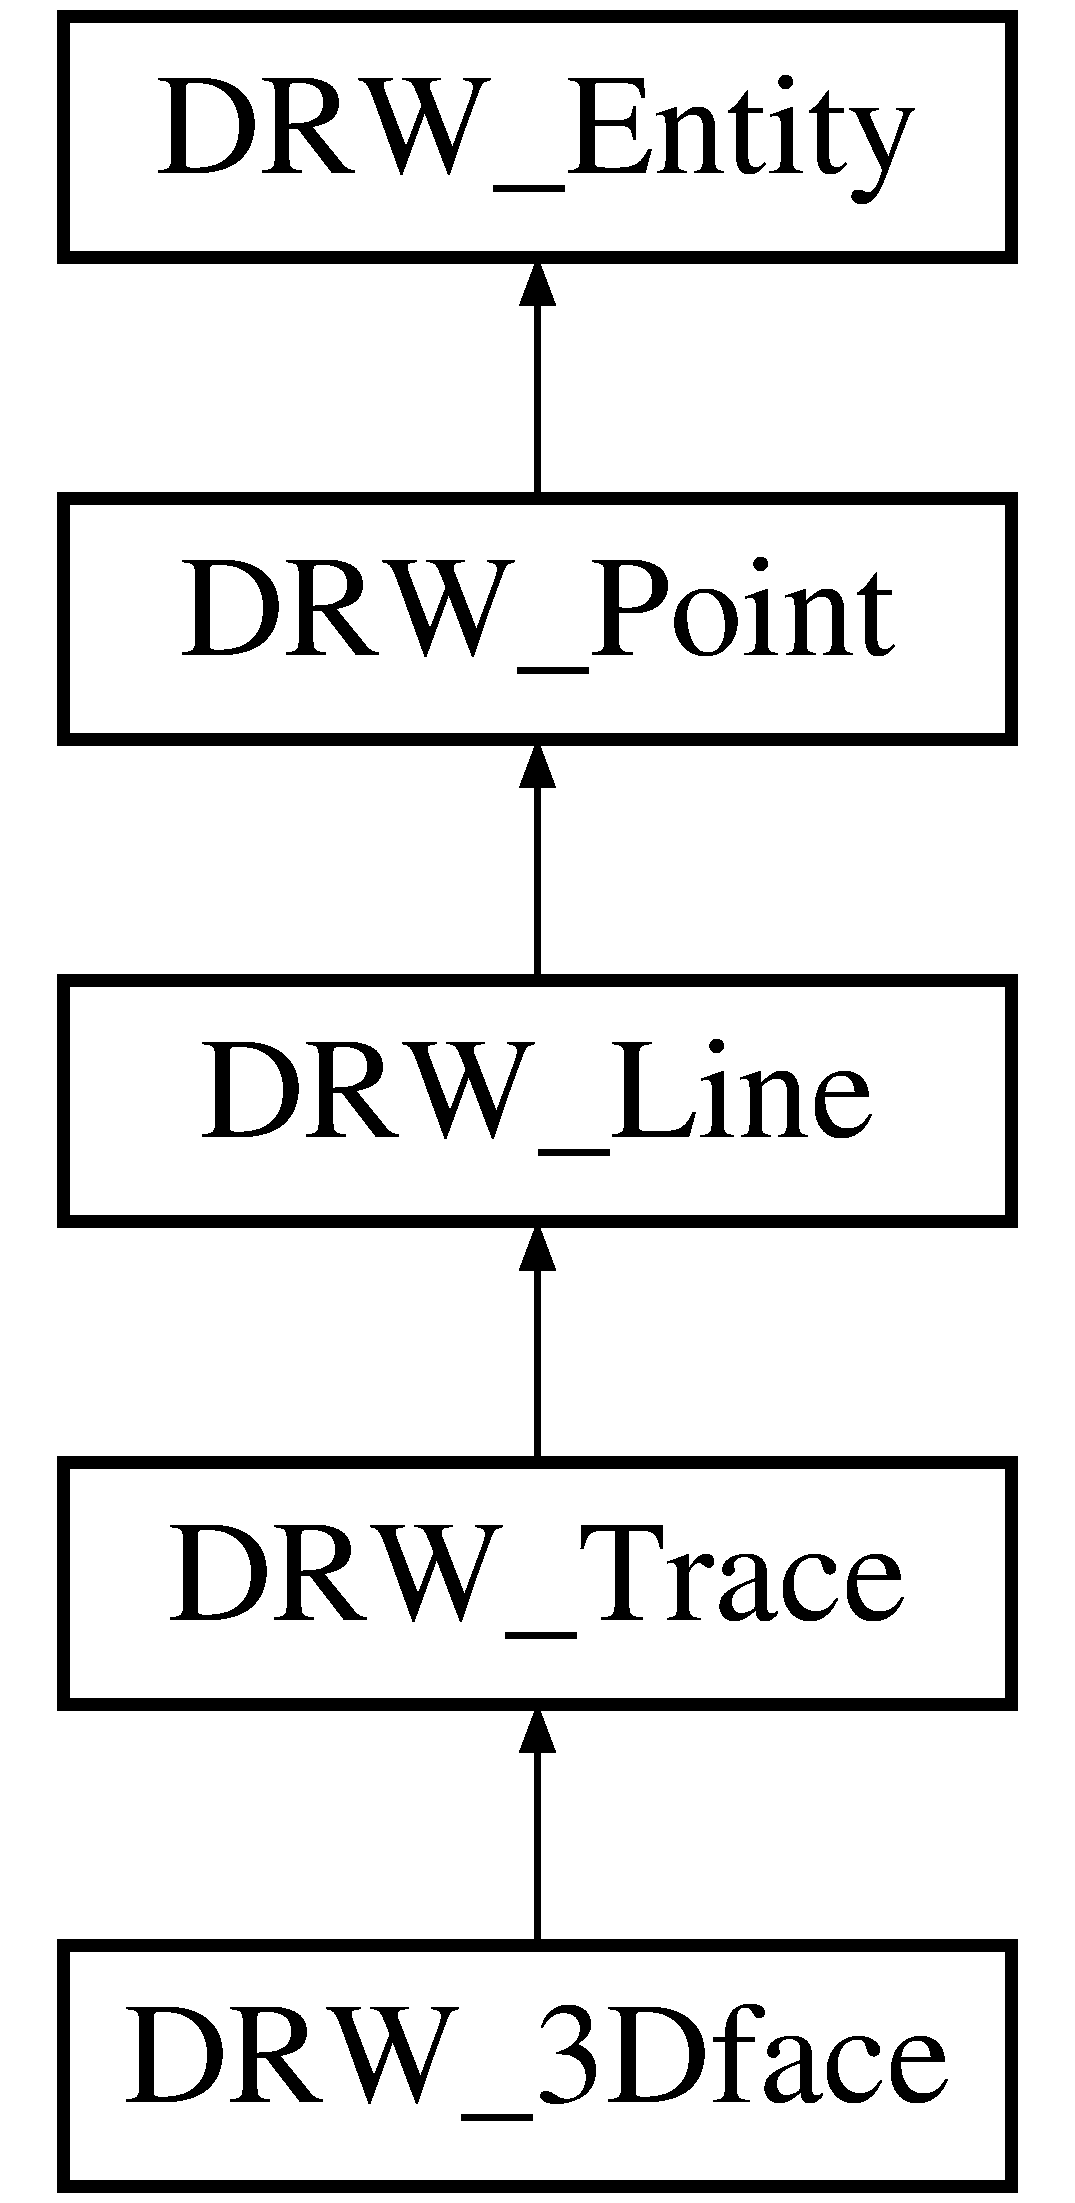
\includegraphics[height=5.000000cm]{da/dec/class_d_r_w__3_dface}
\end{center}
\end{figure}
\subsection*{Public Member Functions}
\begin{DoxyCompactItemize}
\item 
\hypertarget{class_d_r_w__3_dface_a56da97e5084ecff4a44fb96d268d32e6}{}const \hyperlink{class_d_r_w___coord}{D\+R\+W\+\_\+\+Coord} \& \hyperlink{class_d_r_w__3_dface_a56da97e5084ecff4a44fb96d268d32e6}{first\+Corner} ()\label{class_d_r_w__3_dface_a56da97e5084ecff4a44fb96d268d32e6}

\begin{DoxyCompactList}\small\item\em first corner in W\+C\+S \end{DoxyCompactList}\item 
\hypertarget{class_d_r_w__3_dface_a721316b57f076fb50ccd3117262519d6}{}const \hyperlink{class_d_r_w___coord}{D\+R\+W\+\_\+\+Coord} \& \hyperlink{class_d_r_w__3_dface_a721316b57f076fb50ccd3117262519d6}{second\+Corner} ()\label{class_d_r_w__3_dface_a721316b57f076fb50ccd3117262519d6}

\begin{DoxyCompactList}\small\item\em second corner in W\+C\+S \end{DoxyCompactList}\item 
\hypertarget{class_d_r_w__3_dface_ac88a266080ba7edfd54cb3c05097df2d}{}const \hyperlink{class_d_r_w___coord}{D\+R\+W\+\_\+\+Coord} \& \hyperlink{class_d_r_w__3_dface_ac88a266080ba7edfd54cb3c05097df2d}{third\+Corner} ()\label{class_d_r_w__3_dface_ac88a266080ba7edfd54cb3c05097df2d}

\begin{DoxyCompactList}\small\item\em third corner in W\+C\+S \end{DoxyCompactList}\item 
\hypertarget{class_d_r_w__3_dface_aba1e46ff30324167bfac371ace58a2f9}{}const \hyperlink{class_d_r_w___coord}{D\+R\+W\+\_\+\+Coord} \& \hyperlink{class_d_r_w__3_dface_aba1e46ff30324167bfac371ace58a2f9}{fourth\+Corner} ()\label{class_d_r_w__3_dface_aba1e46ff30324167bfac371ace58a2f9}

\begin{DoxyCompactList}\small\item\em fourth corner in W\+C\+S \end{DoxyCompactList}\item 
\hypertarget{class_d_r_w__3_dface_a7f7325421bb47d3e335e9e41237cf71d}{}Edge\+Flags \hyperlink{class_d_r_w__3_dface_a7f7325421bb47d3e335e9e41237cf71d}{edge\+Flags} ()\label{class_d_r_w__3_dface_a7f7325421bb47d3e335e9e41237cf71d}

\begin{DoxyCompactList}\small\item\em edge visibility flags \end{DoxyCompactList}\end{DoxyCompactItemize}
\subsection*{Public Attributes}
\begin{DoxyCompactItemize}
\item 
int \hyperlink{class_d_r_w__3_dface_a0fbb465670025bbd116aef1804fa5b44}{invisibleflag}
\end{DoxyCompactItemize}
\subsection*{Protected Member Functions}
\begin{DoxyCompactItemize}
\item 
\hypertarget{class_d_r_w__3_dface_a841b20016d7bf6d3221aa690fb477076}{}void \hyperlink{class_d_r_w__3_dface_a841b20016d7bf6d3221aa690fb477076}{parse\+Code} (int code, dxf\+Reader $\ast$reader)\label{class_d_r_w__3_dface_a841b20016d7bf6d3221aa690fb477076}

\begin{DoxyCompactList}\small\item\em interpret code in dxf reading process or dispatch to inherited class \end{DoxyCompactList}\item 
\hypertarget{class_d_r_w__3_dface_a728d8ad4840139bb826a67f1012b22ed}{}virtual bool \hyperlink{class_d_r_w__3_dface_a728d8ad4840139bb826a67f1012b22ed}{parse\+Dwg} (D\+R\+W\+::\+Version v, dwg\+Buffer $\ast$buf)\label{class_d_r_w__3_dface_a728d8ad4840139bb826a67f1012b22ed}

\begin{DoxyCompactList}\small\item\em interpret dwg data (was already determined to be part of this object) \end{DoxyCompactList}\end{DoxyCompactItemize}


\subsection{Detailed Description}
Class to handle 3dface entity. 

Class to handle 3dface entity \begin{DoxyAuthor}{Author}
Rallaz 
\end{DoxyAuthor}


\subsection{Member Data Documentation}
\hypertarget{class_d_r_w__3_dface_a0fbb465670025bbd116aef1804fa5b44}{}\index{D\+R\+W\+\_\+3\+Dface@{D\+R\+W\+\_\+3\+Dface}!invisibleflag@{invisibleflag}}
\index{invisibleflag@{invisibleflag}!D\+R\+W\+\_\+3\+Dface@{D\+R\+W\+\_\+3\+Dface}}
\subsubsection[{invisibleflag}]{\setlength{\rightskip}{0pt plus 5cm}int D\+R\+W\+\_\+3\+Dface\+::invisibleflag}\label{class_d_r_w__3_dface_a0fbb465670025bbd116aef1804fa5b44}
invisible edge flag, code 70 

The documentation for this class was generated from the following files\+:\begin{DoxyCompactItemize}
\item 
src/drw\+\_\+entities.\+h\item 
src/drw\+\_\+entities.\+cpp\end{DoxyCompactItemize}

\hypertarget{class_d_r_w___arc}{}\section{D\+R\+W\+\_\+\+Arc Class Reference}
\label{class_d_r_w___arc}\index{D\+R\+W\+\_\+\+Arc@{D\+R\+W\+\_\+\+Arc}}


Class to handle arc entity.  




{\ttfamily \#include $<$drw\+\_\+entities.\+h$>$}

Inheritance diagram for D\+R\+W\+\_\+\+Arc\+:\begin{figure}[H]
\begin{center}
\leavevmode
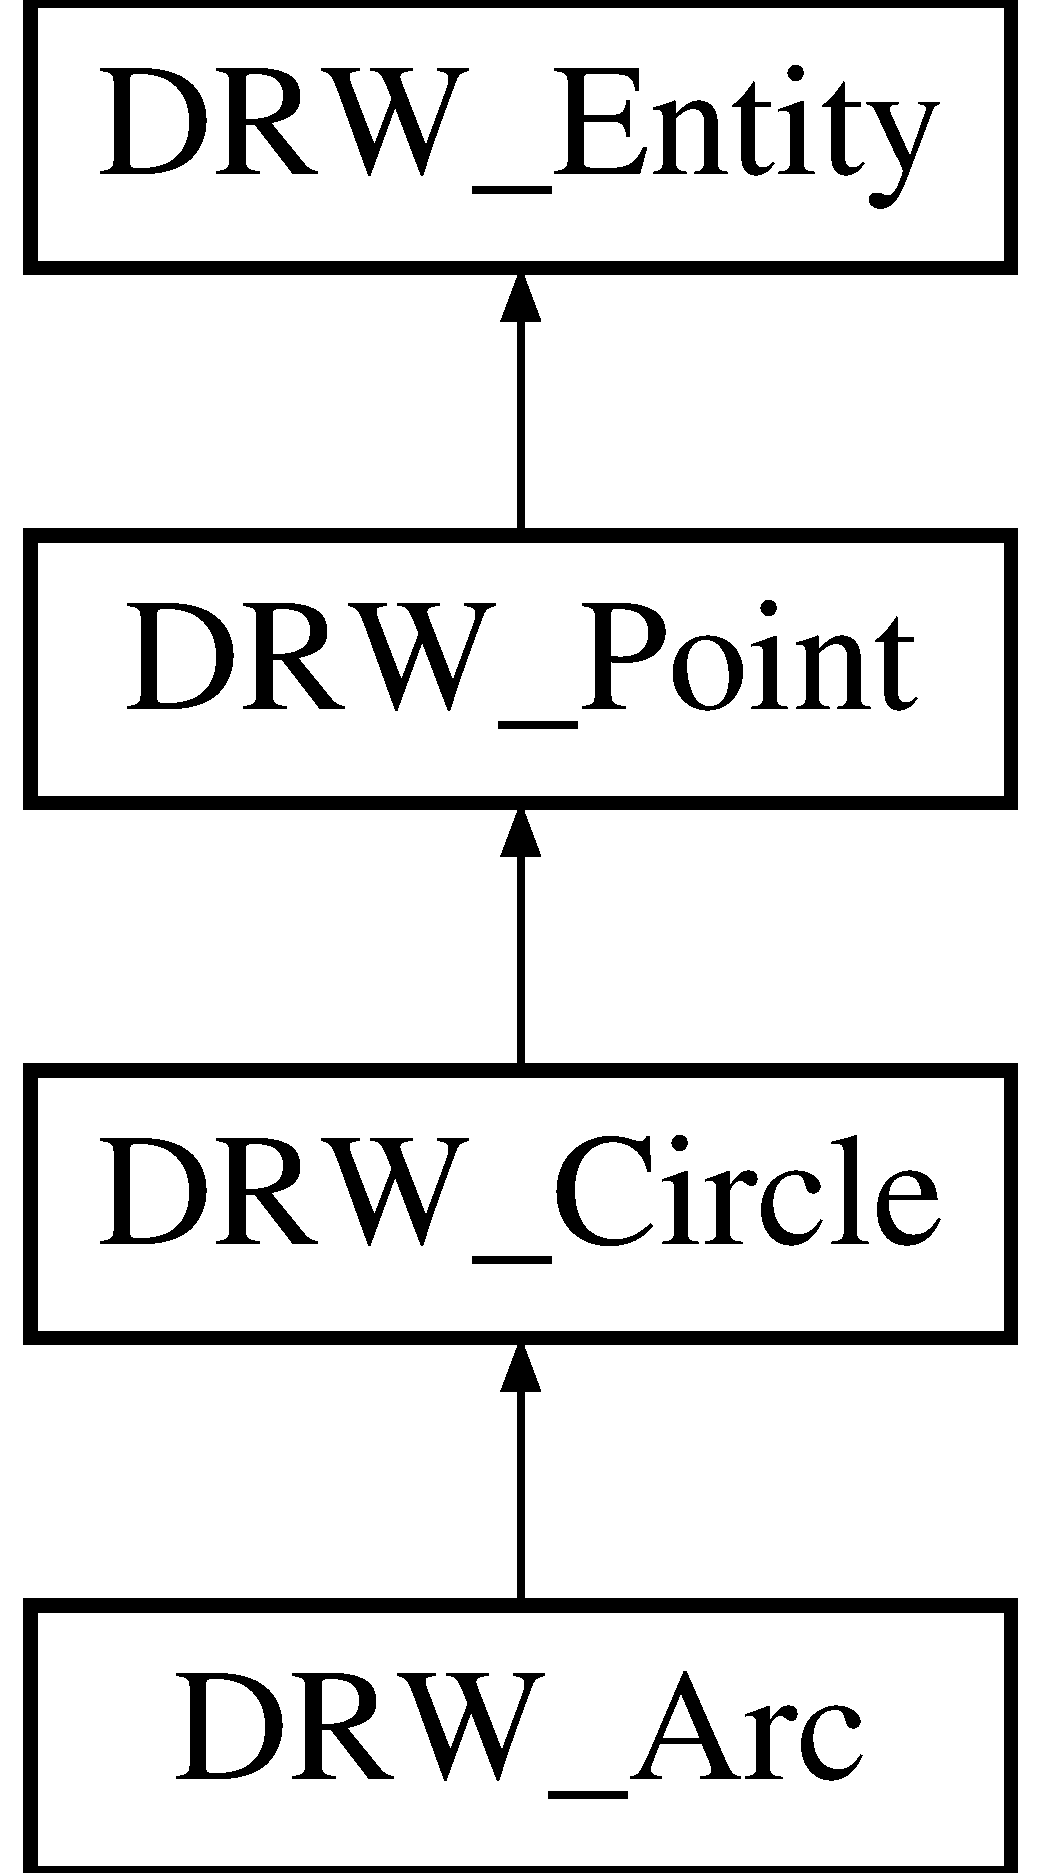
\includegraphics[height=4.000000cm]{d1/ddc/class_d_r_w___arc}
\end{center}
\end{figure}
\subsection*{Public Member Functions}
\begin{DoxyCompactItemize}
\item 
\hypertarget{class_d_r_w___arc_a1d2d880ea3dcfd52429d9a9c4cb680d2}{}const \hyperlink{class_d_r_w___coord}{D\+R\+W\+\_\+\+Coord} \& \hyperlink{class_d_r_w___arc_a1d2d880ea3dcfd52429d9a9c4cb680d2}{center} ()\label{class_d_r_w___arc_a1d2d880ea3dcfd52429d9a9c4cb680d2}

\begin{DoxyCompactList}\small\item\em center point in O\+C\+S \end{DoxyCompactList}\item 
\hypertarget{class_d_r_w___arc_a22792839d56bb40f5f01fcf8000f1c8d}{}double \hyperlink{class_d_r_w___arc_a22792839d56bb40f5f01fcf8000f1c8d}{radius} ()\label{class_d_r_w___arc_a22792839d56bb40f5f01fcf8000f1c8d}

\begin{DoxyCompactList}\small\item\em the radius of the circle \end{DoxyCompactList}\item 
\hypertarget{class_d_r_w___arc_adae2ce7765f7572c747ee13c82ef55a7}{}double \hyperlink{class_d_r_w___arc_adae2ce7765f7572c747ee13c82ef55a7}{start\+Angle} ()\label{class_d_r_w___arc_adae2ce7765f7572c747ee13c82ef55a7}

\begin{DoxyCompactList}\small\item\em start angle in radians \end{DoxyCompactList}\item 
\hypertarget{class_d_r_w___arc_aa11139680c3bc9d63eb266968d4aa5fb}{}double \hyperlink{class_d_r_w___arc_aa11139680c3bc9d63eb266968d4aa5fb}{end\+Angle} ()\label{class_d_r_w___arc_aa11139680c3bc9d63eb266968d4aa5fb}

\begin{DoxyCompactList}\small\item\em end angle in radians \end{DoxyCompactList}\item 
\hypertarget{class_d_r_w___arc_a59fbfc76b5fd2846a447a2f34c8ed1c0}{}double \hyperlink{class_d_r_w___arc_a59fbfc76b5fd2846a447a2f34c8ed1c0}{thick} ()\label{class_d_r_w___arc_a59fbfc76b5fd2846a447a2f34c8ed1c0}

\begin{DoxyCompactList}\small\item\em thickness \end{DoxyCompactList}\item 
\hypertarget{class_d_r_w___arc_adeaf1204c08b172ba08106b61f13d4eb}{}const \hyperlink{class_d_r_w___coord}{D\+R\+W\+\_\+\+Coord} \& \hyperlink{class_d_r_w___arc_adeaf1204c08b172ba08106b61f13d4eb}{extrusion} ()\label{class_d_r_w___arc_adeaf1204c08b172ba08106b61f13d4eb}

\begin{DoxyCompactList}\small\item\em extrusion \end{DoxyCompactList}\end{DoxyCompactItemize}
\subsection*{Public Attributes}
\begin{DoxyCompactItemize}
\item 
double \hyperlink{class_d_r_w___arc_a7718d55eb1ddd3c4038be5798f37570e}{staangle}
\item 
double \hyperlink{class_d_r_w___arc_a3425163b91e875fc7ffad0176e0e8183}{endangle}
\item 
int \hyperlink{class_d_r_w___arc_aaacaac1262bc3e4a2e83c13804d1cb00}{isccw}
\end{DoxyCompactItemize}
\subsection*{Protected Member Functions}
\begin{DoxyCompactItemize}
\item 
\hypertarget{class_d_r_w___arc_a837c22a41f1b3eff3c64b10faff85de5}{}void \hyperlink{class_d_r_w___arc_a837c22a41f1b3eff3c64b10faff85de5}{parse\+Code} (int code, dxf\+Reader $\ast$reader)\label{class_d_r_w___arc_a837c22a41f1b3eff3c64b10faff85de5}

\begin{DoxyCompactList}\small\item\em interpret code in dxf reading process or dispatch to inherited class \end{DoxyCompactList}\item 
\hypertarget{class_d_r_w___arc_ab76e7a51ddf6d330373a330d0d610069}{}virtual bool \hyperlink{class_d_r_w___arc_ab76e7a51ddf6d330373a330d0d610069}{parse\+Dwg} (D\+R\+W\+::\+Version v, dwg\+Buffer $\ast$buf)\label{class_d_r_w___arc_ab76e7a51ddf6d330373a330d0d610069}

\begin{DoxyCompactList}\small\item\em interpret dwg data (was already determined to be part of this object) \end{DoxyCompactList}\end{DoxyCompactItemize}


\subsection{Detailed Description}
Class to handle arc entity. 

Class to handle arc entity \begin{DoxyAuthor}{Author}
Rallaz 
\end{DoxyAuthor}


\subsection{Member Data Documentation}
\hypertarget{class_d_r_w___arc_a3425163b91e875fc7ffad0176e0e8183}{}\index{D\+R\+W\+\_\+\+Arc@{D\+R\+W\+\_\+\+Arc}!endangle@{endangle}}
\index{endangle@{endangle}!D\+R\+W\+\_\+\+Arc@{D\+R\+W\+\_\+\+Arc}}
\subsubsection[{endangle}]{\setlength{\rightskip}{0pt plus 5cm}double D\+R\+W\+\_\+\+Arc\+::endangle}\label{class_d_r_w___arc_a3425163b91e875fc7ffad0176e0e8183}
end angle, code 51 in radians \hypertarget{class_d_r_w___arc_aaacaac1262bc3e4a2e83c13804d1cb00}{}\index{D\+R\+W\+\_\+\+Arc@{D\+R\+W\+\_\+\+Arc}!isccw@{isccw}}
\index{isccw@{isccw}!D\+R\+W\+\_\+\+Arc@{D\+R\+W\+\_\+\+Arc}}
\subsubsection[{isccw}]{\setlength{\rightskip}{0pt plus 5cm}int D\+R\+W\+\_\+\+Arc\+::isccw}\label{class_d_r_w___arc_aaacaac1262bc3e4a2e83c13804d1cb00}
is counter clockwise arc?, only used in hatch, code 73 \hypertarget{class_d_r_w___arc_a7718d55eb1ddd3c4038be5798f37570e}{}\index{D\+R\+W\+\_\+\+Arc@{D\+R\+W\+\_\+\+Arc}!staangle@{staangle}}
\index{staangle@{staangle}!D\+R\+W\+\_\+\+Arc@{D\+R\+W\+\_\+\+Arc}}
\subsubsection[{staangle}]{\setlength{\rightskip}{0pt plus 5cm}double D\+R\+W\+\_\+\+Arc\+::staangle}\label{class_d_r_w___arc_a7718d55eb1ddd3c4038be5798f37570e}
start angle, code 50 in radians 

The documentation for this class was generated from the following files\+:\begin{DoxyCompactItemize}
\item 
src/drw\+\_\+entities.\+h\item 
src/drw\+\_\+entities.\+cpp\end{DoxyCompactItemize}

\hypertarget{class_d_r_w___block}{}\section{D\+R\+W\+\_\+\+Block Class Reference}
\label{class_d_r_w___block}\index{D\+R\+W\+\_\+\+Block@{D\+R\+W\+\_\+\+Block}}


Class to handle block entries.  




{\ttfamily \#include $<$drw\+\_\+entities.\+h$>$}

Inheritance diagram for D\+R\+W\+\_\+\+Block\+:\begin{figure}[H]
\begin{center}
\leavevmode
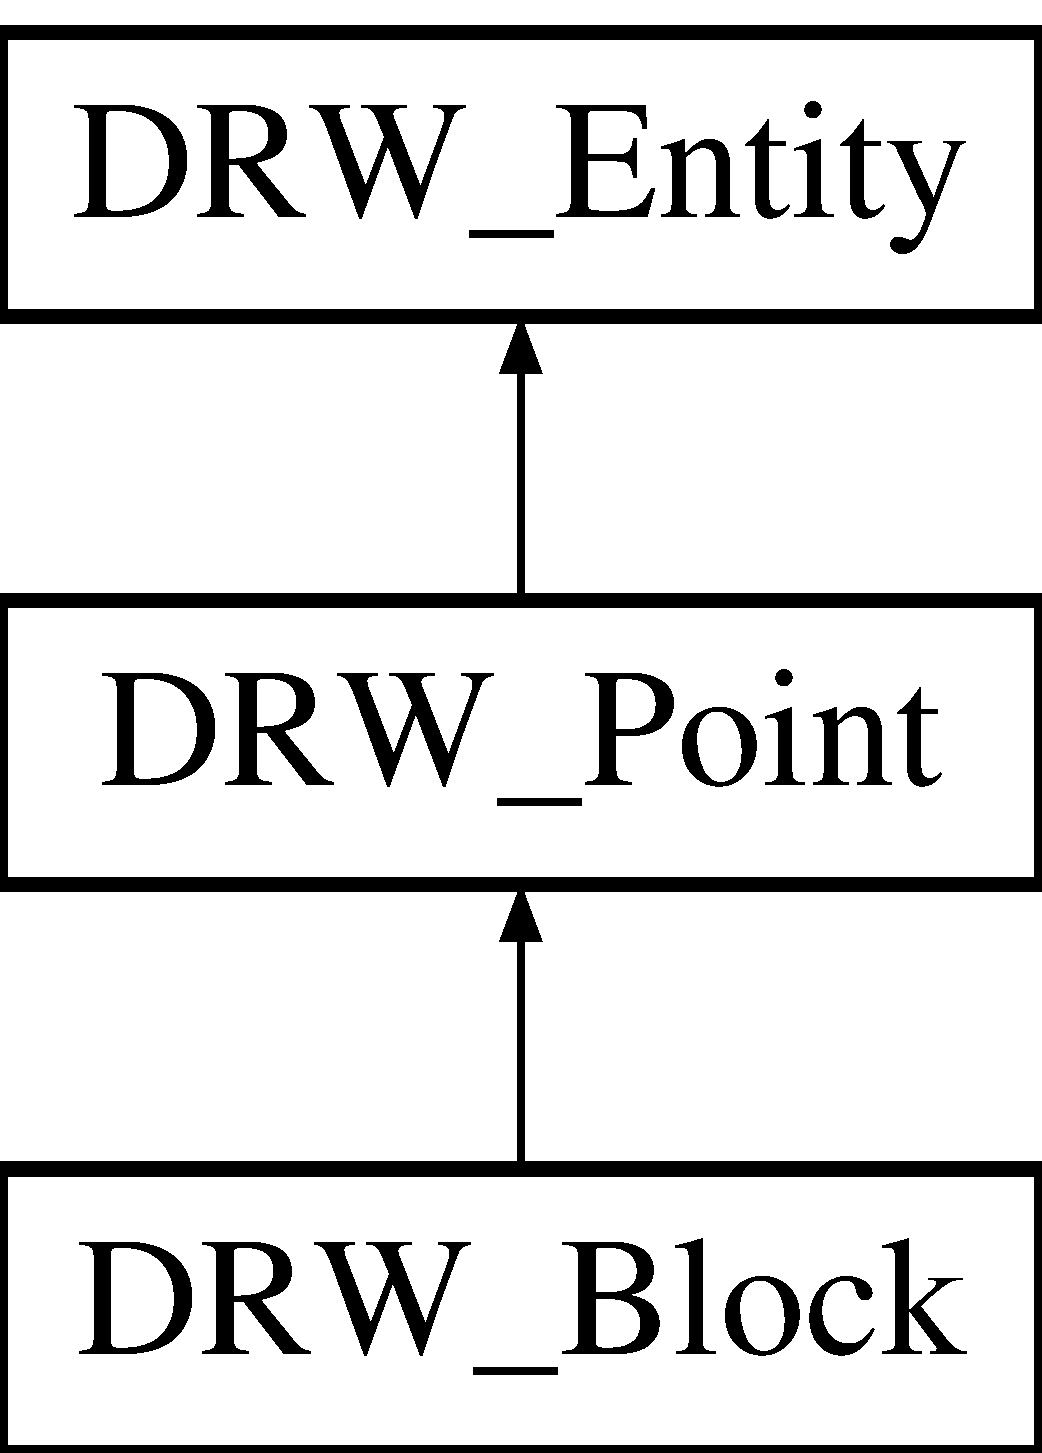
\includegraphics[height=3.000000cm]{da/d3b/class_d_r_w___block}
\end{center}
\end{figure}
\subsection*{Public Attributes}
\begin{DoxyCompactItemize}
\item 
U\+T\+F8\+S\+T\+R\+I\+N\+G \hyperlink{class_d_r_w___block_a574a37d634655f8ea5526a80e842a66a}{name}
\item 
int \hyperlink{class_d_r_w___block_a17bb4c01376f4b30b8d3ce36863b3ae3}{flags}
\end{DoxyCompactItemize}
\subsection*{Additional Inherited Members}


\subsection{Detailed Description}
Class to handle block entries. 

Class to handle block entries \begin{DoxyAuthor}{Author}
Rallaz 
\end{DoxyAuthor}


\subsection{Member Data Documentation}
\hypertarget{class_d_r_w___block_a17bb4c01376f4b30b8d3ce36863b3ae3}{}\index{D\+R\+W\+\_\+\+Block@{D\+R\+W\+\_\+\+Block}!flags@{flags}}
\index{flags@{flags}!D\+R\+W\+\_\+\+Block@{D\+R\+W\+\_\+\+Block}}
\subsubsection[{flags}]{\setlength{\rightskip}{0pt plus 5cm}int D\+R\+W\+\_\+\+Block\+::flags}\label{class_d_r_w___block_a17bb4c01376f4b30b8d3ce36863b3ae3}
block type, code 70 \hypertarget{class_d_r_w___block_a574a37d634655f8ea5526a80e842a66a}{}\index{D\+R\+W\+\_\+\+Block@{D\+R\+W\+\_\+\+Block}!name@{name}}
\index{name@{name}!D\+R\+W\+\_\+\+Block@{D\+R\+W\+\_\+\+Block}}
\subsubsection[{name}]{\setlength{\rightskip}{0pt plus 5cm}U\+T\+F8\+S\+T\+R\+I\+N\+G D\+R\+W\+\_\+\+Block\+::name}\label{class_d_r_w___block_a574a37d634655f8ea5526a80e842a66a}
block name, code 2 

The documentation for this class was generated from the following files\+:\begin{DoxyCompactItemize}
\item 
src/drw\+\_\+entities.\+h\item 
src/drw\+\_\+entities.\+cpp\end{DoxyCompactItemize}

\hypertarget{class_d_r_w___block___record}{}\section{D\+R\+W\+\_\+\+Block\+\_\+\+Record Class Reference}
\label{class_d_r_w___block___record}\index{D\+R\+W\+\_\+\+Block\+\_\+\+Record@{D\+R\+W\+\_\+\+Block\+\_\+\+Record}}


Class to handle layer entries.  




{\ttfamily \#include $<$drw\+\_\+objects.\+h$>$}

Inheritance diagram for D\+R\+W\+\_\+\+Block\+\_\+\+Record\+:\begin{figure}[H]
\begin{center}
\leavevmode
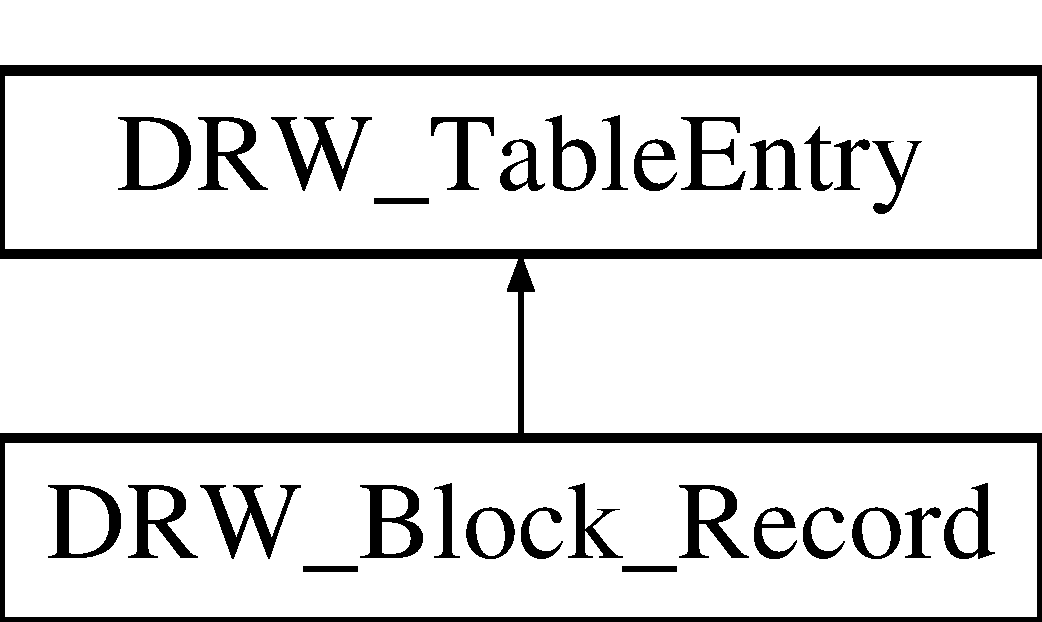
\includegraphics[height=2.000000cm]{d9/db1/class_d_r_w___block___record}
\end{center}
\end{figure}
\subsection*{Public Attributes}
\begin{DoxyCompactItemize}
\item 
int \hyperlink{class_d_r_w___block___record_ad4a51c93d03294546b648f0b866577d7}{ins\+Units}
\item 
\hyperlink{class_d_r_w___coord}{D\+R\+W\+\_\+\+Coord} \hyperlink{class_d_r_w___block___record_a95b52334c0b306ac7c07f2d66f13d1cf}{base\+Point}
\end{DoxyCompactItemize}
\subsection*{Additional Inherited Members}


\subsection{Detailed Description}
Class to handle layer entries. 

Class to handle block record table entries \begin{DoxyAuthor}{Author}
Rallaz 
\end{DoxyAuthor}


\subsection{Member Data Documentation}
\hypertarget{class_d_r_w___block___record_a95b52334c0b306ac7c07f2d66f13d1cf}{}\index{D\+R\+W\+\_\+\+Block\+\_\+\+Record@{D\+R\+W\+\_\+\+Block\+\_\+\+Record}!base\+Point@{base\+Point}}
\index{base\+Point@{base\+Point}!D\+R\+W\+\_\+\+Block\+\_\+\+Record@{D\+R\+W\+\_\+\+Block\+\_\+\+Record}}
\subsubsection[{base\+Point}]{\setlength{\rightskip}{0pt plus 5cm}{\bf D\+R\+W\+\_\+\+Coord} D\+R\+W\+\_\+\+Block\+\_\+\+Record\+::base\+Point}\label{class_d_r_w___block___record_a95b52334c0b306ac7c07f2d66f13d1cf}
block insertion base point dwg only \hypertarget{class_d_r_w___block___record_ad4a51c93d03294546b648f0b866577d7}{}\index{D\+R\+W\+\_\+\+Block\+\_\+\+Record@{D\+R\+W\+\_\+\+Block\+\_\+\+Record}!ins\+Units@{ins\+Units}}
\index{ins\+Units@{ins\+Units}!D\+R\+W\+\_\+\+Block\+\_\+\+Record@{D\+R\+W\+\_\+\+Block\+\_\+\+Record}}
\subsubsection[{ins\+Units}]{\setlength{\rightskip}{0pt plus 5cm}int D\+R\+W\+\_\+\+Block\+\_\+\+Record\+::ins\+Units}\label{class_d_r_w___block___record_ad4a51c93d03294546b648f0b866577d7}
block insertion units, code 70 of block\+\_\+record 

The documentation for this class was generated from the following files\+:\begin{DoxyCompactItemize}
\item 
src/drw\+\_\+objects.\+h\item 
src/drw\+\_\+objects.\+cpp\end{DoxyCompactItemize}

\hypertarget{class_d_r_w___circle}{}\section{D\+R\+W\+\_\+\+Circle Class Reference}
\label{class_d_r_w___circle}\index{D\+R\+W\+\_\+\+Circle@{D\+R\+W\+\_\+\+Circle}}


Class to handle circle entity.  




{\ttfamily \#include $<$drw\+\_\+entities.\+h$>$}

Inheritance diagram for D\+R\+W\+\_\+\+Circle\+:\begin{figure}[H]
\begin{center}
\leavevmode
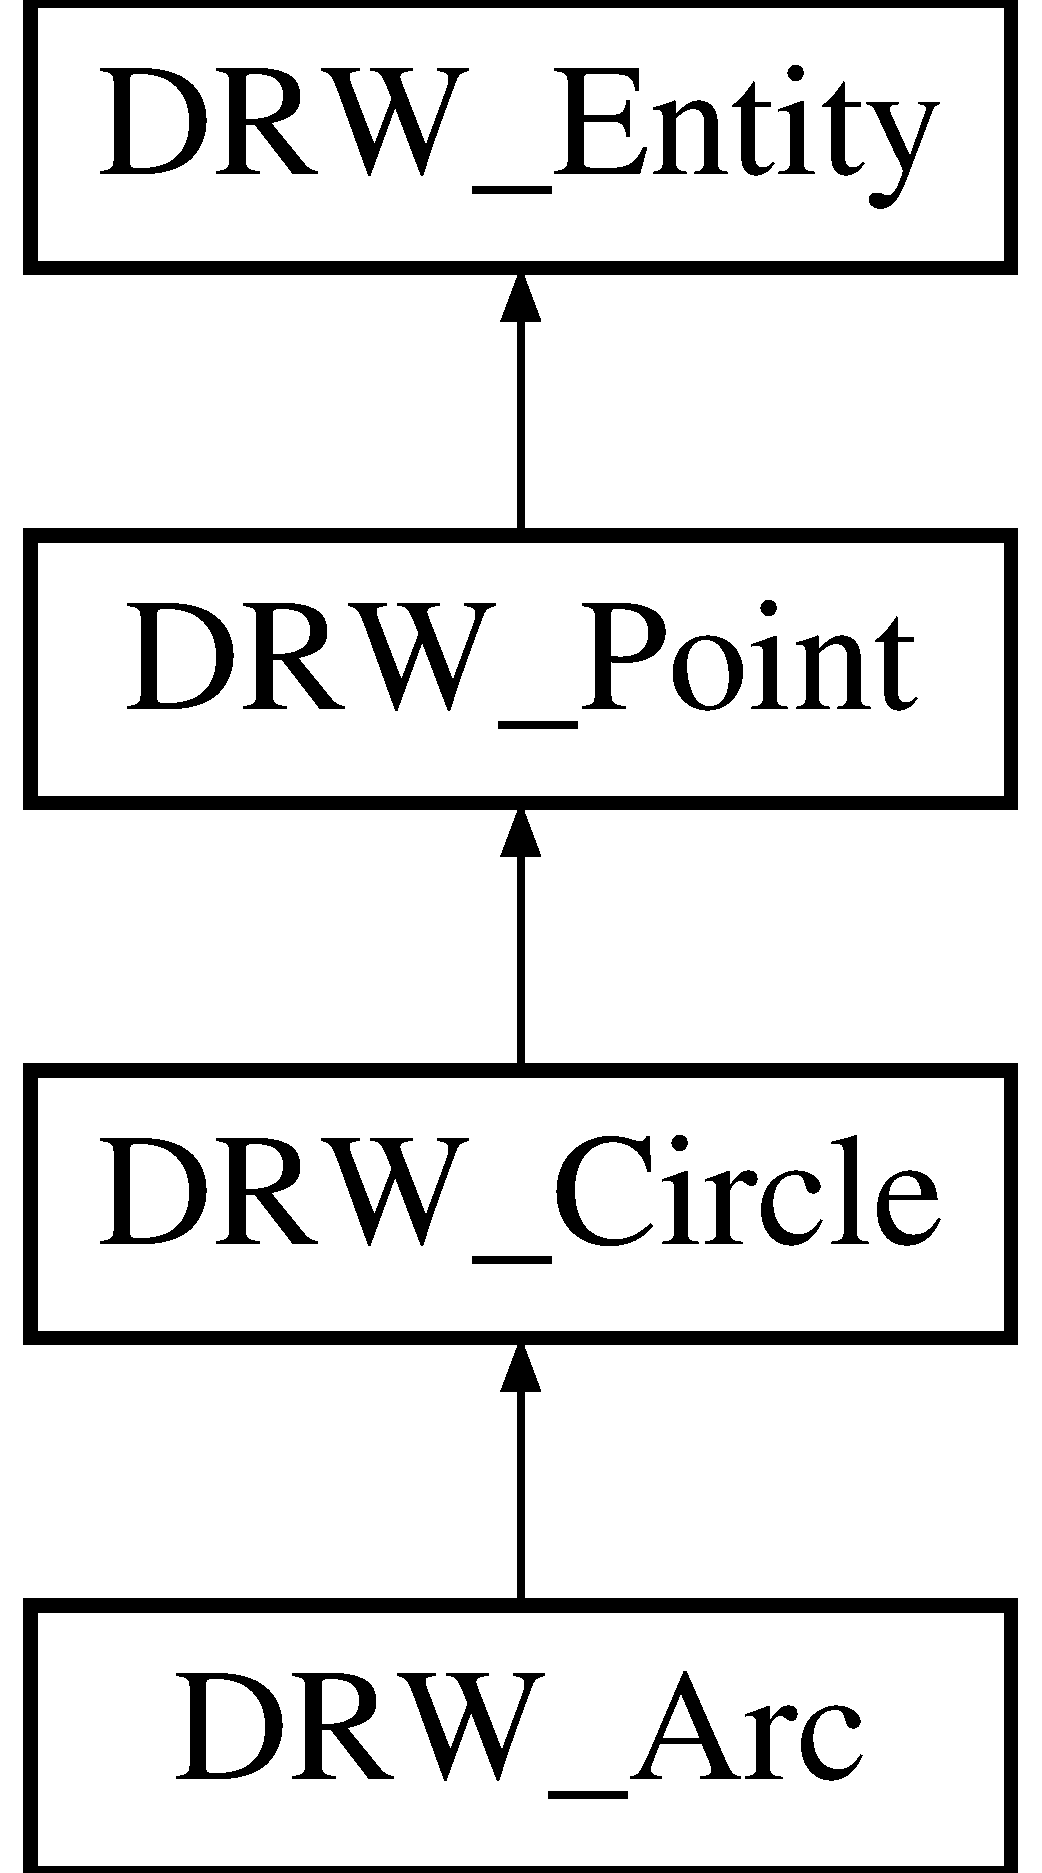
\includegraphics[height=4.000000cm]{de/dff/class_d_r_w___circle}
\end{center}
\end{figure}
\subsection*{Public Attributes}
\begin{DoxyCompactItemize}
\item 
double \hyperlink{class_d_r_w___circle_ab431594544fbe949dd44cbb79e1a7237}{radious}
\end{DoxyCompactItemize}
\subsection*{Additional Inherited Members}


\subsection{Detailed Description}
Class to handle circle entity. 

Class to handle circle entity \begin{DoxyAuthor}{Author}
Rallaz 
\end{DoxyAuthor}


\subsection{Member Data Documentation}
\hypertarget{class_d_r_w___circle_ab431594544fbe949dd44cbb79e1a7237}{}\index{D\+R\+W\+\_\+\+Circle@{D\+R\+W\+\_\+\+Circle}!radious@{radious}}
\index{radious@{radious}!D\+R\+W\+\_\+\+Circle@{D\+R\+W\+\_\+\+Circle}}
\subsubsection[{radious}]{\setlength{\rightskip}{0pt plus 5cm}double D\+R\+W\+\_\+\+Circle\+::radious}\label{class_d_r_w___circle_ab431594544fbe949dd44cbb79e1a7237}
radius, code 40 

The documentation for this class was generated from the following files\+:\begin{DoxyCompactItemize}
\item 
src/drw\+\_\+entities.\+h\item 
src/drw\+\_\+entities.\+cpp\end{DoxyCompactItemize}

\hypertarget{class_d_r_w___class}{}\section{D\+R\+W\+\_\+\+Class Class Reference}
\label{class_d_r_w___class}\index{D\+R\+W\+\_\+\+Class@{D\+R\+W\+\_\+\+Class}}


Class to handle classes entries.  




{\ttfamily \#include $<$drw\+\_\+classes.\+h$>$}

\subsection*{Public Attributes}
\begin{DoxyCompactItemize}
\item 
U\+T\+F8\+S\+T\+R\+I\+N\+G \hyperlink{class_d_r_w___class_ac3470fefc02faf7f2eb5dff1dac7af9a}{rec\+Nane}
\item 
U\+T\+F8\+S\+T\+R\+I\+N\+G \hyperlink{class_d_r_w___class_acde079b8bf4ff8e12ddbb592d492a22f}{class\+Name}
\item 
U\+T\+F8\+S\+T\+R\+I\+N\+G \hyperlink{class_d_r_w___class_a15b27bae29a5245c739f3de255e65760}{app\+Name}
\item 
int \hyperlink{class_d_r_w___class_a6a472aad89b499e5b0dd4a5c2c07b735}{proxy\+Capabilities}
\item 
int \hyperlink{class_d_r_w___class_a093a40e69719110340d4954cdcfde582}{proxy\+Flag}
\item 
int \hyperlink{class_d_r_w___class_ab6d13ec9b7720e2b04533d0adbb6b1f6}{entity\+Flag}
\end{DoxyCompactItemize}


\subsection{Detailed Description}
Class to handle classes entries. 

Class to handle classes table entries T\+O\+D\+O\+: verify the dxf read/write part \begin{DoxyAuthor}{Author}
Rallaz 
\end{DoxyAuthor}


\subsection{Member Data Documentation}
\hypertarget{class_d_r_w___class_a15b27bae29a5245c739f3de255e65760}{}\index{D\+R\+W\+\_\+\+Class@{D\+R\+W\+\_\+\+Class}!app\+Name@{app\+Name}}
\index{app\+Name@{app\+Name}!D\+R\+W\+\_\+\+Class@{D\+R\+W\+\_\+\+Class}}
\subsubsection[{app\+Name}]{\setlength{\rightskip}{0pt plus 5cm}U\+T\+F8\+S\+T\+R\+I\+N\+G D\+R\+W\+\_\+\+Class\+::app\+Name}\label{class_d_r_w___class_a15b27bae29a5245c739f3de255e65760}
app name, code 3 \hypertarget{class_d_r_w___class_acde079b8bf4ff8e12ddbb592d492a22f}{}\index{D\+R\+W\+\_\+\+Class@{D\+R\+W\+\_\+\+Class}!class\+Name@{class\+Name}}
\index{class\+Name@{class\+Name}!D\+R\+W\+\_\+\+Class@{D\+R\+W\+\_\+\+Class}}
\subsubsection[{class\+Name}]{\setlength{\rightskip}{0pt plus 5cm}U\+T\+F8\+S\+T\+R\+I\+N\+G D\+R\+W\+\_\+\+Class\+::class\+Name}\label{class_d_r_w___class_acde079b8bf4ff8e12ddbb592d492a22f}
C++ class name, code 2 \hypertarget{class_d_r_w___class_ab6d13ec9b7720e2b04533d0adbb6b1f6}{}\index{D\+R\+W\+\_\+\+Class@{D\+R\+W\+\_\+\+Class}!entity\+Flag@{entity\+Flag}}
\index{entity\+Flag@{entity\+Flag}!D\+R\+W\+\_\+\+Class@{D\+R\+W\+\_\+\+Class}}
\subsubsection[{entity\+Flag}]{\setlength{\rightskip}{0pt plus 5cm}int D\+R\+W\+\_\+\+Class\+::entity\+Flag}\label{class_d_r_w___class_ab6d13ec9b7720e2b04533d0adbb6b1f6}
entity flag, code 281 (0 object, 1 entity) \hypertarget{class_d_r_w___class_a6a472aad89b499e5b0dd4a5c2c07b735}{}\index{D\+R\+W\+\_\+\+Class@{D\+R\+W\+\_\+\+Class}!proxy\+Capabilities@{proxy\+Capabilities}}
\index{proxy\+Capabilities@{proxy\+Capabilities}!D\+R\+W\+\_\+\+Class@{D\+R\+W\+\_\+\+Class}}
\subsubsection[{proxy\+Capabilities}]{\setlength{\rightskip}{0pt plus 5cm}int D\+R\+W\+\_\+\+Class\+::proxy\+Capabilities}\label{class_d_r_w___class_a6a472aad89b499e5b0dd4a5c2c07b735}
proxy capabilities, code 90 \hypertarget{class_d_r_w___class_a093a40e69719110340d4954cdcfde582}{}\index{D\+R\+W\+\_\+\+Class@{D\+R\+W\+\_\+\+Class}!proxy\+Flag@{proxy\+Flag}}
\index{proxy\+Flag@{proxy\+Flag}!D\+R\+W\+\_\+\+Class@{D\+R\+W\+\_\+\+Class}}
\subsubsection[{proxy\+Flag}]{\setlength{\rightskip}{0pt plus 5cm}int D\+R\+W\+\_\+\+Class\+::proxy\+Flag}\label{class_d_r_w___class_a093a40e69719110340d4954cdcfde582}
proxy flag (app loaded on save), code 280 \hypertarget{class_d_r_w___class_ac3470fefc02faf7f2eb5dff1dac7af9a}{}\index{D\+R\+W\+\_\+\+Class@{D\+R\+W\+\_\+\+Class}!rec\+Nane@{rec\+Nane}}
\index{rec\+Nane@{rec\+Nane}!D\+R\+W\+\_\+\+Class@{D\+R\+W\+\_\+\+Class}}
\subsubsection[{rec\+Nane}]{\setlength{\rightskip}{0pt plus 5cm}U\+T\+F8\+S\+T\+R\+I\+N\+G D\+R\+W\+\_\+\+Class\+::rec\+Nane}\label{class_d_r_w___class_ac3470fefc02faf7f2eb5dff1dac7af9a}
record name, code 1 

The documentation for this class was generated from the following files\+:\begin{DoxyCompactItemize}
\item 
src/drw\+\_\+classes.\+h\item 
src/drw\+\_\+classes.\+cpp\end{DoxyCompactItemize}

\hypertarget{class_d_r_w___coord}{}\section{D\+R\+W\+\_\+\+Coord Class Reference}
\label{class_d_r_w___coord}\index{D\+R\+W\+\_\+\+Coord@{D\+R\+W\+\_\+\+Coord}}


Class to handle 3\+D coordinate point.  




{\ttfamily \#include $<$drw\+\_\+base.\+h$>$}

\subsection*{Public Member Functions}
\begin{DoxyCompactItemize}
\item 
\hyperlink{class_d_r_w___coord}{D\+R\+W\+\_\+\+Coord} \hyperlink{class_d_r_w___coord_a437b497bab4345ae2df8dc5d89bf865a}{operator=} (const \hyperlink{class_d_r_w___coord}{D\+R\+W\+\_\+\+Coord} \&data)
\end{DoxyCompactItemize}


\subsection{Detailed Description}
Class to handle 3\+D coordinate point. 

Class to handle 3\+D coordinate point \begin{DoxyAuthor}{Author}
Rallaz 
\end{DoxyAuthor}


\subsection{Member Function Documentation}
\hypertarget{class_d_r_w___coord_a437b497bab4345ae2df8dc5d89bf865a}{}\index{D\+R\+W\+\_\+\+Coord@{D\+R\+W\+\_\+\+Coord}!operator=@{operator=}}
\index{operator=@{operator=}!D\+R\+W\+\_\+\+Coord@{D\+R\+W\+\_\+\+Coord}}
\subsubsection[{operator=}]{\setlength{\rightskip}{0pt plus 5cm}{\bf D\+R\+W\+\_\+\+Coord} D\+R\+W\+\_\+\+Coord\+::operator= (
\begin{DoxyParamCaption}
\item[{const {\bf D\+R\+W\+\_\+\+Coord} \&}]{data}
\end{DoxyParamCaption}
)\hspace{0.3cm}{\ttfamily [inline]}}\label{class_d_r_w___coord_a437b497bab4345ae2df8dc5d89bf865a}
convert to unitary vector 

The documentation for this class was generated from the following file\+:\begin{DoxyCompactItemize}
\item 
src/drw\+\_\+base.\+h\end{DoxyCompactItemize}

\hypertarget{class_d_r_w___dim_aligned}{}\section{D\+R\+W\+\_\+\+Dim\+Aligned Class Reference}
\label{class_d_r_w___dim_aligned}\index{D\+R\+W\+\_\+\+Dim\+Aligned@{D\+R\+W\+\_\+\+Dim\+Aligned}}


Class to handle aligned dimension entity.  




{\ttfamily \#include $<$drw\+\_\+entities.\+h$>$}

Inheritance diagram for D\+R\+W\+\_\+\+Dim\+Aligned\+:\begin{figure}[H]
\begin{center}
\leavevmode
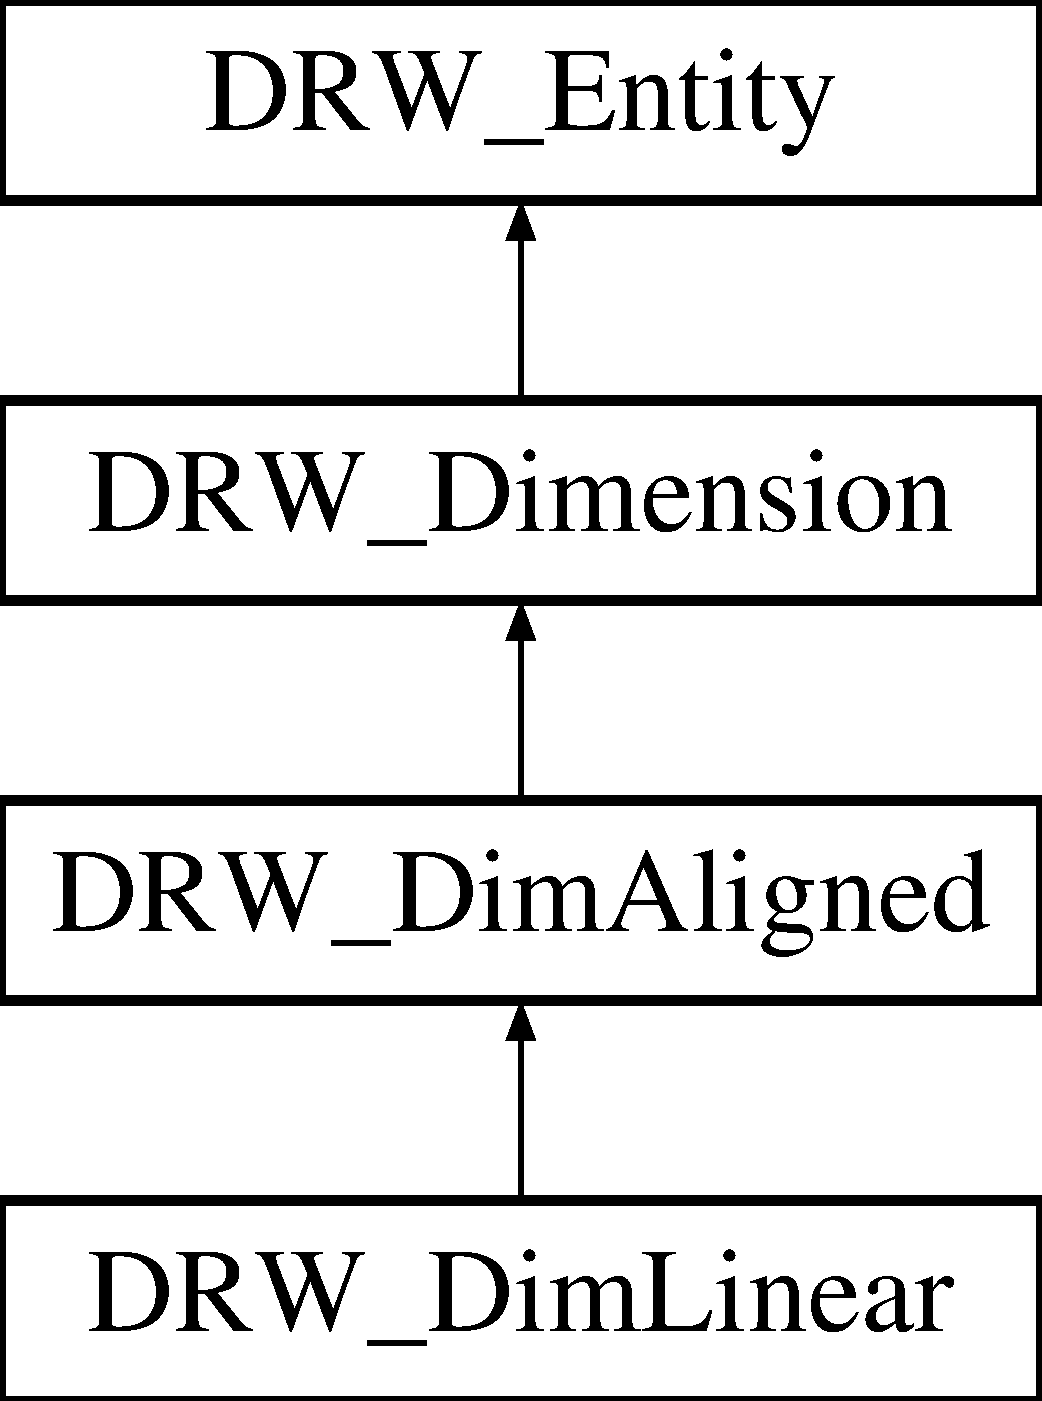
\includegraphics[height=4.000000cm]{d2/dcb/class_d_r_w___dim_aligned}
\end{center}
\end{figure}
\subsection*{Public Member Functions}
\begin{DoxyCompactItemize}
\item 
\hyperlink{class_d_r_w___coord}{D\+R\+W\+\_\+\+Coord} \hyperlink{class_d_r_w___dim_aligned_abbd897f18dec2dcded4a6c28ac08ae69}{get\+Clonepoint} () const 
\item 
\hyperlink{class_d_r_w___coord}{D\+R\+W\+\_\+\+Coord} \hyperlink{class_d_r_w___dim_aligned_ab59c46ec3dde19b8de90ca9065bc7e89}{get\+Dim\+Point} () const 
\item 
\hyperlink{class_d_r_w___coord}{D\+R\+W\+\_\+\+Coord} \hyperlink{class_d_r_w___dim_aligned_a3e3a2f5aa773efe06e349355b9ed0b43}{get\+Def1\+Point} () const 
\item 
\hyperlink{class_d_r_w___coord}{D\+R\+W\+\_\+\+Coord} \hyperlink{class_d_r_w___dim_aligned_aef8ab998257cf7ac609b8b3783af9e03}{get\+Def2\+Point} () const 
\end{DoxyCompactItemize}
\subsection*{Additional Inherited Members}


\subsection{Detailed Description}
Class to handle aligned dimension entity. 

Class to handle aligned dimension entity \begin{DoxyAuthor}{Author}
Rallaz 
\end{DoxyAuthor}


\subsection{Member Function Documentation}
\hypertarget{class_d_r_w___dim_aligned_abbd897f18dec2dcded4a6c28ac08ae69}{}\index{D\+R\+W\+\_\+\+Dim\+Aligned@{D\+R\+W\+\_\+\+Dim\+Aligned}!get\+Clonepoint@{get\+Clonepoint}}
\index{get\+Clonepoint@{get\+Clonepoint}!D\+R\+W\+\_\+\+Dim\+Aligned@{D\+R\+W\+\_\+\+Dim\+Aligned}}
\subsubsection[{get\+Clonepoint}]{\setlength{\rightskip}{0pt plus 5cm}{\bf D\+R\+W\+\_\+\+Coord} D\+R\+W\+\_\+\+Dim\+Aligned\+::get\+Clonepoint (
\begin{DoxyParamCaption}
{}
\end{DoxyParamCaption}
) const\hspace{0.3cm}{\ttfamily [inline]}}\label{class_d_r_w___dim_aligned_abbd897f18dec2dcded4a6c28ac08ae69}
Insertion for clones (Baseline \& Continue), 12, 22 \& 32 \hypertarget{class_d_r_w___dim_aligned_a3e3a2f5aa773efe06e349355b9ed0b43}{}\index{D\+R\+W\+\_\+\+Dim\+Aligned@{D\+R\+W\+\_\+\+Dim\+Aligned}!get\+Def1\+Point@{get\+Def1\+Point}}
\index{get\+Def1\+Point@{get\+Def1\+Point}!D\+R\+W\+\_\+\+Dim\+Aligned@{D\+R\+W\+\_\+\+Dim\+Aligned}}
\subsubsection[{get\+Def1\+Point}]{\setlength{\rightskip}{0pt plus 5cm}{\bf D\+R\+W\+\_\+\+Coord} D\+R\+W\+\_\+\+Dim\+Aligned\+::get\+Def1\+Point (
\begin{DoxyParamCaption}
{}
\end{DoxyParamCaption}
) const\hspace{0.3cm}{\ttfamily [inline]}}\label{class_d_r_w___dim_aligned_a3e3a2f5aa773efe06e349355b9ed0b43}
Definition point 1, code 13, 23 \& 33 \hypertarget{class_d_r_w___dim_aligned_aef8ab998257cf7ac609b8b3783af9e03}{}\index{D\+R\+W\+\_\+\+Dim\+Aligned@{D\+R\+W\+\_\+\+Dim\+Aligned}!get\+Def2\+Point@{get\+Def2\+Point}}
\index{get\+Def2\+Point@{get\+Def2\+Point}!D\+R\+W\+\_\+\+Dim\+Aligned@{D\+R\+W\+\_\+\+Dim\+Aligned}}
\subsubsection[{get\+Def2\+Point}]{\setlength{\rightskip}{0pt plus 5cm}{\bf D\+R\+W\+\_\+\+Coord} D\+R\+W\+\_\+\+Dim\+Aligned\+::get\+Def2\+Point (
\begin{DoxyParamCaption}
{}
\end{DoxyParamCaption}
) const\hspace{0.3cm}{\ttfamily [inline]}}\label{class_d_r_w___dim_aligned_aef8ab998257cf7ac609b8b3783af9e03}
Definition point 2, code 14, 24 \& 34 \hypertarget{class_d_r_w___dim_aligned_ab59c46ec3dde19b8de90ca9065bc7e89}{}\index{D\+R\+W\+\_\+\+Dim\+Aligned@{D\+R\+W\+\_\+\+Dim\+Aligned}!get\+Dim\+Point@{get\+Dim\+Point}}
\index{get\+Dim\+Point@{get\+Dim\+Point}!D\+R\+W\+\_\+\+Dim\+Aligned@{D\+R\+W\+\_\+\+Dim\+Aligned}}
\subsubsection[{get\+Dim\+Point}]{\setlength{\rightskip}{0pt plus 5cm}{\bf D\+R\+W\+\_\+\+Coord} D\+R\+W\+\_\+\+Dim\+Aligned\+::get\+Dim\+Point (
\begin{DoxyParamCaption}
{}
\end{DoxyParamCaption}
) const\hspace{0.3cm}{\ttfamily [inline]}}\label{class_d_r_w___dim_aligned_ab59c46ec3dde19b8de90ca9065bc7e89}
dim line location point, code 10, 20 \& 30 

The documentation for this class was generated from the following file\+:\begin{DoxyCompactItemize}
\item 
src/drw\+\_\+entities.\+h\end{DoxyCompactItemize}

\hypertarget{class_d_r_w___dim_angular}{}\section{D\+R\+W\+\_\+\+Dim\+Angular Class Reference}
\label{class_d_r_w___dim_angular}\index{D\+R\+W\+\_\+\+Dim\+Angular@{D\+R\+W\+\_\+\+Dim\+Angular}}


Class to handle angular dimension entity.  




{\ttfamily \#include $<$drw\+\_\+entities.\+h$>$}

Inheritance diagram for D\+R\+W\+\_\+\+Dim\+Angular\+:\begin{figure}[H]
\begin{center}
\leavevmode
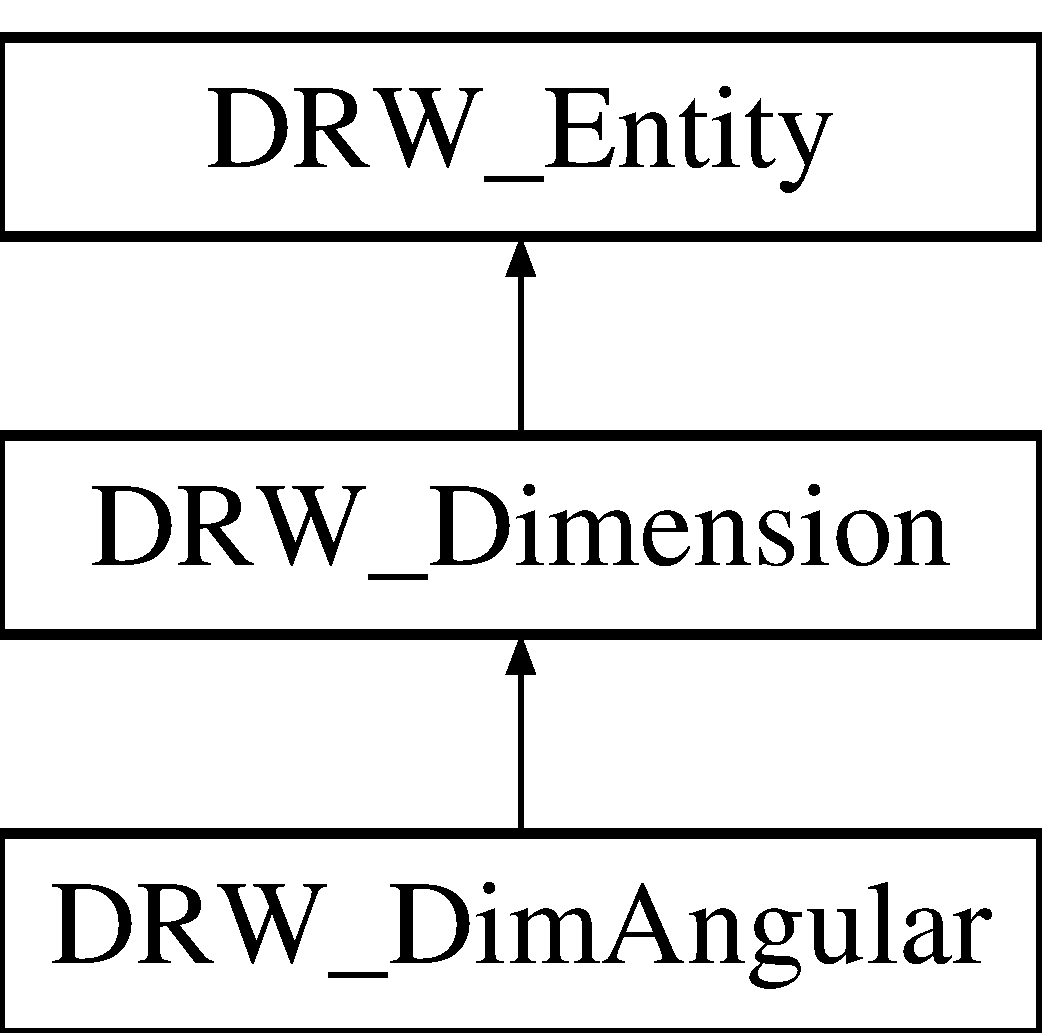
\includegraphics[height=3.000000cm]{dc/d8c/class_d_r_w___dim_angular}
\end{center}
\end{figure}
\subsection*{Public Member Functions}
\begin{DoxyCompactItemize}
\item 
\hyperlink{class_d_r_w___coord}{D\+R\+W\+\_\+\+Coord} \hyperlink{class_d_r_w___dim_angular_a19fd08973bf1c998d9c8d2ddec103d79}{get\+First\+Line1} () const 
\item 
\hyperlink{class_d_r_w___coord}{D\+R\+W\+\_\+\+Coord} \hyperlink{class_d_r_w___dim_angular_a7051a60adc2f98313877075088940c6b}{get\+First\+Line2} () const 
\item 
\hyperlink{class_d_r_w___coord}{D\+R\+W\+\_\+\+Coord} \hyperlink{class_d_r_w___dim_angular_a1733492e6857d946b5c9b1945b87227f}{get\+Second\+Line1} () const 
\item 
\hyperlink{class_d_r_w___coord}{D\+R\+W\+\_\+\+Coord} \hyperlink{class_d_r_w___dim_angular_aa242db6a477a20bb091bd3f2155b82f5}{get\+Second\+Line2} () const 
\item 
\hyperlink{class_d_r_w___coord}{D\+R\+W\+\_\+\+Coord} \hyperlink{class_d_r_w___dim_angular_a88ffb9c391ee06de48555a8defbbe732}{get\+Dim\+Point} () const 
\end{DoxyCompactItemize}
\subsection*{Additional Inherited Members}


\subsection{Detailed Description}
Class to handle angular dimension entity. 

Class to handle angular dimension entity \begin{DoxyAuthor}{Author}
Rallaz 
\end{DoxyAuthor}


\subsection{Member Function Documentation}
\hypertarget{class_d_r_w___dim_angular_a88ffb9c391ee06de48555a8defbbe732}{}\index{D\+R\+W\+\_\+\+Dim\+Angular@{D\+R\+W\+\_\+\+Dim\+Angular}!get\+Dim\+Point@{get\+Dim\+Point}}
\index{get\+Dim\+Point@{get\+Dim\+Point}!D\+R\+W\+\_\+\+Dim\+Angular@{D\+R\+W\+\_\+\+Dim\+Angular}}
\subsubsection[{get\+Dim\+Point}]{\setlength{\rightskip}{0pt plus 5cm}{\bf D\+R\+W\+\_\+\+Coord} D\+R\+W\+\_\+\+Dim\+Angular\+::get\+Dim\+Point (
\begin{DoxyParamCaption}
{}
\end{DoxyParamCaption}
) const\hspace{0.3cm}{\ttfamily [inline]}}\label{class_d_r_w___dim_angular_a88ffb9c391ee06de48555a8defbbe732}
Dimension definition point, code 16, 26 \& 36 \hypertarget{class_d_r_w___dim_angular_a19fd08973bf1c998d9c8d2ddec103d79}{}\index{D\+R\+W\+\_\+\+Dim\+Angular@{D\+R\+W\+\_\+\+Dim\+Angular}!get\+First\+Line1@{get\+First\+Line1}}
\index{get\+First\+Line1@{get\+First\+Line1}!D\+R\+W\+\_\+\+Dim\+Angular@{D\+R\+W\+\_\+\+Dim\+Angular}}
\subsubsection[{get\+First\+Line1}]{\setlength{\rightskip}{0pt plus 5cm}{\bf D\+R\+W\+\_\+\+Coord} D\+R\+W\+\_\+\+Dim\+Angular\+::get\+First\+Line1 (
\begin{DoxyParamCaption}
{}
\end{DoxyParamCaption}
) const\hspace{0.3cm}{\ttfamily [inline]}}\label{class_d_r_w___dim_angular_a19fd08973bf1c998d9c8d2ddec103d79}
Definition point line 1-\/1, code 13, 23 \& 33 \hypertarget{class_d_r_w___dim_angular_a7051a60adc2f98313877075088940c6b}{}\index{D\+R\+W\+\_\+\+Dim\+Angular@{D\+R\+W\+\_\+\+Dim\+Angular}!get\+First\+Line2@{get\+First\+Line2}}
\index{get\+First\+Line2@{get\+First\+Line2}!D\+R\+W\+\_\+\+Dim\+Angular@{D\+R\+W\+\_\+\+Dim\+Angular}}
\subsubsection[{get\+First\+Line2}]{\setlength{\rightskip}{0pt plus 5cm}{\bf D\+R\+W\+\_\+\+Coord} D\+R\+W\+\_\+\+Dim\+Angular\+::get\+First\+Line2 (
\begin{DoxyParamCaption}
{}
\end{DoxyParamCaption}
) const\hspace{0.3cm}{\ttfamily [inline]}}\label{class_d_r_w___dim_angular_a7051a60adc2f98313877075088940c6b}
Definition point line 1-\/2, code 14, 24 \& 34 \hypertarget{class_d_r_w___dim_angular_a1733492e6857d946b5c9b1945b87227f}{}\index{D\+R\+W\+\_\+\+Dim\+Angular@{D\+R\+W\+\_\+\+Dim\+Angular}!get\+Second\+Line1@{get\+Second\+Line1}}
\index{get\+Second\+Line1@{get\+Second\+Line1}!D\+R\+W\+\_\+\+Dim\+Angular@{D\+R\+W\+\_\+\+Dim\+Angular}}
\subsubsection[{get\+Second\+Line1}]{\setlength{\rightskip}{0pt plus 5cm}{\bf D\+R\+W\+\_\+\+Coord} D\+R\+W\+\_\+\+Dim\+Angular\+::get\+Second\+Line1 (
\begin{DoxyParamCaption}
{}
\end{DoxyParamCaption}
) const\hspace{0.3cm}{\ttfamily [inline]}}\label{class_d_r_w___dim_angular_a1733492e6857d946b5c9b1945b87227f}
Definition point line 2-\/1, code 15, 25 \& 35 \hypertarget{class_d_r_w___dim_angular_aa242db6a477a20bb091bd3f2155b82f5}{}\index{D\+R\+W\+\_\+\+Dim\+Angular@{D\+R\+W\+\_\+\+Dim\+Angular}!get\+Second\+Line2@{get\+Second\+Line2}}
\index{get\+Second\+Line2@{get\+Second\+Line2}!D\+R\+W\+\_\+\+Dim\+Angular@{D\+R\+W\+\_\+\+Dim\+Angular}}
\subsubsection[{get\+Second\+Line2}]{\setlength{\rightskip}{0pt plus 5cm}{\bf D\+R\+W\+\_\+\+Coord} D\+R\+W\+\_\+\+Dim\+Angular\+::get\+Second\+Line2 (
\begin{DoxyParamCaption}
{}
\end{DoxyParamCaption}
) const\hspace{0.3cm}{\ttfamily [inline]}}\label{class_d_r_w___dim_angular_aa242db6a477a20bb091bd3f2155b82f5}
Definition point line 2-\/2, code 10, 20 \& 30 

The documentation for this class was generated from the following file\+:\begin{DoxyCompactItemize}
\item 
src/drw\+\_\+entities.\+h\end{DoxyCompactItemize}

\hypertarget{class_d_r_w___dim_angular3p}{}\section{D\+R\+W\+\_\+\+Dim\+Angular3p Class Reference}
\label{class_d_r_w___dim_angular3p}\index{D\+R\+W\+\_\+\+Dim\+Angular3p@{D\+R\+W\+\_\+\+Dim\+Angular3p}}


Class to handle angular 3p dimension entity.  




{\ttfamily \#include $<$drw\+\_\+entities.\+h$>$}

Inheritance diagram for D\+R\+W\+\_\+\+Dim\+Angular3p\+:\begin{figure}[H]
\begin{center}
\leavevmode
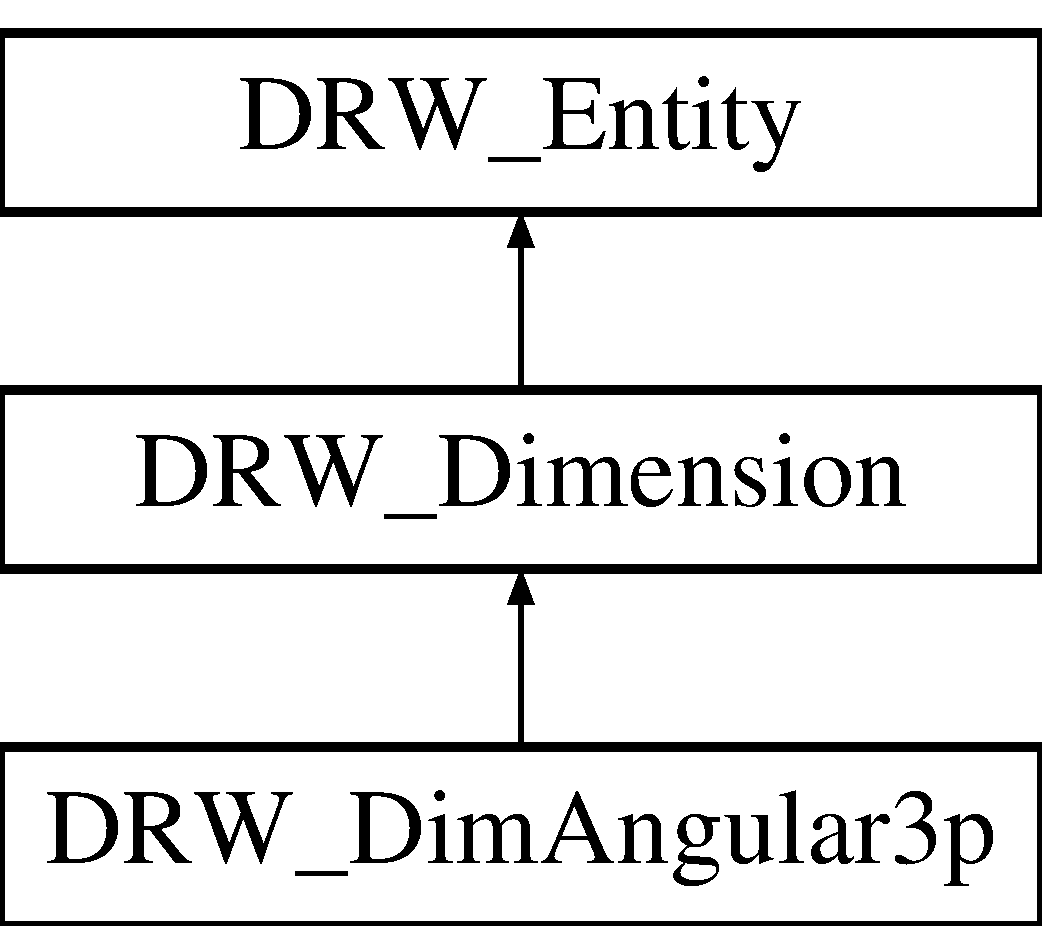
\includegraphics[height=3.000000cm]{d3/d32/class_d_r_w___dim_angular3p}
\end{center}
\end{figure}
\subsection*{Public Member Functions}
\begin{DoxyCompactItemize}
\item 
\hyperlink{class_d_r_w___coord}{D\+R\+W\+\_\+\+Coord} \hyperlink{class_d_r_w___dim_angular3p_a4b103b2e28a3f942f105118a84fffbb4}{get\+First\+Line} () const 
\item 
\hyperlink{class_d_r_w___coord}{D\+R\+W\+\_\+\+Coord} \hyperlink{class_d_r_w___dim_angular3p_aa240abbba2c8ce180e23c93e29ec604e}{get\+Second\+Line} () const 
\item 
\hyperlink{class_d_r_w___coord}{D\+R\+W\+\_\+\+Coord} \hyperlink{class_d_r_w___dim_angular3p_a331a4f869b667c46405c066eb819669e}{get\+Vertex\+Point} () const 
\item 
\hyperlink{class_d_r_w___coord}{D\+R\+W\+\_\+\+Coord} \hyperlink{class_d_r_w___dim_angular3p_abb2ea0c545d83aafbcc2d58b9ba959be}{get\+Dim\+Point} () const 
\end{DoxyCompactItemize}
\subsection*{Additional Inherited Members}


\subsection{Detailed Description}
Class to handle angular 3p dimension entity. 

Class to handle angular 3p dimension entity \begin{DoxyAuthor}{Author}
Rallaz 
\end{DoxyAuthor}


\subsection{Member Function Documentation}
\hypertarget{class_d_r_w___dim_angular3p_abb2ea0c545d83aafbcc2d58b9ba959be}{}\index{D\+R\+W\+\_\+\+Dim\+Angular3p@{D\+R\+W\+\_\+\+Dim\+Angular3p}!get\+Dim\+Point@{get\+Dim\+Point}}
\index{get\+Dim\+Point@{get\+Dim\+Point}!D\+R\+W\+\_\+\+Dim\+Angular3p@{D\+R\+W\+\_\+\+Dim\+Angular3p}}
\subsubsection[{get\+Dim\+Point}]{\setlength{\rightskip}{0pt plus 5cm}{\bf D\+R\+W\+\_\+\+Coord} D\+R\+W\+\_\+\+Dim\+Angular3p\+::get\+Dim\+Point (
\begin{DoxyParamCaption}
{}
\end{DoxyParamCaption}
) const\hspace{0.3cm}{\ttfamily [inline]}}\label{class_d_r_w___dim_angular3p_abb2ea0c545d83aafbcc2d58b9ba959be}
Dimension definition point, code 10, 20 \& 30 \hypertarget{class_d_r_w___dim_angular3p_a4b103b2e28a3f942f105118a84fffbb4}{}\index{D\+R\+W\+\_\+\+Dim\+Angular3p@{D\+R\+W\+\_\+\+Dim\+Angular3p}!get\+First\+Line@{get\+First\+Line}}
\index{get\+First\+Line@{get\+First\+Line}!D\+R\+W\+\_\+\+Dim\+Angular3p@{D\+R\+W\+\_\+\+Dim\+Angular3p}}
\subsubsection[{get\+First\+Line}]{\setlength{\rightskip}{0pt plus 5cm}{\bf D\+R\+W\+\_\+\+Coord} D\+R\+W\+\_\+\+Dim\+Angular3p\+::get\+First\+Line (
\begin{DoxyParamCaption}
{}
\end{DoxyParamCaption}
) const\hspace{0.3cm}{\ttfamily [inline]}}\label{class_d_r_w___dim_angular3p_a4b103b2e28a3f942f105118a84fffbb4}
Definition point line 1, code 13, 23 \& 33 \hypertarget{class_d_r_w___dim_angular3p_aa240abbba2c8ce180e23c93e29ec604e}{}\index{D\+R\+W\+\_\+\+Dim\+Angular3p@{D\+R\+W\+\_\+\+Dim\+Angular3p}!get\+Second\+Line@{get\+Second\+Line}}
\index{get\+Second\+Line@{get\+Second\+Line}!D\+R\+W\+\_\+\+Dim\+Angular3p@{D\+R\+W\+\_\+\+Dim\+Angular3p}}
\subsubsection[{get\+Second\+Line}]{\setlength{\rightskip}{0pt plus 5cm}{\bf D\+R\+W\+\_\+\+Coord} D\+R\+W\+\_\+\+Dim\+Angular3p\+::get\+Second\+Line (
\begin{DoxyParamCaption}
{}
\end{DoxyParamCaption}
) const\hspace{0.3cm}{\ttfamily [inline]}}\label{class_d_r_w___dim_angular3p_aa240abbba2c8ce180e23c93e29ec604e}
Definition point line 2, code 14, 24 \& 34 \hypertarget{class_d_r_w___dim_angular3p_a331a4f869b667c46405c066eb819669e}{}\index{D\+R\+W\+\_\+\+Dim\+Angular3p@{D\+R\+W\+\_\+\+Dim\+Angular3p}!get\+Vertex\+Point@{get\+Vertex\+Point}}
\index{get\+Vertex\+Point@{get\+Vertex\+Point}!D\+R\+W\+\_\+\+Dim\+Angular3p@{D\+R\+W\+\_\+\+Dim\+Angular3p}}
\subsubsection[{get\+Vertex\+Point}]{\setlength{\rightskip}{0pt plus 5cm}{\bf D\+R\+W\+\_\+\+Coord} D\+R\+W\+\_\+\+Dim\+Angular3p\+::get\+Vertex\+Point (
\begin{DoxyParamCaption}
{}
\end{DoxyParamCaption}
) const\hspace{0.3cm}{\ttfamily [inline]}}\label{class_d_r_w___dim_angular3p_a331a4f869b667c46405c066eb819669e}
Vertex point, code 15, 25 \& 35 

The documentation for this class was generated from the following file\+:\begin{DoxyCompactItemize}
\item 
src/drw\+\_\+entities.\+h\end{DoxyCompactItemize}

\hypertarget{class_d_r_w___dim_diametric}{}\section{D\+R\+W\+\_\+\+Dim\+Diametric Class Reference}
\label{class_d_r_w___dim_diametric}\index{D\+R\+W\+\_\+\+Dim\+Diametric@{D\+R\+W\+\_\+\+Dim\+Diametric}}


Class to handle radial dimension entity.  




{\ttfamily \#include $<$drw\+\_\+entities.\+h$>$}

Inheritance diagram for D\+R\+W\+\_\+\+Dim\+Diametric\+:\begin{figure}[H]
\begin{center}
\leavevmode
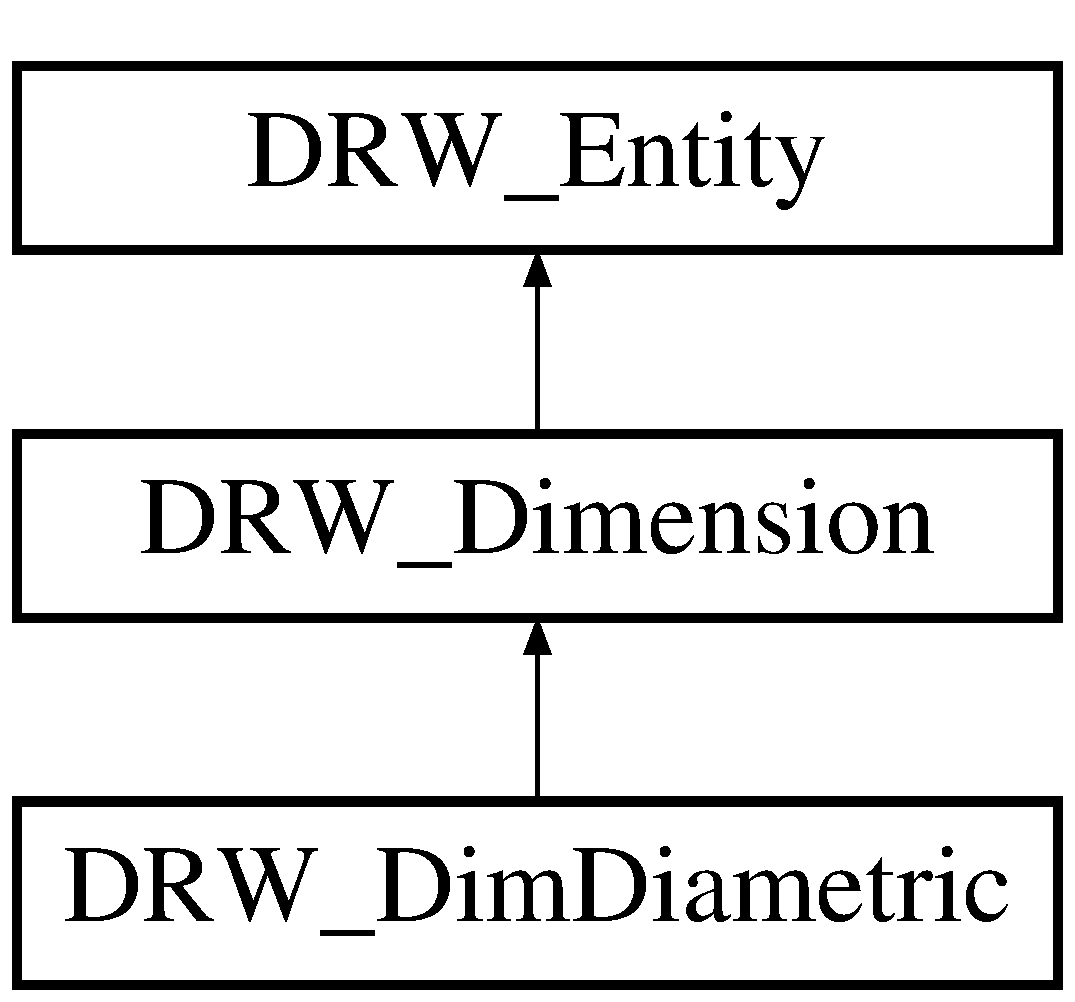
\includegraphics[height=3.000000cm]{d6/d19/class_d_r_w___dim_diametric}
\end{center}
\end{figure}
\subsection*{Public Member Functions}
\begin{DoxyCompactItemize}
\item 
\hyperlink{class_d_r_w___coord}{D\+R\+W\+\_\+\+Coord} \hyperlink{class_d_r_w___dim_diametric_accc66955a0cfcd75b11c68bebe310d3e}{get\+Diameter1\+Point} () const 
\item 
\hyperlink{class_d_r_w___coord}{D\+R\+W\+\_\+\+Coord} \hyperlink{class_d_r_w___dim_diametric_a9228e293ee74e3b70b32189c29de322c}{get\+Diameter2\+Point} () const 
\item 
double \hyperlink{class_d_r_w___dim_diametric_a1196c1df8bea7de9a9a89c158474cb48}{get\+Leader\+Length} () const 
\end{DoxyCompactItemize}
\subsection*{Additional Inherited Members}


\subsection{Detailed Description}
Class to handle radial dimension entity. 

Class to handle aligned, linear or rotated dimension entity \begin{DoxyAuthor}{Author}
Rallaz 
\end{DoxyAuthor}


\subsection{Member Function Documentation}
\hypertarget{class_d_r_w___dim_diametric_accc66955a0cfcd75b11c68bebe310d3e}{}\index{D\+R\+W\+\_\+\+Dim\+Diametric@{D\+R\+W\+\_\+\+Dim\+Diametric}!get\+Diameter1\+Point@{get\+Diameter1\+Point}}
\index{get\+Diameter1\+Point@{get\+Diameter1\+Point}!D\+R\+W\+\_\+\+Dim\+Diametric@{D\+R\+W\+\_\+\+Dim\+Diametric}}
\subsubsection[{get\+Diameter1\+Point}]{\setlength{\rightskip}{0pt plus 5cm}{\bf D\+R\+W\+\_\+\+Coord} D\+R\+W\+\_\+\+Dim\+Diametric\+::get\+Diameter1\+Point (
\begin{DoxyParamCaption}
{}
\end{DoxyParamCaption}
) const\hspace{0.3cm}{\ttfamily [inline]}}\label{class_d_r_w___dim_diametric_accc66955a0cfcd75b11c68bebe310d3e}
First definition point for diameter, code 15, 25 \& 35 \hypertarget{class_d_r_w___dim_diametric_a9228e293ee74e3b70b32189c29de322c}{}\index{D\+R\+W\+\_\+\+Dim\+Diametric@{D\+R\+W\+\_\+\+Dim\+Diametric}!get\+Diameter2\+Point@{get\+Diameter2\+Point}}
\index{get\+Diameter2\+Point@{get\+Diameter2\+Point}!D\+R\+W\+\_\+\+Dim\+Diametric@{D\+R\+W\+\_\+\+Dim\+Diametric}}
\subsubsection[{get\+Diameter2\+Point}]{\setlength{\rightskip}{0pt plus 5cm}{\bf D\+R\+W\+\_\+\+Coord} D\+R\+W\+\_\+\+Dim\+Diametric\+::get\+Diameter2\+Point (
\begin{DoxyParamCaption}
{}
\end{DoxyParamCaption}
) const\hspace{0.3cm}{\ttfamily [inline]}}\label{class_d_r_w___dim_diametric_a9228e293ee74e3b70b32189c29de322c}
Oposite point for diameter, code 10, 20 \& 30 \hypertarget{class_d_r_w___dim_diametric_a1196c1df8bea7de9a9a89c158474cb48}{}\index{D\+R\+W\+\_\+\+Dim\+Diametric@{D\+R\+W\+\_\+\+Dim\+Diametric}!get\+Leader\+Length@{get\+Leader\+Length}}
\index{get\+Leader\+Length@{get\+Leader\+Length}!D\+R\+W\+\_\+\+Dim\+Diametric@{D\+R\+W\+\_\+\+Dim\+Diametric}}
\subsubsection[{get\+Leader\+Length}]{\setlength{\rightskip}{0pt plus 5cm}double D\+R\+W\+\_\+\+Dim\+Diametric\+::get\+Leader\+Length (
\begin{DoxyParamCaption}
{}
\end{DoxyParamCaption}
) const\hspace{0.3cm}{\ttfamily [inline]}}\label{class_d_r_w___dim_diametric_a1196c1df8bea7de9a9a89c158474cb48}
Leader length, code 40 

The documentation for this class was generated from the following file\+:\begin{DoxyCompactItemize}
\item 
src/drw\+\_\+entities.\+h\end{DoxyCompactItemize}

\hypertarget{class_d_r_w___dimension}{}\section{D\+R\+W\+\_\+\+Dimension Class Reference}
\label{class_d_r_w___dimension}\index{D\+R\+W\+\_\+\+Dimension@{D\+R\+W\+\_\+\+Dimension}}


Base class for dimension entity.  




{\ttfamily \#include $<$drw\+\_\+entities.\+h$>$}

Inheritance diagram for D\+R\+W\+\_\+\+Dimension\+:\begin{figure}[H]
\begin{center}
\leavevmode
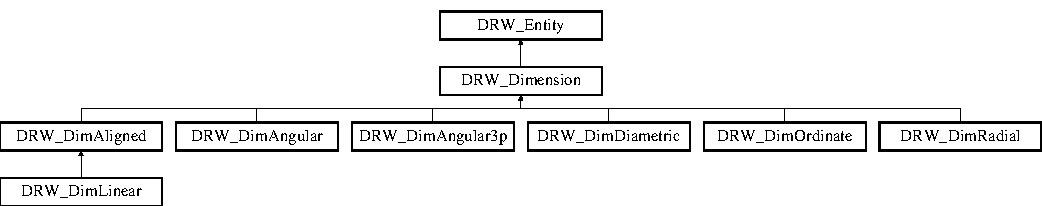
\includegraphics[height=2.765432cm]{df/d1d/class_d_r_w___dimension}
\end{center}
\end{figure}
\subsection*{Public Member Functions}
\begin{DoxyCompactItemize}
\item 
\hyperlink{class_d_r_w___coord}{D\+R\+W\+\_\+\+Coord} \hyperlink{class_d_r_w___dimension_aff7c5b5035b520428c2a0c181f7cb102}{get\+Def\+Point} () const 
\item 
\hyperlink{class_d_r_w___coord}{D\+R\+W\+\_\+\+Coord} \hyperlink{class_d_r_w___dimension_aa7dcaa119dfc8aaacdf093067ac5a781}{get\+Text\+Point} () const 
\item 
std\+::string \hyperlink{class_d_r_w___dimension_a617836523c243ac0cec7871dcee13518}{get\+Style} () const 
\item 
int \hyperlink{class_d_r_w___dimension_ac4423a75a6bf64525e096fe72938bfd7}{get\+Align} () const 
\item 
int \hyperlink{class_d_r_w___dimension_a5774fd11d8745a32e6c2a94a697a3584}{get\+Text\+Line\+Style} () const 
\item 
std\+::string \hyperlink{class_d_r_w___dimension_a34b21f424946313158384673fb5bc885}{get\+Text} () const 
\item 
double \hyperlink{class_d_r_w___dimension_a92f00fef72a9f5de2058360f7ce4d518}{get\+Text\+Line\+Factor} () const 
\item 
double \hyperlink{class_d_r_w___dimension_afce2fe039bfbff29ef8dca9ab5d4d41c}{get\+Dir} () const 
\item 
\hyperlink{class_d_r_w___coord}{D\+R\+W\+\_\+\+Coord} \hyperlink{class_d_r_w___dimension_acbbe026791231ce980ad2adcf0a259c2}{get\+Extrusion} ()
\item 
std\+::string \hyperlink{class_d_r_w___dimension_aece5c640691b5ee65674e852ea2ea812}{get\+Name} ()
\end{DoxyCompactItemize}
\subsection*{Public Attributes}
\begin{DoxyCompactItemize}
\item 
int \hyperlink{class_d_r_w___dimension_ad3af7cb327656cb2c1c33a00d26ed933}{type}
\end{DoxyCompactItemize}
\subsection*{Protected Member Functions}
\begin{DoxyCompactItemize}
\item 
double \hyperlink{class_d_r_w___dimension_ae45501f2cad8bdcd9be874ff4f05749b}{get\+An50} () const 
\item 
double \hyperlink{class_d_r_w___dimension_a36825b8bb477ec416d20a68d3cc5d54e}{get\+Ob52} () const 
\item 
double \hyperlink{class_d_r_w___dimension_a6d8226ab5f019e2cd2f9a46c4fa7cade}{get\+Ra40} () const 
\end{DoxyCompactItemize}
\subsection*{Private Attributes}
\begin{DoxyCompactItemize}
\item 
std\+::string \hyperlink{class_d_r_w___dimension_a1aa04de9a7c3db31c2bcccda811eeb6b}{name}
\item 
\hyperlink{class_d_r_w___coord}{D\+R\+W\+\_\+\+Coord} \hyperlink{class_d_r_w___dimension_a1f00cdbce7d5d7139578ded6fe44f336}{def\+Point}
\item 
\hyperlink{class_d_r_w___coord}{D\+R\+W\+\_\+\+Coord} \hyperlink{class_d_r_w___dimension_a166186e4b2b8e23b476e2c1b69878c49}{text\+Point}
\item 
U\+T\+F8\+S\+T\+R\+I\+N\+G \hyperlink{class_d_r_w___dimension_a0e7e8ed05c8bf34019ce2594075611cd}{text}
\item 
U\+T\+F8\+S\+T\+R\+I\+N\+G \hyperlink{class_d_r_w___dimension_af781a0d7108a2caf9642b4a7cc79b1fb}{style}
\item 
int \hyperlink{class_d_r_w___dimension_ab4c71bb988fda882c0a5a7d27049c66d}{align}
\item 
int \hyperlink{class_d_r_w___dimension_a3915235284c71e9e87ec6c4c18b95449}{linesty}
\item 
double \hyperlink{class_d_r_w___dimension_a629153fb6c846e1b2d8dabf6e32956d1}{linefactor}
\item 
double \hyperlink{class_d_r_w___dimension_a57b01df4f4f27aafc4adb56fed4b979d}{rot}
\item 
\hyperlink{class_d_r_w___coord}{D\+R\+W\+\_\+\+Coord} \hyperlink{class_d_r_w___dimension_a205674ec560ace6c57f14332a8992e2d}{ext\+Point}
\item 
\hyperlink{class_d_r_w___coord}{D\+R\+W\+\_\+\+Coord} \hyperlink{class_d_r_w___dimension_a62895c83fdbe0acf0d94db2bf3716711}{clone\+Point}
\item 
\hyperlink{class_d_r_w___coord}{D\+R\+W\+\_\+\+Coord} \hyperlink{class_d_r_w___dimension_acce64719064a0d64a19a715c6f42a6a5}{def1}
\item 
\hyperlink{class_d_r_w___coord}{D\+R\+W\+\_\+\+Coord} \hyperlink{class_d_r_w___dimension_a8372d63a865ea08dc547e3ee774abb0c}{def2}
\item 
double \hyperlink{class_d_r_w___dimension_a743d646215e437f004e41427a0c306b5}{angle}
\item 
double \hyperlink{class_d_r_w___dimension_a2f0983aa339252883ae945baad31cf34}{oblique}
\item 
\hyperlink{class_d_r_w___coord}{D\+R\+W\+\_\+\+Coord} \hyperlink{class_d_r_w___dimension_af4a22d548b9618d76cd57583d90eeb12}{circle\+Point}
\item 
\hyperlink{class_d_r_w___coord}{D\+R\+W\+\_\+\+Coord} \hyperlink{class_d_r_w___dimension_ac30d5ff5140020f86f48de68ccd2b907}{arc\+Point}
\item 
double \hyperlink{class_d_r_w___dimension_accab6e5384d68c63b458d364fa9bf0e3}{length}
\end{DoxyCompactItemize}
\subsection*{Friends}
\begin{DoxyCompactItemize}
\item 
\hypertarget{class_d_r_w___dimension_a7f080e77e5112f8364c61b97387f8ee2}{}class {\bfseries dxf\+R\+W}\label{class_d_r_w___dimension_a7f080e77e5112f8364c61b97387f8ee2}

\end{DoxyCompactItemize}


\subsection{Detailed Description}
Base class for dimension entity. 

Base class for dimension entity \begin{DoxyAuthor}{Author}
Rallaz 
\end{DoxyAuthor}


\subsection{Member Function Documentation}
\hypertarget{class_d_r_w___dimension_ac4423a75a6bf64525e096fe72938bfd7}{}\index{D\+R\+W\+\_\+\+Dimension@{D\+R\+W\+\_\+\+Dimension}!get\+Align@{get\+Align}}
\index{get\+Align@{get\+Align}!D\+R\+W\+\_\+\+Dimension@{D\+R\+W\+\_\+\+Dimension}}
\subsubsection[{get\+Align}]{\setlength{\rightskip}{0pt plus 5cm}int D\+R\+W\+\_\+\+Dimension\+::get\+Align (
\begin{DoxyParamCaption}
{}
\end{DoxyParamCaption}
) const\hspace{0.3cm}{\ttfamily [inline]}}\label{class_d_r_w___dimension_ac4423a75a6bf64525e096fe72938bfd7}
attachment point, code 71 \hypertarget{class_d_r_w___dimension_ae45501f2cad8bdcd9be874ff4f05749b}{}\index{D\+R\+W\+\_\+\+Dimension@{D\+R\+W\+\_\+\+Dimension}!get\+An50@{get\+An50}}
\index{get\+An50@{get\+An50}!D\+R\+W\+\_\+\+Dimension@{D\+R\+W\+\_\+\+Dimension}}
\subsubsection[{get\+An50}]{\setlength{\rightskip}{0pt plus 5cm}double D\+R\+W\+\_\+\+Dimension\+::get\+An50 (
\begin{DoxyParamCaption}
{}
\end{DoxyParamCaption}
) const\hspace{0.3cm}{\ttfamily [inline]}, {\ttfamily [protected]}}\label{class_d_r_w___dimension_ae45501f2cad8bdcd9be874ff4f05749b}
Angle of rotated, horizontal, or vertical dimensions, code 50 \hypertarget{class_d_r_w___dimension_aff7c5b5035b520428c2a0c181f7cb102}{}\index{D\+R\+W\+\_\+\+Dimension@{D\+R\+W\+\_\+\+Dimension}!get\+Def\+Point@{get\+Def\+Point}}
\index{get\+Def\+Point@{get\+Def\+Point}!D\+R\+W\+\_\+\+Dimension@{D\+R\+W\+\_\+\+Dimension}}
\subsubsection[{get\+Def\+Point}]{\setlength{\rightskip}{0pt plus 5cm}{\bf D\+R\+W\+\_\+\+Coord} D\+R\+W\+\_\+\+Dimension\+::get\+Def\+Point (
\begin{DoxyParamCaption}
{}
\end{DoxyParamCaption}
) const\hspace{0.3cm}{\ttfamily [inline]}}\label{class_d_r_w___dimension_aff7c5b5035b520428c2a0c181f7cb102}
Definition point, code 10, 20 \& 30 \hypertarget{class_d_r_w___dimension_afce2fe039bfbff29ef8dca9ab5d4d41c}{}\index{D\+R\+W\+\_\+\+Dimension@{D\+R\+W\+\_\+\+Dimension}!get\+Dir@{get\+Dir}}
\index{get\+Dir@{get\+Dir}!D\+R\+W\+\_\+\+Dimension@{D\+R\+W\+\_\+\+Dimension}}
\subsubsection[{get\+Dir}]{\setlength{\rightskip}{0pt plus 5cm}double D\+R\+W\+\_\+\+Dimension\+::get\+Dir (
\begin{DoxyParamCaption}
{}
\end{DoxyParamCaption}
) const\hspace{0.3cm}{\ttfamily [inline]}}\label{class_d_r_w___dimension_afce2fe039bfbff29ef8dca9ab5d4d41c}
rotation angle of the dimension text, code 53 (optional) default 0 \hypertarget{class_d_r_w___dimension_acbbe026791231ce980ad2adcf0a259c2}{}\index{D\+R\+W\+\_\+\+Dimension@{D\+R\+W\+\_\+\+Dimension}!get\+Extrusion@{get\+Extrusion}}
\index{get\+Extrusion@{get\+Extrusion}!D\+R\+W\+\_\+\+Dimension@{D\+R\+W\+\_\+\+Dimension}}
\subsubsection[{get\+Extrusion}]{\setlength{\rightskip}{0pt plus 5cm}{\bf D\+R\+W\+\_\+\+Coord} D\+R\+W\+\_\+\+Dimension\+::get\+Extrusion (
\begin{DoxyParamCaption}
{}
\end{DoxyParamCaption}
)\hspace{0.3cm}{\ttfamily [inline]}}\label{class_d_r_w___dimension_acbbe026791231ce980ad2adcf0a259c2}
extrusion, code 210, 220 \& 230 \hypertarget{class_d_r_w___dimension_aece5c640691b5ee65674e852ea2ea812}{}\index{D\+R\+W\+\_\+\+Dimension@{D\+R\+W\+\_\+\+Dimension}!get\+Name@{get\+Name}}
\index{get\+Name@{get\+Name}!D\+R\+W\+\_\+\+Dimension@{D\+R\+W\+\_\+\+Dimension}}
\subsubsection[{get\+Name}]{\setlength{\rightskip}{0pt plus 5cm}std\+::string D\+R\+W\+\_\+\+Dimension\+::get\+Name (
\begin{DoxyParamCaption}
{}
\end{DoxyParamCaption}
)\hspace{0.3cm}{\ttfamily [inline]}}\label{class_d_r_w___dimension_aece5c640691b5ee65674e852ea2ea812}
Name of the block that contains the entities, code 2 \hypertarget{class_d_r_w___dimension_a36825b8bb477ec416d20a68d3cc5d54e}{}\index{D\+R\+W\+\_\+\+Dimension@{D\+R\+W\+\_\+\+Dimension}!get\+Ob52@{get\+Ob52}}
\index{get\+Ob52@{get\+Ob52}!D\+R\+W\+\_\+\+Dimension@{D\+R\+W\+\_\+\+Dimension}}
\subsubsection[{get\+Ob52}]{\setlength{\rightskip}{0pt plus 5cm}double D\+R\+W\+\_\+\+Dimension\+::get\+Ob52 (
\begin{DoxyParamCaption}
{}
\end{DoxyParamCaption}
) const\hspace{0.3cm}{\ttfamily [inline]}, {\ttfamily [protected]}}\label{class_d_r_w___dimension_a36825b8bb477ec416d20a68d3cc5d54e}
oblique angle, code 52 \hypertarget{class_d_r_w___dimension_a6d8226ab5f019e2cd2f9a46c4fa7cade}{}\index{D\+R\+W\+\_\+\+Dimension@{D\+R\+W\+\_\+\+Dimension}!get\+Ra40@{get\+Ra40}}
\index{get\+Ra40@{get\+Ra40}!D\+R\+W\+\_\+\+Dimension@{D\+R\+W\+\_\+\+Dimension}}
\subsubsection[{get\+Ra40}]{\setlength{\rightskip}{0pt plus 5cm}double D\+R\+W\+\_\+\+Dimension\+::get\+Ra40 (
\begin{DoxyParamCaption}
{}
\end{DoxyParamCaption}
) const\hspace{0.3cm}{\ttfamily [inline]}, {\ttfamily [protected]}}\label{class_d_r_w___dimension_a6d8226ab5f019e2cd2f9a46c4fa7cade}
Leader length, code 40 \hypertarget{class_d_r_w___dimension_a617836523c243ac0cec7871dcee13518}{}\index{D\+R\+W\+\_\+\+Dimension@{D\+R\+W\+\_\+\+Dimension}!get\+Style@{get\+Style}}
\index{get\+Style@{get\+Style}!D\+R\+W\+\_\+\+Dimension@{D\+R\+W\+\_\+\+Dimension}}
\subsubsection[{get\+Style}]{\setlength{\rightskip}{0pt plus 5cm}std\+::string D\+R\+W\+\_\+\+Dimension\+::get\+Style (
\begin{DoxyParamCaption}
{}
\end{DoxyParamCaption}
) const\hspace{0.3cm}{\ttfamily [inline]}}\label{class_d_r_w___dimension_a617836523c243ac0cec7871dcee13518}
Dimension style, code 3 \hypertarget{class_d_r_w___dimension_a34b21f424946313158384673fb5bc885}{}\index{D\+R\+W\+\_\+\+Dimension@{D\+R\+W\+\_\+\+Dimension}!get\+Text@{get\+Text}}
\index{get\+Text@{get\+Text}!D\+R\+W\+\_\+\+Dimension@{D\+R\+W\+\_\+\+Dimension}}
\subsubsection[{get\+Text}]{\setlength{\rightskip}{0pt plus 5cm}std\+::string D\+R\+W\+\_\+\+Dimension\+::get\+Text (
\begin{DoxyParamCaption}
{}
\end{DoxyParamCaption}
) const\hspace{0.3cm}{\ttfamily [inline]}}\label{class_d_r_w___dimension_a34b21f424946313158384673fb5bc885}
Dimension text explicitly entered by the user, code 1 \hypertarget{class_d_r_w___dimension_a92f00fef72a9f5de2058360f7ce4d518}{}\index{D\+R\+W\+\_\+\+Dimension@{D\+R\+W\+\_\+\+Dimension}!get\+Text\+Line\+Factor@{get\+Text\+Line\+Factor}}
\index{get\+Text\+Line\+Factor@{get\+Text\+Line\+Factor}!D\+R\+W\+\_\+\+Dimension@{D\+R\+W\+\_\+\+Dimension}}
\subsubsection[{get\+Text\+Line\+Factor}]{\setlength{\rightskip}{0pt plus 5cm}double D\+R\+W\+\_\+\+Dimension\+::get\+Text\+Line\+Factor (
\begin{DoxyParamCaption}
{}
\end{DoxyParamCaption}
) const\hspace{0.3cm}{\ttfamily [inline]}}\label{class_d_r_w___dimension_a92f00fef72a9f5de2058360f7ce4d518}
Dimension text line spacing factor, code 41, default 1? \hypertarget{class_d_r_w___dimension_a5774fd11d8745a32e6c2a94a697a3584}{}\index{D\+R\+W\+\_\+\+Dimension@{D\+R\+W\+\_\+\+Dimension}!get\+Text\+Line\+Style@{get\+Text\+Line\+Style}}
\index{get\+Text\+Line\+Style@{get\+Text\+Line\+Style}!D\+R\+W\+\_\+\+Dimension@{D\+R\+W\+\_\+\+Dimension}}
\subsubsection[{get\+Text\+Line\+Style}]{\setlength{\rightskip}{0pt plus 5cm}int D\+R\+W\+\_\+\+Dimension\+::get\+Text\+Line\+Style (
\begin{DoxyParamCaption}
{}
\end{DoxyParamCaption}
) const\hspace{0.3cm}{\ttfamily [inline]}}\label{class_d_r_w___dimension_a5774fd11d8745a32e6c2a94a697a3584}
Dimension text line spacing style, code 72, default 1 \hypertarget{class_d_r_w___dimension_aa7dcaa119dfc8aaacdf093067ac5a781}{}\index{D\+R\+W\+\_\+\+Dimension@{D\+R\+W\+\_\+\+Dimension}!get\+Text\+Point@{get\+Text\+Point}}
\index{get\+Text\+Point@{get\+Text\+Point}!D\+R\+W\+\_\+\+Dimension@{D\+R\+W\+\_\+\+Dimension}}
\subsubsection[{get\+Text\+Point}]{\setlength{\rightskip}{0pt plus 5cm}{\bf D\+R\+W\+\_\+\+Coord} D\+R\+W\+\_\+\+Dimension\+::get\+Text\+Point (
\begin{DoxyParamCaption}
{}
\end{DoxyParamCaption}
) const\hspace{0.3cm}{\ttfamily [inline]}}\label{class_d_r_w___dimension_aa7dcaa119dfc8aaacdf093067ac5a781}
Middle point of text, code 11, 21 \& 31 

\subsection{Member Data Documentation}
\hypertarget{class_d_r_w___dimension_ab4c71bb988fda882c0a5a7d27049c66d}{}\index{D\+R\+W\+\_\+\+Dimension@{D\+R\+W\+\_\+\+Dimension}!align@{align}}
\index{align@{align}!D\+R\+W\+\_\+\+Dimension@{D\+R\+W\+\_\+\+Dimension}}
\subsubsection[{align}]{\setlength{\rightskip}{0pt plus 5cm}int D\+R\+W\+\_\+\+Dimension\+::align\hspace{0.3cm}{\ttfamily [private]}}\label{class_d_r_w___dimension_ab4c71bb988fda882c0a5a7d27049c66d}
attachment point, code 71 \hypertarget{class_d_r_w___dimension_a743d646215e437f004e41427a0c306b5}{}\index{D\+R\+W\+\_\+\+Dimension@{D\+R\+W\+\_\+\+Dimension}!angle@{angle}}
\index{angle@{angle}!D\+R\+W\+\_\+\+Dimension@{D\+R\+W\+\_\+\+Dimension}}
\subsubsection[{angle}]{\setlength{\rightskip}{0pt plus 5cm}double D\+R\+W\+\_\+\+Dimension\+::angle\hspace{0.3cm}{\ttfamily [private]}}\label{class_d_r_w___dimension_a743d646215e437f004e41427a0c306b5}
Angle of rotated, horizontal, or vertical dimensions, code 50 \hypertarget{class_d_r_w___dimension_ac30d5ff5140020f86f48de68ccd2b907}{}\index{D\+R\+W\+\_\+\+Dimension@{D\+R\+W\+\_\+\+Dimension}!arc\+Point@{arc\+Point}}
\index{arc\+Point@{arc\+Point}!D\+R\+W\+\_\+\+Dimension@{D\+R\+W\+\_\+\+Dimension}}
\subsubsection[{arc\+Point}]{\setlength{\rightskip}{0pt plus 5cm}{\bf D\+R\+W\+\_\+\+Coord} D\+R\+W\+\_\+\+Dimension\+::arc\+Point\hspace{0.3cm}{\ttfamily [private]}}\label{class_d_r_w___dimension_ac30d5ff5140020f86f48de68ccd2b907}
Point defining dimension arc, x coordinate, code 16, 26 \& 36 (O\+C\+S) \hypertarget{class_d_r_w___dimension_af4a22d548b9618d76cd57583d90eeb12}{}\index{D\+R\+W\+\_\+\+Dimension@{D\+R\+W\+\_\+\+Dimension}!circle\+Point@{circle\+Point}}
\index{circle\+Point@{circle\+Point}!D\+R\+W\+\_\+\+Dimension@{D\+R\+W\+\_\+\+Dimension}}
\subsubsection[{circle\+Point}]{\setlength{\rightskip}{0pt plus 5cm}{\bf D\+R\+W\+\_\+\+Coord} D\+R\+W\+\_\+\+Dimension\+::circle\+Point\hspace{0.3cm}{\ttfamily [private]}}\label{class_d_r_w___dimension_af4a22d548b9618d76cd57583d90eeb12}
Definition point for diameter, radius \& angular dims code 15, 25 \& 35 (W\+C\+S) \hypertarget{class_d_r_w___dimension_a62895c83fdbe0acf0d94db2bf3716711}{}\index{D\+R\+W\+\_\+\+Dimension@{D\+R\+W\+\_\+\+Dimension}!clone\+Point@{clone\+Point}}
\index{clone\+Point@{clone\+Point}!D\+R\+W\+\_\+\+Dimension@{D\+R\+W\+\_\+\+Dimension}}
\subsubsection[{clone\+Point}]{\setlength{\rightskip}{0pt plus 5cm}{\bf D\+R\+W\+\_\+\+Coord} D\+R\+W\+\_\+\+Dimension\+::clone\+Point\hspace{0.3cm}{\ttfamily [private]}}\label{class_d_r_w___dimension_a62895c83fdbe0acf0d94db2bf3716711}
Insertion point for clones (Baseline \& Continue), code 12, 22 \& 32 (O\+C\+S) \hypertarget{class_d_r_w___dimension_acce64719064a0d64a19a715c6f42a6a5}{}\index{D\+R\+W\+\_\+\+Dimension@{D\+R\+W\+\_\+\+Dimension}!def1@{def1}}
\index{def1@{def1}!D\+R\+W\+\_\+\+Dimension@{D\+R\+W\+\_\+\+Dimension}}
\subsubsection[{def1}]{\setlength{\rightskip}{0pt plus 5cm}{\bf D\+R\+W\+\_\+\+Coord} D\+R\+W\+\_\+\+Dimension\+::def1\hspace{0.3cm}{\ttfamily [private]}}\label{class_d_r_w___dimension_acce64719064a0d64a19a715c6f42a6a5}
Definition point 1for linear \& angular, code 13, 23 \& 33 (W\+C\+S) \hypertarget{class_d_r_w___dimension_a8372d63a865ea08dc547e3ee774abb0c}{}\index{D\+R\+W\+\_\+\+Dimension@{D\+R\+W\+\_\+\+Dimension}!def2@{def2}}
\index{def2@{def2}!D\+R\+W\+\_\+\+Dimension@{D\+R\+W\+\_\+\+Dimension}}
\subsubsection[{def2}]{\setlength{\rightskip}{0pt plus 5cm}{\bf D\+R\+W\+\_\+\+Coord} D\+R\+W\+\_\+\+Dimension\+::def2\hspace{0.3cm}{\ttfamily [private]}}\label{class_d_r_w___dimension_a8372d63a865ea08dc547e3ee774abb0c}
Definition point 2, code 14, 24 \& 34 (W\+C\+S) \hypertarget{class_d_r_w___dimension_a1f00cdbce7d5d7139578ded6fe44f336}{}\index{D\+R\+W\+\_\+\+Dimension@{D\+R\+W\+\_\+\+Dimension}!def\+Point@{def\+Point}}
\index{def\+Point@{def\+Point}!D\+R\+W\+\_\+\+Dimension@{D\+R\+W\+\_\+\+Dimension}}
\subsubsection[{def\+Point}]{\setlength{\rightskip}{0pt plus 5cm}{\bf D\+R\+W\+\_\+\+Coord} D\+R\+W\+\_\+\+Dimension\+::def\+Point\hspace{0.3cm}{\ttfamily [private]}}\label{class_d_r_w___dimension_a1f00cdbce7d5d7139578ded6fe44f336}
definition point, code 10, 20 \& 30 (W\+C\+S) \hypertarget{class_d_r_w___dimension_a205674ec560ace6c57f14332a8992e2d}{}\index{D\+R\+W\+\_\+\+Dimension@{D\+R\+W\+\_\+\+Dimension}!ext\+Point@{ext\+Point}}
\index{ext\+Point@{ext\+Point}!D\+R\+W\+\_\+\+Dimension@{D\+R\+W\+\_\+\+Dimension}}
\subsubsection[{ext\+Point}]{\setlength{\rightskip}{0pt plus 5cm}{\bf D\+R\+W\+\_\+\+Coord} D\+R\+W\+\_\+\+Dimension\+::ext\+Point\hspace{0.3cm}{\ttfamily [private]}}\label{class_d_r_w___dimension_a205674ec560ace6c57f14332a8992e2d}
extrusion normal vector, code 210, 220 \& 230 \hypertarget{class_d_r_w___dimension_accab6e5384d68c63b458d364fa9bf0e3}{}\index{D\+R\+W\+\_\+\+Dimension@{D\+R\+W\+\_\+\+Dimension}!length@{length}}
\index{length@{length}!D\+R\+W\+\_\+\+Dimension@{D\+R\+W\+\_\+\+Dimension}}
\subsubsection[{length}]{\setlength{\rightskip}{0pt plus 5cm}double D\+R\+W\+\_\+\+Dimension\+::length\hspace{0.3cm}{\ttfamily [private]}}\label{class_d_r_w___dimension_accab6e5384d68c63b458d364fa9bf0e3}
Leader length, code 40 \hypertarget{class_d_r_w___dimension_a629153fb6c846e1b2d8dabf6e32956d1}{}\index{D\+R\+W\+\_\+\+Dimension@{D\+R\+W\+\_\+\+Dimension}!linefactor@{linefactor}}
\index{linefactor@{linefactor}!D\+R\+W\+\_\+\+Dimension@{D\+R\+W\+\_\+\+Dimension}}
\subsubsection[{linefactor}]{\setlength{\rightskip}{0pt plus 5cm}double D\+R\+W\+\_\+\+Dimension\+::linefactor\hspace{0.3cm}{\ttfamily [private]}}\label{class_d_r_w___dimension_a629153fb6c846e1b2d8dabf6e32956d1}
Dimension text line spacing factor, code 41, default 1? (value range 0.\+25 to 4.\+00 \hypertarget{class_d_r_w___dimension_a3915235284c71e9e87ec6c4c18b95449}{}\index{D\+R\+W\+\_\+\+Dimension@{D\+R\+W\+\_\+\+Dimension}!linesty@{linesty}}
\index{linesty@{linesty}!D\+R\+W\+\_\+\+Dimension@{D\+R\+W\+\_\+\+Dimension}}
\subsubsection[{linesty}]{\setlength{\rightskip}{0pt plus 5cm}int D\+R\+W\+\_\+\+Dimension\+::linesty\hspace{0.3cm}{\ttfamily [private]}}\label{class_d_r_w___dimension_a3915235284c71e9e87ec6c4c18b95449}
Dimension text line spacing style, code 72, default 1 \hypertarget{class_d_r_w___dimension_a1aa04de9a7c3db31c2bcccda811eeb6b}{}\index{D\+R\+W\+\_\+\+Dimension@{D\+R\+W\+\_\+\+Dimension}!name@{name}}
\index{name@{name}!D\+R\+W\+\_\+\+Dimension@{D\+R\+W\+\_\+\+Dimension}}
\subsubsection[{name}]{\setlength{\rightskip}{0pt plus 5cm}std\+::string D\+R\+W\+\_\+\+Dimension\+::name\hspace{0.3cm}{\ttfamily [private]}}\label{class_d_r_w___dimension_a1aa04de9a7c3db31c2bcccda811eeb6b}
Name of the block that contains the entities, code 2 \hypertarget{class_d_r_w___dimension_a2f0983aa339252883ae945baad31cf34}{}\index{D\+R\+W\+\_\+\+Dimension@{D\+R\+W\+\_\+\+Dimension}!oblique@{oblique}}
\index{oblique@{oblique}!D\+R\+W\+\_\+\+Dimension@{D\+R\+W\+\_\+\+Dimension}}
\subsubsection[{oblique}]{\setlength{\rightskip}{0pt plus 5cm}double D\+R\+W\+\_\+\+Dimension\+::oblique\hspace{0.3cm}{\ttfamily [private]}}\label{class_d_r_w___dimension_a2f0983aa339252883ae945baad31cf34}
oblique angle, code 52 \hypertarget{class_d_r_w___dimension_a57b01df4f4f27aafc4adb56fed4b979d}{}\index{D\+R\+W\+\_\+\+Dimension@{D\+R\+W\+\_\+\+Dimension}!rot@{rot}}
\index{rot@{rot}!D\+R\+W\+\_\+\+Dimension@{D\+R\+W\+\_\+\+Dimension}}
\subsubsection[{rot}]{\setlength{\rightskip}{0pt plus 5cm}double D\+R\+W\+\_\+\+Dimension\+::rot\hspace{0.3cm}{\ttfamily [private]}}\label{class_d_r_w___dimension_a57b01df4f4f27aafc4adb56fed4b979d}
rotation angle of the dimension text, code 53 \hypertarget{class_d_r_w___dimension_af781a0d7108a2caf9642b4a7cc79b1fb}{}\index{D\+R\+W\+\_\+\+Dimension@{D\+R\+W\+\_\+\+Dimension}!style@{style}}
\index{style@{style}!D\+R\+W\+\_\+\+Dimension@{D\+R\+W\+\_\+\+Dimension}}
\subsubsection[{style}]{\setlength{\rightskip}{0pt plus 5cm}U\+T\+F8\+S\+T\+R\+I\+N\+G D\+R\+W\+\_\+\+Dimension\+::style\hspace{0.3cm}{\ttfamily [private]}}\label{class_d_r_w___dimension_af781a0d7108a2caf9642b4a7cc79b1fb}
Dimension style, code 3 \hypertarget{class_d_r_w___dimension_a0e7e8ed05c8bf34019ce2594075611cd}{}\index{D\+R\+W\+\_\+\+Dimension@{D\+R\+W\+\_\+\+Dimension}!text@{text}}
\index{text@{text}!D\+R\+W\+\_\+\+Dimension@{D\+R\+W\+\_\+\+Dimension}}
\subsubsection[{text}]{\setlength{\rightskip}{0pt plus 5cm}U\+T\+F8\+S\+T\+R\+I\+N\+G D\+R\+W\+\_\+\+Dimension\+::text\hspace{0.3cm}{\ttfamily [private]}}\label{class_d_r_w___dimension_a0e7e8ed05c8bf34019ce2594075611cd}
Dimension text explicitly entered by the user, code 1 \hypertarget{class_d_r_w___dimension_a166186e4b2b8e23b476e2c1b69878c49}{}\index{D\+R\+W\+\_\+\+Dimension@{D\+R\+W\+\_\+\+Dimension}!text\+Point@{text\+Point}}
\index{text\+Point@{text\+Point}!D\+R\+W\+\_\+\+Dimension@{D\+R\+W\+\_\+\+Dimension}}
\subsubsection[{text\+Point}]{\setlength{\rightskip}{0pt plus 5cm}{\bf D\+R\+W\+\_\+\+Coord} D\+R\+W\+\_\+\+Dimension\+::text\+Point\hspace{0.3cm}{\ttfamily [private]}}\label{class_d_r_w___dimension_a166186e4b2b8e23b476e2c1b69878c49}
Middle point of text, code 11, 21 \& 31 (O\+C\+S) \hypertarget{class_d_r_w___dimension_ad3af7cb327656cb2c1c33a00d26ed933}{}\index{D\+R\+W\+\_\+\+Dimension@{D\+R\+W\+\_\+\+Dimension}!type@{type}}
\index{type@{type}!D\+R\+W\+\_\+\+Dimension@{D\+R\+W\+\_\+\+Dimension}}
\subsubsection[{type}]{\setlength{\rightskip}{0pt plus 5cm}int D\+R\+W\+\_\+\+Dimension\+::type}\label{class_d_r_w___dimension_ad3af7cb327656cb2c1c33a00d26ed933}
Dimension type, code 70 

The documentation for this class was generated from the following files\+:\begin{DoxyCompactItemize}
\item 
src/drw\+\_\+entities.\+h\item 
src/drw\+\_\+entities.\+cpp\end{DoxyCompactItemize}

\hypertarget{class_d_r_w___dim_linear}{}\section{D\+R\+W\+\_\+\+Dim\+Linear Class Reference}
\label{class_d_r_w___dim_linear}\index{D\+R\+W\+\_\+\+Dim\+Linear@{D\+R\+W\+\_\+\+Dim\+Linear}}


Class to handle linear or rotated dimension entity.  




{\ttfamily \#include $<$drw\+\_\+entities.\+h$>$}

Inheritance diagram for D\+R\+W\+\_\+\+Dim\+Linear\+:\begin{figure}[H]
\begin{center}
\leavevmode
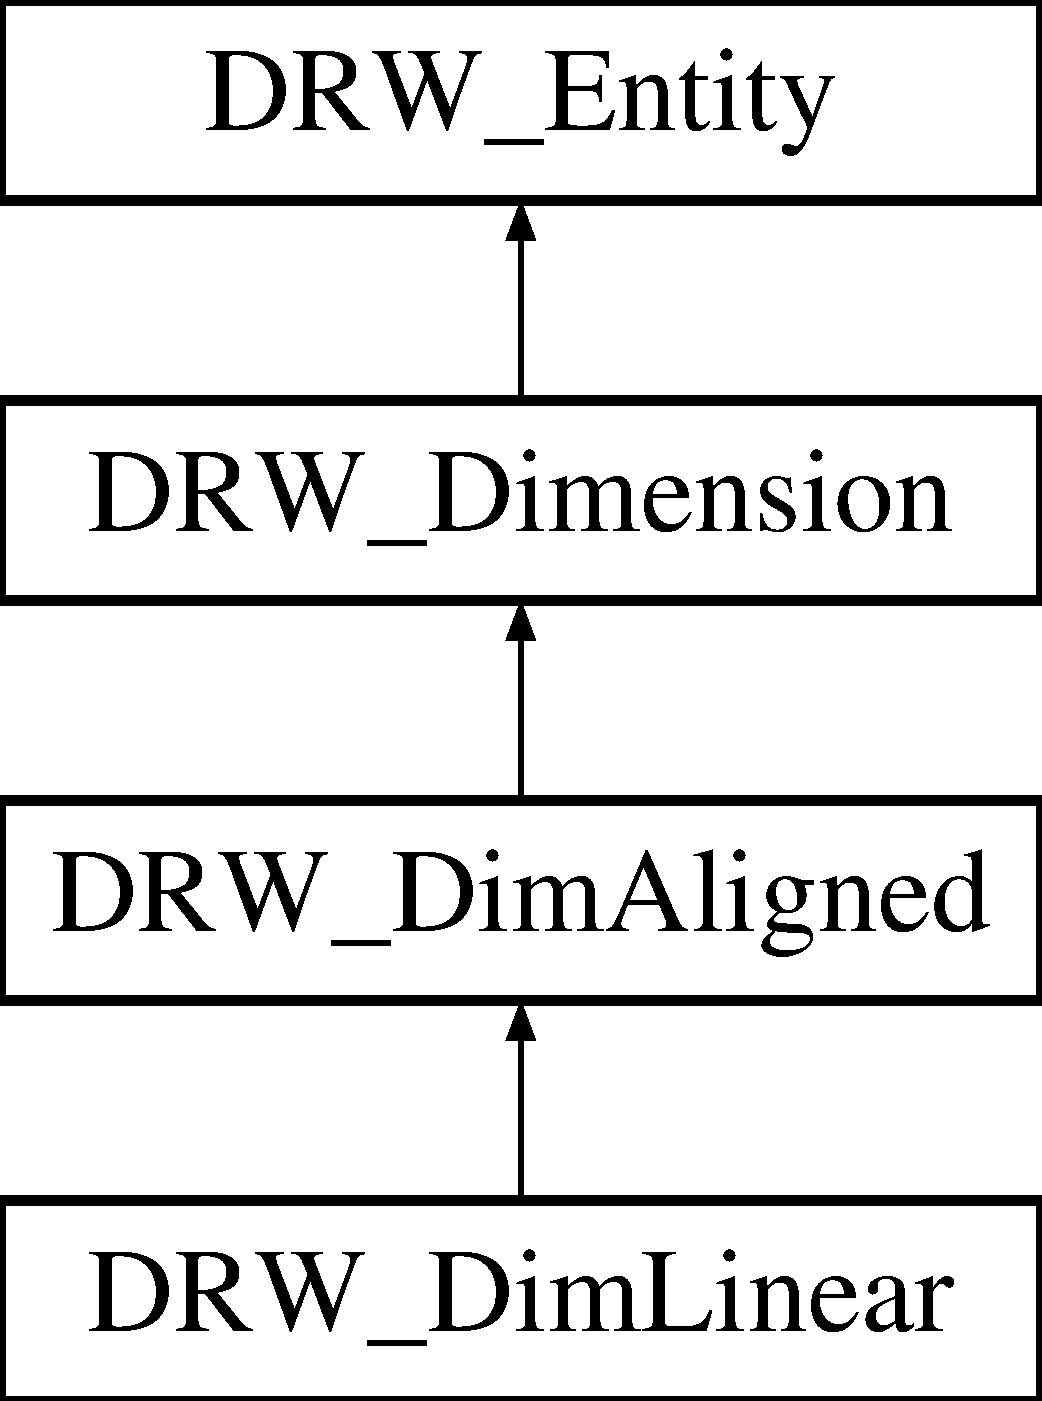
\includegraphics[height=4.000000cm]{db/df3/class_d_r_w___dim_linear}
\end{center}
\end{figure}
\subsection*{Public Member Functions}
\begin{DoxyCompactItemize}
\item 
double \hyperlink{class_d_r_w___dim_linear_ab383c82c37c4a4db5b91c2d56676cf89}{get\+Angle} () const 
\item 
double \hyperlink{class_d_r_w___dim_linear_a0ca1a1e9273e6ed0ac400a9352d6fb93}{get\+Oblique} () const 
\end{DoxyCompactItemize}
\subsection*{Additional Inherited Members}


\subsection{Detailed Description}
Class to handle linear or rotated dimension entity. 

Class to handle linear or rotated dimension entity \begin{DoxyAuthor}{Author}
Rallaz 
\end{DoxyAuthor}


\subsection{Member Function Documentation}
\hypertarget{class_d_r_w___dim_linear_ab383c82c37c4a4db5b91c2d56676cf89}{}\index{D\+R\+W\+\_\+\+Dim\+Linear@{D\+R\+W\+\_\+\+Dim\+Linear}!get\+Angle@{get\+Angle}}
\index{get\+Angle@{get\+Angle}!D\+R\+W\+\_\+\+Dim\+Linear@{D\+R\+W\+\_\+\+Dim\+Linear}}
\subsubsection[{get\+Angle}]{\setlength{\rightskip}{0pt plus 5cm}double D\+R\+W\+\_\+\+Dim\+Linear\+::get\+Angle (
\begin{DoxyParamCaption}
{}
\end{DoxyParamCaption}
) const\hspace{0.3cm}{\ttfamily [inline]}}\label{class_d_r_w___dim_linear_ab383c82c37c4a4db5b91c2d56676cf89}
Angle of rotated, horizontal, or vertical dimensions, code 50 \hypertarget{class_d_r_w___dim_linear_a0ca1a1e9273e6ed0ac400a9352d6fb93}{}\index{D\+R\+W\+\_\+\+Dim\+Linear@{D\+R\+W\+\_\+\+Dim\+Linear}!get\+Oblique@{get\+Oblique}}
\index{get\+Oblique@{get\+Oblique}!D\+R\+W\+\_\+\+Dim\+Linear@{D\+R\+W\+\_\+\+Dim\+Linear}}
\subsubsection[{get\+Oblique}]{\setlength{\rightskip}{0pt plus 5cm}double D\+R\+W\+\_\+\+Dim\+Linear\+::get\+Oblique (
\begin{DoxyParamCaption}
{}
\end{DoxyParamCaption}
) const\hspace{0.3cm}{\ttfamily [inline]}}\label{class_d_r_w___dim_linear_a0ca1a1e9273e6ed0ac400a9352d6fb93}
oblique angle, code 52 

The documentation for this class was generated from the following file\+:\begin{DoxyCompactItemize}
\item 
src/drw\+\_\+entities.\+h\end{DoxyCompactItemize}

\hypertarget{class_d_r_w___dim_ordinate}{}\section{D\+R\+W\+\_\+\+Dim\+Ordinate Class Reference}
\label{class_d_r_w___dim_ordinate}\index{D\+R\+W\+\_\+\+Dim\+Ordinate@{D\+R\+W\+\_\+\+Dim\+Ordinate}}


Class to handle ordinate dimension entity.  




{\ttfamily \#include $<$drw\+\_\+entities.\+h$>$}

Inheritance diagram for D\+R\+W\+\_\+\+Dim\+Ordinate\+:\begin{figure}[H]
\begin{center}
\leavevmode
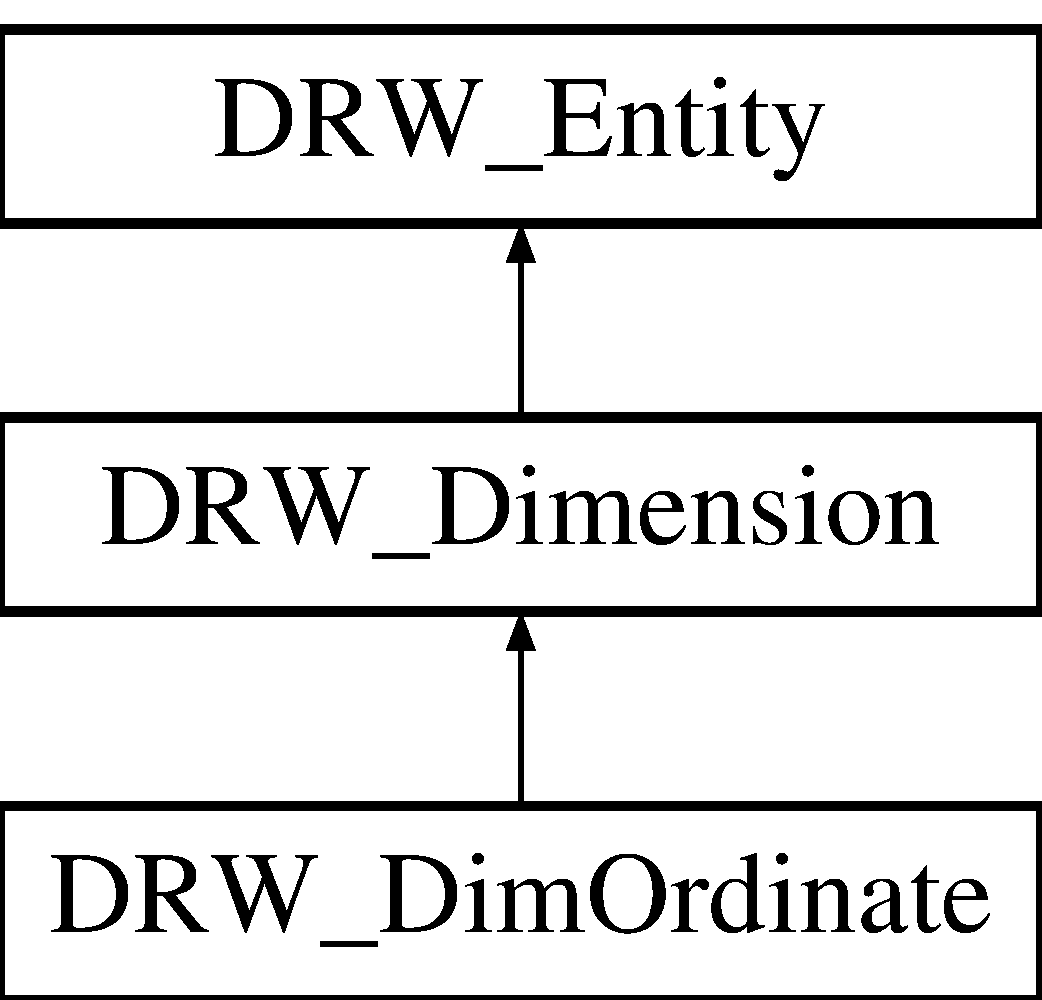
\includegraphics[height=3.000000cm]{d7/d1e/class_d_r_w___dim_ordinate}
\end{center}
\end{figure}
\subsection*{Public Member Functions}
\begin{DoxyCompactItemize}
\item 
\hyperlink{class_d_r_w___coord}{D\+R\+W\+\_\+\+Coord} \hyperlink{class_d_r_w___dim_ordinate_a8edf6d0926e228257425da4dc76b0b46}{get\+Origin\+Point} () const 
\item 
\hyperlink{class_d_r_w___coord}{D\+R\+W\+\_\+\+Coord} \hyperlink{class_d_r_w___dim_ordinate_a4effa3ec976e12b2cf7ade6caced2cfb}{get\+First\+Line} () const 
\item 
\hyperlink{class_d_r_w___coord}{D\+R\+W\+\_\+\+Coord} \hyperlink{class_d_r_w___dim_ordinate_afff3c4532e4d7bccf97867b96dc36491}{get\+Second\+Line} () const 
\end{DoxyCompactItemize}
\subsection*{Additional Inherited Members}


\subsection{Detailed Description}
Class to handle ordinate dimension entity. 

Class to handle ordinate dimension entity \begin{DoxyAuthor}{Author}
Rallaz 
\end{DoxyAuthor}


\subsection{Member Function Documentation}
\hypertarget{class_d_r_w___dim_ordinate_a4effa3ec976e12b2cf7ade6caced2cfb}{}\index{D\+R\+W\+\_\+\+Dim\+Ordinate@{D\+R\+W\+\_\+\+Dim\+Ordinate}!get\+First\+Line@{get\+First\+Line}}
\index{get\+First\+Line@{get\+First\+Line}!D\+R\+W\+\_\+\+Dim\+Ordinate@{D\+R\+W\+\_\+\+Dim\+Ordinate}}
\subsubsection[{get\+First\+Line}]{\setlength{\rightskip}{0pt plus 5cm}{\bf D\+R\+W\+\_\+\+Coord} D\+R\+W\+\_\+\+Dim\+Ordinate\+::get\+First\+Line (
\begin{DoxyParamCaption}
{}
\end{DoxyParamCaption}
) const\hspace{0.3cm}{\ttfamily [inline]}}\label{class_d_r_w___dim_ordinate_a4effa3ec976e12b2cf7ade6caced2cfb}
Feature location point, code 13, 23 \& 33 \hypertarget{class_d_r_w___dim_ordinate_a8edf6d0926e228257425da4dc76b0b46}{}\index{D\+R\+W\+\_\+\+Dim\+Ordinate@{D\+R\+W\+\_\+\+Dim\+Ordinate}!get\+Origin\+Point@{get\+Origin\+Point}}
\index{get\+Origin\+Point@{get\+Origin\+Point}!D\+R\+W\+\_\+\+Dim\+Ordinate@{D\+R\+W\+\_\+\+Dim\+Ordinate}}
\subsubsection[{get\+Origin\+Point}]{\setlength{\rightskip}{0pt plus 5cm}{\bf D\+R\+W\+\_\+\+Coord} D\+R\+W\+\_\+\+Dim\+Ordinate\+::get\+Origin\+Point (
\begin{DoxyParamCaption}
{}
\end{DoxyParamCaption}
) const\hspace{0.3cm}{\ttfamily [inline]}}\label{class_d_r_w___dim_ordinate_a8edf6d0926e228257425da4dc76b0b46}
Origin definition point, code 10, 20 \& 30 \hypertarget{class_d_r_w___dim_ordinate_afff3c4532e4d7bccf97867b96dc36491}{}\index{D\+R\+W\+\_\+\+Dim\+Ordinate@{D\+R\+W\+\_\+\+Dim\+Ordinate}!get\+Second\+Line@{get\+Second\+Line}}
\index{get\+Second\+Line@{get\+Second\+Line}!D\+R\+W\+\_\+\+Dim\+Ordinate@{D\+R\+W\+\_\+\+Dim\+Ordinate}}
\subsubsection[{get\+Second\+Line}]{\setlength{\rightskip}{0pt plus 5cm}{\bf D\+R\+W\+\_\+\+Coord} D\+R\+W\+\_\+\+Dim\+Ordinate\+::get\+Second\+Line (
\begin{DoxyParamCaption}
{}
\end{DoxyParamCaption}
) const\hspace{0.3cm}{\ttfamily [inline]}}\label{class_d_r_w___dim_ordinate_afff3c4532e4d7bccf97867b96dc36491}
Leader end point, code 14, 24 \& 34 

The documentation for this class was generated from the following file\+:\begin{DoxyCompactItemize}
\item 
src/drw\+\_\+entities.\+h\end{DoxyCompactItemize}

\hypertarget{class_d_r_w___dim_radial}{}\section{D\+R\+W\+\_\+\+Dim\+Radial Class Reference}
\label{class_d_r_w___dim_radial}\index{D\+R\+W\+\_\+\+Dim\+Radial@{D\+R\+W\+\_\+\+Dim\+Radial}}


Class to handle radial dimension entity.  




{\ttfamily \#include $<$drw\+\_\+entities.\+h$>$}

Inheritance diagram for D\+R\+W\+\_\+\+Dim\+Radial\+:\begin{figure}[H]
\begin{center}
\leavevmode
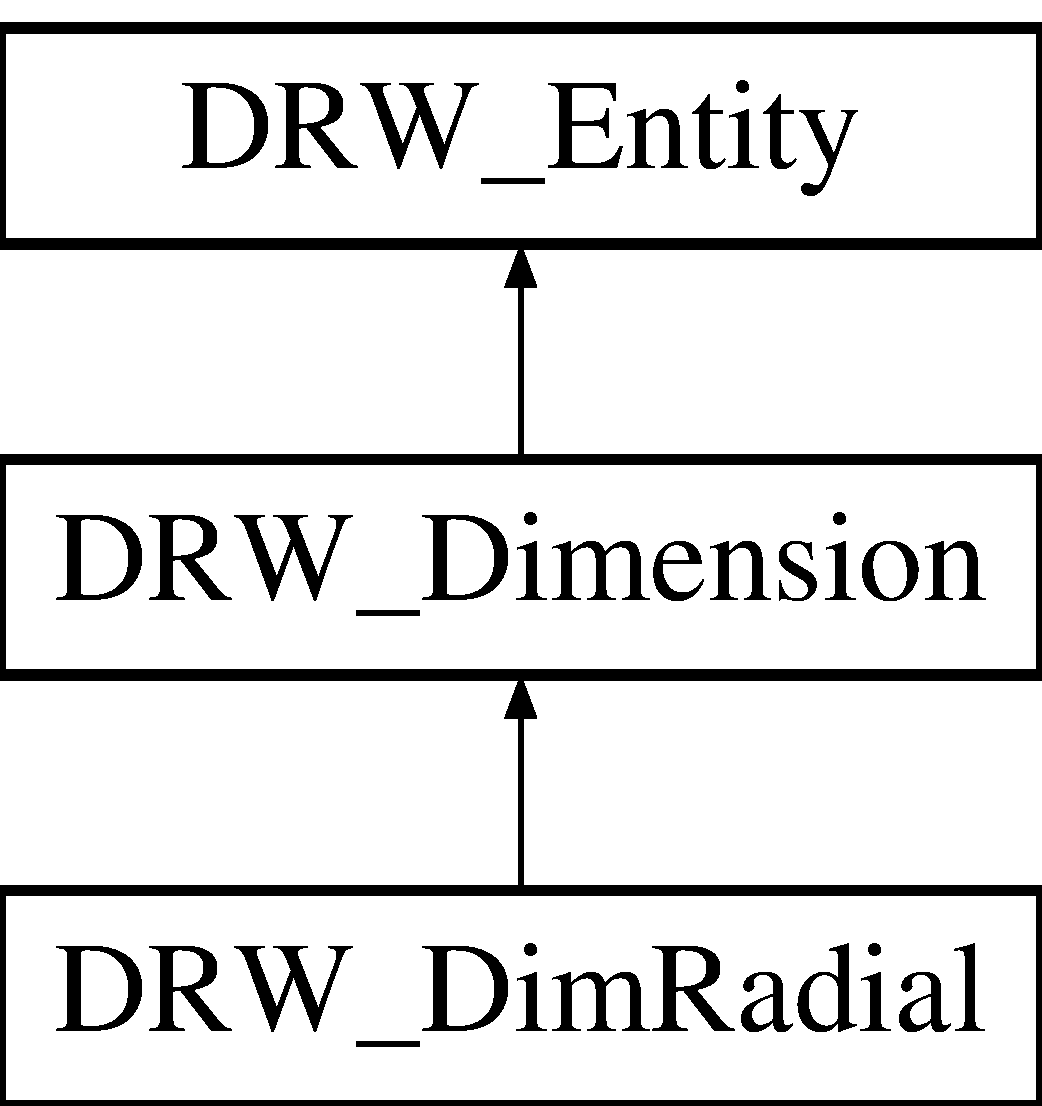
\includegraphics[height=3.000000cm]{da/d95/class_d_r_w___dim_radial}
\end{center}
\end{figure}
\subsection*{Public Member Functions}
\begin{DoxyCompactItemize}
\item 
\hyperlink{class_d_r_w___coord}{D\+R\+W\+\_\+\+Coord} \hyperlink{class_d_r_w___dim_radial_a81bb02a4fd5574ac4bd2321ed7936b22}{get\+Center\+Point} () const 
\item 
\hyperlink{class_d_r_w___coord}{D\+R\+W\+\_\+\+Coord} \hyperlink{class_d_r_w___dim_radial_ac0c68b23a408f7f9c12a8b1d6ef6f4db}{get\+Diameter\+Point} () const 
\item 
double \hyperlink{class_d_r_w___dim_radial_ab1127a65b14758a780d3e2e4a3b0b102}{get\+Leader\+Length} () const 
\end{DoxyCompactItemize}
\subsection*{Additional Inherited Members}


\subsection{Detailed Description}
Class to handle radial dimension entity. 

Class to handle aligned, linear or rotated dimension entity \begin{DoxyAuthor}{Author}
Rallaz 
\end{DoxyAuthor}


\subsection{Member Function Documentation}
\hypertarget{class_d_r_w___dim_radial_a81bb02a4fd5574ac4bd2321ed7936b22}{}\index{D\+R\+W\+\_\+\+Dim\+Radial@{D\+R\+W\+\_\+\+Dim\+Radial}!get\+Center\+Point@{get\+Center\+Point}}
\index{get\+Center\+Point@{get\+Center\+Point}!D\+R\+W\+\_\+\+Dim\+Radial@{D\+R\+W\+\_\+\+Dim\+Radial}}
\subsubsection[{get\+Center\+Point}]{\setlength{\rightskip}{0pt plus 5cm}{\bf D\+R\+W\+\_\+\+Coord} D\+R\+W\+\_\+\+Dim\+Radial\+::get\+Center\+Point (
\begin{DoxyParamCaption}
{}
\end{DoxyParamCaption}
) const\hspace{0.3cm}{\ttfamily [inline]}}\label{class_d_r_w___dim_radial_a81bb02a4fd5574ac4bd2321ed7936b22}
center point, code 10, 20 \& 30 \hypertarget{class_d_r_w___dim_radial_ac0c68b23a408f7f9c12a8b1d6ef6f4db}{}\index{D\+R\+W\+\_\+\+Dim\+Radial@{D\+R\+W\+\_\+\+Dim\+Radial}!get\+Diameter\+Point@{get\+Diameter\+Point}}
\index{get\+Diameter\+Point@{get\+Diameter\+Point}!D\+R\+W\+\_\+\+Dim\+Radial@{D\+R\+W\+\_\+\+Dim\+Radial}}
\subsubsection[{get\+Diameter\+Point}]{\setlength{\rightskip}{0pt plus 5cm}{\bf D\+R\+W\+\_\+\+Coord} D\+R\+W\+\_\+\+Dim\+Radial\+::get\+Diameter\+Point (
\begin{DoxyParamCaption}
{}
\end{DoxyParamCaption}
) const\hspace{0.3cm}{\ttfamily [inline]}}\label{class_d_r_w___dim_radial_ac0c68b23a408f7f9c12a8b1d6ef6f4db}
Definition point for radius, code 15, 25 \& 35 \hypertarget{class_d_r_w___dim_radial_ab1127a65b14758a780d3e2e4a3b0b102}{}\index{D\+R\+W\+\_\+\+Dim\+Radial@{D\+R\+W\+\_\+\+Dim\+Radial}!get\+Leader\+Length@{get\+Leader\+Length}}
\index{get\+Leader\+Length@{get\+Leader\+Length}!D\+R\+W\+\_\+\+Dim\+Radial@{D\+R\+W\+\_\+\+Dim\+Radial}}
\subsubsection[{get\+Leader\+Length}]{\setlength{\rightskip}{0pt plus 5cm}double D\+R\+W\+\_\+\+Dim\+Radial\+::get\+Leader\+Length (
\begin{DoxyParamCaption}
{}
\end{DoxyParamCaption}
) const\hspace{0.3cm}{\ttfamily [inline]}}\label{class_d_r_w___dim_radial_ab1127a65b14758a780d3e2e4a3b0b102}
Leader length, code 40 

The documentation for this class was generated from the following file\+:\begin{DoxyCompactItemize}
\item 
src/drw\+\_\+entities.\+h\end{DoxyCompactItemize}

\hypertarget{class_d_r_w___dimstyle}{}\section{D\+R\+W\+\_\+\+Dimstyle Class Reference}
\label{class_d_r_w___dimstyle}\index{D\+R\+W\+\_\+\+Dimstyle@{D\+R\+W\+\_\+\+Dimstyle}}


Class to handle dimstyle entries.  




{\ttfamily \#include $<$drw\+\_\+objects.\+h$>$}

Inheritance diagram for D\+R\+W\+\_\+\+Dimstyle\+:\begin{figure}[H]
\begin{center}
\leavevmode
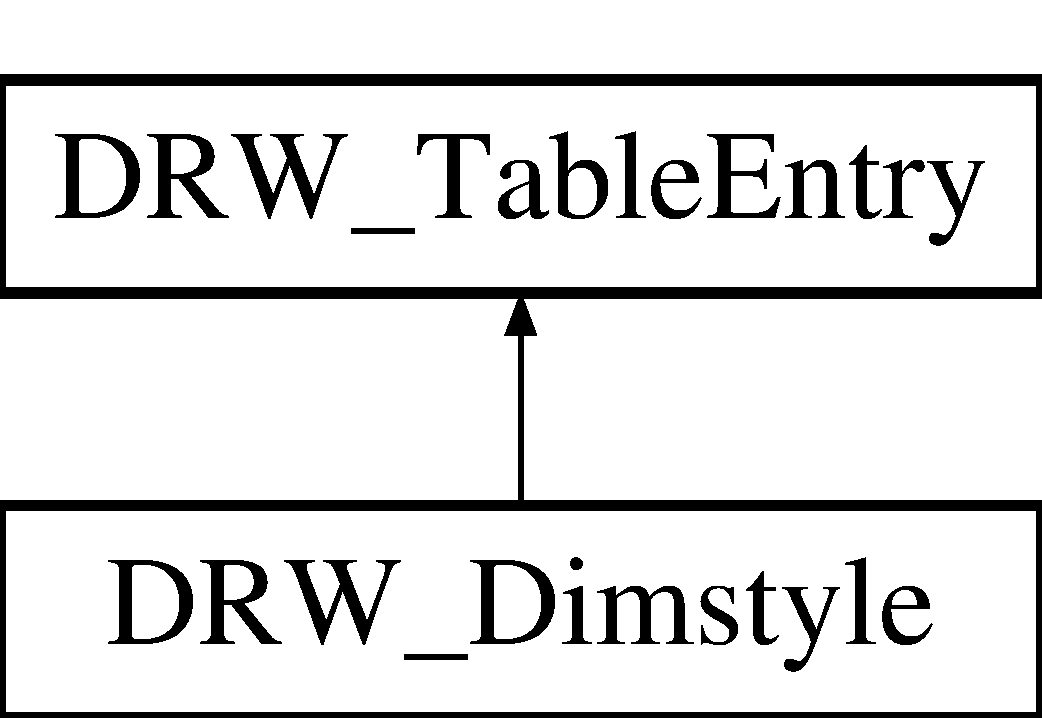
\includegraphics[height=2.000000cm]{dc/dad/class_d_r_w___dimstyle}
\end{center}
\end{figure}
\subsection*{Public Member Functions}
\begin{DoxyCompactItemize}
\item 
void \hyperlink{class_d_r_w___dimstyle_a31a3e3bf8780ee8b7b08efc145125e96}{parse\+Code} (int code, dxf\+Reader $\ast$reader)
\begin{DoxyCompactList}\small\item\em Class to handle dimstyle entries. \end{DoxyCompactList}\end{DoxyCompactItemize}
\subsection*{Public Attributes}
\begin{DoxyCompactItemize}
\item 
U\+T\+F8\+S\+T\+R\+I\+N\+G \hyperlink{class_d_r_w___dimstyle_ab4484303cfced1d7ad3c19a84b19dada}{dimpost}
\item 
U\+T\+F8\+S\+T\+R\+I\+N\+G \hyperlink{class_d_r_w___dimstyle_a933deca82de6d15d82ada90f8731a00b}{dimapost}
\item 
U\+T\+F8\+S\+T\+R\+I\+N\+G \hyperlink{class_d_r_w___dimstyle_a2f64034b5654fee47038933c565a2e51}{dimblk}
\item 
U\+T\+F8\+S\+T\+R\+I\+N\+G \hyperlink{class_d_r_w___dimstyle_a33a57c5c614537649e042eef57a03f9d}{dimblk1}
\item 
U\+T\+F8\+S\+T\+R\+I\+N\+G \hyperlink{class_d_r_w___dimstyle_a65761962dbaff5d150f4a9296efeadfc}{dimblk2}
\item 
double \hyperlink{class_d_r_w___dimstyle_a2b9d92349258970f08efd3bd25d8cfd2}{dimscale}
\item 
double \hyperlink{class_d_r_w___dimstyle_ae0ea0ac39cd2e961ccf4c3b54c570967}{dimasz}
\item 
double \hyperlink{class_d_r_w___dimstyle_a22b63c5e53a889bfd549cc476e5bdd4a}{dimexo}
\item 
double \hyperlink{class_d_r_w___dimstyle_a6d13f43f1689621623c4193501ddb5cc}{dimdli}
\item 
double \hyperlink{class_d_r_w___dimstyle_af1d89fe302b0147db6db850a6382b743}{dimexe}
\item 
double \hyperlink{class_d_r_w___dimstyle_abe4aea95c5bf8eca979c33d94ea2bb07}{dimrnd}
\item 
double \hyperlink{class_d_r_w___dimstyle_a7aebc776b75660bc9947a90416bf8ab4}{dimdle}
\item 
double \hyperlink{class_d_r_w___dimstyle_a6596806a922534a220ce3b7f7b4bb415}{dimtp}
\item 
double \hyperlink{class_d_r_w___dimstyle_a80ccee76ee51137e11097fc61bc81329}{dimtm}
\item 
double \hyperlink{class_d_r_w___dimstyle_a8cc804b4094615949f6b314375d2e726}{dimtxt}
\item 
double \hyperlink{class_d_r_w___dimstyle_a3b2ea8efe76c60db85c14dcc8724a7f6}{dimcen}
\item 
double \hyperlink{class_d_r_w___dimstyle_a4b8018caf9bdf34b2002efce8929dc57}{dimtsz}
\item 
double \hyperlink{class_d_r_w___dimstyle_a0ccbe896838b874d8bdf263b48e7cee6}{dimaltf}
\item 
double \hyperlink{class_d_r_w___dimstyle_ac74c4cc07bf6edde4b563d8f5fb03d8e}{dimlfac}
\item 
double \hyperlink{class_d_r_w___dimstyle_a002065c5911ff94712dd7d688b886883}{dimtvp}
\item 
double \hyperlink{class_d_r_w___dimstyle_af90d8887451dfd6c127d27baa014735a}{dimtfac}
\item 
double \hyperlink{class_d_r_w___dimstyle_af258a983498f66472b6c5b51d368980b}{dimgap}
\item 
double \hyperlink{class_d_r_w___dimstyle_a023f32391a544dc81aabadd2e163f90d}{dimaltrnd}
\item 
int \hyperlink{class_d_r_w___dimstyle_a68bc1acdadaa4511180645a648c911a1}{dimtol}
\item 
int \hyperlink{class_d_r_w___dimstyle_ae5324505be40acd3ed0450d39d3bd120}{dimlim}
\item 
int \hyperlink{class_d_r_w___dimstyle_add00c697c40fbc99d7f33af58ac3a75b}{dimtih}
\item 
int \hyperlink{class_d_r_w___dimstyle_a1b18fcdd37b17dda1613d19b3302c7b1}{dimtoh}
\item 
int \hyperlink{class_d_r_w___dimstyle_ab22248ba9479af5636e522d9bbaf098d}{dimse1}
\item 
int \hyperlink{class_d_r_w___dimstyle_a216852cf21ff08714ec7ce33085a7d76}{dimse2}
\item 
int \hyperlink{class_d_r_w___dimstyle_a5d98411bf63dd31343050ee3b17778ef}{dimtad}
\item 
int \hyperlink{class_d_r_w___dimstyle_a4922b8e483f9e2ae67ea92aa4f7503c8}{dimzin}
\item 
int \hyperlink{class_d_r_w___dimstyle_a5e3f7207c9924cd3f14b440f1db86f96}{dimazin}
\item 
int \hyperlink{class_d_r_w___dimstyle_a1e1e9ec596e0d157c75fffd91bd20df2}{dimalt}
\item 
int \hyperlink{class_d_r_w___dimstyle_aefeeeccbe986c9484b59024c8bc40a98}{dimaltd}
\item 
int \hyperlink{class_d_r_w___dimstyle_a23a67180f9fb818301a9a9596818eabb}{dimtofl}
\item 
int \hyperlink{class_d_r_w___dimstyle_aa0bbdb436f7fe738ee5566a2a447170d}{dimsah}
\item 
int \hyperlink{class_d_r_w___dimstyle_a382ba0d93da78f97e93c97ef87edfc62}{dimtix}
\item 
int \hyperlink{class_d_r_w___dimstyle_aeb06ebd1bd16306b336032f4b8c4a80a}{dimsoxd}
\item 
int \hyperlink{class_d_r_w___dimstyle_ae1768dfc1e5a2986125affd928cc1278}{dimclrd}
\item 
int \hyperlink{class_d_r_w___dimstyle_ad603cb462dc00136ff50933979b0aab7}{dimclre}
\item 
int \hyperlink{class_d_r_w___dimstyle_ae89e4a003314815b40b00c26b0cb0ba0}{dimclrt}
\item 
int \hyperlink{class_d_r_w___dimstyle_a3954f6b5e068cb1fd157231af5680e81}{dimadec}
\item 
int \hyperlink{class_d_r_w___dimstyle_a6772e7086bdfff0c3c73892eb9068f90}{dimunit}
\item 
int \hyperlink{class_d_r_w___dimstyle_af71e0007f9eaddb929e7c405fdb365bb}{dimdec}
\item 
int \hyperlink{class_d_r_w___dimstyle_adf05a8cee69d5a24cff03bccb74fdaf0}{dimtdec}
\item 
int \hyperlink{class_d_r_w___dimstyle_afa6555bf1abbabe03f6a48a9b8e1026c}{dimaltu}
\item 
int \hyperlink{class_d_r_w___dimstyle_a3856be49d2e138cc1c6605ae1bf7b14a}{dimalttd}
\item 
int \hyperlink{class_d_r_w___dimstyle_a2f0ddeaf2ca3e3dc5a4e35c7fb509939}{dimaunit}
\item 
int \hyperlink{class_d_r_w___dimstyle_aa1c69e4b8d22cc906db95161d110d115}{dimfrac}
\item 
int \hyperlink{class_d_r_w___dimstyle_a3e2bc803306737f75c7a0390c0dbc5cd}{dimlunit}
\item 
int \hyperlink{class_d_r_w___dimstyle_a55bca8cbe1928c4f9cbde1c07041c121}{dimdsep}
\item 
int \hyperlink{class_d_r_w___dimstyle_a6dfa91db09ae5fa28ea09cb752251a74}{dimtmove}
\item 
int \hyperlink{class_d_r_w___dimstyle_a065205dcc5446262657b612353aa3deb}{dimjust}
\item 
int \hyperlink{class_d_r_w___dimstyle_a67e56dca697de6cb0514ba2e95a0907f}{dimsd1}
\item 
int \hyperlink{class_d_r_w___dimstyle_adee8bad44d6c486361c2809c0eeca8d6}{dimsd2}
\item 
int \hyperlink{class_d_r_w___dimstyle_a0aff1bb2b68293702729f84e751bea0a}{dimtolj}
\item 
int \hyperlink{class_d_r_w___dimstyle_a1c84c1ead844589af50adf72ab59d7dc}{dimtzin}
\item 
int \hyperlink{class_d_r_w___dimstyle_a841079cef255e9f6d06d7b97a28c67ec}{dimaltz}
\item 
int \hyperlink{class_d_r_w___dimstyle_af4c0b630cd4485a16cafe42ddcda6b0a}{dimaltttz}
\item 
int \hyperlink{class_d_r_w___dimstyle_a6ea2dea32359478e0b37777f679d212c}{dimfit}
\item 
int \hyperlink{class_d_r_w___dimstyle_ada5b945b12f79ebe3246b9b4830eab68}{dimupt}
\item 
int \hyperlink{class_d_r_w___dimstyle_a573b46a58131b108589f35bb67c9800f}{dimatfit}
\item 
U\+T\+F8\+S\+T\+R\+I\+N\+G \hyperlink{class_d_r_w___dimstyle_a864803fca4c604cf16d073a8a5bed0c2}{dimtxsty}
\item 
U\+T\+F8\+S\+T\+R\+I\+N\+G \hyperlink{class_d_r_w___dimstyle_a975377a787e4ca8a515f20f277d7a805}{dimldrblk}
\item 
int \hyperlink{class_d_r_w___dimstyle_a1547ae00544ee4cc865e30847220b5a3}{dimlwd}
\item 
int \hyperlink{class_d_r_w___dimstyle_a25f9fed17c3cbd6f0969d85a0fc42df4}{dimlwe}
\end{DoxyCompactItemize}
\subsection*{Additional Inherited Members}


\subsection{Detailed Description}
Class to handle dimstyle entries. 

Class to handle dim style symbol table entries \begin{DoxyAuthor}{Author}
Rallaz 
\end{DoxyAuthor}


\subsection{Member Function Documentation}
\hypertarget{class_d_r_w___dimstyle_a31a3e3bf8780ee8b7b08efc145125e96}{}\index{D\+R\+W\+\_\+\+Dimstyle@{D\+R\+W\+\_\+\+Dimstyle}!parse\+Code@{parse\+Code}}
\index{parse\+Code@{parse\+Code}!D\+R\+W\+\_\+\+Dimstyle@{D\+R\+W\+\_\+\+Dimstyle}}
\subsubsection[{parse\+Code}]{\setlength{\rightskip}{0pt plus 5cm}void D\+R\+W\+\_\+\+Dimstyle\+::parse\+Code (
\begin{DoxyParamCaption}
\item[{int}]{code, }
\item[{dxf\+Reader $\ast$}]{reader}
\end{DoxyParamCaption}
)}\label{class_d_r_w___dimstyle_a31a3e3bf8780ee8b7b08efc145125e96}


Class to handle dimstyle entries. 

Class to handle ldim style symbol table entries \begin{DoxyAuthor}{Author}
Rallaz 
\end{DoxyAuthor}


\subsection{Member Data Documentation}
\hypertarget{class_d_r_w___dimstyle_a3954f6b5e068cb1fd157231af5680e81}{}\index{D\+R\+W\+\_\+\+Dimstyle@{D\+R\+W\+\_\+\+Dimstyle}!dimadec@{dimadec}}
\index{dimadec@{dimadec}!D\+R\+W\+\_\+\+Dimstyle@{D\+R\+W\+\_\+\+Dimstyle}}
\subsubsection[{dimadec}]{\setlength{\rightskip}{0pt plus 5cm}int D\+R\+W\+\_\+\+Dimstyle\+::dimadec}\label{class_d_r_w___dimstyle_a3954f6b5e068cb1fd157231af5680e81}
code 179 V2000+ \hypertarget{class_d_r_w___dimstyle_a1e1e9ec596e0d157c75fffd91bd20df2}{}\index{D\+R\+W\+\_\+\+Dimstyle@{D\+R\+W\+\_\+\+Dimstyle}!dimalt@{dimalt}}
\index{dimalt@{dimalt}!D\+R\+W\+\_\+\+Dimstyle@{D\+R\+W\+\_\+\+Dimstyle}}
\subsubsection[{dimalt}]{\setlength{\rightskip}{0pt plus 5cm}int D\+R\+W\+\_\+\+Dimstyle\+::dimalt}\label{class_d_r_w___dimstyle_a1e1e9ec596e0d157c75fffd91bd20df2}
code 170 \hypertarget{class_d_r_w___dimstyle_aefeeeccbe986c9484b59024c8bc40a98}{}\index{D\+R\+W\+\_\+\+Dimstyle@{D\+R\+W\+\_\+\+Dimstyle}!dimaltd@{dimaltd}}
\index{dimaltd@{dimaltd}!D\+R\+W\+\_\+\+Dimstyle@{D\+R\+W\+\_\+\+Dimstyle}}
\subsubsection[{dimaltd}]{\setlength{\rightskip}{0pt plus 5cm}int D\+R\+W\+\_\+\+Dimstyle\+::dimaltd}\label{class_d_r_w___dimstyle_aefeeeccbe986c9484b59024c8bc40a98}
code 171 \hypertarget{class_d_r_w___dimstyle_a0ccbe896838b874d8bdf263b48e7cee6}{}\index{D\+R\+W\+\_\+\+Dimstyle@{D\+R\+W\+\_\+\+Dimstyle}!dimaltf@{dimaltf}}
\index{dimaltf@{dimaltf}!D\+R\+W\+\_\+\+Dimstyle@{D\+R\+W\+\_\+\+Dimstyle}}
\subsubsection[{dimaltf}]{\setlength{\rightskip}{0pt plus 5cm}double D\+R\+W\+\_\+\+Dimstyle\+::dimaltf}\label{class_d_r_w___dimstyle_a0ccbe896838b874d8bdf263b48e7cee6}
code 143 \hypertarget{class_d_r_w___dimstyle_a023f32391a544dc81aabadd2e163f90d}{}\index{D\+R\+W\+\_\+\+Dimstyle@{D\+R\+W\+\_\+\+Dimstyle}!dimaltrnd@{dimaltrnd}}
\index{dimaltrnd@{dimaltrnd}!D\+R\+W\+\_\+\+Dimstyle@{D\+R\+W\+\_\+\+Dimstyle}}
\subsubsection[{dimaltrnd}]{\setlength{\rightskip}{0pt plus 5cm}double D\+R\+W\+\_\+\+Dimstyle\+::dimaltrnd}\label{class_d_r_w___dimstyle_a023f32391a544dc81aabadd2e163f90d}
code 148 V2000+ \hypertarget{class_d_r_w___dimstyle_a3856be49d2e138cc1c6605ae1bf7b14a}{}\index{D\+R\+W\+\_\+\+Dimstyle@{D\+R\+W\+\_\+\+Dimstyle}!dimalttd@{dimalttd}}
\index{dimalttd@{dimalttd}!D\+R\+W\+\_\+\+Dimstyle@{D\+R\+W\+\_\+\+Dimstyle}}
\subsubsection[{dimalttd}]{\setlength{\rightskip}{0pt plus 5cm}int D\+R\+W\+\_\+\+Dimstyle\+::dimalttd}\label{class_d_r_w___dimstyle_a3856be49d2e138cc1c6605ae1bf7b14a}
code 274 R13+ \hypertarget{class_d_r_w___dimstyle_af4c0b630cd4485a16cafe42ddcda6b0a}{}\index{D\+R\+W\+\_\+\+Dimstyle@{D\+R\+W\+\_\+\+Dimstyle}!dimaltttz@{dimaltttz}}
\index{dimaltttz@{dimaltttz}!D\+R\+W\+\_\+\+Dimstyle@{D\+R\+W\+\_\+\+Dimstyle}}
\subsubsection[{dimaltttz}]{\setlength{\rightskip}{0pt plus 5cm}int D\+R\+W\+\_\+\+Dimstyle\+::dimaltttz}\label{class_d_r_w___dimstyle_af4c0b630cd4485a16cafe42ddcda6b0a}
code 286 R13+ \hypertarget{class_d_r_w___dimstyle_afa6555bf1abbabe03f6a48a9b8e1026c}{}\index{D\+R\+W\+\_\+\+Dimstyle@{D\+R\+W\+\_\+\+Dimstyle}!dimaltu@{dimaltu}}
\index{dimaltu@{dimaltu}!D\+R\+W\+\_\+\+Dimstyle@{D\+R\+W\+\_\+\+Dimstyle}}
\subsubsection[{dimaltu}]{\setlength{\rightskip}{0pt plus 5cm}int D\+R\+W\+\_\+\+Dimstyle\+::dimaltu}\label{class_d_r_w___dimstyle_afa6555bf1abbabe03f6a48a9b8e1026c}
code 273 R13+ \hypertarget{class_d_r_w___dimstyle_a841079cef255e9f6d06d7b97a28c67ec}{}\index{D\+R\+W\+\_\+\+Dimstyle@{D\+R\+W\+\_\+\+Dimstyle}!dimaltz@{dimaltz}}
\index{dimaltz@{dimaltz}!D\+R\+W\+\_\+\+Dimstyle@{D\+R\+W\+\_\+\+Dimstyle}}
\subsubsection[{dimaltz}]{\setlength{\rightskip}{0pt plus 5cm}int D\+R\+W\+\_\+\+Dimstyle\+::dimaltz}\label{class_d_r_w___dimstyle_a841079cef255e9f6d06d7b97a28c67ec}
code 285 R13+ \hypertarget{class_d_r_w___dimstyle_a933deca82de6d15d82ada90f8731a00b}{}\index{D\+R\+W\+\_\+\+Dimstyle@{D\+R\+W\+\_\+\+Dimstyle}!dimapost@{dimapost}}
\index{dimapost@{dimapost}!D\+R\+W\+\_\+\+Dimstyle@{D\+R\+W\+\_\+\+Dimstyle}}
\subsubsection[{dimapost}]{\setlength{\rightskip}{0pt plus 5cm}U\+T\+F8\+S\+T\+R\+I\+N\+G D\+R\+W\+\_\+\+Dimstyle\+::dimapost}\label{class_d_r_w___dimstyle_a933deca82de6d15d82ada90f8731a00b}
code 4 \hypertarget{class_d_r_w___dimstyle_ae0ea0ac39cd2e961ccf4c3b54c570967}{}\index{D\+R\+W\+\_\+\+Dimstyle@{D\+R\+W\+\_\+\+Dimstyle}!dimasz@{dimasz}}
\index{dimasz@{dimasz}!D\+R\+W\+\_\+\+Dimstyle@{D\+R\+W\+\_\+\+Dimstyle}}
\subsubsection[{dimasz}]{\setlength{\rightskip}{0pt plus 5cm}double D\+R\+W\+\_\+\+Dimstyle\+::dimasz}\label{class_d_r_w___dimstyle_ae0ea0ac39cd2e961ccf4c3b54c570967}
code 41 \hypertarget{class_d_r_w___dimstyle_a573b46a58131b108589f35bb67c9800f}{}\index{D\+R\+W\+\_\+\+Dimstyle@{D\+R\+W\+\_\+\+Dimstyle}!dimatfit@{dimatfit}}
\index{dimatfit@{dimatfit}!D\+R\+W\+\_\+\+Dimstyle@{D\+R\+W\+\_\+\+Dimstyle}}
\subsubsection[{dimatfit}]{\setlength{\rightskip}{0pt plus 5cm}int D\+R\+W\+\_\+\+Dimstyle\+::dimatfit}\label{class_d_r_w___dimstyle_a573b46a58131b108589f35bb67c9800f}
code 289 V2000+ \hypertarget{class_d_r_w___dimstyle_a2f0ddeaf2ca3e3dc5a4e35c7fb509939}{}\index{D\+R\+W\+\_\+\+Dimstyle@{D\+R\+W\+\_\+\+Dimstyle}!dimaunit@{dimaunit}}
\index{dimaunit@{dimaunit}!D\+R\+W\+\_\+\+Dimstyle@{D\+R\+W\+\_\+\+Dimstyle}}
\subsubsection[{dimaunit}]{\setlength{\rightskip}{0pt plus 5cm}int D\+R\+W\+\_\+\+Dimstyle\+::dimaunit}\label{class_d_r_w___dimstyle_a2f0ddeaf2ca3e3dc5a4e35c7fb509939}
code 275 R13+ \hypertarget{class_d_r_w___dimstyle_a5e3f7207c9924cd3f14b440f1db86f96}{}\index{D\+R\+W\+\_\+\+Dimstyle@{D\+R\+W\+\_\+\+Dimstyle}!dimazin@{dimazin}}
\index{dimazin@{dimazin}!D\+R\+W\+\_\+\+Dimstyle@{D\+R\+W\+\_\+\+Dimstyle}}
\subsubsection[{dimazin}]{\setlength{\rightskip}{0pt plus 5cm}int D\+R\+W\+\_\+\+Dimstyle\+::dimazin}\label{class_d_r_w___dimstyle_a5e3f7207c9924cd3f14b440f1db86f96}
code 79 V2000+ \hypertarget{class_d_r_w___dimstyle_a2f64034b5654fee47038933c565a2e51}{}\index{D\+R\+W\+\_\+\+Dimstyle@{D\+R\+W\+\_\+\+Dimstyle}!dimblk@{dimblk}}
\index{dimblk@{dimblk}!D\+R\+W\+\_\+\+Dimstyle@{D\+R\+W\+\_\+\+Dimstyle}}
\subsubsection[{dimblk}]{\setlength{\rightskip}{0pt plus 5cm}U\+T\+F8\+S\+T\+R\+I\+N\+G D\+R\+W\+\_\+\+Dimstyle\+::dimblk}\label{class_d_r_w___dimstyle_a2f64034b5654fee47038933c565a2e51}
code 5, code 342 V2000+ \hypertarget{class_d_r_w___dimstyle_a33a57c5c614537649e042eef57a03f9d}{}\index{D\+R\+W\+\_\+\+Dimstyle@{D\+R\+W\+\_\+\+Dimstyle}!dimblk1@{dimblk1}}
\index{dimblk1@{dimblk1}!D\+R\+W\+\_\+\+Dimstyle@{D\+R\+W\+\_\+\+Dimstyle}}
\subsubsection[{dimblk1}]{\setlength{\rightskip}{0pt plus 5cm}U\+T\+F8\+S\+T\+R\+I\+N\+G D\+R\+W\+\_\+\+Dimstyle\+::dimblk1}\label{class_d_r_w___dimstyle_a33a57c5c614537649e042eef57a03f9d}
code 6, code 343 V2000+ \hypertarget{class_d_r_w___dimstyle_a65761962dbaff5d150f4a9296efeadfc}{}\index{D\+R\+W\+\_\+\+Dimstyle@{D\+R\+W\+\_\+\+Dimstyle}!dimblk2@{dimblk2}}
\index{dimblk2@{dimblk2}!D\+R\+W\+\_\+\+Dimstyle@{D\+R\+W\+\_\+\+Dimstyle}}
\subsubsection[{dimblk2}]{\setlength{\rightskip}{0pt plus 5cm}U\+T\+F8\+S\+T\+R\+I\+N\+G D\+R\+W\+\_\+\+Dimstyle\+::dimblk2}\label{class_d_r_w___dimstyle_a65761962dbaff5d150f4a9296efeadfc}
code 7, code 344 V2000+ \hypertarget{class_d_r_w___dimstyle_a3b2ea8efe76c60db85c14dcc8724a7f6}{}\index{D\+R\+W\+\_\+\+Dimstyle@{D\+R\+W\+\_\+\+Dimstyle}!dimcen@{dimcen}}
\index{dimcen@{dimcen}!D\+R\+W\+\_\+\+Dimstyle@{D\+R\+W\+\_\+\+Dimstyle}}
\subsubsection[{dimcen}]{\setlength{\rightskip}{0pt plus 5cm}double D\+R\+W\+\_\+\+Dimstyle\+::dimcen}\label{class_d_r_w___dimstyle_a3b2ea8efe76c60db85c14dcc8724a7f6}
code 141 \hypertarget{class_d_r_w___dimstyle_ae1768dfc1e5a2986125affd928cc1278}{}\index{D\+R\+W\+\_\+\+Dimstyle@{D\+R\+W\+\_\+\+Dimstyle}!dimclrd@{dimclrd}}
\index{dimclrd@{dimclrd}!D\+R\+W\+\_\+\+Dimstyle@{D\+R\+W\+\_\+\+Dimstyle}}
\subsubsection[{dimclrd}]{\setlength{\rightskip}{0pt plus 5cm}int D\+R\+W\+\_\+\+Dimstyle\+::dimclrd}\label{class_d_r_w___dimstyle_ae1768dfc1e5a2986125affd928cc1278}
code 176 \hypertarget{class_d_r_w___dimstyle_ad603cb462dc00136ff50933979b0aab7}{}\index{D\+R\+W\+\_\+\+Dimstyle@{D\+R\+W\+\_\+\+Dimstyle}!dimclre@{dimclre}}
\index{dimclre@{dimclre}!D\+R\+W\+\_\+\+Dimstyle@{D\+R\+W\+\_\+\+Dimstyle}}
\subsubsection[{dimclre}]{\setlength{\rightskip}{0pt plus 5cm}int D\+R\+W\+\_\+\+Dimstyle\+::dimclre}\label{class_d_r_w___dimstyle_ad603cb462dc00136ff50933979b0aab7}
code 177 \hypertarget{class_d_r_w___dimstyle_ae89e4a003314815b40b00c26b0cb0ba0}{}\index{D\+R\+W\+\_\+\+Dimstyle@{D\+R\+W\+\_\+\+Dimstyle}!dimclrt@{dimclrt}}
\index{dimclrt@{dimclrt}!D\+R\+W\+\_\+\+Dimstyle@{D\+R\+W\+\_\+\+Dimstyle}}
\subsubsection[{dimclrt}]{\setlength{\rightskip}{0pt plus 5cm}int D\+R\+W\+\_\+\+Dimstyle\+::dimclrt}\label{class_d_r_w___dimstyle_ae89e4a003314815b40b00c26b0cb0ba0}
code 178 \hypertarget{class_d_r_w___dimstyle_af71e0007f9eaddb929e7c405fdb365bb}{}\index{D\+R\+W\+\_\+\+Dimstyle@{D\+R\+W\+\_\+\+Dimstyle}!dimdec@{dimdec}}
\index{dimdec@{dimdec}!D\+R\+W\+\_\+\+Dimstyle@{D\+R\+W\+\_\+\+Dimstyle}}
\subsubsection[{dimdec}]{\setlength{\rightskip}{0pt plus 5cm}int D\+R\+W\+\_\+\+Dimstyle\+::dimdec}\label{class_d_r_w___dimstyle_af71e0007f9eaddb929e7c405fdb365bb}
code 271 R13+ \hypertarget{class_d_r_w___dimstyle_a7aebc776b75660bc9947a90416bf8ab4}{}\index{D\+R\+W\+\_\+\+Dimstyle@{D\+R\+W\+\_\+\+Dimstyle}!dimdle@{dimdle}}
\index{dimdle@{dimdle}!D\+R\+W\+\_\+\+Dimstyle@{D\+R\+W\+\_\+\+Dimstyle}}
\subsubsection[{dimdle}]{\setlength{\rightskip}{0pt plus 5cm}double D\+R\+W\+\_\+\+Dimstyle\+::dimdle}\label{class_d_r_w___dimstyle_a7aebc776b75660bc9947a90416bf8ab4}
code 46 \hypertarget{class_d_r_w___dimstyle_a6d13f43f1689621623c4193501ddb5cc}{}\index{D\+R\+W\+\_\+\+Dimstyle@{D\+R\+W\+\_\+\+Dimstyle}!dimdli@{dimdli}}
\index{dimdli@{dimdli}!D\+R\+W\+\_\+\+Dimstyle@{D\+R\+W\+\_\+\+Dimstyle}}
\subsubsection[{dimdli}]{\setlength{\rightskip}{0pt plus 5cm}double D\+R\+W\+\_\+\+Dimstyle\+::dimdli}\label{class_d_r_w___dimstyle_a6d13f43f1689621623c4193501ddb5cc}
code 43 \hypertarget{class_d_r_w___dimstyle_a55bca8cbe1928c4f9cbde1c07041c121}{}\index{D\+R\+W\+\_\+\+Dimstyle@{D\+R\+W\+\_\+\+Dimstyle}!dimdsep@{dimdsep}}
\index{dimdsep@{dimdsep}!D\+R\+W\+\_\+\+Dimstyle@{D\+R\+W\+\_\+\+Dimstyle}}
\subsubsection[{dimdsep}]{\setlength{\rightskip}{0pt plus 5cm}int D\+R\+W\+\_\+\+Dimstyle\+::dimdsep}\label{class_d_r_w___dimstyle_a55bca8cbe1928c4f9cbde1c07041c121}
code 278 V2000+ \hypertarget{class_d_r_w___dimstyle_af1d89fe302b0147db6db850a6382b743}{}\index{D\+R\+W\+\_\+\+Dimstyle@{D\+R\+W\+\_\+\+Dimstyle}!dimexe@{dimexe}}
\index{dimexe@{dimexe}!D\+R\+W\+\_\+\+Dimstyle@{D\+R\+W\+\_\+\+Dimstyle}}
\subsubsection[{dimexe}]{\setlength{\rightskip}{0pt plus 5cm}double D\+R\+W\+\_\+\+Dimstyle\+::dimexe}\label{class_d_r_w___dimstyle_af1d89fe302b0147db6db850a6382b743}
code 44 \hypertarget{class_d_r_w___dimstyle_a22b63c5e53a889bfd549cc476e5bdd4a}{}\index{D\+R\+W\+\_\+\+Dimstyle@{D\+R\+W\+\_\+\+Dimstyle}!dimexo@{dimexo}}
\index{dimexo@{dimexo}!D\+R\+W\+\_\+\+Dimstyle@{D\+R\+W\+\_\+\+Dimstyle}}
\subsubsection[{dimexo}]{\setlength{\rightskip}{0pt plus 5cm}double D\+R\+W\+\_\+\+Dimstyle\+::dimexo}\label{class_d_r_w___dimstyle_a22b63c5e53a889bfd549cc476e5bdd4a}
code 42 \hypertarget{class_d_r_w___dimstyle_a6ea2dea32359478e0b37777f679d212c}{}\index{D\+R\+W\+\_\+\+Dimstyle@{D\+R\+W\+\_\+\+Dimstyle}!dimfit@{dimfit}}
\index{dimfit@{dimfit}!D\+R\+W\+\_\+\+Dimstyle@{D\+R\+W\+\_\+\+Dimstyle}}
\subsubsection[{dimfit}]{\setlength{\rightskip}{0pt plus 5cm}int D\+R\+W\+\_\+\+Dimstyle\+::dimfit}\label{class_d_r_w___dimstyle_a6ea2dea32359478e0b37777f679d212c}
code 287 R13+ (obsolete 2000+, use dimatfit \& dimtmove) \hypertarget{class_d_r_w___dimstyle_aa1c69e4b8d22cc906db95161d110d115}{}\index{D\+R\+W\+\_\+\+Dimstyle@{D\+R\+W\+\_\+\+Dimstyle}!dimfrac@{dimfrac}}
\index{dimfrac@{dimfrac}!D\+R\+W\+\_\+\+Dimstyle@{D\+R\+W\+\_\+\+Dimstyle}}
\subsubsection[{dimfrac}]{\setlength{\rightskip}{0pt plus 5cm}int D\+R\+W\+\_\+\+Dimstyle\+::dimfrac}\label{class_d_r_w___dimstyle_aa1c69e4b8d22cc906db95161d110d115}
code 276 V2000+ \hypertarget{class_d_r_w___dimstyle_af258a983498f66472b6c5b51d368980b}{}\index{D\+R\+W\+\_\+\+Dimstyle@{D\+R\+W\+\_\+\+Dimstyle}!dimgap@{dimgap}}
\index{dimgap@{dimgap}!D\+R\+W\+\_\+\+Dimstyle@{D\+R\+W\+\_\+\+Dimstyle}}
\subsubsection[{dimgap}]{\setlength{\rightskip}{0pt plus 5cm}double D\+R\+W\+\_\+\+Dimstyle\+::dimgap}\label{class_d_r_w___dimstyle_af258a983498f66472b6c5b51d368980b}
code 147 \hypertarget{class_d_r_w___dimstyle_a065205dcc5446262657b612353aa3deb}{}\index{D\+R\+W\+\_\+\+Dimstyle@{D\+R\+W\+\_\+\+Dimstyle}!dimjust@{dimjust}}
\index{dimjust@{dimjust}!D\+R\+W\+\_\+\+Dimstyle@{D\+R\+W\+\_\+\+Dimstyle}}
\subsubsection[{dimjust}]{\setlength{\rightskip}{0pt plus 5cm}int D\+R\+W\+\_\+\+Dimstyle\+::dimjust}\label{class_d_r_w___dimstyle_a065205dcc5446262657b612353aa3deb}
code 280 R13+ \hypertarget{class_d_r_w___dimstyle_a975377a787e4ca8a515f20f277d7a805}{}\index{D\+R\+W\+\_\+\+Dimstyle@{D\+R\+W\+\_\+\+Dimstyle}!dimldrblk@{dimldrblk}}
\index{dimldrblk@{dimldrblk}!D\+R\+W\+\_\+\+Dimstyle@{D\+R\+W\+\_\+\+Dimstyle}}
\subsubsection[{dimldrblk}]{\setlength{\rightskip}{0pt plus 5cm}U\+T\+F8\+S\+T\+R\+I\+N\+G D\+R\+W\+\_\+\+Dimstyle\+::dimldrblk}\label{class_d_r_w___dimstyle_a975377a787e4ca8a515f20f277d7a805}
code 341 V2000+ \hypertarget{class_d_r_w___dimstyle_ac74c4cc07bf6edde4b563d8f5fb03d8e}{}\index{D\+R\+W\+\_\+\+Dimstyle@{D\+R\+W\+\_\+\+Dimstyle}!dimlfac@{dimlfac}}
\index{dimlfac@{dimlfac}!D\+R\+W\+\_\+\+Dimstyle@{D\+R\+W\+\_\+\+Dimstyle}}
\subsubsection[{dimlfac}]{\setlength{\rightskip}{0pt plus 5cm}double D\+R\+W\+\_\+\+Dimstyle\+::dimlfac}\label{class_d_r_w___dimstyle_ac74c4cc07bf6edde4b563d8f5fb03d8e}
code 144 \hypertarget{class_d_r_w___dimstyle_ae5324505be40acd3ed0450d39d3bd120}{}\index{D\+R\+W\+\_\+\+Dimstyle@{D\+R\+W\+\_\+\+Dimstyle}!dimlim@{dimlim}}
\index{dimlim@{dimlim}!D\+R\+W\+\_\+\+Dimstyle@{D\+R\+W\+\_\+\+Dimstyle}}
\subsubsection[{dimlim}]{\setlength{\rightskip}{0pt plus 5cm}int D\+R\+W\+\_\+\+Dimstyle\+::dimlim}\label{class_d_r_w___dimstyle_ae5324505be40acd3ed0450d39d3bd120}
code 72 \hypertarget{class_d_r_w___dimstyle_a3e2bc803306737f75c7a0390c0dbc5cd}{}\index{D\+R\+W\+\_\+\+Dimstyle@{D\+R\+W\+\_\+\+Dimstyle}!dimlunit@{dimlunit}}
\index{dimlunit@{dimlunit}!D\+R\+W\+\_\+\+Dimstyle@{D\+R\+W\+\_\+\+Dimstyle}}
\subsubsection[{dimlunit}]{\setlength{\rightskip}{0pt plus 5cm}int D\+R\+W\+\_\+\+Dimstyle\+::dimlunit}\label{class_d_r_w___dimstyle_a3e2bc803306737f75c7a0390c0dbc5cd}
code 277 V2000+ \hypertarget{class_d_r_w___dimstyle_a1547ae00544ee4cc865e30847220b5a3}{}\index{D\+R\+W\+\_\+\+Dimstyle@{D\+R\+W\+\_\+\+Dimstyle}!dimlwd@{dimlwd}}
\index{dimlwd@{dimlwd}!D\+R\+W\+\_\+\+Dimstyle@{D\+R\+W\+\_\+\+Dimstyle}}
\subsubsection[{dimlwd}]{\setlength{\rightskip}{0pt plus 5cm}int D\+R\+W\+\_\+\+Dimstyle\+::dimlwd}\label{class_d_r_w___dimstyle_a1547ae00544ee4cc865e30847220b5a3}
code 371 V2000+ \hypertarget{class_d_r_w___dimstyle_a25f9fed17c3cbd6f0969d85a0fc42df4}{}\index{D\+R\+W\+\_\+\+Dimstyle@{D\+R\+W\+\_\+\+Dimstyle}!dimlwe@{dimlwe}}
\index{dimlwe@{dimlwe}!D\+R\+W\+\_\+\+Dimstyle@{D\+R\+W\+\_\+\+Dimstyle}}
\subsubsection[{dimlwe}]{\setlength{\rightskip}{0pt plus 5cm}int D\+R\+W\+\_\+\+Dimstyle\+::dimlwe}\label{class_d_r_w___dimstyle_a25f9fed17c3cbd6f0969d85a0fc42df4}
code 372 V2000+ \hypertarget{class_d_r_w___dimstyle_ab4484303cfced1d7ad3c19a84b19dada}{}\index{D\+R\+W\+\_\+\+Dimstyle@{D\+R\+W\+\_\+\+Dimstyle}!dimpost@{dimpost}}
\index{dimpost@{dimpost}!D\+R\+W\+\_\+\+Dimstyle@{D\+R\+W\+\_\+\+Dimstyle}}
\subsubsection[{dimpost}]{\setlength{\rightskip}{0pt plus 5cm}U\+T\+F8\+S\+T\+R\+I\+N\+G D\+R\+W\+\_\+\+Dimstyle\+::dimpost}\label{class_d_r_w___dimstyle_ab4484303cfced1d7ad3c19a84b19dada}
code 3 \hypertarget{class_d_r_w___dimstyle_abe4aea95c5bf8eca979c33d94ea2bb07}{}\index{D\+R\+W\+\_\+\+Dimstyle@{D\+R\+W\+\_\+\+Dimstyle}!dimrnd@{dimrnd}}
\index{dimrnd@{dimrnd}!D\+R\+W\+\_\+\+Dimstyle@{D\+R\+W\+\_\+\+Dimstyle}}
\subsubsection[{dimrnd}]{\setlength{\rightskip}{0pt plus 5cm}double D\+R\+W\+\_\+\+Dimstyle\+::dimrnd}\label{class_d_r_w___dimstyle_abe4aea95c5bf8eca979c33d94ea2bb07}
code 45 \hypertarget{class_d_r_w___dimstyle_aa0bbdb436f7fe738ee5566a2a447170d}{}\index{D\+R\+W\+\_\+\+Dimstyle@{D\+R\+W\+\_\+\+Dimstyle}!dimsah@{dimsah}}
\index{dimsah@{dimsah}!D\+R\+W\+\_\+\+Dimstyle@{D\+R\+W\+\_\+\+Dimstyle}}
\subsubsection[{dimsah}]{\setlength{\rightskip}{0pt plus 5cm}int D\+R\+W\+\_\+\+Dimstyle\+::dimsah}\label{class_d_r_w___dimstyle_aa0bbdb436f7fe738ee5566a2a447170d}
code 173 \hypertarget{class_d_r_w___dimstyle_a2b9d92349258970f08efd3bd25d8cfd2}{}\index{D\+R\+W\+\_\+\+Dimstyle@{D\+R\+W\+\_\+\+Dimstyle}!dimscale@{dimscale}}
\index{dimscale@{dimscale}!D\+R\+W\+\_\+\+Dimstyle@{D\+R\+W\+\_\+\+Dimstyle}}
\subsubsection[{dimscale}]{\setlength{\rightskip}{0pt plus 5cm}double D\+R\+W\+\_\+\+Dimstyle\+::dimscale}\label{class_d_r_w___dimstyle_a2b9d92349258970f08efd3bd25d8cfd2}
code 40 \hypertarget{class_d_r_w___dimstyle_a67e56dca697de6cb0514ba2e95a0907f}{}\index{D\+R\+W\+\_\+\+Dimstyle@{D\+R\+W\+\_\+\+Dimstyle}!dimsd1@{dimsd1}}
\index{dimsd1@{dimsd1}!D\+R\+W\+\_\+\+Dimstyle@{D\+R\+W\+\_\+\+Dimstyle}}
\subsubsection[{dimsd1}]{\setlength{\rightskip}{0pt plus 5cm}int D\+R\+W\+\_\+\+Dimstyle\+::dimsd1}\label{class_d_r_w___dimstyle_a67e56dca697de6cb0514ba2e95a0907f}
code 281 R13+ \hypertarget{class_d_r_w___dimstyle_adee8bad44d6c486361c2809c0eeca8d6}{}\index{D\+R\+W\+\_\+\+Dimstyle@{D\+R\+W\+\_\+\+Dimstyle}!dimsd2@{dimsd2}}
\index{dimsd2@{dimsd2}!D\+R\+W\+\_\+\+Dimstyle@{D\+R\+W\+\_\+\+Dimstyle}}
\subsubsection[{dimsd2}]{\setlength{\rightskip}{0pt plus 5cm}int D\+R\+W\+\_\+\+Dimstyle\+::dimsd2}\label{class_d_r_w___dimstyle_adee8bad44d6c486361c2809c0eeca8d6}
code 282 R13+ \hypertarget{class_d_r_w___dimstyle_ab22248ba9479af5636e522d9bbaf098d}{}\index{D\+R\+W\+\_\+\+Dimstyle@{D\+R\+W\+\_\+\+Dimstyle}!dimse1@{dimse1}}
\index{dimse1@{dimse1}!D\+R\+W\+\_\+\+Dimstyle@{D\+R\+W\+\_\+\+Dimstyle}}
\subsubsection[{dimse1}]{\setlength{\rightskip}{0pt plus 5cm}int D\+R\+W\+\_\+\+Dimstyle\+::dimse1}\label{class_d_r_w___dimstyle_ab22248ba9479af5636e522d9bbaf098d}
code 75 \hypertarget{class_d_r_w___dimstyle_a216852cf21ff08714ec7ce33085a7d76}{}\index{D\+R\+W\+\_\+\+Dimstyle@{D\+R\+W\+\_\+\+Dimstyle}!dimse2@{dimse2}}
\index{dimse2@{dimse2}!D\+R\+W\+\_\+\+Dimstyle@{D\+R\+W\+\_\+\+Dimstyle}}
\subsubsection[{dimse2}]{\setlength{\rightskip}{0pt plus 5cm}int D\+R\+W\+\_\+\+Dimstyle\+::dimse2}\label{class_d_r_w___dimstyle_a216852cf21ff08714ec7ce33085a7d76}
code 76 \hypertarget{class_d_r_w___dimstyle_aeb06ebd1bd16306b336032f4b8c4a80a}{}\index{D\+R\+W\+\_\+\+Dimstyle@{D\+R\+W\+\_\+\+Dimstyle}!dimsoxd@{dimsoxd}}
\index{dimsoxd@{dimsoxd}!D\+R\+W\+\_\+\+Dimstyle@{D\+R\+W\+\_\+\+Dimstyle}}
\subsubsection[{dimsoxd}]{\setlength{\rightskip}{0pt plus 5cm}int D\+R\+W\+\_\+\+Dimstyle\+::dimsoxd}\label{class_d_r_w___dimstyle_aeb06ebd1bd16306b336032f4b8c4a80a}
code 175 \hypertarget{class_d_r_w___dimstyle_a5d98411bf63dd31343050ee3b17778ef}{}\index{D\+R\+W\+\_\+\+Dimstyle@{D\+R\+W\+\_\+\+Dimstyle}!dimtad@{dimtad}}
\index{dimtad@{dimtad}!D\+R\+W\+\_\+\+Dimstyle@{D\+R\+W\+\_\+\+Dimstyle}}
\subsubsection[{dimtad}]{\setlength{\rightskip}{0pt plus 5cm}int D\+R\+W\+\_\+\+Dimstyle\+::dimtad}\label{class_d_r_w___dimstyle_a5d98411bf63dd31343050ee3b17778ef}
code 77 \hypertarget{class_d_r_w___dimstyle_adf05a8cee69d5a24cff03bccb74fdaf0}{}\index{D\+R\+W\+\_\+\+Dimstyle@{D\+R\+W\+\_\+\+Dimstyle}!dimtdec@{dimtdec}}
\index{dimtdec@{dimtdec}!D\+R\+W\+\_\+\+Dimstyle@{D\+R\+W\+\_\+\+Dimstyle}}
\subsubsection[{dimtdec}]{\setlength{\rightskip}{0pt plus 5cm}int D\+R\+W\+\_\+\+Dimstyle\+::dimtdec}\label{class_d_r_w___dimstyle_adf05a8cee69d5a24cff03bccb74fdaf0}
code 272 R13+ \hypertarget{class_d_r_w___dimstyle_af90d8887451dfd6c127d27baa014735a}{}\index{D\+R\+W\+\_\+\+Dimstyle@{D\+R\+W\+\_\+\+Dimstyle}!dimtfac@{dimtfac}}
\index{dimtfac@{dimtfac}!D\+R\+W\+\_\+\+Dimstyle@{D\+R\+W\+\_\+\+Dimstyle}}
\subsubsection[{dimtfac}]{\setlength{\rightskip}{0pt plus 5cm}double D\+R\+W\+\_\+\+Dimstyle\+::dimtfac}\label{class_d_r_w___dimstyle_af90d8887451dfd6c127d27baa014735a}
code 146 \hypertarget{class_d_r_w___dimstyle_add00c697c40fbc99d7f33af58ac3a75b}{}\index{D\+R\+W\+\_\+\+Dimstyle@{D\+R\+W\+\_\+\+Dimstyle}!dimtih@{dimtih}}
\index{dimtih@{dimtih}!D\+R\+W\+\_\+\+Dimstyle@{D\+R\+W\+\_\+\+Dimstyle}}
\subsubsection[{dimtih}]{\setlength{\rightskip}{0pt plus 5cm}int D\+R\+W\+\_\+\+Dimstyle\+::dimtih}\label{class_d_r_w___dimstyle_add00c697c40fbc99d7f33af58ac3a75b}
code 73 \hypertarget{class_d_r_w___dimstyle_a382ba0d93da78f97e93c97ef87edfc62}{}\index{D\+R\+W\+\_\+\+Dimstyle@{D\+R\+W\+\_\+\+Dimstyle}!dimtix@{dimtix}}
\index{dimtix@{dimtix}!D\+R\+W\+\_\+\+Dimstyle@{D\+R\+W\+\_\+\+Dimstyle}}
\subsubsection[{dimtix}]{\setlength{\rightskip}{0pt plus 5cm}int D\+R\+W\+\_\+\+Dimstyle\+::dimtix}\label{class_d_r_w___dimstyle_a382ba0d93da78f97e93c97ef87edfc62}
code 174 \hypertarget{class_d_r_w___dimstyle_a80ccee76ee51137e11097fc61bc81329}{}\index{D\+R\+W\+\_\+\+Dimstyle@{D\+R\+W\+\_\+\+Dimstyle}!dimtm@{dimtm}}
\index{dimtm@{dimtm}!D\+R\+W\+\_\+\+Dimstyle@{D\+R\+W\+\_\+\+Dimstyle}}
\subsubsection[{dimtm}]{\setlength{\rightskip}{0pt plus 5cm}double D\+R\+W\+\_\+\+Dimstyle\+::dimtm}\label{class_d_r_w___dimstyle_a80ccee76ee51137e11097fc61bc81329}
code 48 \hypertarget{class_d_r_w___dimstyle_a6dfa91db09ae5fa28ea09cb752251a74}{}\index{D\+R\+W\+\_\+\+Dimstyle@{D\+R\+W\+\_\+\+Dimstyle}!dimtmove@{dimtmove}}
\index{dimtmove@{dimtmove}!D\+R\+W\+\_\+\+Dimstyle@{D\+R\+W\+\_\+\+Dimstyle}}
\subsubsection[{dimtmove}]{\setlength{\rightskip}{0pt plus 5cm}int D\+R\+W\+\_\+\+Dimstyle\+::dimtmove}\label{class_d_r_w___dimstyle_a6dfa91db09ae5fa28ea09cb752251a74}
code 279 V2000+ \hypertarget{class_d_r_w___dimstyle_a23a67180f9fb818301a9a9596818eabb}{}\index{D\+R\+W\+\_\+\+Dimstyle@{D\+R\+W\+\_\+\+Dimstyle}!dimtofl@{dimtofl}}
\index{dimtofl@{dimtofl}!D\+R\+W\+\_\+\+Dimstyle@{D\+R\+W\+\_\+\+Dimstyle}}
\subsubsection[{dimtofl}]{\setlength{\rightskip}{0pt plus 5cm}int D\+R\+W\+\_\+\+Dimstyle\+::dimtofl}\label{class_d_r_w___dimstyle_a23a67180f9fb818301a9a9596818eabb}
code 172 \hypertarget{class_d_r_w___dimstyle_a1b18fcdd37b17dda1613d19b3302c7b1}{}\index{D\+R\+W\+\_\+\+Dimstyle@{D\+R\+W\+\_\+\+Dimstyle}!dimtoh@{dimtoh}}
\index{dimtoh@{dimtoh}!D\+R\+W\+\_\+\+Dimstyle@{D\+R\+W\+\_\+\+Dimstyle}}
\subsubsection[{dimtoh}]{\setlength{\rightskip}{0pt plus 5cm}int D\+R\+W\+\_\+\+Dimstyle\+::dimtoh}\label{class_d_r_w___dimstyle_a1b18fcdd37b17dda1613d19b3302c7b1}
code 74 \hypertarget{class_d_r_w___dimstyle_a68bc1acdadaa4511180645a648c911a1}{}\index{D\+R\+W\+\_\+\+Dimstyle@{D\+R\+W\+\_\+\+Dimstyle}!dimtol@{dimtol}}
\index{dimtol@{dimtol}!D\+R\+W\+\_\+\+Dimstyle@{D\+R\+W\+\_\+\+Dimstyle}}
\subsubsection[{dimtol}]{\setlength{\rightskip}{0pt plus 5cm}int D\+R\+W\+\_\+\+Dimstyle\+::dimtol}\label{class_d_r_w___dimstyle_a68bc1acdadaa4511180645a648c911a1}
code 71 \hypertarget{class_d_r_w___dimstyle_a0aff1bb2b68293702729f84e751bea0a}{}\index{D\+R\+W\+\_\+\+Dimstyle@{D\+R\+W\+\_\+\+Dimstyle}!dimtolj@{dimtolj}}
\index{dimtolj@{dimtolj}!D\+R\+W\+\_\+\+Dimstyle@{D\+R\+W\+\_\+\+Dimstyle}}
\subsubsection[{dimtolj}]{\setlength{\rightskip}{0pt plus 5cm}int D\+R\+W\+\_\+\+Dimstyle\+::dimtolj}\label{class_d_r_w___dimstyle_a0aff1bb2b68293702729f84e751bea0a}
code 283 R13+ \hypertarget{class_d_r_w___dimstyle_a6596806a922534a220ce3b7f7b4bb415}{}\index{D\+R\+W\+\_\+\+Dimstyle@{D\+R\+W\+\_\+\+Dimstyle}!dimtp@{dimtp}}
\index{dimtp@{dimtp}!D\+R\+W\+\_\+\+Dimstyle@{D\+R\+W\+\_\+\+Dimstyle}}
\subsubsection[{dimtp}]{\setlength{\rightskip}{0pt plus 5cm}double D\+R\+W\+\_\+\+Dimstyle\+::dimtp}\label{class_d_r_w___dimstyle_a6596806a922534a220ce3b7f7b4bb415}
code 47 \hypertarget{class_d_r_w___dimstyle_a4b8018caf9bdf34b2002efce8929dc57}{}\index{D\+R\+W\+\_\+\+Dimstyle@{D\+R\+W\+\_\+\+Dimstyle}!dimtsz@{dimtsz}}
\index{dimtsz@{dimtsz}!D\+R\+W\+\_\+\+Dimstyle@{D\+R\+W\+\_\+\+Dimstyle}}
\subsubsection[{dimtsz}]{\setlength{\rightskip}{0pt plus 5cm}double D\+R\+W\+\_\+\+Dimstyle\+::dimtsz}\label{class_d_r_w___dimstyle_a4b8018caf9bdf34b2002efce8929dc57}
code 142 \hypertarget{class_d_r_w___dimstyle_a002065c5911ff94712dd7d688b886883}{}\index{D\+R\+W\+\_\+\+Dimstyle@{D\+R\+W\+\_\+\+Dimstyle}!dimtvp@{dimtvp}}
\index{dimtvp@{dimtvp}!D\+R\+W\+\_\+\+Dimstyle@{D\+R\+W\+\_\+\+Dimstyle}}
\subsubsection[{dimtvp}]{\setlength{\rightskip}{0pt plus 5cm}double D\+R\+W\+\_\+\+Dimstyle\+::dimtvp}\label{class_d_r_w___dimstyle_a002065c5911ff94712dd7d688b886883}
code 145 \hypertarget{class_d_r_w___dimstyle_a864803fca4c604cf16d073a8a5bed0c2}{}\index{D\+R\+W\+\_\+\+Dimstyle@{D\+R\+W\+\_\+\+Dimstyle}!dimtxsty@{dimtxsty}}
\index{dimtxsty@{dimtxsty}!D\+R\+W\+\_\+\+Dimstyle@{D\+R\+W\+\_\+\+Dimstyle}}
\subsubsection[{dimtxsty}]{\setlength{\rightskip}{0pt plus 5cm}U\+T\+F8\+S\+T\+R\+I\+N\+G D\+R\+W\+\_\+\+Dimstyle\+::dimtxsty}\label{class_d_r_w___dimstyle_a864803fca4c604cf16d073a8a5bed0c2}
code 340 R13+ \hypertarget{class_d_r_w___dimstyle_a8cc804b4094615949f6b314375d2e726}{}\index{D\+R\+W\+\_\+\+Dimstyle@{D\+R\+W\+\_\+\+Dimstyle}!dimtxt@{dimtxt}}
\index{dimtxt@{dimtxt}!D\+R\+W\+\_\+\+Dimstyle@{D\+R\+W\+\_\+\+Dimstyle}}
\subsubsection[{dimtxt}]{\setlength{\rightskip}{0pt plus 5cm}double D\+R\+W\+\_\+\+Dimstyle\+::dimtxt}\label{class_d_r_w___dimstyle_a8cc804b4094615949f6b314375d2e726}
code 140 \hypertarget{class_d_r_w___dimstyle_a1c84c1ead844589af50adf72ab59d7dc}{}\index{D\+R\+W\+\_\+\+Dimstyle@{D\+R\+W\+\_\+\+Dimstyle}!dimtzin@{dimtzin}}
\index{dimtzin@{dimtzin}!D\+R\+W\+\_\+\+Dimstyle@{D\+R\+W\+\_\+\+Dimstyle}}
\subsubsection[{dimtzin}]{\setlength{\rightskip}{0pt plus 5cm}int D\+R\+W\+\_\+\+Dimstyle\+::dimtzin}\label{class_d_r_w___dimstyle_a1c84c1ead844589af50adf72ab59d7dc}
code 284 R13+ \hypertarget{class_d_r_w___dimstyle_a6772e7086bdfff0c3c73892eb9068f90}{}\index{D\+R\+W\+\_\+\+Dimstyle@{D\+R\+W\+\_\+\+Dimstyle}!dimunit@{dimunit}}
\index{dimunit@{dimunit}!D\+R\+W\+\_\+\+Dimstyle@{D\+R\+W\+\_\+\+Dimstyle}}
\subsubsection[{dimunit}]{\setlength{\rightskip}{0pt plus 5cm}int D\+R\+W\+\_\+\+Dimstyle\+::dimunit}\label{class_d_r_w___dimstyle_a6772e7086bdfff0c3c73892eb9068f90}
code 270 R13+ (obsolete 2000+, use dimlunit \& dimfrac) \hypertarget{class_d_r_w___dimstyle_ada5b945b12f79ebe3246b9b4830eab68}{}\index{D\+R\+W\+\_\+\+Dimstyle@{D\+R\+W\+\_\+\+Dimstyle}!dimupt@{dimupt}}
\index{dimupt@{dimupt}!D\+R\+W\+\_\+\+Dimstyle@{D\+R\+W\+\_\+\+Dimstyle}}
\subsubsection[{dimupt}]{\setlength{\rightskip}{0pt plus 5cm}int D\+R\+W\+\_\+\+Dimstyle\+::dimupt}\label{class_d_r_w___dimstyle_ada5b945b12f79ebe3246b9b4830eab68}
code 288 R13+ \hypertarget{class_d_r_w___dimstyle_a4922b8e483f9e2ae67ea92aa4f7503c8}{}\index{D\+R\+W\+\_\+\+Dimstyle@{D\+R\+W\+\_\+\+Dimstyle}!dimzin@{dimzin}}
\index{dimzin@{dimzin}!D\+R\+W\+\_\+\+Dimstyle@{D\+R\+W\+\_\+\+Dimstyle}}
\subsubsection[{dimzin}]{\setlength{\rightskip}{0pt plus 5cm}int D\+R\+W\+\_\+\+Dimstyle\+::dimzin}\label{class_d_r_w___dimstyle_a4922b8e483f9e2ae67ea92aa4f7503c8}
code 78 

The documentation for this class was generated from the following files\+:\begin{DoxyCompactItemize}
\item 
src/drw\+\_\+objects.\+h\item 
src/drw\+\_\+objects.\+cpp\end{DoxyCompactItemize}

\hypertarget{class_d_r_w___ellipse}{}\section{D\+R\+W\+\_\+\+Ellipse Class Reference}
\label{class_d_r_w___ellipse}\index{D\+R\+W\+\_\+\+Ellipse@{D\+R\+W\+\_\+\+Ellipse}}


Class to handle ellipse entity.  




{\ttfamily \#include $<$drw\+\_\+entities.\+h$>$}

Inheritance diagram for D\+R\+W\+\_\+\+Ellipse\+:\begin{figure}[H]
\begin{center}
\leavevmode
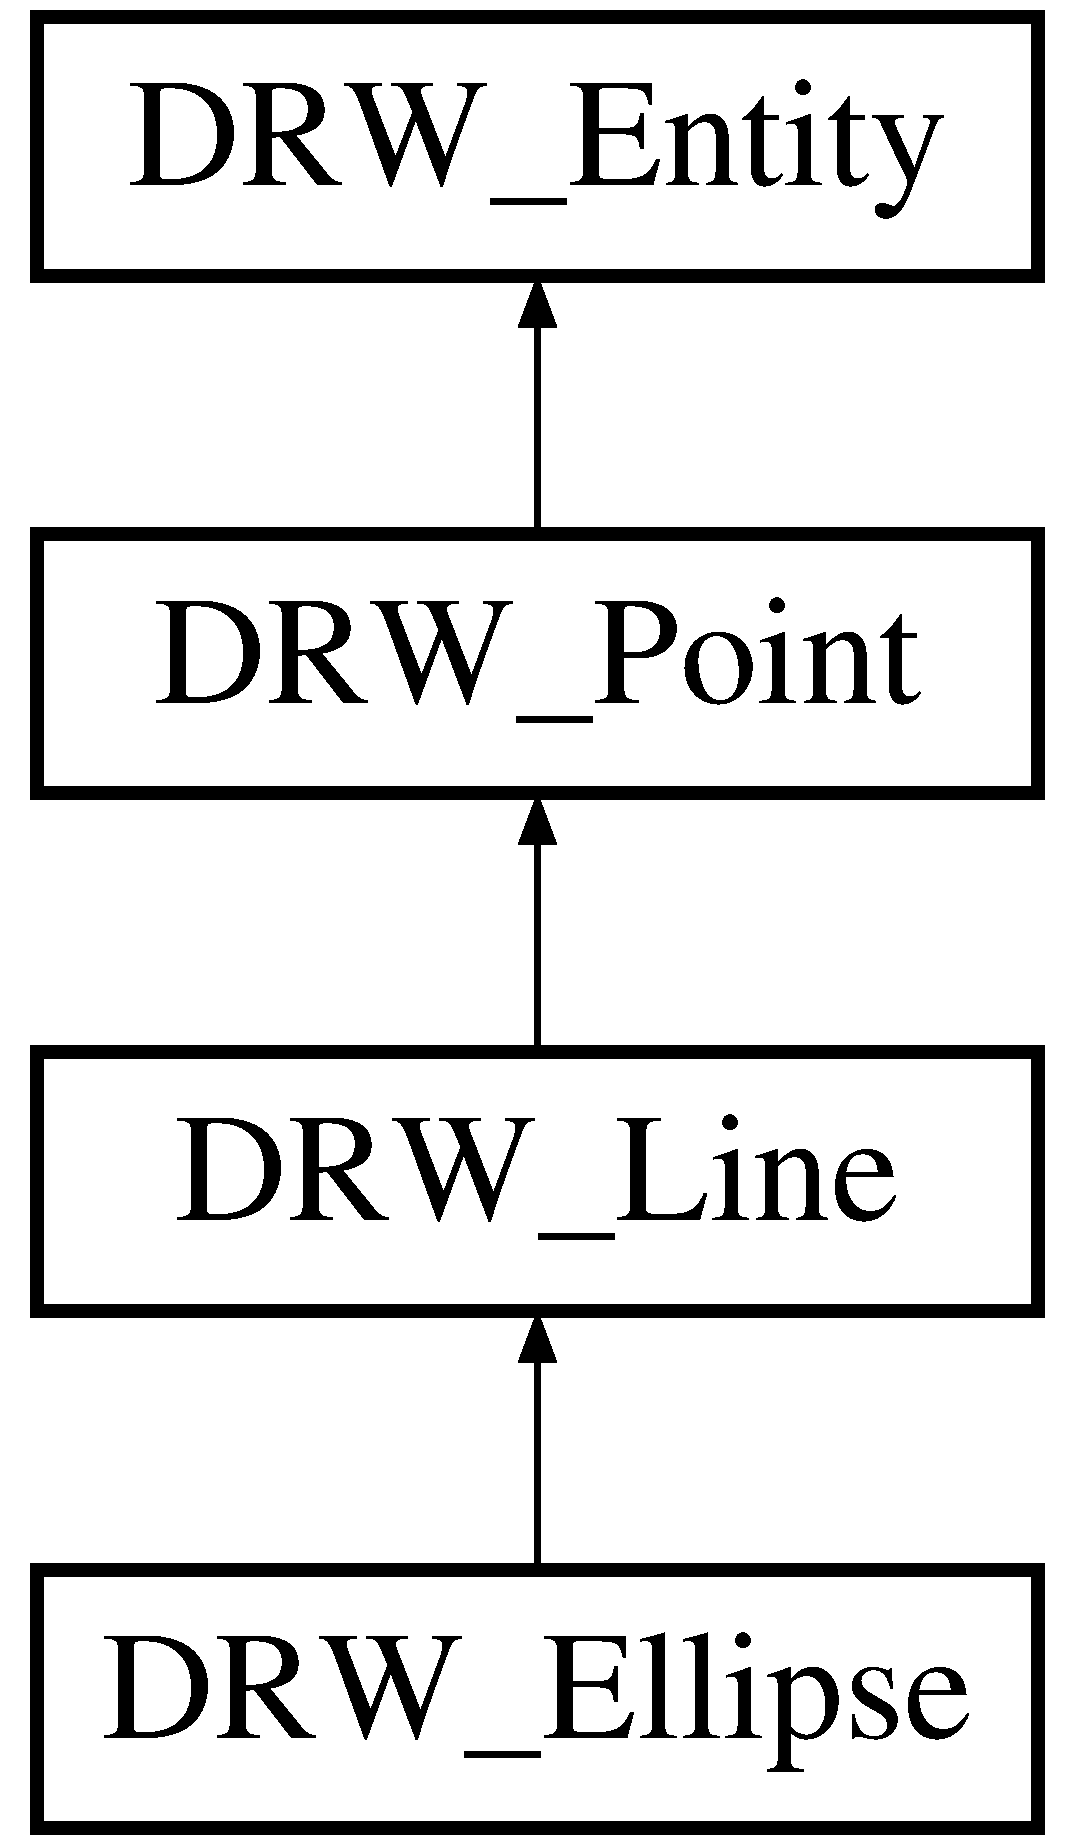
\includegraphics[height=4.000000cm]{d0/ded/class_d_r_w___ellipse}
\end{center}
\end{figure}
\subsection*{Public Attributes}
\begin{DoxyCompactItemize}
\item 
double \hyperlink{class_d_r_w___ellipse_a5f99577d5e97fa8e0d308a2ab52a2f95}{ratio}
\item 
double \hyperlink{class_d_r_w___ellipse_a8b9ca88b1d30755bdaa2de0e11116ede}{staparam}
\item 
double \hyperlink{class_d_r_w___ellipse_a69490d7e26d7c8fa602ef4a540b22d52}{endparam}
\item 
int \hyperlink{class_d_r_w___ellipse_a6a8cd9de5c300fde3c52c26daf66ac77}{isccw}
\end{DoxyCompactItemize}
\subsection*{Protected Member Functions}
\begin{DoxyCompactItemize}
\item 
\hypertarget{class_d_r_w___ellipse_a7e271b176d81110b92931514bddb2e6d}{}void \hyperlink{class_d_r_w___ellipse_a7e271b176d81110b92931514bddb2e6d}{parse\+Code} (int code, dxf\+Reader $\ast$reader)\label{class_d_r_w___ellipse_a7e271b176d81110b92931514bddb2e6d}

\begin{DoxyCompactList}\small\item\em interpret code in dxf reading process or dispatch to inherited class \end{DoxyCompactList}\item 
\hypertarget{class_d_r_w___ellipse_aa8871bb334eb53eb669eae505a4ae9fd}{}virtual bool \hyperlink{class_d_r_w___ellipse_aa8871bb334eb53eb669eae505a4ae9fd}{parse\+Dwg} (D\+R\+W\+::\+Version v, dwg\+Buffer $\ast$buf)\label{class_d_r_w___ellipse_aa8871bb334eb53eb669eae505a4ae9fd}

\begin{DoxyCompactList}\small\item\em interpret dwg data (was already determined to be part of this object) \end{DoxyCompactList}\end{DoxyCompactItemize}


\subsection{Detailed Description}
Class to handle ellipse entity. 

Class to handle ellipse and elliptic arc entity Note\+: start/end parameter are in radians for ellipse entity but for hatch boundary are in degrees \begin{DoxyAuthor}{Author}
Rallaz 
\end{DoxyAuthor}


\subsection{Member Data Documentation}
\hypertarget{class_d_r_w___ellipse_a69490d7e26d7c8fa602ef4a540b22d52}{}\index{D\+R\+W\+\_\+\+Ellipse@{D\+R\+W\+\_\+\+Ellipse}!endparam@{endparam}}
\index{endparam@{endparam}!D\+R\+W\+\_\+\+Ellipse@{D\+R\+W\+\_\+\+Ellipse}}
\subsubsection[{endparam}]{\setlength{\rightskip}{0pt plus 5cm}double D\+R\+W\+\_\+\+Ellipse\+::endparam}\label{class_d_r_w___ellipse_a69490d7e26d7c8fa602ef4a540b22d52}
end parameter, code 42, 2$\ast$\+P\+I for full ellipse \hypertarget{class_d_r_w___ellipse_a6a8cd9de5c300fde3c52c26daf66ac77}{}\index{D\+R\+W\+\_\+\+Ellipse@{D\+R\+W\+\_\+\+Ellipse}!isccw@{isccw}}
\index{isccw@{isccw}!D\+R\+W\+\_\+\+Ellipse@{D\+R\+W\+\_\+\+Ellipse}}
\subsubsection[{isccw}]{\setlength{\rightskip}{0pt plus 5cm}int D\+R\+W\+\_\+\+Ellipse\+::isccw}\label{class_d_r_w___ellipse_a6a8cd9de5c300fde3c52c26daf66ac77}
is counter clockwise arc?, only used in hatch, code 73 \hypertarget{class_d_r_w___ellipse_a5f99577d5e97fa8e0d308a2ab52a2f95}{}\index{D\+R\+W\+\_\+\+Ellipse@{D\+R\+W\+\_\+\+Ellipse}!ratio@{ratio}}
\index{ratio@{ratio}!D\+R\+W\+\_\+\+Ellipse@{D\+R\+W\+\_\+\+Ellipse}}
\subsubsection[{ratio}]{\setlength{\rightskip}{0pt plus 5cm}double D\+R\+W\+\_\+\+Ellipse\+::ratio}\label{class_d_r_w___ellipse_a5f99577d5e97fa8e0d308a2ab52a2f95}
ratio, code 40 \hypertarget{class_d_r_w___ellipse_a8b9ca88b1d30755bdaa2de0e11116ede}{}\index{D\+R\+W\+\_\+\+Ellipse@{D\+R\+W\+\_\+\+Ellipse}!staparam@{staparam}}
\index{staparam@{staparam}!D\+R\+W\+\_\+\+Ellipse@{D\+R\+W\+\_\+\+Ellipse}}
\subsubsection[{staparam}]{\setlength{\rightskip}{0pt plus 5cm}double D\+R\+W\+\_\+\+Ellipse\+::staparam}\label{class_d_r_w___ellipse_a8b9ca88b1d30755bdaa2de0e11116ede}
start parameter, code 41, 0.\+0 for full ellipse 

The documentation for this class was generated from the following files\+:\begin{DoxyCompactItemize}
\item 
src/drw\+\_\+entities.\+h\item 
src/drw\+\_\+entities.\+cpp\end{DoxyCompactItemize}

\hypertarget{class_d_r_w___entity}{}\section{D\+R\+W\+\_\+\+Entity Class Reference}
\label{class_d_r_w___entity}\index{D\+R\+W\+\_\+\+Entity@{D\+R\+W\+\_\+\+Entity}}


Base class for entities.  




{\ttfamily \#include $<$drw\+\_\+entities.\+h$>$}

Inheritance diagram for D\+R\+W\+\_\+\+Entity\+:\begin{figure}[H]
\begin{center}
\leavevmode
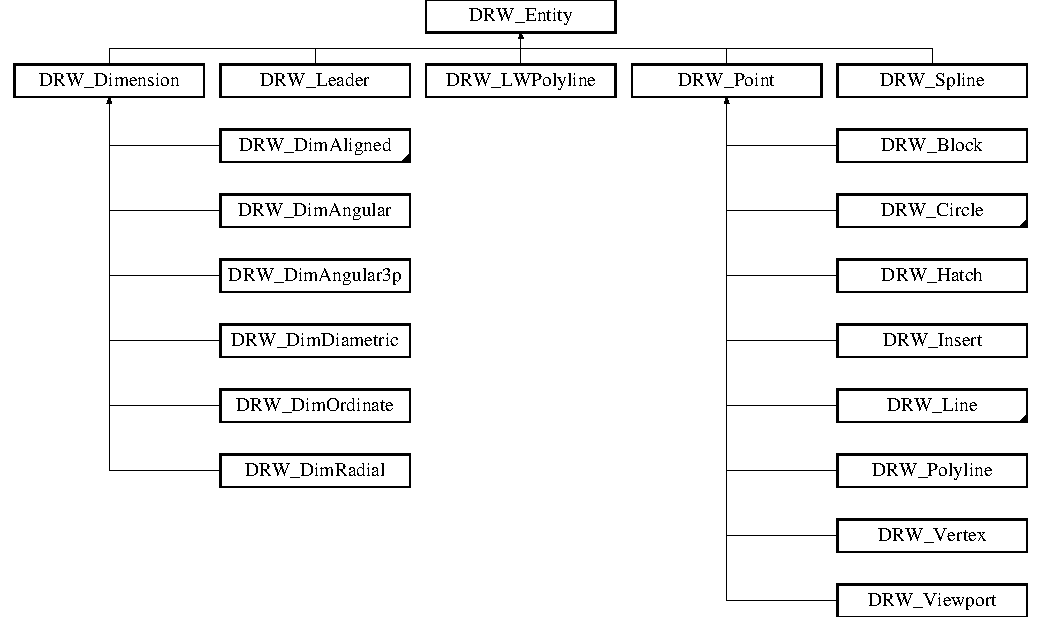
\includegraphics[height=8.296296cm]{d2/d59/class_d_r_w___entity}
\end{center}
\end{figure}
\subsection*{Public Attributes}
\begin{DoxyCompactItemize}
\item 
enum D\+R\+W\+::\+E\+T\+Y\+P\+E \hyperlink{class_d_r_w___entity_a36dff42707384984a085dbea602d0217}{e\+Type}
\item 
int \hyperlink{class_d_r_w___entity_a32f66a2b4da26f1f9a42ffa8539c916c}{handle}
\item 
duint32 \hyperlink{class_d_r_w___entity_a76823e459149440d84397803e205dd55}{handle\+Dict}
\item 
duint32 \hyperlink{class_d_r_w___entity_afb7d80168b82c574d5387c4b0aa4cdd5}{handle\+Block}
\item 
U\+T\+F8\+S\+T\+R\+I\+N\+G \hyperlink{class_d_r_w___entity_a65b68c6c8712de3e2fada1d263b96042}{layer}
\item 
U\+T\+F8\+S\+T\+R\+I\+N\+G \hyperlink{class_d_r_w___entity_a1180883df434a22fdafbc8ac1273e46e}{line\+Type}
\item 
int \hyperlink{class_d_r_w___entity_a199afc08d2cc4c44ea58d49780582526}{color}
\item 
enum \hyperlink{class_d_r_w___l_w___conv_aed68cbc3d8bdf7e20003dd2d970279b3}{D\+R\+W\+\_\+\+L\+W\+\_\+\+Conv\+::line\+Width} \hyperlink{class_d_r_w___entity_a5e01429ed3b7199b17367a5c85970a0d}{l\+Weight}
\item 
double \hyperlink{class_d_r_w___entity_a167d107e81c5b2bb4ee015fa62e2fde2}{ltype\+Scale}
\item 
bool \hyperlink{class_d_r_w___entity_a410a134f3127298598a0075e60f3616d}{visible}
\item 
int \hyperlink{class_d_r_w___entity_a4448fbdbe618f83ed71a7c1ed98caeae}{color24}
\item 
std\+::string \hyperlink{class_d_r_w___entity_a84620ae9c9eea40d9d6373f28db5877a}{color\+Name}
\item 
D\+R\+W\+::\+Space \hyperlink{class_d_r_w___entity_a8baf5455459e70a668e59fd13cfa72e2}{space}
\item 
bool \hyperlink{class_d_r_w___entity_a62545716d4aec61cabb85576afc78dee}{have\+Extrusion}
\item 
std\+::string \hyperlink{class_d_r_w___entity_a10185df2d2f4d551921332c0968652d4}{image}
\item 
D\+R\+W\+::\+Shadow\+Mode \hyperlink{class_d_r_w___entity_add69fd0a0f9ac49dfc5aca84c3023c56}{shadow}
\item 
int \hyperlink{class_d_r_w___entity_a29c774531a5109cedc01eed7f2822f76}{material}
\item 
int \hyperlink{class_d_r_w___entity_abebf612b67fe860b34163f8cc16f0e78}{plot\+Style}
\item 
int \hyperlink{class_d_r_w___entity_a3706fb94037a61f8a4b705210b136117}{transparency}
\end{DoxyCompactItemize}
\subsection*{Protected Member Functions}
\begin{DoxyCompactItemize}
\item 
void \hyperlink{class_d_r_w___entity_a84d72c116d6bfaf0b1dab2782b8a764b}{calculate\+Axis} (\hyperlink{class_d_r_w___coord}{D\+R\+W\+\_\+\+Coord} ext\+Point)
\begin{DoxyCompactList}\small\item\em Calculate arbitary axis. \end{DoxyCompactList}\item 
void \hyperlink{class_d_r_w___entity_a1c82add778b9dc940fa8f0231287858c}{extrude\+Point} (\hyperlink{class_d_r_w___coord}{D\+R\+W\+\_\+\+Coord} ext\+Point, \hyperlink{class_d_r_w___coord}{D\+R\+W\+\_\+\+Coord} $\ast$point)
\begin{DoxyCompactList}\small\item\em Extrude a point using arbitary axis. \end{DoxyCompactList}\end{DoxyCompactItemize}


\subsection{Detailed Description}
Base class for entities. 

Base class for entities \begin{DoxyAuthor}{Author}
Rallaz 
\end{DoxyAuthor}


\subsection{Member Function Documentation}
\hypertarget{class_d_r_w___entity_a84d72c116d6bfaf0b1dab2782b8a764b}{}\index{D\+R\+W\+\_\+\+Entity@{D\+R\+W\+\_\+\+Entity}!calculate\+Axis@{calculate\+Axis}}
\index{calculate\+Axis@{calculate\+Axis}!D\+R\+W\+\_\+\+Entity@{D\+R\+W\+\_\+\+Entity}}
\subsubsection[{calculate\+Axis}]{\setlength{\rightskip}{0pt plus 5cm}void D\+R\+W\+\_\+\+Entity\+::calculate\+Axis (
\begin{DoxyParamCaption}
\item[{{\bf D\+R\+W\+\_\+\+Coord}}]{ext\+Point}
\end{DoxyParamCaption}
)\hspace{0.3cm}{\ttfamily [protected]}}\label{class_d_r_w___entity_a84d72c116d6bfaf0b1dab2782b8a764b}


Calculate arbitary axis. 

Calculate arbitary axis for apply extrusions \begin{DoxyAuthor}{Author}
Rallaz 
\end{DoxyAuthor}
\hypertarget{class_d_r_w___entity_a1c82add778b9dc940fa8f0231287858c}{}\index{D\+R\+W\+\_\+\+Entity@{D\+R\+W\+\_\+\+Entity}!extrude\+Point@{extrude\+Point}}
\index{extrude\+Point@{extrude\+Point}!D\+R\+W\+\_\+\+Entity@{D\+R\+W\+\_\+\+Entity}}
\subsubsection[{extrude\+Point}]{\setlength{\rightskip}{0pt plus 5cm}void D\+R\+W\+\_\+\+Entity\+::extrude\+Point (
\begin{DoxyParamCaption}
\item[{{\bf D\+R\+W\+\_\+\+Coord}}]{ext\+Point, }
\item[{{\bf D\+R\+W\+\_\+\+Coord} $\ast$}]{point}
\end{DoxyParamCaption}
)\hspace{0.3cm}{\ttfamily [protected]}}\label{class_d_r_w___entity_a1c82add778b9dc940fa8f0231287858c}


Extrude a point using arbitary axis. 

apply extrusion in a point using arbitary axis (previous calculated) \begin{DoxyAuthor}{Author}
Rallaz 
\end{DoxyAuthor}


\subsection{Member Data Documentation}
\hypertarget{class_d_r_w___entity_a199afc08d2cc4c44ea58d49780582526}{}\index{D\+R\+W\+\_\+\+Entity@{D\+R\+W\+\_\+\+Entity}!color@{color}}
\index{color@{color}!D\+R\+W\+\_\+\+Entity@{D\+R\+W\+\_\+\+Entity}}
\subsubsection[{color}]{\setlength{\rightskip}{0pt plus 5cm}int D\+R\+W\+\_\+\+Entity\+::color}\label{class_d_r_w___entity_a199afc08d2cc4c44ea58d49780582526}
entity color, code 62 \hypertarget{class_d_r_w___entity_a4448fbdbe618f83ed71a7c1ed98caeae}{}\index{D\+R\+W\+\_\+\+Entity@{D\+R\+W\+\_\+\+Entity}!color24@{color24}}
\index{color24@{color24}!D\+R\+W\+\_\+\+Entity@{D\+R\+W\+\_\+\+Entity}}
\subsubsection[{color24}]{\setlength{\rightskip}{0pt plus 5cm}int D\+R\+W\+\_\+\+Entity\+::color24}\label{class_d_r_w___entity_a4448fbdbe618f83ed71a7c1ed98caeae}
24-\/bit color, code 420 \hypertarget{class_d_r_w___entity_a84620ae9c9eea40d9d6373f28db5877a}{}\index{D\+R\+W\+\_\+\+Entity@{D\+R\+W\+\_\+\+Entity}!color\+Name@{color\+Name}}
\index{color\+Name@{color\+Name}!D\+R\+W\+\_\+\+Entity@{D\+R\+W\+\_\+\+Entity}}
\subsubsection[{color\+Name}]{\setlength{\rightskip}{0pt plus 5cm}std\+::string D\+R\+W\+\_\+\+Entity\+::color\+Name}\label{class_d_r_w___entity_a84620ae9c9eea40d9d6373f28db5877a}
color name, code 430 \hypertarget{class_d_r_w___entity_a36dff42707384984a085dbea602d0217}{}\index{D\+R\+W\+\_\+\+Entity@{D\+R\+W\+\_\+\+Entity}!e\+Type@{e\+Type}}
\index{e\+Type@{e\+Type}!D\+R\+W\+\_\+\+Entity@{D\+R\+W\+\_\+\+Entity}}
\subsubsection[{e\+Type}]{\setlength{\rightskip}{0pt plus 5cm}enum D\+R\+W\+::\+E\+T\+Y\+P\+E D\+R\+W\+\_\+\+Entity\+::e\+Type}\label{class_d_r_w___entity_a36dff42707384984a085dbea602d0217}
enum\+: entity type, code 0 \hypertarget{class_d_r_w___entity_a32f66a2b4da26f1f9a42ffa8539c916c}{}\index{D\+R\+W\+\_\+\+Entity@{D\+R\+W\+\_\+\+Entity}!handle@{handle}}
\index{handle@{handle}!D\+R\+W\+\_\+\+Entity@{D\+R\+W\+\_\+\+Entity}}
\subsubsection[{handle}]{\setlength{\rightskip}{0pt plus 5cm}int D\+R\+W\+\_\+\+Entity\+::handle}\label{class_d_r_w___entity_a32f66a2b4da26f1f9a42ffa8539c916c}
entity identifier, code 5 \hypertarget{class_d_r_w___entity_afb7d80168b82c574d5387c4b0aa4cdd5}{}\index{D\+R\+W\+\_\+\+Entity@{D\+R\+W\+\_\+\+Entity}!handle\+Block@{handle\+Block}}
\index{handle\+Block@{handle\+Block}!D\+R\+W\+\_\+\+Entity@{D\+R\+W\+\_\+\+Entity}}
\subsubsection[{handle\+Block}]{\setlength{\rightskip}{0pt plus 5cm}duint32 D\+R\+W\+\_\+\+Entity\+::handle\+Block}\label{class_d_r_w___entity_afb7d80168b82c574d5387c4b0aa4cdd5}
Soft-\/pointer I\+D/handle to owner B\+L\+O\+C\+K\+\_\+\+R\+E\+C\+O\+R\+D object, code 330 \hypertarget{class_d_r_w___entity_a76823e459149440d84397803e205dd55}{}\index{D\+R\+W\+\_\+\+Entity@{D\+R\+W\+\_\+\+Entity}!handle\+Dict@{handle\+Dict}}
\index{handle\+Dict@{handle\+Dict}!D\+R\+W\+\_\+\+Entity@{D\+R\+W\+\_\+\+Entity}}
\subsubsection[{handle\+Dict}]{\setlength{\rightskip}{0pt plus 5cm}duint32 D\+R\+W\+\_\+\+Entity\+::handle\+Dict}\label{class_d_r_w___entity_a76823e459149440d84397803e205dd55}
Hard-\/pointer I\+D/handle to owner dictionary, code 360 \hypertarget{class_d_r_w___entity_a62545716d4aec61cabb85576afc78dee}{}\index{D\+R\+W\+\_\+\+Entity@{D\+R\+W\+\_\+\+Entity}!have\+Extrusion@{have\+Extrusion}}
\index{have\+Extrusion@{have\+Extrusion}!D\+R\+W\+\_\+\+Entity@{D\+R\+W\+\_\+\+Entity}}
\subsubsection[{have\+Extrusion}]{\setlength{\rightskip}{0pt plus 5cm}bool D\+R\+W\+\_\+\+Entity\+::have\+Extrusion}\label{class_d_r_w___entity_a62545716d4aec61cabb85576afc78dee}
set to true if the entity have extrusion \hypertarget{class_d_r_w___entity_a10185df2d2f4d551921332c0968652d4}{}\index{D\+R\+W\+\_\+\+Entity@{D\+R\+W\+\_\+\+Entity}!image@{image}}
\index{image@{image}!D\+R\+W\+\_\+\+Entity@{D\+R\+W\+\_\+\+Entity}}
\subsubsection[{image}]{\setlength{\rightskip}{0pt plus 5cm}std\+::string D\+R\+W\+\_\+\+Entity\+::image}\label{class_d_r_w___entity_a10185df2d2f4d551921332c0968652d4}
proxy entity graphics, code 92 and 310 \hypertarget{class_d_r_w___entity_a65b68c6c8712de3e2fada1d263b96042}{}\index{D\+R\+W\+\_\+\+Entity@{D\+R\+W\+\_\+\+Entity}!layer@{layer}}
\index{layer@{layer}!D\+R\+W\+\_\+\+Entity@{D\+R\+W\+\_\+\+Entity}}
\subsubsection[{layer}]{\setlength{\rightskip}{0pt plus 5cm}U\+T\+F8\+S\+T\+R\+I\+N\+G D\+R\+W\+\_\+\+Entity\+::layer}\label{class_d_r_w___entity_a65b68c6c8712de3e2fada1d263b96042}
layer name, code 8 \hypertarget{class_d_r_w___entity_a1180883df434a22fdafbc8ac1273e46e}{}\index{D\+R\+W\+\_\+\+Entity@{D\+R\+W\+\_\+\+Entity}!line\+Type@{line\+Type}}
\index{line\+Type@{line\+Type}!D\+R\+W\+\_\+\+Entity@{D\+R\+W\+\_\+\+Entity}}
\subsubsection[{line\+Type}]{\setlength{\rightskip}{0pt plus 5cm}U\+T\+F8\+S\+T\+R\+I\+N\+G D\+R\+W\+\_\+\+Entity\+::line\+Type}\label{class_d_r_w___entity_a1180883df434a22fdafbc8ac1273e46e}
line type, code 6 \hypertarget{class_d_r_w___entity_a167d107e81c5b2bb4ee015fa62e2fde2}{}\index{D\+R\+W\+\_\+\+Entity@{D\+R\+W\+\_\+\+Entity}!ltype\+Scale@{ltype\+Scale}}
\index{ltype\+Scale@{ltype\+Scale}!D\+R\+W\+\_\+\+Entity@{D\+R\+W\+\_\+\+Entity}}
\subsubsection[{ltype\+Scale}]{\setlength{\rightskip}{0pt plus 5cm}double D\+R\+W\+\_\+\+Entity\+::ltype\+Scale}\label{class_d_r_w___entity_a167d107e81c5b2bb4ee015fa62e2fde2}
linetype scale, code 48 \hypertarget{class_d_r_w___entity_a5e01429ed3b7199b17367a5c85970a0d}{}\index{D\+R\+W\+\_\+\+Entity@{D\+R\+W\+\_\+\+Entity}!l\+Weight@{l\+Weight}}
\index{l\+Weight@{l\+Weight}!D\+R\+W\+\_\+\+Entity@{D\+R\+W\+\_\+\+Entity}}
\subsubsection[{l\+Weight}]{\setlength{\rightskip}{0pt plus 5cm}enum {\bf D\+R\+W\+\_\+\+L\+W\+\_\+\+Conv\+::line\+Width} D\+R\+W\+\_\+\+Entity\+::l\+Weight}\label{class_d_r_w___entity_a5e01429ed3b7199b17367a5c85970a0d}
entity lineweight, code 370 \hypertarget{class_d_r_w___entity_a29c774531a5109cedc01eed7f2822f76}{}\index{D\+R\+W\+\_\+\+Entity@{D\+R\+W\+\_\+\+Entity}!material@{material}}
\index{material@{material}!D\+R\+W\+\_\+\+Entity@{D\+R\+W\+\_\+\+Entity}}
\subsubsection[{material}]{\setlength{\rightskip}{0pt plus 5cm}int D\+R\+W\+\_\+\+Entity\+::material}\label{class_d_r_w___entity_a29c774531a5109cedc01eed7f2822f76}
hard pointer id to material object, code 347 \hypertarget{class_d_r_w___entity_abebf612b67fe860b34163f8cc16f0e78}{}\index{D\+R\+W\+\_\+\+Entity@{D\+R\+W\+\_\+\+Entity}!plot\+Style@{plot\+Style}}
\index{plot\+Style@{plot\+Style}!D\+R\+W\+\_\+\+Entity@{D\+R\+W\+\_\+\+Entity}}
\subsubsection[{plot\+Style}]{\setlength{\rightskip}{0pt plus 5cm}int D\+R\+W\+\_\+\+Entity\+::plot\+Style}\label{class_d_r_w___entity_abebf612b67fe860b34163f8cc16f0e78}
hard pointer id to plot style object, code 420 \hypertarget{class_d_r_w___entity_add69fd0a0f9ac49dfc5aca84c3023c56}{}\index{D\+R\+W\+\_\+\+Entity@{D\+R\+W\+\_\+\+Entity}!shadow@{shadow}}
\index{shadow@{shadow}!D\+R\+W\+\_\+\+Entity@{D\+R\+W\+\_\+\+Entity}}
\subsubsection[{shadow}]{\setlength{\rightskip}{0pt plus 5cm}D\+R\+W\+::\+Shadow\+Mode D\+R\+W\+\_\+\+Entity\+::shadow}\label{class_d_r_w___entity_add69fd0a0f9ac49dfc5aca84c3023c56}
shadow mode, code 284 \hypertarget{class_d_r_w___entity_a8baf5455459e70a668e59fd13cfa72e2}{}\index{D\+R\+W\+\_\+\+Entity@{D\+R\+W\+\_\+\+Entity}!space@{space}}
\index{space@{space}!D\+R\+W\+\_\+\+Entity@{D\+R\+W\+\_\+\+Entity}}
\subsubsection[{space}]{\setlength{\rightskip}{0pt plus 5cm}D\+R\+W\+::\+Space D\+R\+W\+\_\+\+Entity\+::space}\label{class_d_r_w___entity_a8baf5455459e70a668e59fd13cfa72e2}
space indicator, code 67 \hypertarget{class_d_r_w___entity_a3706fb94037a61f8a4b705210b136117}{}\index{D\+R\+W\+\_\+\+Entity@{D\+R\+W\+\_\+\+Entity}!transparency@{transparency}}
\index{transparency@{transparency}!D\+R\+W\+\_\+\+Entity@{D\+R\+W\+\_\+\+Entity}}
\subsubsection[{transparency}]{\setlength{\rightskip}{0pt plus 5cm}int D\+R\+W\+\_\+\+Entity\+::transparency}\label{class_d_r_w___entity_a3706fb94037a61f8a4b705210b136117}
transparency, code 440 \hypertarget{class_d_r_w___entity_a410a134f3127298598a0075e60f3616d}{}\index{D\+R\+W\+\_\+\+Entity@{D\+R\+W\+\_\+\+Entity}!visible@{visible}}
\index{visible@{visible}!D\+R\+W\+\_\+\+Entity@{D\+R\+W\+\_\+\+Entity}}
\subsubsection[{visible}]{\setlength{\rightskip}{0pt plus 5cm}bool D\+R\+W\+\_\+\+Entity\+::visible}\label{class_d_r_w___entity_a410a134f3127298598a0075e60f3616d}
entity visibility, code 60 

The documentation for this class was generated from the following files\+:\begin{DoxyCompactItemize}
\item 
src/drw\+\_\+entities.\+h\item 
src/drw\+\_\+entities.\+cpp\end{DoxyCompactItemize}

\hypertarget{class_d_r_w___hatch}{}\section{D\+R\+W\+\_\+\+Hatch Class Reference}
\label{class_d_r_w___hatch}\index{D\+R\+W\+\_\+\+Hatch@{D\+R\+W\+\_\+\+Hatch}}


Class to handle hatch entity.  




{\ttfamily \#include $<$drw\+\_\+entities.\+h$>$}

Inheritance diagram for D\+R\+W\+\_\+\+Hatch\+:\begin{figure}[H]
\begin{center}
\leavevmode
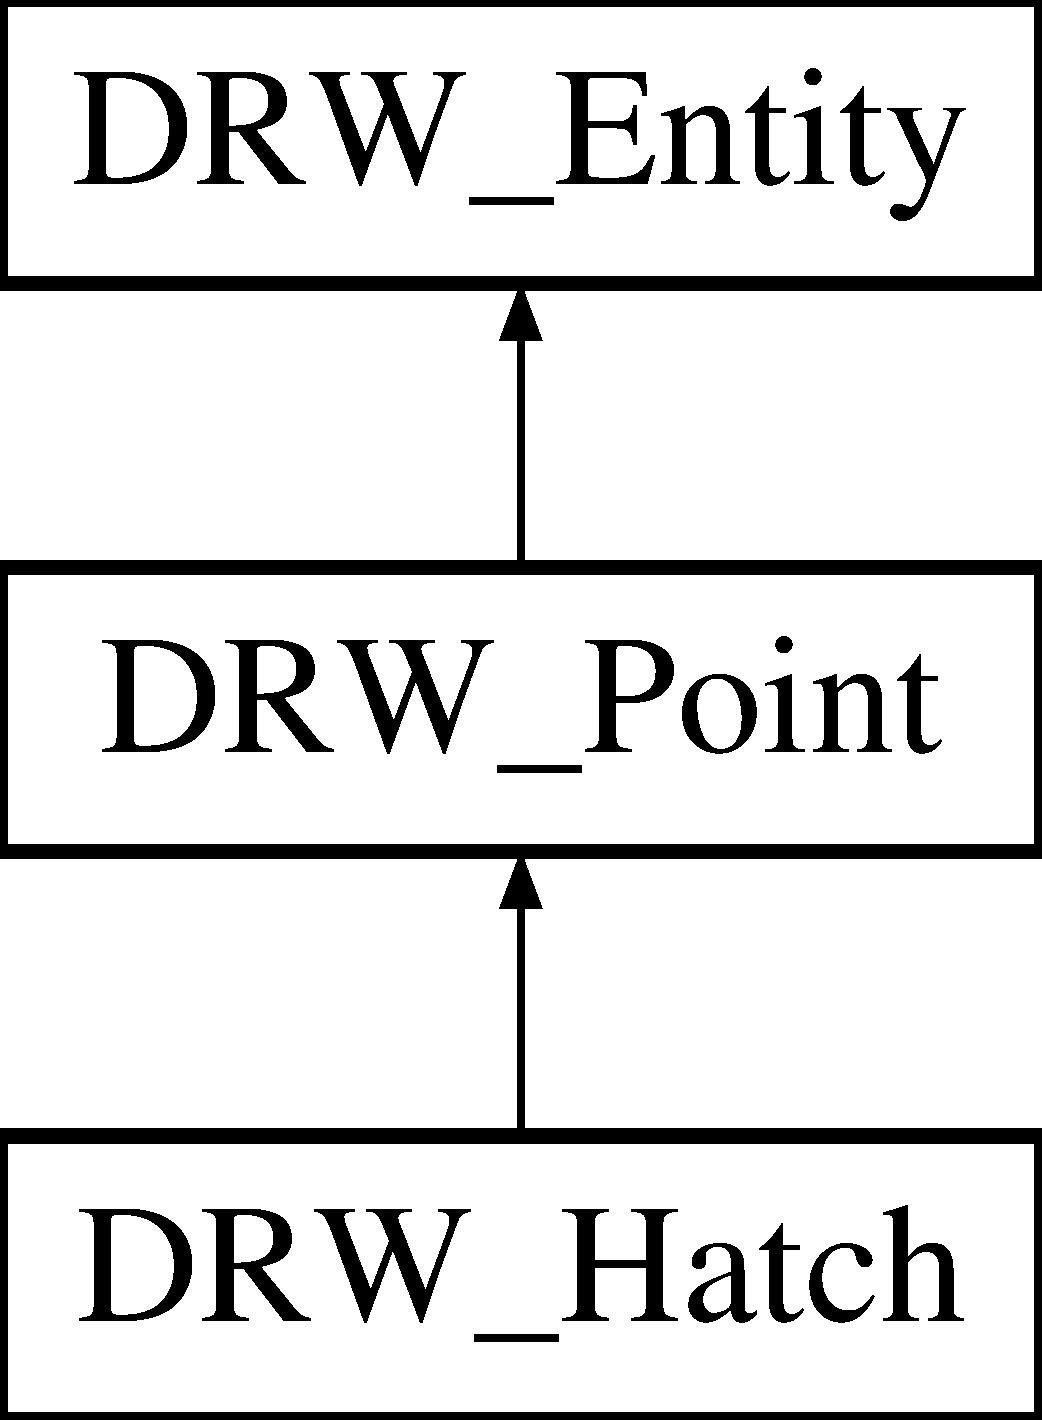
\includegraphics[height=3.000000cm]{d1/d3e/class_d_r_w___hatch}
\end{center}
\end{figure}
\subsection*{Public Attributes}
\begin{DoxyCompactItemize}
\item 
U\+T\+F8\+S\+T\+R\+I\+N\+G \hyperlink{class_d_r_w___hatch_a3e864b79a0757b7ab2a8c32a21165150}{name}
\item 
int \hyperlink{class_d_r_w___hatch_a4eec0fc3cd839a3892e875bcc9789d48}{solid}
\item 
int \hyperlink{class_d_r_w___hatch_af152cba96e8bd0471aafd2764defe458}{associative}
\item 
int \hyperlink{class_d_r_w___hatch_a7b8950911e5fb319f0d63b7ee2251f87}{hstyle}
\item 
int \hyperlink{class_d_r_w___hatch_abb23290d594b69e7b9c18ece2de7ec8e}{hpattern}
\item 
int \hyperlink{class_d_r_w___hatch_a06da8a64445bd9e5c159dab4243c992a}{doubleflag}
\item 
int \hyperlink{class_d_r_w___hatch_a52ba4f38bba83fe735cb14447e256260}{loopsnum}
\item 
double \hyperlink{class_d_r_w___hatch_aee22d8d574a33e852ad82c345899b886}{angle}
\item 
double \hyperlink{class_d_r_w___hatch_a0ee3311f6d41385488af2cafd55cd7ef}{scale}
\item 
int \hyperlink{class_d_r_w___hatch_a15bd241e3c34d82c35db31470fe25741}{deflines}
\item 
std\+::vector$<$ \hyperlink{class_d_r_w___hatch_loop}{D\+R\+W\+\_\+\+Hatch\+Loop} $\ast$ $>$ \hyperlink{class_d_r_w___hatch_a258a13a2da31ae31fd22e2da3757da5c}{looplist}
\end{DoxyCompactItemize}
\subsection*{Private Attributes}
\begin{DoxyCompactItemize}
\item 
\hyperlink{class_d_r_w___hatch_loop}{D\+R\+W\+\_\+\+Hatch\+Loop} $\ast$ \hyperlink{class_d_r_w___hatch_a2da61f1c2549cf8dacd0a0bb13366d56}{loop}
\end{DoxyCompactItemize}
\subsection*{Friends}
\begin{DoxyCompactItemize}
\item 
\hypertarget{class_d_r_w___hatch_a7f080e77e5112f8364c61b97387f8ee2}{}class {\bfseries dxf\+R\+W}\label{class_d_r_w___hatch_a7f080e77e5112f8364c61b97387f8ee2}

\end{DoxyCompactItemize}
\subsection*{Additional Inherited Members}


\subsection{Detailed Description}
Class to handle hatch entity. 

Class to handle hatch entity \begin{DoxyAuthor}{Author}
Rallaz 
\end{DoxyAuthor}


\subsection{Member Data Documentation}
\hypertarget{class_d_r_w___hatch_aee22d8d574a33e852ad82c345899b886}{}\index{D\+R\+W\+\_\+\+Hatch@{D\+R\+W\+\_\+\+Hatch}!angle@{angle}}
\index{angle@{angle}!D\+R\+W\+\_\+\+Hatch@{D\+R\+W\+\_\+\+Hatch}}
\subsubsection[{angle}]{\setlength{\rightskip}{0pt plus 5cm}double D\+R\+W\+\_\+\+Hatch\+::angle}\label{class_d_r_w___hatch_aee22d8d574a33e852ad82c345899b886}
hatch pattern angle, code 52 \hypertarget{class_d_r_w___hatch_af152cba96e8bd0471aafd2764defe458}{}\index{D\+R\+W\+\_\+\+Hatch@{D\+R\+W\+\_\+\+Hatch}!associative@{associative}}
\index{associative@{associative}!D\+R\+W\+\_\+\+Hatch@{D\+R\+W\+\_\+\+Hatch}}
\subsubsection[{associative}]{\setlength{\rightskip}{0pt plus 5cm}int D\+R\+W\+\_\+\+Hatch\+::associative}\label{class_d_r_w___hatch_af152cba96e8bd0471aafd2764defe458}
associativity, code 71, associatve=1, non-\/assoc.=0 \hypertarget{class_d_r_w___hatch_a15bd241e3c34d82c35db31470fe25741}{}\index{D\+R\+W\+\_\+\+Hatch@{D\+R\+W\+\_\+\+Hatch}!deflines@{deflines}}
\index{deflines@{deflines}!D\+R\+W\+\_\+\+Hatch@{D\+R\+W\+\_\+\+Hatch}}
\subsubsection[{deflines}]{\setlength{\rightskip}{0pt plus 5cm}int D\+R\+W\+\_\+\+Hatch\+::deflines}\label{class_d_r_w___hatch_a15bd241e3c34d82c35db31470fe25741}
number of pattern definition lines, code 78 \hypertarget{class_d_r_w___hatch_a06da8a64445bd9e5c159dab4243c992a}{}\index{D\+R\+W\+\_\+\+Hatch@{D\+R\+W\+\_\+\+Hatch}!doubleflag@{doubleflag}}
\index{doubleflag@{doubleflag}!D\+R\+W\+\_\+\+Hatch@{D\+R\+W\+\_\+\+Hatch}}
\subsubsection[{doubleflag}]{\setlength{\rightskip}{0pt plus 5cm}int D\+R\+W\+\_\+\+Hatch\+::doubleflag}\label{class_d_r_w___hatch_a06da8a64445bd9e5c159dab4243c992a}
hatch pattern double flag, code 77, double=1, single=0 \hypertarget{class_d_r_w___hatch_abb23290d594b69e7b9c18ece2de7ec8e}{}\index{D\+R\+W\+\_\+\+Hatch@{D\+R\+W\+\_\+\+Hatch}!hpattern@{hpattern}}
\index{hpattern@{hpattern}!D\+R\+W\+\_\+\+Hatch@{D\+R\+W\+\_\+\+Hatch}}
\subsubsection[{hpattern}]{\setlength{\rightskip}{0pt plus 5cm}int D\+R\+W\+\_\+\+Hatch\+::hpattern}\label{class_d_r_w___hatch_abb23290d594b69e7b9c18ece2de7ec8e}
hatch pattern type, code 76 \hypertarget{class_d_r_w___hatch_a7b8950911e5fb319f0d63b7ee2251f87}{}\index{D\+R\+W\+\_\+\+Hatch@{D\+R\+W\+\_\+\+Hatch}!hstyle@{hstyle}}
\index{hstyle@{hstyle}!D\+R\+W\+\_\+\+Hatch@{D\+R\+W\+\_\+\+Hatch}}
\subsubsection[{hstyle}]{\setlength{\rightskip}{0pt plus 5cm}int D\+R\+W\+\_\+\+Hatch\+::hstyle}\label{class_d_r_w___hatch_a7b8950911e5fb319f0d63b7ee2251f87}
hatch style, code 75 \hypertarget{class_d_r_w___hatch_a2da61f1c2549cf8dacd0a0bb13366d56}{}\index{D\+R\+W\+\_\+\+Hatch@{D\+R\+W\+\_\+\+Hatch}!loop@{loop}}
\index{loop@{loop}!D\+R\+W\+\_\+\+Hatch@{D\+R\+W\+\_\+\+Hatch}}
\subsubsection[{loop}]{\setlength{\rightskip}{0pt plus 5cm}{\bf D\+R\+W\+\_\+\+Hatch\+Loop}$\ast$ D\+R\+W\+\_\+\+Hatch\+::loop\hspace{0.3cm}{\ttfamily [private]}}\label{class_d_r_w___hatch_a2da61f1c2549cf8dacd0a0bb13366d56}
current loop to add data \hypertarget{class_d_r_w___hatch_a258a13a2da31ae31fd22e2da3757da5c}{}\index{D\+R\+W\+\_\+\+Hatch@{D\+R\+W\+\_\+\+Hatch}!looplist@{looplist}}
\index{looplist@{looplist}!D\+R\+W\+\_\+\+Hatch@{D\+R\+W\+\_\+\+Hatch}}
\subsubsection[{looplist}]{\setlength{\rightskip}{0pt plus 5cm}std\+::vector$<${\bf D\+R\+W\+\_\+\+Hatch\+Loop} $\ast$$>$ D\+R\+W\+\_\+\+Hatch\+::looplist}\label{class_d_r_w___hatch_a258a13a2da31ae31fd22e2da3757da5c}
polyline list \hypertarget{class_d_r_w___hatch_a52ba4f38bba83fe735cb14447e256260}{}\index{D\+R\+W\+\_\+\+Hatch@{D\+R\+W\+\_\+\+Hatch}!loopsnum@{loopsnum}}
\index{loopsnum@{loopsnum}!D\+R\+W\+\_\+\+Hatch@{D\+R\+W\+\_\+\+Hatch}}
\subsubsection[{loopsnum}]{\setlength{\rightskip}{0pt plus 5cm}int D\+R\+W\+\_\+\+Hatch\+::loopsnum}\label{class_d_r_w___hatch_a52ba4f38bba83fe735cb14447e256260}
namber of boundary paths (loops), code 91 \hypertarget{class_d_r_w___hatch_a3e864b79a0757b7ab2a8c32a21165150}{}\index{D\+R\+W\+\_\+\+Hatch@{D\+R\+W\+\_\+\+Hatch}!name@{name}}
\index{name@{name}!D\+R\+W\+\_\+\+Hatch@{D\+R\+W\+\_\+\+Hatch}}
\subsubsection[{name}]{\setlength{\rightskip}{0pt plus 5cm}U\+T\+F8\+S\+T\+R\+I\+N\+G D\+R\+W\+\_\+\+Hatch\+::name}\label{class_d_r_w___hatch_a3e864b79a0757b7ab2a8c32a21165150}
hatch pattern name, code 2 \hypertarget{class_d_r_w___hatch_a0ee3311f6d41385488af2cafd55cd7ef}{}\index{D\+R\+W\+\_\+\+Hatch@{D\+R\+W\+\_\+\+Hatch}!scale@{scale}}
\index{scale@{scale}!D\+R\+W\+\_\+\+Hatch@{D\+R\+W\+\_\+\+Hatch}}
\subsubsection[{scale}]{\setlength{\rightskip}{0pt plus 5cm}double D\+R\+W\+\_\+\+Hatch\+::scale}\label{class_d_r_w___hatch_a0ee3311f6d41385488af2cafd55cd7ef}
hatch pattern scale, code 41 \hypertarget{class_d_r_w___hatch_a4eec0fc3cd839a3892e875bcc9789d48}{}\index{D\+R\+W\+\_\+\+Hatch@{D\+R\+W\+\_\+\+Hatch}!solid@{solid}}
\index{solid@{solid}!D\+R\+W\+\_\+\+Hatch@{D\+R\+W\+\_\+\+Hatch}}
\subsubsection[{solid}]{\setlength{\rightskip}{0pt plus 5cm}int D\+R\+W\+\_\+\+Hatch\+::solid}\label{class_d_r_w___hatch_a4eec0fc3cd839a3892e875bcc9789d48}
solid fill flag, code 70, solid=1, pattern=0 

The documentation for this class was generated from the following files\+:\begin{DoxyCompactItemize}
\item 
src/drw\+\_\+entities.\+h\item 
src/drw\+\_\+entities.\+cpp\end{DoxyCompactItemize}

\hypertarget{class_d_r_w___hatch_loop}{}\section{D\+R\+W\+\_\+\+Hatch\+Loop Class Reference}
\label{class_d_r_w___hatch_loop}\index{D\+R\+W\+\_\+\+Hatch\+Loop@{D\+R\+W\+\_\+\+Hatch\+Loop}}


Class to handle hatch loop.  




{\ttfamily \#include $<$drw\+\_\+entities.\+h$>$}

\subsection*{Public Attributes}
\begin{DoxyCompactItemize}
\item 
int \hyperlink{class_d_r_w___hatch_loop_a5891fcfa111b70221bc04c629bd6286d}{type}
\item 
int \hyperlink{class_d_r_w___hatch_loop_a48586ffbf48389a849e47c7d2412a280}{numedges}
\item 
std\+::vector$<$ \hyperlink{class_d_r_w___entity}{D\+R\+W\+\_\+\+Entity} $\ast$ $>$ \hyperlink{class_d_r_w___hatch_loop_afbd7d0876386234348fa0a301051d601}{objlist}
\end{DoxyCompactItemize}


\subsection{Detailed Description}
Class to handle hatch loop. 

Class to handle hatch loop \begin{DoxyAuthor}{Author}
Rallaz 
\end{DoxyAuthor}


\subsection{Member Data Documentation}
\hypertarget{class_d_r_w___hatch_loop_a48586ffbf48389a849e47c7d2412a280}{}\index{D\+R\+W\+\_\+\+Hatch\+Loop@{D\+R\+W\+\_\+\+Hatch\+Loop}!numedges@{numedges}}
\index{numedges@{numedges}!D\+R\+W\+\_\+\+Hatch\+Loop@{D\+R\+W\+\_\+\+Hatch\+Loop}}
\subsubsection[{numedges}]{\setlength{\rightskip}{0pt plus 5cm}int D\+R\+W\+\_\+\+Hatch\+Loop\+::numedges}\label{class_d_r_w___hatch_loop_a48586ffbf48389a849e47c7d2412a280}
number of edges (if not a polyline), code 93 \hypertarget{class_d_r_w___hatch_loop_afbd7d0876386234348fa0a301051d601}{}\index{D\+R\+W\+\_\+\+Hatch\+Loop@{D\+R\+W\+\_\+\+Hatch\+Loop}!objlist@{objlist}}
\index{objlist@{objlist}!D\+R\+W\+\_\+\+Hatch\+Loop@{D\+R\+W\+\_\+\+Hatch\+Loop}}
\subsubsection[{objlist}]{\setlength{\rightskip}{0pt plus 5cm}std\+::vector$<${\bf D\+R\+W\+\_\+\+Entity} $\ast$$>$ D\+R\+W\+\_\+\+Hatch\+Loop\+::objlist}\label{class_d_r_w___hatch_loop_afbd7d0876386234348fa0a301051d601}
entities list \hypertarget{class_d_r_w___hatch_loop_a5891fcfa111b70221bc04c629bd6286d}{}\index{D\+R\+W\+\_\+\+Hatch\+Loop@{D\+R\+W\+\_\+\+Hatch\+Loop}!type@{type}}
\index{type@{type}!D\+R\+W\+\_\+\+Hatch\+Loop@{D\+R\+W\+\_\+\+Hatch\+Loop}}
\subsubsection[{type}]{\setlength{\rightskip}{0pt plus 5cm}int D\+R\+W\+\_\+\+Hatch\+Loop\+::type}\label{class_d_r_w___hatch_loop_a5891fcfa111b70221bc04c629bd6286d}
boundary path type, code 92, polyline=2, default=0 

The documentation for this class was generated from the following file\+:\begin{DoxyCompactItemize}
\item 
src/drw\+\_\+entities.\+h\end{DoxyCompactItemize}

\hypertarget{class_d_r_w___header}{}\section{D\+R\+W\+\_\+\+Header Class Reference}
\label{class_d_r_w___header}\index{D\+R\+W\+\_\+\+Header@{D\+R\+W\+\_\+\+Header}}


Class to handle header entries.  




{\ttfamily \#include $<$drw\+\_\+header.\+h$>$}



\subsection{Detailed Description}
Class to handle header entries. 

Class to handle layer symbol table entries \begin{DoxyAuthor}{Author}
Rallaz 
\end{DoxyAuthor}


The documentation for this class was generated from the following files\+:\begin{DoxyCompactItemize}
\item 
src/drw\+\_\+header.\+h\item 
src/drw\+\_\+header.\+cpp\end{DoxyCompactItemize}

\hypertarget{class_d_r_w___image}{}\section{D\+R\+W\+\_\+\+Image Class Reference}
\label{class_d_r_w___image}\index{D\+R\+W\+\_\+\+Image@{D\+R\+W\+\_\+\+Image}}


Class to handle image entity.  




{\ttfamily \#include $<$drw\+\_\+entities.\+h$>$}

Inheritance diagram for D\+R\+W\+\_\+\+Image\+:\begin{figure}[H]
\begin{center}
\leavevmode
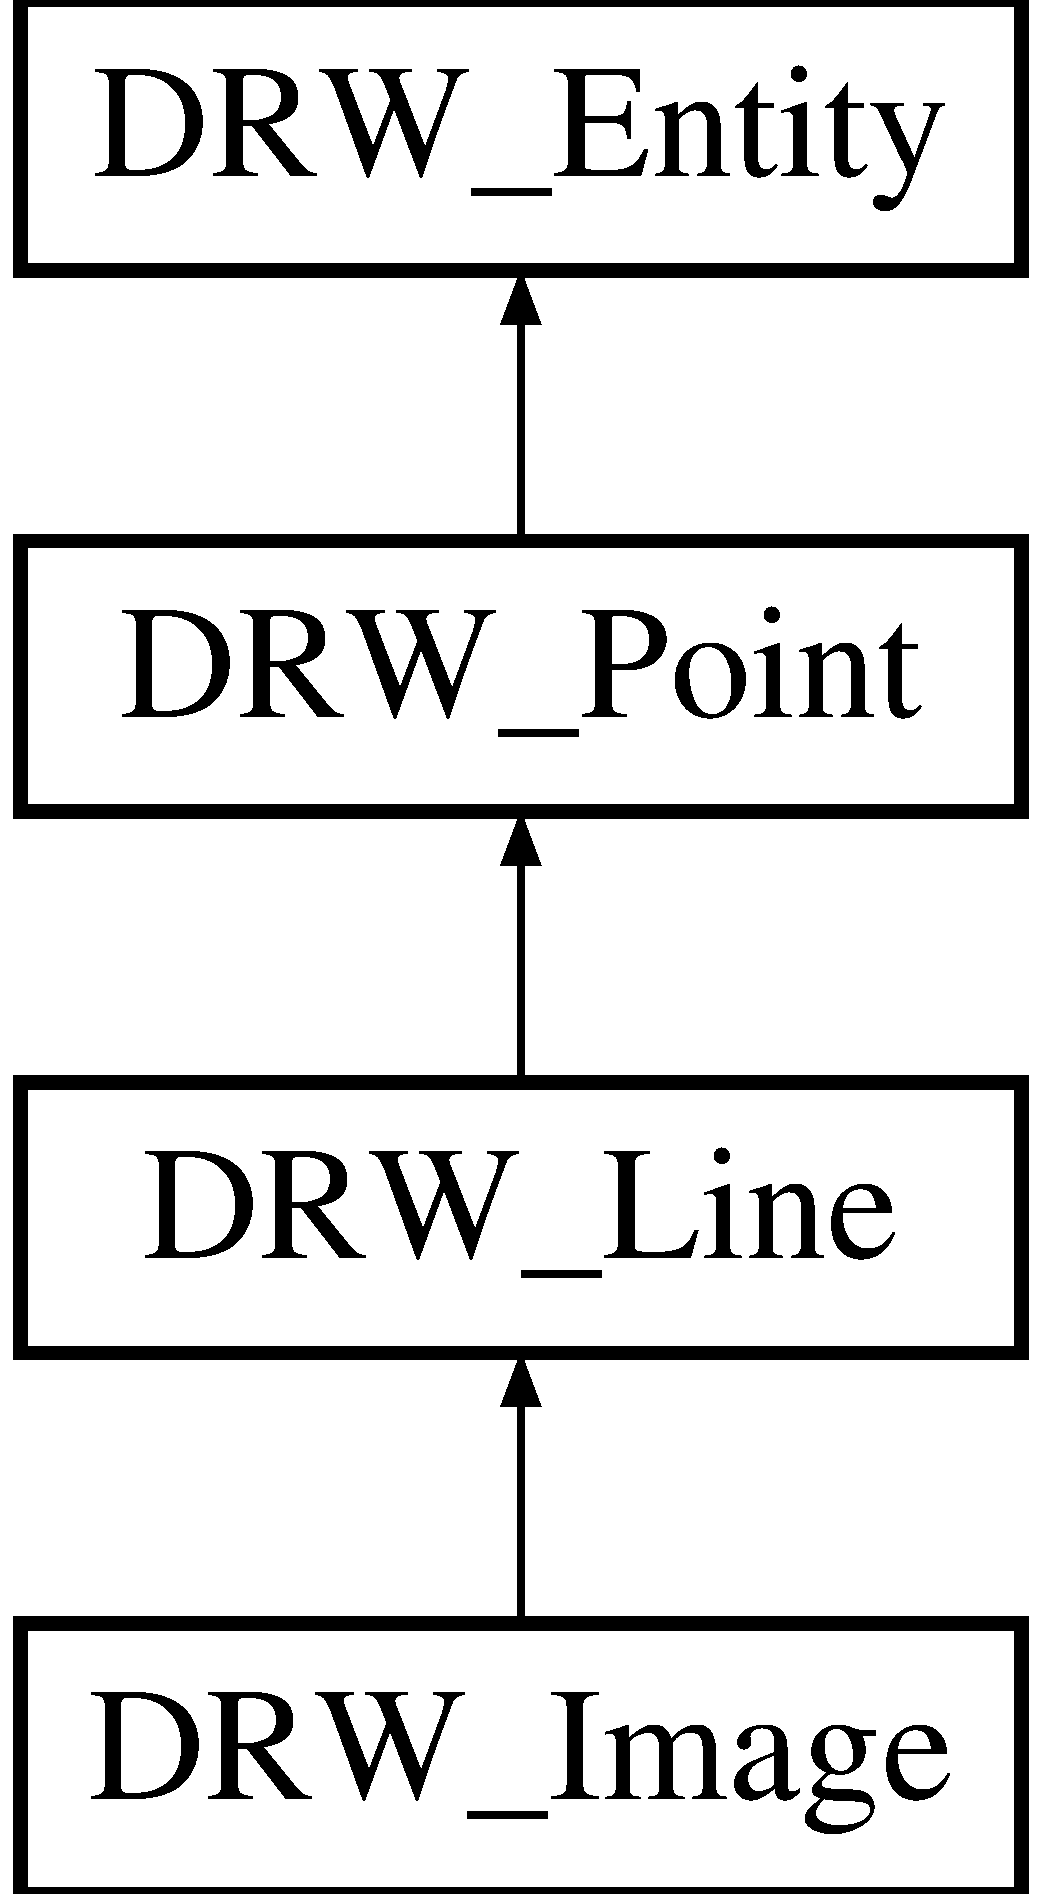
\includegraphics[height=4.000000cm]{d2/d07/class_d_r_w___image}
\end{center}
\end{figure}
\subsection*{Public Attributes}
\begin{DoxyCompactItemize}
\item 
std\+::string \hyperlink{class_d_r_w___image_a48302a8438fec582402a1c14126ffd5a}{ref}
\item 
double \hyperlink{class_d_r_w___image_a1f7b4a2b11aed54038b1e978a8d99527}{vx}
\item 
double \hyperlink{class_d_r_w___image_a955bb709e5261c3f5b3ca99bfc5765d1}{vy}
\item 
double \hyperlink{class_d_r_w___image_a075d00b1bc78bd275953d9730b0eaf8b}{vz}
\item 
double \hyperlink{class_d_r_w___image_a99a8d4b8a7fb234f002b194d0e28d247}{sizeu}
\item 
double \hyperlink{class_d_r_w___image_ae2408c33253799a6e03ea1bfec4f84d7}{sizev}
\item 
double \hyperlink{class_d_r_w___image_ada1bb1fd948f6318a4c8513e35b8224d}{dz}
\item 
int \hyperlink{class_d_r_w___image_a8d1f1854dc9b76525aa03fad3b007a58}{clip}
\item 
int \hyperlink{class_d_r_w___image_a7d088d2d2bca24de4e44cfc40e5f30bf}{brightness}
\item 
int \hyperlink{class_d_r_w___image_ad3ba08920ac1d83d073ba1f408cceb09}{contrast}
\item 
int \hyperlink{class_d_r_w___image_a29d7bf7561ed378e6f4634557aae88db}{fade}
\end{DoxyCompactItemize}
\subsection*{Friends}
\begin{DoxyCompactItemize}
\item 
\hypertarget{class_d_r_w___image_a7f080e77e5112f8364c61b97387f8ee2}{}class {\bfseries dxf\+R\+W}\label{class_d_r_w___image_a7f080e77e5112f8364c61b97387f8ee2}

\end{DoxyCompactItemize}
\subsection*{Additional Inherited Members}


\subsection{Detailed Description}
Class to handle image entity. 

Class to handle image entity \begin{DoxyAuthor}{Author}
Rallaz 
\end{DoxyAuthor}


\subsection{Member Data Documentation}
\hypertarget{class_d_r_w___image_a7d088d2d2bca24de4e44cfc40e5f30bf}{}\index{D\+R\+W\+\_\+\+Image@{D\+R\+W\+\_\+\+Image}!brightness@{brightness}}
\index{brightness@{brightness}!D\+R\+W\+\_\+\+Image@{D\+R\+W\+\_\+\+Image}}
\subsubsection[{brightness}]{\setlength{\rightskip}{0pt plus 5cm}int D\+R\+W\+\_\+\+Image\+::brightness}\label{class_d_r_w___image_a7d088d2d2bca24de4e44cfc40e5f30bf}
Brightness value, code 281, (0-\/100) default 50 \hypertarget{class_d_r_w___image_a8d1f1854dc9b76525aa03fad3b007a58}{}\index{D\+R\+W\+\_\+\+Image@{D\+R\+W\+\_\+\+Image}!clip@{clip}}
\index{clip@{clip}!D\+R\+W\+\_\+\+Image@{D\+R\+W\+\_\+\+Image}}
\subsubsection[{clip}]{\setlength{\rightskip}{0pt plus 5cm}int D\+R\+W\+\_\+\+Image\+::clip}\label{class_d_r_w___image_a8d1f1854dc9b76525aa03fad3b007a58}
Clipping state, code 280, 0=off 1=on \hypertarget{class_d_r_w___image_ad3ba08920ac1d83d073ba1f408cceb09}{}\index{D\+R\+W\+\_\+\+Image@{D\+R\+W\+\_\+\+Image}!contrast@{contrast}}
\index{contrast@{contrast}!D\+R\+W\+\_\+\+Image@{D\+R\+W\+\_\+\+Image}}
\subsubsection[{contrast}]{\setlength{\rightskip}{0pt plus 5cm}int D\+R\+W\+\_\+\+Image\+::contrast}\label{class_d_r_w___image_ad3ba08920ac1d83d073ba1f408cceb09}
Brightness value, code 282, (0-\/100) default 50 \hypertarget{class_d_r_w___image_ada1bb1fd948f6318a4c8513e35b8224d}{}\index{D\+R\+W\+\_\+\+Image@{D\+R\+W\+\_\+\+Image}!dz@{dz}}
\index{dz@{dz}!D\+R\+W\+\_\+\+Image@{D\+R\+W\+\_\+\+Image}}
\subsubsection[{dz}]{\setlength{\rightskip}{0pt plus 5cm}double D\+R\+W\+\_\+\+Image\+::dz}\label{class_d_r_w___image_ada1bb1fd948f6318a4c8513e35b8224d}
z coordinate, code 33 \hypertarget{class_d_r_w___image_a29d7bf7561ed378e6f4634557aae88db}{}\index{D\+R\+W\+\_\+\+Image@{D\+R\+W\+\_\+\+Image}!fade@{fade}}
\index{fade@{fade}!D\+R\+W\+\_\+\+Image@{D\+R\+W\+\_\+\+Image}}
\subsubsection[{fade}]{\setlength{\rightskip}{0pt plus 5cm}int D\+R\+W\+\_\+\+Image\+::fade}\label{class_d_r_w___image_a29d7bf7561ed378e6f4634557aae88db}
Brightness value, code 283, (0-\/100) default 0 \hypertarget{class_d_r_w___image_a48302a8438fec582402a1c14126ffd5a}{}\index{D\+R\+W\+\_\+\+Image@{D\+R\+W\+\_\+\+Image}!ref@{ref}}
\index{ref@{ref}!D\+R\+W\+\_\+\+Image@{D\+R\+W\+\_\+\+Image}}
\subsubsection[{ref}]{\setlength{\rightskip}{0pt plus 5cm}std\+::string D\+R\+W\+\_\+\+Image\+::ref}\label{class_d_r_w___image_a48302a8438fec582402a1c14126ffd5a}
Hard reference to imagedef object, code 340 \hypertarget{class_d_r_w___image_a99a8d4b8a7fb234f002b194d0e28d247}{}\index{D\+R\+W\+\_\+\+Image@{D\+R\+W\+\_\+\+Image}!sizeu@{sizeu}}
\index{sizeu@{sizeu}!D\+R\+W\+\_\+\+Image@{D\+R\+W\+\_\+\+Image}}
\subsubsection[{sizeu}]{\setlength{\rightskip}{0pt plus 5cm}double D\+R\+W\+\_\+\+Image\+::sizeu}\label{class_d_r_w___image_a99a8d4b8a7fb234f002b194d0e28d247}
image size in pixels, U value, code 13 \hypertarget{class_d_r_w___image_ae2408c33253799a6e03ea1bfec4f84d7}{}\index{D\+R\+W\+\_\+\+Image@{D\+R\+W\+\_\+\+Image}!sizev@{sizev}}
\index{sizev@{sizev}!D\+R\+W\+\_\+\+Image@{D\+R\+W\+\_\+\+Image}}
\subsubsection[{sizev}]{\setlength{\rightskip}{0pt plus 5cm}double D\+R\+W\+\_\+\+Image\+::sizev}\label{class_d_r_w___image_ae2408c33253799a6e03ea1bfec4f84d7}
image size in pixels, V value, code 23 \hypertarget{class_d_r_w___image_a1f7b4a2b11aed54038b1e978a8d99527}{}\index{D\+R\+W\+\_\+\+Image@{D\+R\+W\+\_\+\+Image}!vx@{vx}}
\index{vx@{vx}!D\+R\+W\+\_\+\+Image@{D\+R\+W\+\_\+\+Image}}
\subsubsection[{vx}]{\setlength{\rightskip}{0pt plus 5cm}double D\+R\+W\+\_\+\+Image\+::vx}\label{class_d_r_w___image_a1f7b4a2b11aed54038b1e978a8d99527}
V-\/vector of single pixel, x coordinate, code 12 \hypertarget{class_d_r_w___image_a955bb709e5261c3f5b3ca99bfc5765d1}{}\index{D\+R\+W\+\_\+\+Image@{D\+R\+W\+\_\+\+Image}!vy@{vy}}
\index{vy@{vy}!D\+R\+W\+\_\+\+Image@{D\+R\+W\+\_\+\+Image}}
\subsubsection[{vy}]{\setlength{\rightskip}{0pt plus 5cm}double D\+R\+W\+\_\+\+Image\+::vy}\label{class_d_r_w___image_a955bb709e5261c3f5b3ca99bfc5765d1}
V-\/vector of single pixel, y coordinate, code 22 \hypertarget{class_d_r_w___image_a075d00b1bc78bd275953d9730b0eaf8b}{}\index{D\+R\+W\+\_\+\+Image@{D\+R\+W\+\_\+\+Image}!vz@{vz}}
\index{vz@{vz}!D\+R\+W\+\_\+\+Image@{D\+R\+W\+\_\+\+Image}}
\subsubsection[{vz}]{\setlength{\rightskip}{0pt plus 5cm}double D\+R\+W\+\_\+\+Image\+::vz}\label{class_d_r_w___image_a075d00b1bc78bd275953d9730b0eaf8b}
V-\/vector of single pixel, z coordinate, code 32 

The documentation for this class was generated from the following files\+:\begin{DoxyCompactItemize}
\item 
src/drw\+\_\+entities.\+h\item 
src/drw\+\_\+entities.\+cpp\end{DoxyCompactItemize}

\hypertarget{class_d_r_w___image_def}{}\section{D\+R\+W\+\_\+\+Image\+Def Class Reference}
\label{class_d_r_w___image_def}\index{D\+R\+W\+\_\+\+Image\+Def@{D\+R\+W\+\_\+\+Image\+Def}}


Class to handle imagedef entries.  




{\ttfamily \#include $<$drw\+\_\+objects.\+h$>$}

\subsection*{Public Attributes}
\begin{DoxyCompactItemize}
\item 
std\+::string \hyperlink{class_d_r_w___image_def_a517f8cad9dd36a640779f3f1ed9600f7}{handle}
\item 
U\+T\+F8\+S\+T\+R\+I\+N\+G \hyperlink{class_d_r_w___image_def_abd0cb813e416eba0b541beb90ba8a1c4}{name}
\item 
int \hyperlink{class_d_r_w___image_def_a2f47b0e3ad2e33f750bbe97d3e30ceaf}{version}
\item 
double \hyperlink{class_d_r_w___image_def_afe11ccfebf55c9ec07a92cda8f09d98c}{u}
\item 
double \hyperlink{class_d_r_w___image_def_a25c16e07b7d0887cf71f4d276b58217c}{v}
\item 
double \hyperlink{class_d_r_w___image_def_ad33a25f477e0448bae9a74fc902efafc}{up}
\item 
double \hyperlink{class_d_r_w___image_def_a95e92947b72818845b6cd9fe0c9add8a}{vp}
\item 
int \hyperlink{class_d_r_w___image_def_a2265a01592e1b25b1a4c6294423f76f6}{loaded}
\item 
int \hyperlink{class_d_r_w___image_def_a4bc6163d679744d2f58c00cb5d6573b0}{resolution}
\end{DoxyCompactItemize}


\subsection{Detailed Description}
Class to handle imagedef entries. 

Class to handle image definitions object entries \begin{DoxyAuthor}{Author}
Rallaz 
\end{DoxyAuthor}


\subsection{Member Data Documentation}
\hypertarget{class_d_r_w___image_def_a517f8cad9dd36a640779f3f1ed9600f7}{}\index{D\+R\+W\+\_\+\+Image\+Def@{D\+R\+W\+\_\+\+Image\+Def}!handle@{handle}}
\index{handle@{handle}!D\+R\+W\+\_\+\+Image\+Def@{D\+R\+W\+\_\+\+Image\+Def}}
\subsubsection[{handle}]{\setlength{\rightskip}{0pt plus 5cm}std\+::string D\+R\+W\+\_\+\+Image\+Def\+::handle}\label{class_d_r_w___image_def_a517f8cad9dd36a640779f3f1ed9600f7}
entity identifier, code 5 \hypertarget{class_d_r_w___image_def_a2265a01592e1b25b1a4c6294423f76f6}{}\index{D\+R\+W\+\_\+\+Image\+Def@{D\+R\+W\+\_\+\+Image\+Def}!loaded@{loaded}}
\index{loaded@{loaded}!D\+R\+W\+\_\+\+Image\+Def@{D\+R\+W\+\_\+\+Image\+Def}}
\subsubsection[{loaded}]{\setlength{\rightskip}{0pt plus 5cm}int D\+R\+W\+\_\+\+Image\+Def\+::loaded}\label{class_d_r_w___image_def_a2265a01592e1b25b1a4c6294423f76f6}
image is loaded flag, code 280, 0=unloaded, 1=loaded \hypertarget{class_d_r_w___image_def_abd0cb813e416eba0b541beb90ba8a1c4}{}\index{D\+R\+W\+\_\+\+Image\+Def@{D\+R\+W\+\_\+\+Image\+Def}!name@{name}}
\index{name@{name}!D\+R\+W\+\_\+\+Image\+Def@{D\+R\+W\+\_\+\+Image\+Def}}
\subsubsection[{name}]{\setlength{\rightskip}{0pt plus 5cm}U\+T\+F8\+S\+T\+R\+I\+N\+G D\+R\+W\+\_\+\+Image\+Def\+::name}\label{class_d_r_w___image_def_abd0cb813e416eba0b541beb90ba8a1c4}
File name of image, code 1 \hypertarget{class_d_r_w___image_def_a4bc6163d679744d2f58c00cb5d6573b0}{}\index{D\+R\+W\+\_\+\+Image\+Def@{D\+R\+W\+\_\+\+Image\+Def}!resolution@{resolution}}
\index{resolution@{resolution}!D\+R\+W\+\_\+\+Image\+Def@{D\+R\+W\+\_\+\+Image\+Def}}
\subsubsection[{resolution}]{\setlength{\rightskip}{0pt plus 5cm}int D\+R\+W\+\_\+\+Image\+Def\+::resolution}\label{class_d_r_w___image_def_a4bc6163d679744d2f58c00cb5d6573b0}
resolution units, code 281, 0=no, 2=centimeters, 5=inch \hypertarget{class_d_r_w___image_def_afe11ccfebf55c9ec07a92cda8f09d98c}{}\index{D\+R\+W\+\_\+\+Image\+Def@{D\+R\+W\+\_\+\+Image\+Def}!u@{u}}
\index{u@{u}!D\+R\+W\+\_\+\+Image\+Def@{D\+R\+W\+\_\+\+Image\+Def}}
\subsubsection[{u}]{\setlength{\rightskip}{0pt plus 5cm}double D\+R\+W\+\_\+\+Image\+Def\+::u}\label{class_d_r_w___image_def_afe11ccfebf55c9ec07a92cda8f09d98c}
image size in pixels U value, code 10 \hypertarget{class_d_r_w___image_def_ad33a25f477e0448bae9a74fc902efafc}{}\index{D\+R\+W\+\_\+\+Image\+Def@{D\+R\+W\+\_\+\+Image\+Def}!up@{up}}
\index{up@{up}!D\+R\+W\+\_\+\+Image\+Def@{D\+R\+W\+\_\+\+Image\+Def}}
\subsubsection[{up}]{\setlength{\rightskip}{0pt plus 5cm}double D\+R\+W\+\_\+\+Image\+Def\+::up}\label{class_d_r_w___image_def_ad33a25f477e0448bae9a74fc902efafc}
default size of one pixel U value, code 11 \hypertarget{class_d_r_w___image_def_a25c16e07b7d0887cf71f4d276b58217c}{}\index{D\+R\+W\+\_\+\+Image\+Def@{D\+R\+W\+\_\+\+Image\+Def}!v@{v}}
\index{v@{v}!D\+R\+W\+\_\+\+Image\+Def@{D\+R\+W\+\_\+\+Image\+Def}}
\subsubsection[{v}]{\setlength{\rightskip}{0pt plus 5cm}double D\+R\+W\+\_\+\+Image\+Def\+::v}\label{class_d_r_w___image_def_a25c16e07b7d0887cf71f4d276b58217c}
image size in pixels V value, code 20 \hypertarget{class_d_r_w___image_def_a2f47b0e3ad2e33f750bbe97d3e30ceaf}{}\index{D\+R\+W\+\_\+\+Image\+Def@{D\+R\+W\+\_\+\+Image\+Def}!version@{version}}
\index{version@{version}!D\+R\+W\+\_\+\+Image\+Def@{D\+R\+W\+\_\+\+Image\+Def}}
\subsubsection[{version}]{\setlength{\rightskip}{0pt plus 5cm}int D\+R\+W\+\_\+\+Image\+Def\+::version}\label{class_d_r_w___image_def_a2f47b0e3ad2e33f750bbe97d3e30ceaf}
class version, code 90, 0=R14 version \hypertarget{class_d_r_w___image_def_a95e92947b72818845b6cd9fe0c9add8a}{}\index{D\+R\+W\+\_\+\+Image\+Def@{D\+R\+W\+\_\+\+Image\+Def}!vp@{vp}}
\index{vp@{vp}!D\+R\+W\+\_\+\+Image\+Def@{D\+R\+W\+\_\+\+Image\+Def}}
\subsubsection[{vp}]{\setlength{\rightskip}{0pt plus 5cm}double D\+R\+W\+\_\+\+Image\+Def\+::vp}\label{class_d_r_w___image_def_a95e92947b72818845b6cd9fe0c9add8a}
default size of one pixel V value, code 12 really is 21 

The documentation for this class was generated from the following files\+:\begin{DoxyCompactItemize}
\item 
src/drw\+\_\+objects.\+h\item 
src/drw\+\_\+objects.\+cpp\end{DoxyCompactItemize}

\hypertarget{class_d_r_w___insert}{}\section{D\+R\+W\+\_\+\+Insert Class Reference}
\label{class_d_r_w___insert}\index{D\+R\+W\+\_\+\+Insert@{D\+R\+W\+\_\+\+Insert}}


Class to handle insert entries.  




{\ttfamily \#include $<$drw\+\_\+entities.\+h$>$}

Inheritance diagram for D\+R\+W\+\_\+\+Insert\+:\begin{figure}[H]
\begin{center}
\leavevmode
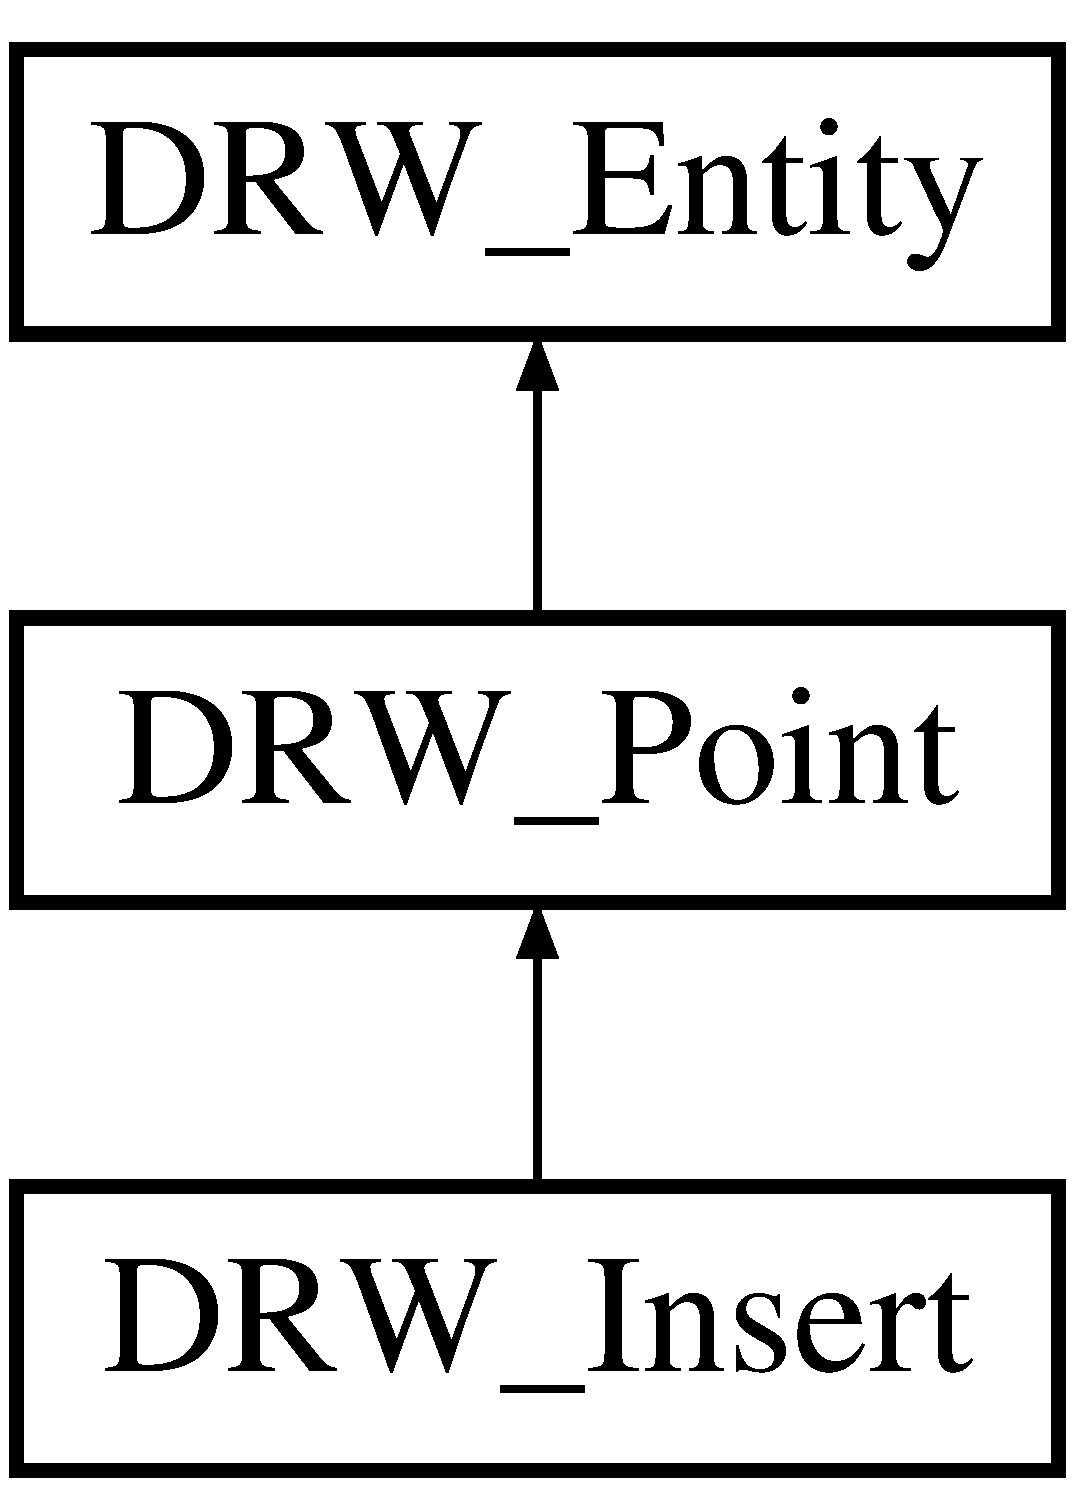
\includegraphics[height=3.000000cm]{df/d4f/class_d_r_w___insert}
\end{center}
\end{figure}
\subsection*{Public Attributes}
\begin{DoxyCompactItemize}
\item 
U\+T\+F8\+S\+T\+R\+I\+N\+G \hyperlink{class_d_r_w___insert_aac767b55f89a1ba2f95a01573dde4302}{name}
\item 
double \hyperlink{class_d_r_w___insert_a7b9b914c2570967914074f374ddbe9ef}{xscale}
\item 
double \hyperlink{class_d_r_w___insert_a412f380485be38075b05976337102a47}{yscale}
\item 
double \hyperlink{class_d_r_w___insert_a0f1cd0ef6b837894679b1135ce4bb132}{zscale}
\item 
double \hyperlink{class_d_r_w___insert_ad685a40847d4a5a8458ecaff2ccc4f3d}{angle}
\item 
int \hyperlink{class_d_r_w___insert_acd0f0491349b2159c6009634f883c3e7}{colcount}
\item 
int \hyperlink{class_d_r_w___insert_ac9bc5494805108fd83f5e1851d12b90b}{rowcount}
\item 
double \hyperlink{class_d_r_w___insert_a4fe4d62a16d3288286004aa8dd49acb6}{colspace}
\item 
double \hyperlink{class_d_r_w___insert_af9dde2e71b5fc348b0018c0e5c74d9cf}{rowspace}
\end{DoxyCompactItemize}
\subsection*{Additional Inherited Members}


\subsection{Detailed Description}
Class to handle insert entries. 

Class to handle insert entries \begin{DoxyAuthor}{Author}
Rallaz 
\end{DoxyAuthor}


\subsection{Member Data Documentation}
\hypertarget{class_d_r_w___insert_ad685a40847d4a5a8458ecaff2ccc4f3d}{}\index{D\+R\+W\+\_\+\+Insert@{D\+R\+W\+\_\+\+Insert}!angle@{angle}}
\index{angle@{angle}!D\+R\+W\+\_\+\+Insert@{D\+R\+W\+\_\+\+Insert}}
\subsubsection[{angle}]{\setlength{\rightskip}{0pt plus 5cm}double D\+R\+W\+\_\+\+Insert\+::angle}\label{class_d_r_w___insert_ad685a40847d4a5a8458ecaff2ccc4f3d}
rotation angle, code 50 \hypertarget{class_d_r_w___insert_acd0f0491349b2159c6009634f883c3e7}{}\index{D\+R\+W\+\_\+\+Insert@{D\+R\+W\+\_\+\+Insert}!colcount@{colcount}}
\index{colcount@{colcount}!D\+R\+W\+\_\+\+Insert@{D\+R\+W\+\_\+\+Insert}}
\subsubsection[{colcount}]{\setlength{\rightskip}{0pt plus 5cm}int D\+R\+W\+\_\+\+Insert\+::colcount}\label{class_d_r_w___insert_acd0f0491349b2159c6009634f883c3e7}
column count, code 70 \hypertarget{class_d_r_w___insert_a4fe4d62a16d3288286004aa8dd49acb6}{}\index{D\+R\+W\+\_\+\+Insert@{D\+R\+W\+\_\+\+Insert}!colspace@{colspace}}
\index{colspace@{colspace}!D\+R\+W\+\_\+\+Insert@{D\+R\+W\+\_\+\+Insert}}
\subsubsection[{colspace}]{\setlength{\rightskip}{0pt plus 5cm}double D\+R\+W\+\_\+\+Insert\+::colspace}\label{class_d_r_w___insert_a4fe4d62a16d3288286004aa8dd49acb6}
column space, code 44 \hypertarget{class_d_r_w___insert_aac767b55f89a1ba2f95a01573dde4302}{}\index{D\+R\+W\+\_\+\+Insert@{D\+R\+W\+\_\+\+Insert}!name@{name}}
\index{name@{name}!D\+R\+W\+\_\+\+Insert@{D\+R\+W\+\_\+\+Insert}}
\subsubsection[{name}]{\setlength{\rightskip}{0pt plus 5cm}U\+T\+F8\+S\+T\+R\+I\+N\+G D\+R\+W\+\_\+\+Insert\+::name}\label{class_d_r_w___insert_aac767b55f89a1ba2f95a01573dde4302}
block name, code 2 \hypertarget{class_d_r_w___insert_ac9bc5494805108fd83f5e1851d12b90b}{}\index{D\+R\+W\+\_\+\+Insert@{D\+R\+W\+\_\+\+Insert}!rowcount@{rowcount}}
\index{rowcount@{rowcount}!D\+R\+W\+\_\+\+Insert@{D\+R\+W\+\_\+\+Insert}}
\subsubsection[{rowcount}]{\setlength{\rightskip}{0pt plus 5cm}int D\+R\+W\+\_\+\+Insert\+::rowcount}\label{class_d_r_w___insert_ac9bc5494805108fd83f5e1851d12b90b}
row count, code 71 \hypertarget{class_d_r_w___insert_af9dde2e71b5fc348b0018c0e5c74d9cf}{}\index{D\+R\+W\+\_\+\+Insert@{D\+R\+W\+\_\+\+Insert}!rowspace@{rowspace}}
\index{rowspace@{rowspace}!D\+R\+W\+\_\+\+Insert@{D\+R\+W\+\_\+\+Insert}}
\subsubsection[{rowspace}]{\setlength{\rightskip}{0pt plus 5cm}double D\+R\+W\+\_\+\+Insert\+::rowspace}\label{class_d_r_w___insert_af9dde2e71b5fc348b0018c0e5c74d9cf}
row space, code 45 \hypertarget{class_d_r_w___insert_a7b9b914c2570967914074f374ddbe9ef}{}\index{D\+R\+W\+\_\+\+Insert@{D\+R\+W\+\_\+\+Insert}!xscale@{xscale}}
\index{xscale@{xscale}!D\+R\+W\+\_\+\+Insert@{D\+R\+W\+\_\+\+Insert}}
\subsubsection[{xscale}]{\setlength{\rightskip}{0pt plus 5cm}double D\+R\+W\+\_\+\+Insert\+::xscale}\label{class_d_r_w___insert_a7b9b914c2570967914074f374ddbe9ef}
x scale factor, code 41 \hypertarget{class_d_r_w___insert_a412f380485be38075b05976337102a47}{}\index{D\+R\+W\+\_\+\+Insert@{D\+R\+W\+\_\+\+Insert}!yscale@{yscale}}
\index{yscale@{yscale}!D\+R\+W\+\_\+\+Insert@{D\+R\+W\+\_\+\+Insert}}
\subsubsection[{yscale}]{\setlength{\rightskip}{0pt plus 5cm}double D\+R\+W\+\_\+\+Insert\+::yscale}\label{class_d_r_w___insert_a412f380485be38075b05976337102a47}
y scale factor, code 42 \hypertarget{class_d_r_w___insert_a0f1cd0ef6b837894679b1135ce4bb132}{}\index{D\+R\+W\+\_\+\+Insert@{D\+R\+W\+\_\+\+Insert}!zscale@{zscale}}
\index{zscale@{zscale}!D\+R\+W\+\_\+\+Insert@{D\+R\+W\+\_\+\+Insert}}
\subsubsection[{zscale}]{\setlength{\rightskip}{0pt plus 5cm}double D\+R\+W\+\_\+\+Insert\+::zscale}\label{class_d_r_w___insert_a0f1cd0ef6b837894679b1135ce4bb132}
z scale factor, code 43 

The documentation for this class was generated from the following files\+:\begin{DoxyCompactItemize}
\item 
src/drw\+\_\+entities.\+h\item 
src/drw\+\_\+entities.\+cpp\end{DoxyCompactItemize}

\hypertarget{class_d_r_w___interface}{}\section{D\+R\+W\+\_\+\+Interface Class Reference}
\label{class_d_r_w___interface}\index{D\+R\+W\+\_\+\+Interface@{D\+R\+W\+\_\+\+Interface}}


{\ttfamily \#include $<$drw\+\_\+interface.\+h$>$}

\subsection*{Public Member Functions}
\begin{DoxyCompactItemize}
\item 
virtual void \hyperlink{class_d_r_w___interface_a36ca28f76ddb6df58c683f29fc09e5db}{add\+Header} (const \hyperlink{class_d_r_w___header}{D\+R\+W\+\_\+\+Header} $\ast$data)=0
\item 
virtual void \hyperlink{class_d_r_w___interface_af0b179fdf1f4717b4ecf7570396ab17c}{add\+L\+Type} (const \hyperlink{class_d_r_w___l_type}{D\+R\+W\+\_\+\+L\+Type} \&data)=0
\item 
virtual void \hyperlink{class_d_r_w___interface_a14d5af0530b9d15c70e06695571f15a7}{add\+Layer} (const \hyperlink{class_d_r_w___layer}{D\+R\+W\+\_\+\+Layer} \&data)=0
\item 
virtual void \hyperlink{class_d_r_w___interface_ad9237d153a134b8e41a4e53b8e86dde5}{add\+Dim\+Style} (const \hyperlink{class_d_r_w___dimstyle}{D\+R\+W\+\_\+\+Dimstyle} \&data)=0
\item 
virtual void \hyperlink{class_d_r_w___interface_a62940fa7414131514a4eafcc7bb53af7}{add\+Vport} (const \hyperlink{class_d_r_w___vport}{D\+R\+W\+\_\+\+Vport} \&data)=0
\item 
virtual void \hyperlink{class_d_r_w___interface_a22da4ebff8bc7c1a426a27803a31b677}{add\+Text\+Style} (const \hyperlink{class_d_r_w___textstyle}{D\+R\+W\+\_\+\+Textstyle} \&data)=0
\item 
virtual void \hyperlink{class_d_r_w___interface_ac4e0727bb5223a4974052e20363b6f42}{add\+Block} (const \hyperlink{class_d_r_w___block}{D\+R\+W\+\_\+\+Block} \&data)=0
\item 
virtual void \hyperlink{class_d_r_w___interface_a31ea3946aa9e9042e7dc6d1cb37cf60b}{set\+Block} (const int handle)=0
\item 
virtual void \hyperlink{class_d_r_w___interface_aec16f6683828dbdb703b4b8db640d7a0}{end\+Block} ()=0
\item 
virtual void \hyperlink{class_d_r_w___interface_af1b9e163c87a3f84a5c06dbc2a6bd18b}{add\+Point} (const \hyperlink{class_d_r_w___point}{D\+R\+W\+\_\+\+Point} \&data)=0
\item 
virtual void \hyperlink{class_d_r_w___interface_a6422d075d59ed28408394bc5d68033e1}{add\+Line} (const \hyperlink{class_d_r_w___line}{D\+R\+W\+\_\+\+Line} \&data)=0
\item 
virtual void \hyperlink{class_d_r_w___interface_a4718019d01569f13a50a29fcb9ba583f}{add\+Ray} (const \hyperlink{class_d_r_w___ray}{D\+R\+W\+\_\+\+Ray} \&data)=0
\item 
virtual void \hyperlink{class_d_r_w___interface_a5cb4ece224c8006de498eb60e354ee9a}{add\+Xline} (const \hyperlink{class_d_r_w___xline}{D\+R\+W\+\_\+\+Xline} \&data)=0
\item 
virtual void \hyperlink{class_d_r_w___interface_a7abe9b6b69b8239fbad804eb68b0463e}{add\+Arc} (const \hyperlink{class_d_r_w___arc}{D\+R\+W\+\_\+\+Arc} \&data)=0
\item 
virtual void \hyperlink{class_d_r_w___interface_a921046eb1a06ad4753b9aaae9518af73}{add\+Circle} (const \hyperlink{class_d_r_w___circle}{D\+R\+W\+\_\+\+Circle} \&data)=0
\item 
virtual void \hyperlink{class_d_r_w___interface_a8a4d9d0ded98a7fa9ba5dd6d0005a491}{add\+Ellipse} (const \hyperlink{class_d_r_w___ellipse}{D\+R\+W\+\_\+\+Ellipse} \&data)=0
\item 
virtual void \hyperlink{class_d_r_w___interface_a14ec6d00f6f34857b91543497d9d4e09}{add\+L\+W\+Polyline} (const \hyperlink{class_d_r_w___l_w_polyline}{D\+R\+W\+\_\+\+L\+W\+Polyline} \&data)=0
\item 
virtual void \hyperlink{class_d_r_w___interface_a9e2c6ab12b71e73ab443765a5a42d171}{add\+Polyline} (const \hyperlink{class_d_r_w___polyline}{D\+R\+W\+\_\+\+Polyline} \&data)=0
\item 
virtual void \hyperlink{class_d_r_w___interface_a72d1cd0692fb061ea34ea246c54156ad}{add\+Spline} (const \hyperlink{class_d_r_w___spline}{D\+R\+W\+\_\+\+Spline} $\ast$data)=0
\item 
virtual void \hyperlink{class_d_r_w___interface_a6e19d01637ff9336bcd513511ba1177c}{add\+Knot} (const \hyperlink{class_d_r_w___entity}{D\+R\+W\+\_\+\+Entity} \&data)=0
\item 
virtual void \hyperlink{class_d_r_w___interface_a2aae96a5a0f5305d2e1f3254c871d2fc}{add\+Insert} (const \hyperlink{class_d_r_w___insert}{D\+R\+W\+\_\+\+Insert} \&data)=0
\item 
virtual void \hyperlink{class_d_r_w___interface_a3e09cf10863708e1ca74b2f723dc98a2}{add\+Trace} (const \hyperlink{class_d_r_w___trace}{D\+R\+W\+\_\+\+Trace} \&data)=0
\item 
virtual void \hyperlink{class_d_r_w___interface_a1664ed6d78dda11cf323776f594413fb}{add3d\+Face} (const \hyperlink{class_d_r_w__3_dface}{D\+R\+W\+\_\+3\+Dface} \&data)=0
\item 
virtual void \hyperlink{class_d_r_w___interface_a1d50d3aae16fb70d997b82f1bf2cbb4f}{add\+Solid} (const \hyperlink{class_d_r_w___solid}{D\+R\+W\+\_\+\+Solid} \&data)=0
\item 
virtual void \hyperlink{class_d_r_w___interface_a2a9e71a0794a3f8f5191bd9bc9e51bad}{add\+M\+Text} (const \hyperlink{class_d_r_w___m_text}{D\+R\+W\+\_\+\+M\+Text} \&data)=0
\item 
virtual void \hyperlink{class_d_r_w___interface_a13be257d7e54629f3173fad53448c0a7}{add\+Text} (const \hyperlink{class_d_r_w___text}{D\+R\+W\+\_\+\+Text} \&data)=0
\item 
virtual void \hyperlink{class_d_r_w___interface_a6f351237a9d4f10c3f9651c68966a3fb}{add\+Dim\+Align} (const \hyperlink{class_d_r_w___dim_aligned}{D\+R\+W\+\_\+\+Dim\+Aligned} $\ast$data)=0
\item 
virtual void \hyperlink{class_d_r_w___interface_a81d63111186b65e662fd0fecfa09da2e}{add\+Dim\+Linear} (const \hyperlink{class_d_r_w___dim_linear}{D\+R\+W\+\_\+\+Dim\+Linear} $\ast$data)=0
\item 
virtual void \hyperlink{class_d_r_w___interface_a50307476a7aa8065ee5462cd7fdce3c6}{add\+Dim\+Radial} (const \hyperlink{class_d_r_w___dim_radial}{D\+R\+W\+\_\+\+Dim\+Radial} $\ast$data)=0
\item 
virtual void \hyperlink{class_d_r_w___interface_a63948977f0a34dd29697f0db7e24a6ed}{add\+Dim\+Diametric} (const \hyperlink{class_d_r_w___dim_diametric}{D\+R\+W\+\_\+\+Dim\+Diametric} $\ast$data)=0
\item 
virtual void \hyperlink{class_d_r_w___interface_af53ce2878a9327464897aa1cb8e7a333}{add\+Dim\+Angular} (const \hyperlink{class_d_r_w___dim_angular}{D\+R\+W\+\_\+\+Dim\+Angular} $\ast$data)=0
\item 
virtual void \hyperlink{class_d_r_w___interface_abdeea17ef54bd623e569f492943f1e9d}{add\+Dim\+Angular3\+P} (const \hyperlink{class_d_r_w___dim_angular3p}{D\+R\+W\+\_\+\+Dim\+Angular3p} $\ast$data)=0
\item 
virtual void \hyperlink{class_d_r_w___interface_ab3e89843322248d2a0e87dedb9cb9aec}{add\+Dim\+Ordinate} (const \hyperlink{class_d_r_w___dim_ordinate}{D\+R\+W\+\_\+\+Dim\+Ordinate} $\ast$data)=0
\item 
virtual void \hyperlink{class_d_r_w___interface_a10b2f081689b5a89e3cced928e60369a}{add\+Leader} (const \hyperlink{class_d_r_w___leader}{D\+R\+W\+\_\+\+Leader} $\ast$data)=0
\item 
virtual void \hyperlink{class_d_r_w___interface_a486e160f61c3e86e53bb8b801b9bbbab}{add\+Hatch} (const \hyperlink{class_d_r_w___hatch}{D\+R\+W\+\_\+\+Hatch} $\ast$data)=0
\item 
virtual void \hyperlink{class_d_r_w___interface_a6127b0330b671d2cb1be73478ff24945}{add\+Viewport} (const \hyperlink{class_d_r_w___viewport}{D\+R\+W\+\_\+\+Viewport} \&data)=0
\item 
virtual void \hyperlink{class_d_r_w___interface_a90f17ffeb31d7b41c0ff23eb396c60e2}{add\+Image} (const \hyperlink{class_d_r_w___image}{D\+R\+W\+\_\+\+Image} $\ast$data)=0
\item 
virtual void \hyperlink{class_d_r_w___interface_a8f7969f1639e6544e82446bc21e71446}{link\+Image} (const \hyperlink{class_d_r_w___image_def}{D\+R\+W\+\_\+\+Image\+Def} $\ast$data)=0
\item 
virtual void \hyperlink{class_d_r_w___interface_a4b9bb278a16a1ceaa53ebe05dab93b42}{add\+Comment} (const char $\ast$comment)=0
\end{DoxyCompactItemize}


\subsection{Detailed Description}
Abstract class (interface) for comunicate dxf\+Reader with the application. Inherit your class which takes care of the entities in the processed D\+X\+F file from this interface.

\begin{DoxyAuthor}{Author}
Rallaz 
\end{DoxyAuthor}


\subsection{Member Function Documentation}
\hypertarget{class_d_r_w___interface_a1664ed6d78dda11cf323776f594413fb}{}\index{D\+R\+W\+\_\+\+Interface@{D\+R\+W\+\_\+\+Interface}!add3d\+Face@{add3d\+Face}}
\index{add3d\+Face@{add3d\+Face}!D\+R\+W\+\_\+\+Interface@{D\+R\+W\+\_\+\+Interface}}
\subsubsection[{add3d\+Face}]{\setlength{\rightskip}{0pt plus 5cm}virtual void D\+R\+W\+\_\+\+Interface\+::add3d\+Face (
\begin{DoxyParamCaption}
\item[{const {\bf D\+R\+W\+\_\+3\+Dface} \&}]{data}
\end{DoxyParamCaption}
)\hspace{0.3cm}{\ttfamily [pure virtual]}}\label{class_d_r_w___interface_a1664ed6d78dda11cf323776f594413fb}
Called for every 3dface start \hypertarget{class_d_r_w___interface_a7abe9b6b69b8239fbad804eb68b0463e}{}\index{D\+R\+W\+\_\+\+Interface@{D\+R\+W\+\_\+\+Interface}!add\+Arc@{add\+Arc}}
\index{add\+Arc@{add\+Arc}!D\+R\+W\+\_\+\+Interface@{D\+R\+W\+\_\+\+Interface}}
\subsubsection[{add\+Arc}]{\setlength{\rightskip}{0pt plus 5cm}virtual void D\+R\+W\+\_\+\+Interface\+::add\+Arc (
\begin{DoxyParamCaption}
\item[{const {\bf D\+R\+W\+\_\+\+Arc} \&}]{data}
\end{DoxyParamCaption}
)\hspace{0.3cm}{\ttfamily [pure virtual]}}\label{class_d_r_w___interface_a7abe9b6b69b8239fbad804eb68b0463e}
Called for every arc \hypertarget{class_d_r_w___interface_ac4e0727bb5223a4974052e20363b6f42}{}\index{D\+R\+W\+\_\+\+Interface@{D\+R\+W\+\_\+\+Interface}!add\+Block@{add\+Block}}
\index{add\+Block@{add\+Block}!D\+R\+W\+\_\+\+Interface@{D\+R\+W\+\_\+\+Interface}}
\subsubsection[{add\+Block}]{\setlength{\rightskip}{0pt plus 5cm}virtual void D\+R\+W\+\_\+\+Interface\+::add\+Block (
\begin{DoxyParamCaption}
\item[{const {\bf D\+R\+W\+\_\+\+Block} \&}]{data}
\end{DoxyParamCaption}
)\hspace{0.3cm}{\ttfamily [pure virtual]}}\label{class_d_r_w___interface_ac4e0727bb5223a4974052e20363b6f42}
Called for every block. Note\+: all entities added after this command go into this block until \hyperlink{class_d_r_w___interface_aec16f6683828dbdb703b4b8db640d7a0}{end\+Block()} is called.

\begin{DoxySeeAlso}{See also}
\hyperlink{class_d_r_w___interface_aec16f6683828dbdb703b4b8db640d7a0}{end\+Block()} 
\end{DoxySeeAlso}
\hypertarget{class_d_r_w___interface_a921046eb1a06ad4753b9aaae9518af73}{}\index{D\+R\+W\+\_\+\+Interface@{D\+R\+W\+\_\+\+Interface}!add\+Circle@{add\+Circle}}
\index{add\+Circle@{add\+Circle}!D\+R\+W\+\_\+\+Interface@{D\+R\+W\+\_\+\+Interface}}
\subsubsection[{add\+Circle}]{\setlength{\rightskip}{0pt plus 5cm}virtual void D\+R\+W\+\_\+\+Interface\+::add\+Circle (
\begin{DoxyParamCaption}
\item[{const {\bf D\+R\+W\+\_\+\+Circle} \&}]{data}
\end{DoxyParamCaption}
)\hspace{0.3cm}{\ttfamily [pure virtual]}}\label{class_d_r_w___interface_a921046eb1a06ad4753b9aaae9518af73}
Called for every circle \hypertarget{class_d_r_w___interface_a4b9bb278a16a1ceaa53ebe05dab93b42}{}\index{D\+R\+W\+\_\+\+Interface@{D\+R\+W\+\_\+\+Interface}!add\+Comment@{add\+Comment}}
\index{add\+Comment@{add\+Comment}!D\+R\+W\+\_\+\+Interface@{D\+R\+W\+\_\+\+Interface}}
\subsubsection[{add\+Comment}]{\setlength{\rightskip}{0pt plus 5cm}virtual void D\+R\+W\+\_\+\+Interface\+::add\+Comment (
\begin{DoxyParamCaption}
\item[{const char $\ast$}]{comment}
\end{DoxyParamCaption}
)\hspace{0.3cm}{\ttfamily [pure virtual]}}\label{class_d_r_w___interface_a4b9bb278a16a1ceaa53ebe05dab93b42}
Called for every comment in the D\+X\+F file (code 999). \hypertarget{class_d_r_w___interface_a6f351237a9d4f10c3f9651c68966a3fb}{}\index{D\+R\+W\+\_\+\+Interface@{D\+R\+W\+\_\+\+Interface}!add\+Dim\+Align@{add\+Dim\+Align}}
\index{add\+Dim\+Align@{add\+Dim\+Align}!D\+R\+W\+\_\+\+Interface@{D\+R\+W\+\_\+\+Interface}}
\subsubsection[{add\+Dim\+Align}]{\setlength{\rightskip}{0pt plus 5cm}virtual void D\+R\+W\+\_\+\+Interface\+::add\+Dim\+Align (
\begin{DoxyParamCaption}
\item[{const {\bf D\+R\+W\+\_\+\+Dim\+Aligned} $\ast$}]{data}
\end{DoxyParamCaption}
)\hspace{0.3cm}{\ttfamily [pure virtual]}}\label{class_d_r_w___interface_a6f351237a9d4f10c3f9651c68966a3fb}
Called for every aligned dimension entity. \hypertarget{class_d_r_w___interface_af53ce2878a9327464897aa1cb8e7a333}{}\index{D\+R\+W\+\_\+\+Interface@{D\+R\+W\+\_\+\+Interface}!add\+Dim\+Angular@{add\+Dim\+Angular}}
\index{add\+Dim\+Angular@{add\+Dim\+Angular}!D\+R\+W\+\_\+\+Interface@{D\+R\+W\+\_\+\+Interface}}
\subsubsection[{add\+Dim\+Angular}]{\setlength{\rightskip}{0pt plus 5cm}virtual void D\+R\+W\+\_\+\+Interface\+::add\+Dim\+Angular (
\begin{DoxyParamCaption}
\item[{const {\bf D\+R\+W\+\_\+\+Dim\+Angular} $\ast$}]{data}
\end{DoxyParamCaption}
)\hspace{0.3cm}{\ttfamily [pure virtual]}}\label{class_d_r_w___interface_af53ce2878a9327464897aa1cb8e7a333}
Called for every angular dimension (2 lines version) entity. \hypertarget{class_d_r_w___interface_abdeea17ef54bd623e569f492943f1e9d}{}\index{D\+R\+W\+\_\+\+Interface@{D\+R\+W\+\_\+\+Interface}!add\+Dim\+Angular3\+P@{add\+Dim\+Angular3\+P}}
\index{add\+Dim\+Angular3\+P@{add\+Dim\+Angular3\+P}!D\+R\+W\+\_\+\+Interface@{D\+R\+W\+\_\+\+Interface}}
\subsubsection[{add\+Dim\+Angular3\+P}]{\setlength{\rightskip}{0pt plus 5cm}virtual void D\+R\+W\+\_\+\+Interface\+::add\+Dim\+Angular3\+P (
\begin{DoxyParamCaption}
\item[{const {\bf D\+R\+W\+\_\+\+Dim\+Angular3p} $\ast$}]{data}
\end{DoxyParamCaption}
)\hspace{0.3cm}{\ttfamily [pure virtual]}}\label{class_d_r_w___interface_abdeea17ef54bd623e569f492943f1e9d}
Called for every angular dimension (3 points version) entity. \hypertarget{class_d_r_w___interface_a63948977f0a34dd29697f0db7e24a6ed}{}\index{D\+R\+W\+\_\+\+Interface@{D\+R\+W\+\_\+\+Interface}!add\+Dim\+Diametric@{add\+Dim\+Diametric}}
\index{add\+Dim\+Diametric@{add\+Dim\+Diametric}!D\+R\+W\+\_\+\+Interface@{D\+R\+W\+\_\+\+Interface}}
\subsubsection[{add\+Dim\+Diametric}]{\setlength{\rightskip}{0pt plus 5cm}virtual void D\+R\+W\+\_\+\+Interface\+::add\+Dim\+Diametric (
\begin{DoxyParamCaption}
\item[{const {\bf D\+R\+W\+\_\+\+Dim\+Diametric} $\ast$}]{data}
\end{DoxyParamCaption}
)\hspace{0.3cm}{\ttfamily [pure virtual]}}\label{class_d_r_w___interface_a63948977f0a34dd29697f0db7e24a6ed}
Called for every diametric dimension entity. \hypertarget{class_d_r_w___interface_a81d63111186b65e662fd0fecfa09da2e}{}\index{D\+R\+W\+\_\+\+Interface@{D\+R\+W\+\_\+\+Interface}!add\+Dim\+Linear@{add\+Dim\+Linear}}
\index{add\+Dim\+Linear@{add\+Dim\+Linear}!D\+R\+W\+\_\+\+Interface@{D\+R\+W\+\_\+\+Interface}}
\subsubsection[{add\+Dim\+Linear}]{\setlength{\rightskip}{0pt plus 5cm}virtual void D\+R\+W\+\_\+\+Interface\+::add\+Dim\+Linear (
\begin{DoxyParamCaption}
\item[{const {\bf D\+R\+W\+\_\+\+Dim\+Linear} $\ast$}]{data}
\end{DoxyParamCaption}
)\hspace{0.3cm}{\ttfamily [pure virtual]}}\label{class_d_r_w___interface_a81d63111186b65e662fd0fecfa09da2e}
Called for every linear or rotated dimension entity. \hypertarget{class_d_r_w___interface_ab3e89843322248d2a0e87dedb9cb9aec}{}\index{D\+R\+W\+\_\+\+Interface@{D\+R\+W\+\_\+\+Interface}!add\+Dim\+Ordinate@{add\+Dim\+Ordinate}}
\index{add\+Dim\+Ordinate@{add\+Dim\+Ordinate}!D\+R\+W\+\_\+\+Interface@{D\+R\+W\+\_\+\+Interface}}
\subsubsection[{add\+Dim\+Ordinate}]{\setlength{\rightskip}{0pt plus 5cm}virtual void D\+R\+W\+\_\+\+Interface\+::add\+Dim\+Ordinate (
\begin{DoxyParamCaption}
\item[{const {\bf D\+R\+W\+\_\+\+Dim\+Ordinate} $\ast$}]{data}
\end{DoxyParamCaption}
)\hspace{0.3cm}{\ttfamily [pure virtual]}}\label{class_d_r_w___interface_ab3e89843322248d2a0e87dedb9cb9aec}
Called for every ordinate dimension entity. \hypertarget{class_d_r_w___interface_a50307476a7aa8065ee5462cd7fdce3c6}{}\index{D\+R\+W\+\_\+\+Interface@{D\+R\+W\+\_\+\+Interface}!add\+Dim\+Radial@{add\+Dim\+Radial}}
\index{add\+Dim\+Radial@{add\+Dim\+Radial}!D\+R\+W\+\_\+\+Interface@{D\+R\+W\+\_\+\+Interface}}
\subsubsection[{add\+Dim\+Radial}]{\setlength{\rightskip}{0pt plus 5cm}virtual void D\+R\+W\+\_\+\+Interface\+::add\+Dim\+Radial (
\begin{DoxyParamCaption}
\item[{const {\bf D\+R\+W\+\_\+\+Dim\+Radial} $\ast$}]{data}
\end{DoxyParamCaption}
)\hspace{0.3cm}{\ttfamily [pure virtual]}}\label{class_d_r_w___interface_a50307476a7aa8065ee5462cd7fdce3c6}
Called for every radial dimension entity. \hypertarget{class_d_r_w___interface_ad9237d153a134b8e41a4e53b8e86dde5}{}\index{D\+R\+W\+\_\+\+Interface@{D\+R\+W\+\_\+\+Interface}!add\+Dim\+Style@{add\+Dim\+Style}}
\index{add\+Dim\+Style@{add\+Dim\+Style}!D\+R\+W\+\_\+\+Interface@{D\+R\+W\+\_\+\+Interface}}
\subsubsection[{add\+Dim\+Style}]{\setlength{\rightskip}{0pt plus 5cm}virtual void D\+R\+W\+\_\+\+Interface\+::add\+Dim\+Style (
\begin{DoxyParamCaption}
\item[{const {\bf D\+R\+W\+\_\+\+Dimstyle} \&}]{data}
\end{DoxyParamCaption}
)\hspace{0.3cm}{\ttfamily [pure virtual]}}\label{class_d_r_w___interface_ad9237d153a134b8e41a4e53b8e86dde5}
Called for every dim style. \hypertarget{class_d_r_w___interface_a8a4d9d0ded98a7fa9ba5dd6d0005a491}{}\index{D\+R\+W\+\_\+\+Interface@{D\+R\+W\+\_\+\+Interface}!add\+Ellipse@{add\+Ellipse}}
\index{add\+Ellipse@{add\+Ellipse}!D\+R\+W\+\_\+\+Interface@{D\+R\+W\+\_\+\+Interface}}
\subsubsection[{add\+Ellipse}]{\setlength{\rightskip}{0pt plus 5cm}virtual void D\+R\+W\+\_\+\+Interface\+::add\+Ellipse (
\begin{DoxyParamCaption}
\item[{const {\bf D\+R\+W\+\_\+\+Ellipse} \&}]{data}
\end{DoxyParamCaption}
)\hspace{0.3cm}{\ttfamily [pure virtual]}}\label{class_d_r_w___interface_a8a4d9d0ded98a7fa9ba5dd6d0005a491}
Called for every ellipse \hypertarget{class_d_r_w___interface_a486e160f61c3e86e53bb8b801b9bbbab}{}\index{D\+R\+W\+\_\+\+Interface@{D\+R\+W\+\_\+\+Interface}!add\+Hatch@{add\+Hatch}}
\index{add\+Hatch@{add\+Hatch}!D\+R\+W\+\_\+\+Interface@{D\+R\+W\+\_\+\+Interface}}
\subsubsection[{add\+Hatch}]{\setlength{\rightskip}{0pt plus 5cm}virtual void D\+R\+W\+\_\+\+Interface\+::add\+Hatch (
\begin{DoxyParamCaption}
\item[{const {\bf D\+R\+W\+\_\+\+Hatch} $\ast$}]{data}
\end{DoxyParamCaption}
)\hspace{0.3cm}{\ttfamily [pure virtual]}}\label{class_d_r_w___interface_a486e160f61c3e86e53bb8b801b9bbbab}
Called for every hatch entity. \hypertarget{class_d_r_w___interface_a36ca28f76ddb6df58c683f29fc09e5db}{}\index{D\+R\+W\+\_\+\+Interface@{D\+R\+W\+\_\+\+Interface}!add\+Header@{add\+Header}}
\index{add\+Header@{add\+Header}!D\+R\+W\+\_\+\+Interface@{D\+R\+W\+\_\+\+Interface}}
\subsubsection[{add\+Header}]{\setlength{\rightskip}{0pt plus 5cm}virtual void D\+R\+W\+\_\+\+Interface\+::add\+Header (
\begin{DoxyParamCaption}
\item[{const {\bf D\+R\+W\+\_\+\+Header} $\ast$}]{data}
\end{DoxyParamCaption}
)\hspace{0.3cm}{\ttfamily [pure virtual]}}\label{class_d_r_w___interface_a36ca28f76ddb6df58c683f29fc09e5db}
Called when header is parsed. \hypertarget{class_d_r_w___interface_a90f17ffeb31d7b41c0ff23eb396c60e2}{}\index{D\+R\+W\+\_\+\+Interface@{D\+R\+W\+\_\+\+Interface}!add\+Image@{add\+Image}}
\index{add\+Image@{add\+Image}!D\+R\+W\+\_\+\+Interface@{D\+R\+W\+\_\+\+Interface}}
\subsubsection[{add\+Image}]{\setlength{\rightskip}{0pt plus 5cm}virtual void D\+R\+W\+\_\+\+Interface\+::add\+Image (
\begin{DoxyParamCaption}
\item[{const {\bf D\+R\+W\+\_\+\+Image} $\ast$}]{data}
\end{DoxyParamCaption}
)\hspace{0.3cm}{\ttfamily [pure virtual]}}\label{class_d_r_w___interface_a90f17ffeb31d7b41c0ff23eb396c60e2}
Called for every image entity. \hypertarget{class_d_r_w___interface_a2aae96a5a0f5305d2e1f3254c871d2fc}{}\index{D\+R\+W\+\_\+\+Interface@{D\+R\+W\+\_\+\+Interface}!add\+Insert@{add\+Insert}}
\index{add\+Insert@{add\+Insert}!D\+R\+W\+\_\+\+Interface@{D\+R\+W\+\_\+\+Interface}}
\subsubsection[{add\+Insert}]{\setlength{\rightskip}{0pt plus 5cm}virtual void D\+R\+W\+\_\+\+Interface\+::add\+Insert (
\begin{DoxyParamCaption}
\item[{const {\bf D\+R\+W\+\_\+\+Insert} \&}]{data}
\end{DoxyParamCaption}
)\hspace{0.3cm}{\ttfamily [pure virtual]}}\label{class_d_r_w___interface_a2aae96a5a0f5305d2e1f3254c871d2fc}
Called for every insert. \hypertarget{class_d_r_w___interface_a6e19d01637ff9336bcd513511ba1177c}{}\index{D\+R\+W\+\_\+\+Interface@{D\+R\+W\+\_\+\+Interface}!add\+Knot@{add\+Knot}}
\index{add\+Knot@{add\+Knot}!D\+R\+W\+\_\+\+Interface@{D\+R\+W\+\_\+\+Interface}}
\subsubsection[{add\+Knot}]{\setlength{\rightskip}{0pt plus 5cm}virtual void D\+R\+W\+\_\+\+Interface\+::add\+Knot (
\begin{DoxyParamCaption}
\item[{const {\bf D\+R\+W\+\_\+\+Entity} \&}]{data}
\end{DoxyParamCaption}
)\hspace{0.3cm}{\ttfamily [pure virtual]}}\label{class_d_r_w___interface_a6e19d01637ff9336bcd513511ba1177c}
Called for every spline knot value \hypertarget{class_d_r_w___interface_a14d5af0530b9d15c70e06695571f15a7}{}\index{D\+R\+W\+\_\+\+Interface@{D\+R\+W\+\_\+\+Interface}!add\+Layer@{add\+Layer}}
\index{add\+Layer@{add\+Layer}!D\+R\+W\+\_\+\+Interface@{D\+R\+W\+\_\+\+Interface}}
\subsubsection[{add\+Layer}]{\setlength{\rightskip}{0pt plus 5cm}virtual void D\+R\+W\+\_\+\+Interface\+::add\+Layer (
\begin{DoxyParamCaption}
\item[{const {\bf D\+R\+W\+\_\+\+Layer} \&}]{data}
\end{DoxyParamCaption}
)\hspace{0.3cm}{\ttfamily [pure virtual]}}\label{class_d_r_w___interface_a14d5af0530b9d15c70e06695571f15a7}
Called for every layer. \hypertarget{class_d_r_w___interface_a10b2f081689b5a89e3cced928e60369a}{}\index{D\+R\+W\+\_\+\+Interface@{D\+R\+W\+\_\+\+Interface}!add\+Leader@{add\+Leader}}
\index{add\+Leader@{add\+Leader}!D\+R\+W\+\_\+\+Interface@{D\+R\+W\+\_\+\+Interface}}
\subsubsection[{add\+Leader}]{\setlength{\rightskip}{0pt plus 5cm}virtual void D\+R\+W\+\_\+\+Interface\+::add\+Leader (
\begin{DoxyParamCaption}
\item[{const {\bf D\+R\+W\+\_\+\+Leader} $\ast$}]{data}
\end{DoxyParamCaption}
)\hspace{0.3cm}{\ttfamily [pure virtual]}}\label{class_d_r_w___interface_a10b2f081689b5a89e3cced928e60369a}
Called for every leader start. \hypertarget{class_d_r_w___interface_a6422d075d59ed28408394bc5d68033e1}{}\index{D\+R\+W\+\_\+\+Interface@{D\+R\+W\+\_\+\+Interface}!add\+Line@{add\+Line}}
\index{add\+Line@{add\+Line}!D\+R\+W\+\_\+\+Interface@{D\+R\+W\+\_\+\+Interface}}
\subsubsection[{add\+Line}]{\setlength{\rightskip}{0pt plus 5cm}virtual void D\+R\+W\+\_\+\+Interface\+::add\+Line (
\begin{DoxyParamCaption}
\item[{const {\bf D\+R\+W\+\_\+\+Line} \&}]{data}
\end{DoxyParamCaption}
)\hspace{0.3cm}{\ttfamily [pure virtual]}}\label{class_d_r_w___interface_a6422d075d59ed28408394bc5d68033e1}
Called for every line \hypertarget{class_d_r_w___interface_af0b179fdf1f4717b4ecf7570396ab17c}{}\index{D\+R\+W\+\_\+\+Interface@{D\+R\+W\+\_\+\+Interface}!add\+L\+Type@{add\+L\+Type}}
\index{add\+L\+Type@{add\+L\+Type}!D\+R\+W\+\_\+\+Interface@{D\+R\+W\+\_\+\+Interface}}
\subsubsection[{add\+L\+Type}]{\setlength{\rightskip}{0pt plus 5cm}virtual void D\+R\+W\+\_\+\+Interface\+::add\+L\+Type (
\begin{DoxyParamCaption}
\item[{const {\bf D\+R\+W\+\_\+\+L\+Type} \&}]{data}
\end{DoxyParamCaption}
)\hspace{0.3cm}{\ttfamily [pure virtual]}}\label{class_d_r_w___interface_af0b179fdf1f4717b4ecf7570396ab17c}
Called for every line Type. \hypertarget{class_d_r_w___interface_a14ec6d00f6f34857b91543497d9d4e09}{}\index{D\+R\+W\+\_\+\+Interface@{D\+R\+W\+\_\+\+Interface}!add\+L\+W\+Polyline@{add\+L\+W\+Polyline}}
\index{add\+L\+W\+Polyline@{add\+L\+W\+Polyline}!D\+R\+W\+\_\+\+Interface@{D\+R\+W\+\_\+\+Interface}}
\subsubsection[{add\+L\+W\+Polyline}]{\setlength{\rightskip}{0pt plus 5cm}virtual void D\+R\+W\+\_\+\+Interface\+::add\+L\+W\+Polyline (
\begin{DoxyParamCaption}
\item[{const {\bf D\+R\+W\+\_\+\+L\+W\+Polyline} \&}]{data}
\end{DoxyParamCaption}
)\hspace{0.3cm}{\ttfamily [pure virtual]}}\label{class_d_r_w___interface_a14ec6d00f6f34857b91543497d9d4e09}
Called for every lwpolyline \hypertarget{class_d_r_w___interface_a2a9e71a0794a3f8f5191bd9bc9e51bad}{}\index{D\+R\+W\+\_\+\+Interface@{D\+R\+W\+\_\+\+Interface}!add\+M\+Text@{add\+M\+Text}}
\index{add\+M\+Text@{add\+M\+Text}!D\+R\+W\+\_\+\+Interface@{D\+R\+W\+\_\+\+Interface}}
\subsubsection[{add\+M\+Text}]{\setlength{\rightskip}{0pt plus 5cm}virtual void D\+R\+W\+\_\+\+Interface\+::add\+M\+Text (
\begin{DoxyParamCaption}
\item[{const {\bf D\+R\+W\+\_\+\+M\+Text} \&}]{data}
\end{DoxyParamCaption}
)\hspace{0.3cm}{\ttfamily [pure virtual]}}\label{class_d_r_w___interface_a2a9e71a0794a3f8f5191bd9bc9e51bad}
Called for every Multi Text entity. \hypertarget{class_d_r_w___interface_af1b9e163c87a3f84a5c06dbc2a6bd18b}{}\index{D\+R\+W\+\_\+\+Interface@{D\+R\+W\+\_\+\+Interface}!add\+Point@{add\+Point}}
\index{add\+Point@{add\+Point}!D\+R\+W\+\_\+\+Interface@{D\+R\+W\+\_\+\+Interface}}
\subsubsection[{add\+Point}]{\setlength{\rightskip}{0pt plus 5cm}virtual void D\+R\+W\+\_\+\+Interface\+::add\+Point (
\begin{DoxyParamCaption}
\item[{const {\bf D\+R\+W\+\_\+\+Point} \&}]{data}
\end{DoxyParamCaption}
)\hspace{0.3cm}{\ttfamily [pure virtual]}}\label{class_d_r_w___interface_af1b9e163c87a3f84a5c06dbc2a6bd18b}
Called for every point \hypertarget{class_d_r_w___interface_a9e2c6ab12b71e73ab443765a5a42d171}{}\index{D\+R\+W\+\_\+\+Interface@{D\+R\+W\+\_\+\+Interface}!add\+Polyline@{add\+Polyline}}
\index{add\+Polyline@{add\+Polyline}!D\+R\+W\+\_\+\+Interface@{D\+R\+W\+\_\+\+Interface}}
\subsubsection[{add\+Polyline}]{\setlength{\rightskip}{0pt plus 5cm}virtual void D\+R\+W\+\_\+\+Interface\+::add\+Polyline (
\begin{DoxyParamCaption}
\item[{const {\bf D\+R\+W\+\_\+\+Polyline} \&}]{data}
\end{DoxyParamCaption}
)\hspace{0.3cm}{\ttfamily [pure virtual]}}\label{class_d_r_w___interface_a9e2c6ab12b71e73ab443765a5a42d171}
Called for every polyline start \hypertarget{class_d_r_w___interface_a4718019d01569f13a50a29fcb9ba583f}{}\index{D\+R\+W\+\_\+\+Interface@{D\+R\+W\+\_\+\+Interface}!add\+Ray@{add\+Ray}}
\index{add\+Ray@{add\+Ray}!D\+R\+W\+\_\+\+Interface@{D\+R\+W\+\_\+\+Interface}}
\subsubsection[{add\+Ray}]{\setlength{\rightskip}{0pt plus 5cm}virtual void D\+R\+W\+\_\+\+Interface\+::add\+Ray (
\begin{DoxyParamCaption}
\item[{const {\bf D\+R\+W\+\_\+\+Ray} \&}]{data}
\end{DoxyParamCaption}
)\hspace{0.3cm}{\ttfamily [pure virtual]}}\label{class_d_r_w___interface_a4718019d01569f13a50a29fcb9ba583f}
Called for every ray \hypertarget{class_d_r_w___interface_a1d50d3aae16fb70d997b82f1bf2cbb4f}{}\index{D\+R\+W\+\_\+\+Interface@{D\+R\+W\+\_\+\+Interface}!add\+Solid@{add\+Solid}}
\index{add\+Solid@{add\+Solid}!D\+R\+W\+\_\+\+Interface@{D\+R\+W\+\_\+\+Interface}}
\subsubsection[{add\+Solid}]{\setlength{\rightskip}{0pt plus 5cm}virtual void D\+R\+W\+\_\+\+Interface\+::add\+Solid (
\begin{DoxyParamCaption}
\item[{const {\bf D\+R\+W\+\_\+\+Solid} \&}]{data}
\end{DoxyParamCaption}
)\hspace{0.3cm}{\ttfamily [pure virtual]}}\label{class_d_r_w___interface_a1d50d3aae16fb70d997b82f1bf2cbb4f}
Called for every solid start \hypertarget{class_d_r_w___interface_a72d1cd0692fb061ea34ea246c54156ad}{}\index{D\+R\+W\+\_\+\+Interface@{D\+R\+W\+\_\+\+Interface}!add\+Spline@{add\+Spline}}
\index{add\+Spline@{add\+Spline}!D\+R\+W\+\_\+\+Interface@{D\+R\+W\+\_\+\+Interface}}
\subsubsection[{add\+Spline}]{\setlength{\rightskip}{0pt plus 5cm}virtual void D\+R\+W\+\_\+\+Interface\+::add\+Spline (
\begin{DoxyParamCaption}
\item[{const {\bf D\+R\+W\+\_\+\+Spline} $\ast$}]{data}
\end{DoxyParamCaption}
)\hspace{0.3cm}{\ttfamily [pure virtual]}}\label{class_d_r_w___interface_a72d1cd0692fb061ea34ea246c54156ad}
Called for every spline \hypertarget{class_d_r_w___interface_a13be257d7e54629f3173fad53448c0a7}{}\index{D\+R\+W\+\_\+\+Interface@{D\+R\+W\+\_\+\+Interface}!add\+Text@{add\+Text}}
\index{add\+Text@{add\+Text}!D\+R\+W\+\_\+\+Interface@{D\+R\+W\+\_\+\+Interface}}
\subsubsection[{add\+Text}]{\setlength{\rightskip}{0pt plus 5cm}virtual void D\+R\+W\+\_\+\+Interface\+::add\+Text (
\begin{DoxyParamCaption}
\item[{const {\bf D\+R\+W\+\_\+\+Text} \&}]{data}
\end{DoxyParamCaption}
)\hspace{0.3cm}{\ttfamily [pure virtual]}}\label{class_d_r_w___interface_a13be257d7e54629f3173fad53448c0a7}
Called for every Text entity. \hypertarget{class_d_r_w___interface_a22da4ebff8bc7c1a426a27803a31b677}{}\index{D\+R\+W\+\_\+\+Interface@{D\+R\+W\+\_\+\+Interface}!add\+Text\+Style@{add\+Text\+Style}}
\index{add\+Text\+Style@{add\+Text\+Style}!D\+R\+W\+\_\+\+Interface@{D\+R\+W\+\_\+\+Interface}}
\subsubsection[{add\+Text\+Style}]{\setlength{\rightskip}{0pt plus 5cm}virtual void D\+R\+W\+\_\+\+Interface\+::add\+Text\+Style (
\begin{DoxyParamCaption}
\item[{const {\bf D\+R\+W\+\_\+\+Textstyle} \&}]{data}
\end{DoxyParamCaption}
)\hspace{0.3cm}{\ttfamily [pure virtual]}}\label{class_d_r_w___interface_a22da4ebff8bc7c1a426a27803a31b677}
Called for every text style. \hypertarget{class_d_r_w___interface_a3e09cf10863708e1ca74b2f723dc98a2}{}\index{D\+R\+W\+\_\+\+Interface@{D\+R\+W\+\_\+\+Interface}!add\+Trace@{add\+Trace}}
\index{add\+Trace@{add\+Trace}!D\+R\+W\+\_\+\+Interface@{D\+R\+W\+\_\+\+Interface}}
\subsubsection[{add\+Trace}]{\setlength{\rightskip}{0pt plus 5cm}virtual void D\+R\+W\+\_\+\+Interface\+::add\+Trace (
\begin{DoxyParamCaption}
\item[{const {\bf D\+R\+W\+\_\+\+Trace} \&}]{data}
\end{DoxyParamCaption}
)\hspace{0.3cm}{\ttfamily [pure virtual]}}\label{class_d_r_w___interface_a3e09cf10863708e1ca74b2f723dc98a2}
Called for every trace start \hypertarget{class_d_r_w___interface_a6127b0330b671d2cb1be73478ff24945}{}\index{D\+R\+W\+\_\+\+Interface@{D\+R\+W\+\_\+\+Interface}!add\+Viewport@{add\+Viewport}}
\index{add\+Viewport@{add\+Viewport}!D\+R\+W\+\_\+\+Interface@{D\+R\+W\+\_\+\+Interface}}
\subsubsection[{add\+Viewport}]{\setlength{\rightskip}{0pt plus 5cm}virtual void D\+R\+W\+\_\+\+Interface\+::add\+Viewport (
\begin{DoxyParamCaption}
\item[{const {\bf D\+R\+W\+\_\+\+Viewport} \&}]{data}
\end{DoxyParamCaption}
)\hspace{0.3cm}{\ttfamily [pure virtual]}}\label{class_d_r_w___interface_a6127b0330b671d2cb1be73478ff24945}
Called for every viewport entity. \hypertarget{class_d_r_w___interface_a62940fa7414131514a4eafcc7bb53af7}{}\index{D\+R\+W\+\_\+\+Interface@{D\+R\+W\+\_\+\+Interface}!add\+Vport@{add\+Vport}}
\index{add\+Vport@{add\+Vport}!D\+R\+W\+\_\+\+Interface@{D\+R\+W\+\_\+\+Interface}}
\subsubsection[{add\+Vport}]{\setlength{\rightskip}{0pt plus 5cm}virtual void D\+R\+W\+\_\+\+Interface\+::add\+Vport (
\begin{DoxyParamCaption}
\item[{const {\bf D\+R\+W\+\_\+\+Vport} \&}]{data}
\end{DoxyParamCaption}
)\hspace{0.3cm}{\ttfamily [pure virtual]}}\label{class_d_r_w___interface_a62940fa7414131514a4eafcc7bb53af7}
Called for every V\+P\+O\+R\+T table. \hypertarget{class_d_r_w___interface_a5cb4ece224c8006de498eb60e354ee9a}{}\index{D\+R\+W\+\_\+\+Interface@{D\+R\+W\+\_\+\+Interface}!add\+Xline@{add\+Xline}}
\index{add\+Xline@{add\+Xline}!D\+R\+W\+\_\+\+Interface@{D\+R\+W\+\_\+\+Interface}}
\subsubsection[{add\+Xline}]{\setlength{\rightskip}{0pt plus 5cm}virtual void D\+R\+W\+\_\+\+Interface\+::add\+Xline (
\begin{DoxyParamCaption}
\item[{const {\bf D\+R\+W\+\_\+\+Xline} \&}]{data}
\end{DoxyParamCaption}
)\hspace{0.3cm}{\ttfamily [pure virtual]}}\label{class_d_r_w___interface_a5cb4ece224c8006de498eb60e354ee9a}
Called for every xline \hypertarget{class_d_r_w___interface_aec16f6683828dbdb703b4b8db640d7a0}{}\index{D\+R\+W\+\_\+\+Interface@{D\+R\+W\+\_\+\+Interface}!end\+Block@{end\+Block}}
\index{end\+Block@{end\+Block}!D\+R\+W\+\_\+\+Interface@{D\+R\+W\+\_\+\+Interface}}
\subsubsection[{end\+Block}]{\setlength{\rightskip}{0pt plus 5cm}virtual void D\+R\+W\+\_\+\+Interface\+::end\+Block (
\begin{DoxyParamCaption}
{}
\end{DoxyParamCaption}
)\hspace{0.3cm}{\ttfamily [pure virtual]}}\label{class_d_r_w___interface_aec16f6683828dbdb703b4b8db640d7a0}
Called to end the current block \hypertarget{class_d_r_w___interface_a8f7969f1639e6544e82446bc21e71446}{}\index{D\+R\+W\+\_\+\+Interface@{D\+R\+W\+\_\+\+Interface}!link\+Image@{link\+Image}}
\index{link\+Image@{link\+Image}!D\+R\+W\+\_\+\+Interface@{D\+R\+W\+\_\+\+Interface}}
\subsubsection[{link\+Image}]{\setlength{\rightskip}{0pt plus 5cm}virtual void D\+R\+W\+\_\+\+Interface\+::link\+Image (
\begin{DoxyParamCaption}
\item[{const {\bf D\+R\+W\+\_\+\+Image\+Def} $\ast$}]{data}
\end{DoxyParamCaption}
)\hspace{0.3cm}{\ttfamily [pure virtual]}}\label{class_d_r_w___interface_a8f7969f1639e6544e82446bc21e71446}
Called for every image definition. \hypertarget{class_d_r_w___interface_a31ea3946aa9e9042e7dc6d1cb37cf60b}{}\index{D\+R\+W\+\_\+\+Interface@{D\+R\+W\+\_\+\+Interface}!set\+Block@{set\+Block}}
\index{set\+Block@{set\+Block}!D\+R\+W\+\_\+\+Interface@{D\+R\+W\+\_\+\+Interface}}
\subsubsection[{set\+Block}]{\setlength{\rightskip}{0pt plus 5cm}virtual void D\+R\+W\+\_\+\+Interface\+::set\+Block (
\begin{DoxyParamCaption}
\item[{const int}]{handle}
\end{DoxyParamCaption}
)\hspace{0.3cm}{\ttfamily [pure virtual]}}\label{class_d_r_w___interface_a31ea3946aa9e9042e7dc6d1cb37cf60b}
In D\+W\+G called when the following entities corresponding to a block different from the current. Note\+: all entities added after this command go into this block until \hyperlink{class_d_r_w___interface_a31ea3946aa9e9042e7dc6d1cb37cf60b}{set\+Block()} is called already.

int handle are the value of \hyperlink{class_d_r_w___entity_afb7d80168b82c574d5387c4b0aa4cdd5}{D\+R\+W\+\_\+\+Block\+::handle\+Block} added with \hyperlink{class_d_r_w___interface_ac4e0727bb5223a4974052e20363b6f42}{add\+Block()} 

The documentation for this class was generated from the following file\+:\begin{DoxyCompactItemize}
\item 
src/drw\+\_\+interface.\+h\end{DoxyCompactItemize}

\hypertarget{class_d_r_w___layer}{}\section{D\+R\+W\+\_\+\+Layer Class Reference}
\label{class_d_r_w___layer}\index{D\+R\+W\+\_\+\+Layer@{D\+R\+W\+\_\+\+Layer}}


Class to handle layer entries.  




{\ttfamily \#include $<$drw\+\_\+objects.\+h$>$}

Inheritance diagram for D\+R\+W\+\_\+\+Layer\+:\begin{figure}[H]
\begin{center}
\leavevmode
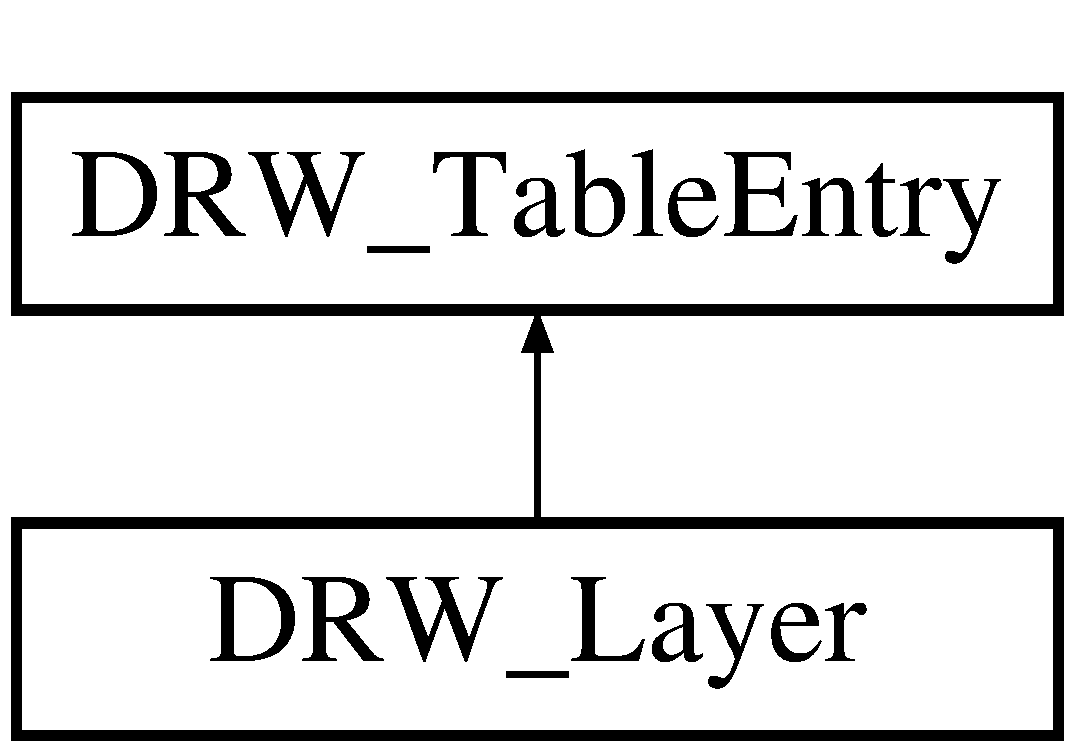
\includegraphics[height=2.000000cm]{d0/d63/class_d_r_w___layer}
\end{center}
\end{figure}
\subsection*{Public Member Functions}
\begin{DoxyCompactItemize}
\item 
void \hyperlink{class_d_r_w___layer_a3963fb621c29ebeac7b9a75159f37581}{parse\+Code} (int code, dxf\+Reader $\ast$reader)
\begin{DoxyCompactList}\small\item\em Class to handle layer entries. \end{DoxyCompactList}\end{DoxyCompactItemize}
\subsection*{Public Attributes}
\begin{DoxyCompactItemize}
\item 
U\+T\+F8\+S\+T\+R\+I\+N\+G \hyperlink{class_d_r_w___layer_a269aec5f78373fe152d83c39eca08ed0}{line\+Type}
\item 
int \hyperlink{class_d_r_w___layer_a9493b013d49446be87a1021086f7e17c}{color}
\item 
int \hyperlink{class_d_r_w___layer_a20e31ea14b3aff0194d862f06299fc98}{color24}
\item 
bool \hyperlink{class_d_r_w___layer_ac385c41055cb96d3c0ccb2938cb198f9}{plot\+F}
\item 
enum \hyperlink{class_d_r_w___l_w___conv_aed68cbc3d8bdf7e20003dd2d970279b3}{D\+R\+W\+\_\+\+L\+W\+\_\+\+Conv\+::line\+Width} \hyperlink{class_d_r_w___layer_a55dca2dbf071c0350a8b2aa3d9c5bfbd}{l\+Weight}
\item 
std\+::string \hyperlink{class_d_r_w___layer_ab158e3921f753cd59d6121f712062b9d}{handle\+Plot\+S}
\item 
std\+::string \hyperlink{class_d_r_w___layer_a67df26a8d8edf1cc26f62e3634c511ec}{handle\+Plot\+M}
\end{DoxyCompactItemize}
\subsection*{Additional Inherited Members}


\subsection{Detailed Description}
Class to handle layer entries. 

Class to handle layer symbol table entries \begin{DoxyAuthor}{Author}
Rallaz 
\end{DoxyAuthor}


\subsection{Member Function Documentation}
\hypertarget{class_d_r_w___layer_a3963fb621c29ebeac7b9a75159f37581}{}\index{D\+R\+W\+\_\+\+Layer@{D\+R\+W\+\_\+\+Layer}!parse\+Code@{parse\+Code}}
\index{parse\+Code@{parse\+Code}!D\+R\+W\+\_\+\+Layer@{D\+R\+W\+\_\+\+Layer}}
\subsubsection[{parse\+Code}]{\setlength{\rightskip}{0pt plus 5cm}void D\+R\+W\+\_\+\+Layer\+::parse\+Code (
\begin{DoxyParamCaption}
\item[{int}]{code, }
\item[{dxf\+Reader $\ast$}]{reader}
\end{DoxyParamCaption}
)}\label{class_d_r_w___layer_a3963fb621c29ebeac7b9a75159f37581}


Class to handle layer entries. 

Class to handle layer symbol table entries \begin{DoxyAuthor}{Author}
Rallaz 
\end{DoxyAuthor}


\subsection{Member Data Documentation}
\hypertarget{class_d_r_w___layer_a9493b013d49446be87a1021086f7e17c}{}\index{D\+R\+W\+\_\+\+Layer@{D\+R\+W\+\_\+\+Layer}!color@{color}}
\index{color@{color}!D\+R\+W\+\_\+\+Layer@{D\+R\+W\+\_\+\+Layer}}
\subsubsection[{color}]{\setlength{\rightskip}{0pt plus 5cm}int D\+R\+W\+\_\+\+Layer\+::color}\label{class_d_r_w___layer_a9493b013d49446be87a1021086f7e17c}
layer color, code 62 \hypertarget{class_d_r_w___layer_a20e31ea14b3aff0194d862f06299fc98}{}\index{D\+R\+W\+\_\+\+Layer@{D\+R\+W\+\_\+\+Layer}!color24@{color24}}
\index{color24@{color24}!D\+R\+W\+\_\+\+Layer@{D\+R\+W\+\_\+\+Layer}}
\subsubsection[{color24}]{\setlength{\rightskip}{0pt plus 5cm}int D\+R\+W\+\_\+\+Layer\+::color24}\label{class_d_r_w___layer_a20e31ea14b3aff0194d862f06299fc98}
24-\/bit color, code 420 \hypertarget{class_d_r_w___layer_a67df26a8d8edf1cc26f62e3634c511ec}{}\index{D\+R\+W\+\_\+\+Layer@{D\+R\+W\+\_\+\+Layer}!handle\+Plot\+M@{handle\+Plot\+M}}
\index{handle\+Plot\+M@{handle\+Plot\+M}!D\+R\+W\+\_\+\+Layer@{D\+R\+W\+\_\+\+Layer}}
\subsubsection[{handle\+Plot\+M}]{\setlength{\rightskip}{0pt plus 5cm}std\+::string D\+R\+W\+\_\+\+Layer\+::handle\+Plot\+M}\label{class_d_r_w___layer_a67df26a8d8edf1cc26f62e3634c511ec}
Hard-\/pointer I\+D/handle of materialstyle, code 347 \hypertarget{class_d_r_w___layer_ab158e3921f753cd59d6121f712062b9d}{}\index{D\+R\+W\+\_\+\+Layer@{D\+R\+W\+\_\+\+Layer}!handle\+Plot\+S@{handle\+Plot\+S}}
\index{handle\+Plot\+S@{handle\+Plot\+S}!D\+R\+W\+\_\+\+Layer@{D\+R\+W\+\_\+\+Layer}}
\subsubsection[{handle\+Plot\+S}]{\setlength{\rightskip}{0pt plus 5cm}std\+::string D\+R\+W\+\_\+\+Layer\+::handle\+Plot\+S}\label{class_d_r_w___layer_ab158e3921f753cd59d6121f712062b9d}
Hard-\/pointer I\+D/handle of plotstyle, code 390 \hypertarget{class_d_r_w___layer_a269aec5f78373fe152d83c39eca08ed0}{}\index{D\+R\+W\+\_\+\+Layer@{D\+R\+W\+\_\+\+Layer}!line\+Type@{line\+Type}}
\index{line\+Type@{line\+Type}!D\+R\+W\+\_\+\+Layer@{D\+R\+W\+\_\+\+Layer}}
\subsubsection[{line\+Type}]{\setlength{\rightskip}{0pt plus 5cm}U\+T\+F8\+S\+T\+R\+I\+N\+G D\+R\+W\+\_\+\+Layer\+::line\+Type}\label{class_d_r_w___layer_a269aec5f78373fe152d83c39eca08ed0}
line type, code 6 \hypertarget{class_d_r_w___layer_a55dca2dbf071c0350a8b2aa3d9c5bfbd}{}\index{D\+R\+W\+\_\+\+Layer@{D\+R\+W\+\_\+\+Layer}!l\+Weight@{l\+Weight}}
\index{l\+Weight@{l\+Weight}!D\+R\+W\+\_\+\+Layer@{D\+R\+W\+\_\+\+Layer}}
\subsubsection[{l\+Weight}]{\setlength{\rightskip}{0pt plus 5cm}enum {\bf D\+R\+W\+\_\+\+L\+W\+\_\+\+Conv\+::line\+Width} D\+R\+W\+\_\+\+Layer\+::l\+Weight}\label{class_d_r_w___layer_a55dca2dbf071c0350a8b2aa3d9c5bfbd}
layer lineweight, code 370 \hypertarget{class_d_r_w___layer_ac385c41055cb96d3c0ccb2938cb198f9}{}\index{D\+R\+W\+\_\+\+Layer@{D\+R\+W\+\_\+\+Layer}!plot\+F@{plot\+F}}
\index{plot\+F@{plot\+F}!D\+R\+W\+\_\+\+Layer@{D\+R\+W\+\_\+\+Layer}}
\subsubsection[{plot\+F}]{\setlength{\rightskip}{0pt plus 5cm}bool D\+R\+W\+\_\+\+Layer\+::plot\+F}\label{class_d_r_w___layer_ac385c41055cb96d3c0ccb2938cb198f9}
Plot flag, code 290 

The documentation for this class was generated from the following files\+:\begin{DoxyCompactItemize}
\item 
src/drw\+\_\+objects.\+h\item 
src/drw\+\_\+objects.\+cpp\end{DoxyCompactItemize}

\hypertarget{class_d_r_w___leader}{}\section{D\+R\+W\+\_\+\+Leader Class Reference}
\label{class_d_r_w___leader}\index{D\+R\+W\+\_\+\+Leader@{D\+R\+W\+\_\+\+Leader}}


Class to handle leader entity.  




{\ttfamily \#include $<$drw\+\_\+entities.\+h$>$}

Inheritance diagram for D\+R\+W\+\_\+\+Leader\+:\begin{figure}[H]
\begin{center}
\leavevmode
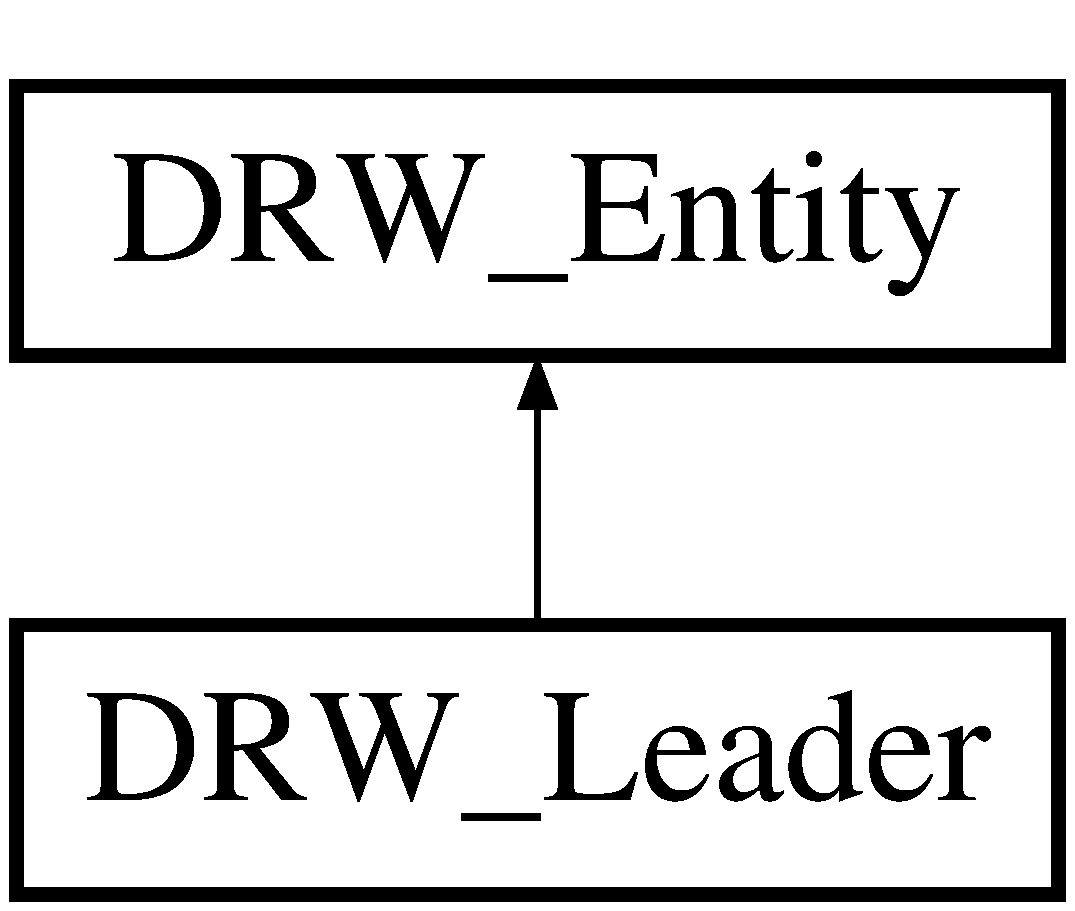
\includegraphics[height=2.000000cm]{d4/dfd/class_d_r_w___leader}
\end{center}
\end{figure}
\subsection*{Public Attributes}
\begin{DoxyCompactItemize}
\item 
U\+T\+F8\+S\+T\+R\+I\+N\+G \hyperlink{class_d_r_w___leader_a7a4e898ceae92208a03e86f7857e78e0}{style}
\item 
int \hyperlink{class_d_r_w___leader_a42f61a808411cf8465ec7f64c49cc4a6}{arrow}
\item 
int \hyperlink{class_d_r_w___leader_a4ba900b63165cb87b79612a9f9b4ff50}{leadertype}
\item 
int \hyperlink{class_d_r_w___leader_adcf19e8f9d127c910267e37a9d09e828}{flag}
\item 
int \hyperlink{class_d_r_w___leader_a80aca0277cc06cbcb4af9c6a42decf06}{hookline}
\item 
int \hyperlink{class_d_r_w___leader_a5d47804340900202fe3d1cd7bebbcecf}{hookflag}
\item 
double \hyperlink{class_d_r_w___leader_a5d4c5d32e962710240fc6ffa392c951b}{textheight}
\item 
double \hyperlink{class_d_r_w___leader_ab08450146f7f0658eca773a534d64be0}{textwidth}
\item 
int \hyperlink{class_d_r_w___leader_a8c0f8d7ebce1a2f1a4cb6d367a0c6a0d}{vertnum}
\item 
int \hyperlink{class_d_r_w___leader_afdff2ddfa67b8f2f46b367f52e06e027}{coloruse}
\item 
std\+::string \hyperlink{class_d_r_w___leader_a59ce8c8abeb1764ce3dbf042758d7cfa}{handle}
\item 
\hyperlink{class_d_r_w___coord}{D\+R\+W\+\_\+\+Coord} \hyperlink{class_d_r_w___leader_a9ef3ab714584747ac54612c47edd570a}{extrusion\+Point}
\item 
\hyperlink{class_d_r_w___coord}{D\+R\+W\+\_\+\+Coord} \hyperlink{class_d_r_w___leader_a31292925946b20b3c24f679c54f83523}{horizdir}
\item 
\hyperlink{class_d_r_w___coord}{D\+R\+W\+\_\+\+Coord} \hyperlink{class_d_r_w___leader_aa6a2e2b354365f405b52240c9bca3c8a}{offsetblock}
\item 
\hyperlink{class_d_r_w___coord}{D\+R\+W\+\_\+\+Coord} \hyperlink{class_d_r_w___leader_a6326c764bc74feaf7a5a3efa57325f67}{offsettext}
\item 
std\+::vector$<$ \hyperlink{class_d_r_w___coord}{D\+R\+W\+\_\+\+Coord} $\ast$ $>$ \hyperlink{class_d_r_w___leader_a7aef5bd8c0202b0c6836e15552866fcd}{vertexlist}
\end{DoxyCompactItemize}
\subsection*{Private Attributes}
\begin{DoxyCompactItemize}
\item 
\hyperlink{class_d_r_w___coord}{D\+R\+W\+\_\+\+Coord} $\ast$ \hyperlink{class_d_r_w___leader_a06568734914212d4d5fca83114459a2a}{vertexpoint}
\end{DoxyCompactItemize}
\subsection*{Friends}
\begin{DoxyCompactItemize}
\item 
\hypertarget{class_d_r_w___leader_a7f080e77e5112f8364c61b97387f8ee2}{}class {\bfseries dxf\+R\+W}\label{class_d_r_w___leader_a7f080e77e5112f8364c61b97387f8ee2}

\end{DoxyCompactItemize}
\subsection*{Additional Inherited Members}


\subsection{Detailed Description}
Class to handle leader entity. 

Class to handle leader entity \begin{DoxyAuthor}{Author}
Rallaz 
\end{DoxyAuthor}


\subsection{Member Data Documentation}
\hypertarget{class_d_r_w___leader_a42f61a808411cf8465ec7f64c49cc4a6}{}\index{D\+R\+W\+\_\+\+Leader@{D\+R\+W\+\_\+\+Leader}!arrow@{arrow}}
\index{arrow@{arrow}!D\+R\+W\+\_\+\+Leader@{D\+R\+W\+\_\+\+Leader}}
\subsubsection[{arrow}]{\setlength{\rightskip}{0pt plus 5cm}int D\+R\+W\+\_\+\+Leader\+::arrow}\label{class_d_r_w___leader_a42f61a808411cf8465ec7f64c49cc4a6}
Arrowhead flag, code 71, 0=Disabled; 1=Enabled \hypertarget{class_d_r_w___leader_afdff2ddfa67b8f2f46b367f52e06e027}{}\index{D\+R\+W\+\_\+\+Leader@{D\+R\+W\+\_\+\+Leader}!coloruse@{coloruse}}
\index{coloruse@{coloruse}!D\+R\+W\+\_\+\+Leader@{D\+R\+W\+\_\+\+Leader}}
\subsubsection[{coloruse}]{\setlength{\rightskip}{0pt plus 5cm}int D\+R\+W\+\_\+\+Leader\+::coloruse}\label{class_d_r_w___leader_afdff2ddfa67b8f2f46b367f52e06e027}
Color to use if leader\textquotesingle{}s D\+I\+M\+C\+L\+R\+D = B\+Y\+B\+L\+O\+C\+K, code 77 \hypertarget{class_d_r_w___leader_a9ef3ab714584747ac54612c47edd570a}{}\index{D\+R\+W\+\_\+\+Leader@{D\+R\+W\+\_\+\+Leader}!extrusion\+Point@{extrusion\+Point}}
\index{extrusion\+Point@{extrusion\+Point}!D\+R\+W\+\_\+\+Leader@{D\+R\+W\+\_\+\+Leader}}
\subsubsection[{extrusion\+Point}]{\setlength{\rightskip}{0pt plus 5cm}{\bf D\+R\+W\+\_\+\+Coord} D\+R\+W\+\_\+\+Leader\+::extrusion\+Point}\label{class_d_r_w___leader_a9ef3ab714584747ac54612c47edd570a}
Normal vector, code 210, 220 \& 230 \hypertarget{class_d_r_w___leader_adcf19e8f9d127c910267e37a9d09e828}{}\index{D\+R\+W\+\_\+\+Leader@{D\+R\+W\+\_\+\+Leader}!flag@{flag}}
\index{flag@{flag}!D\+R\+W\+\_\+\+Leader@{D\+R\+W\+\_\+\+Leader}}
\subsubsection[{flag}]{\setlength{\rightskip}{0pt plus 5cm}int D\+R\+W\+\_\+\+Leader\+::flag}\label{class_d_r_w___leader_adcf19e8f9d127c910267e37a9d09e828}
Leader creation flag, code 73, default 3 \hypertarget{class_d_r_w___leader_a59ce8c8abeb1764ce3dbf042758d7cfa}{}\index{D\+R\+W\+\_\+\+Leader@{D\+R\+W\+\_\+\+Leader}!handle@{handle}}
\index{handle@{handle}!D\+R\+W\+\_\+\+Leader@{D\+R\+W\+\_\+\+Leader}}
\subsubsection[{handle}]{\setlength{\rightskip}{0pt plus 5cm}std\+::string D\+R\+W\+\_\+\+Leader\+::handle}\label{class_d_r_w___leader_a59ce8c8abeb1764ce3dbf042758d7cfa}
Hard reference to associated annotation, code 340 \hypertarget{class_d_r_w___leader_a5d47804340900202fe3d1cd7bebbcecf}{}\index{D\+R\+W\+\_\+\+Leader@{D\+R\+W\+\_\+\+Leader}!hookflag@{hookflag}}
\index{hookflag@{hookflag}!D\+R\+W\+\_\+\+Leader@{D\+R\+W\+\_\+\+Leader}}
\subsubsection[{hookflag}]{\setlength{\rightskip}{0pt plus 5cm}int D\+R\+W\+\_\+\+Leader\+::hookflag}\label{class_d_r_w___leader_a5d47804340900202fe3d1cd7bebbcecf}
Hook line flag, code 75 \hypertarget{class_d_r_w___leader_a80aca0277cc06cbcb4af9c6a42decf06}{}\index{D\+R\+W\+\_\+\+Leader@{D\+R\+W\+\_\+\+Leader}!hookline@{hookline}}
\index{hookline@{hookline}!D\+R\+W\+\_\+\+Leader@{D\+R\+W\+\_\+\+Leader}}
\subsubsection[{hookline}]{\setlength{\rightskip}{0pt plus 5cm}int D\+R\+W\+\_\+\+Leader\+::hookline}\label{class_d_r_w___leader_a80aca0277cc06cbcb4af9c6a42decf06}
Hook line direction flag, code 74, default 1 \hypertarget{class_d_r_w___leader_a31292925946b20b3c24f679c54f83523}{}\index{D\+R\+W\+\_\+\+Leader@{D\+R\+W\+\_\+\+Leader}!horizdir@{horizdir}}
\index{horizdir@{horizdir}!D\+R\+W\+\_\+\+Leader@{D\+R\+W\+\_\+\+Leader}}
\subsubsection[{horizdir}]{\setlength{\rightskip}{0pt plus 5cm}{\bf D\+R\+W\+\_\+\+Coord} D\+R\+W\+\_\+\+Leader\+::horizdir}\label{class_d_r_w___leader_a31292925946b20b3c24f679c54f83523}
\char`\"{}\+Horizontal\char`\"{} direction for leader, code 211, 221 \& 231 \hypertarget{class_d_r_w___leader_a4ba900b63165cb87b79612a9f9b4ff50}{}\index{D\+R\+W\+\_\+\+Leader@{D\+R\+W\+\_\+\+Leader}!leadertype@{leadertype}}
\index{leadertype@{leadertype}!D\+R\+W\+\_\+\+Leader@{D\+R\+W\+\_\+\+Leader}}
\subsubsection[{leadertype}]{\setlength{\rightskip}{0pt plus 5cm}int D\+R\+W\+\_\+\+Leader\+::leadertype}\label{class_d_r_w___leader_a4ba900b63165cb87b79612a9f9b4ff50}
Leader path type, code 72, 0=Straight line segments; 1=Spline \hypertarget{class_d_r_w___leader_aa6a2e2b354365f405b52240c9bca3c8a}{}\index{D\+R\+W\+\_\+\+Leader@{D\+R\+W\+\_\+\+Leader}!offsetblock@{offsetblock}}
\index{offsetblock@{offsetblock}!D\+R\+W\+\_\+\+Leader@{D\+R\+W\+\_\+\+Leader}}
\subsubsection[{offsetblock}]{\setlength{\rightskip}{0pt plus 5cm}{\bf D\+R\+W\+\_\+\+Coord} D\+R\+W\+\_\+\+Leader\+::offsetblock}\label{class_d_r_w___leader_aa6a2e2b354365f405b52240c9bca3c8a}
Offset of last leader vertex from block, code 212, 222 \& 232 \hypertarget{class_d_r_w___leader_a6326c764bc74feaf7a5a3efa57325f67}{}\index{D\+R\+W\+\_\+\+Leader@{D\+R\+W\+\_\+\+Leader}!offsettext@{offsettext}}
\index{offsettext@{offsettext}!D\+R\+W\+\_\+\+Leader@{D\+R\+W\+\_\+\+Leader}}
\subsubsection[{offsettext}]{\setlength{\rightskip}{0pt plus 5cm}{\bf D\+R\+W\+\_\+\+Coord} D\+R\+W\+\_\+\+Leader\+::offsettext}\label{class_d_r_w___leader_a6326c764bc74feaf7a5a3efa57325f67}
Offset of last leader vertex from annotation, code 213, 223 \& 233 \hypertarget{class_d_r_w___leader_a7a4e898ceae92208a03e86f7857e78e0}{}\index{D\+R\+W\+\_\+\+Leader@{D\+R\+W\+\_\+\+Leader}!style@{style}}
\index{style@{style}!D\+R\+W\+\_\+\+Leader@{D\+R\+W\+\_\+\+Leader}}
\subsubsection[{style}]{\setlength{\rightskip}{0pt plus 5cm}U\+T\+F8\+S\+T\+R\+I\+N\+G D\+R\+W\+\_\+\+Leader\+::style}\label{class_d_r_w___leader_a7a4e898ceae92208a03e86f7857e78e0}
Dimension style name, code 3 \hypertarget{class_d_r_w___leader_a5d4c5d32e962710240fc6ffa392c951b}{}\index{D\+R\+W\+\_\+\+Leader@{D\+R\+W\+\_\+\+Leader}!textheight@{textheight}}
\index{textheight@{textheight}!D\+R\+W\+\_\+\+Leader@{D\+R\+W\+\_\+\+Leader}}
\subsubsection[{textheight}]{\setlength{\rightskip}{0pt plus 5cm}double D\+R\+W\+\_\+\+Leader\+::textheight}\label{class_d_r_w___leader_a5d4c5d32e962710240fc6ffa392c951b}
Text annotation height, code 40 \hypertarget{class_d_r_w___leader_ab08450146f7f0658eca773a534d64be0}{}\index{D\+R\+W\+\_\+\+Leader@{D\+R\+W\+\_\+\+Leader}!textwidth@{textwidth}}
\index{textwidth@{textwidth}!D\+R\+W\+\_\+\+Leader@{D\+R\+W\+\_\+\+Leader}}
\subsubsection[{textwidth}]{\setlength{\rightskip}{0pt plus 5cm}double D\+R\+W\+\_\+\+Leader\+::textwidth}\label{class_d_r_w___leader_ab08450146f7f0658eca773a534d64be0}
Text annotation width, code 41 \hypertarget{class_d_r_w___leader_a7aef5bd8c0202b0c6836e15552866fcd}{}\index{D\+R\+W\+\_\+\+Leader@{D\+R\+W\+\_\+\+Leader}!vertexlist@{vertexlist}}
\index{vertexlist@{vertexlist}!D\+R\+W\+\_\+\+Leader@{D\+R\+W\+\_\+\+Leader}}
\subsubsection[{vertexlist}]{\setlength{\rightskip}{0pt plus 5cm}std\+::vector$<${\bf D\+R\+W\+\_\+\+Coord} $\ast$$>$ D\+R\+W\+\_\+\+Leader\+::vertexlist}\label{class_d_r_w___leader_a7aef5bd8c0202b0c6836e15552866fcd}
vertex points list, code 10, 20 \& 30 \hypertarget{class_d_r_w___leader_a06568734914212d4d5fca83114459a2a}{}\index{D\+R\+W\+\_\+\+Leader@{D\+R\+W\+\_\+\+Leader}!vertexpoint@{vertexpoint}}
\index{vertexpoint@{vertexpoint}!D\+R\+W\+\_\+\+Leader@{D\+R\+W\+\_\+\+Leader}}
\subsubsection[{vertexpoint}]{\setlength{\rightskip}{0pt plus 5cm}{\bf D\+R\+W\+\_\+\+Coord}$\ast$ D\+R\+W\+\_\+\+Leader\+::vertexpoint\hspace{0.3cm}{\ttfamily [private]}}\label{class_d_r_w___leader_a06568734914212d4d5fca83114459a2a}
current control point to add data \hypertarget{class_d_r_w___leader_a8c0f8d7ebce1a2f1a4cb6d367a0c6a0d}{}\index{D\+R\+W\+\_\+\+Leader@{D\+R\+W\+\_\+\+Leader}!vertnum@{vertnum}}
\index{vertnum@{vertnum}!D\+R\+W\+\_\+\+Leader@{D\+R\+W\+\_\+\+Leader}}
\subsubsection[{vertnum}]{\setlength{\rightskip}{0pt plus 5cm}int D\+R\+W\+\_\+\+Leader\+::vertnum}\label{class_d_r_w___leader_a8c0f8d7ebce1a2f1a4cb6d367a0c6a0d}
Number of vertices, code 76 

The documentation for this class was generated from the following files\+:\begin{DoxyCompactItemize}
\item 
src/drw\+\_\+entities.\+h\item 
src/drw\+\_\+entities.\+cpp\end{DoxyCompactItemize}

\hypertarget{class_d_r_w___line}{}\section{D\+R\+W\+\_\+\+Line Class Reference}
\label{class_d_r_w___line}\index{D\+R\+W\+\_\+\+Line@{D\+R\+W\+\_\+\+Line}}


Class to handle line entity.  




{\ttfamily \#include $<$drw\+\_\+entities.\+h$>$}

Inheritance diagram for D\+R\+W\+\_\+\+Line\+:\begin{figure}[H]
\begin{center}
\leavevmode
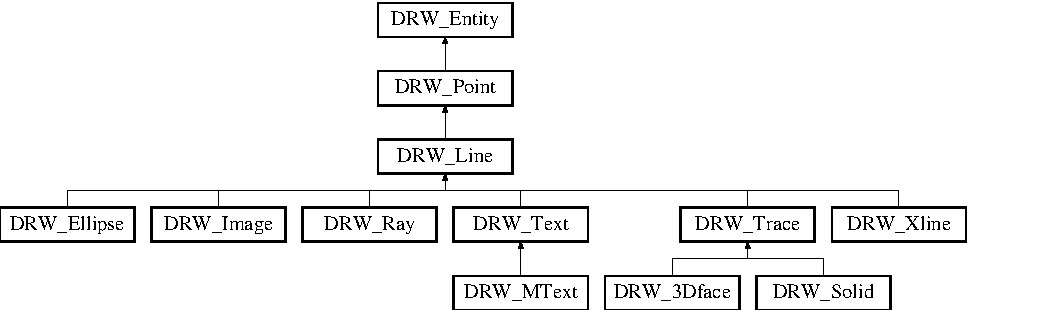
\includegraphics[height=4.166667cm]{d8/dc4/class_d_r_w___line}
\end{center}
\end{figure}
\subsection*{Public Attributes}
\begin{DoxyCompactItemize}
\item 
\hyperlink{class_d_r_w___coord}{D\+R\+W\+\_\+\+Coord} \hyperlink{class_d_r_w___line_afba62212864227b610be3e2a4e7ac307}{sec\+Point}
\end{DoxyCompactItemize}
\subsection*{Additional Inherited Members}


\subsection{Detailed Description}
Class to handle line entity. 

Class to handle line entity \begin{DoxyAuthor}{Author}
Rallaz 
\end{DoxyAuthor}


\subsection{Member Data Documentation}
\hypertarget{class_d_r_w___line_afba62212864227b610be3e2a4e7ac307}{}\index{D\+R\+W\+\_\+\+Line@{D\+R\+W\+\_\+\+Line}!sec\+Point@{sec\+Point}}
\index{sec\+Point@{sec\+Point}!D\+R\+W\+\_\+\+Line@{D\+R\+W\+\_\+\+Line}}
\subsubsection[{sec\+Point}]{\setlength{\rightskip}{0pt plus 5cm}{\bf D\+R\+W\+\_\+\+Coord} D\+R\+W\+\_\+\+Line\+::sec\+Point}\label{class_d_r_w___line_afba62212864227b610be3e2a4e7ac307}
second point, code 11, 21 \& 31 

The documentation for this class was generated from the following files\+:\begin{DoxyCompactItemize}
\item 
src/drw\+\_\+entities.\+h\item 
src/drw\+\_\+entities.\+cpp\end{DoxyCompactItemize}

\hypertarget{class_d_r_w___l_type}{}\section{D\+R\+W\+\_\+\+L\+Type Class Reference}
\label{class_d_r_w___l_type}\index{D\+R\+W\+\_\+\+L\+Type@{D\+R\+W\+\_\+\+L\+Type}}


Class to handle line type entries.  




{\ttfamily \#include $<$drw\+\_\+objects.\+h$>$}

Inheritance diagram for D\+R\+W\+\_\+\+L\+Type\+:\begin{figure}[H]
\begin{center}
\leavevmode
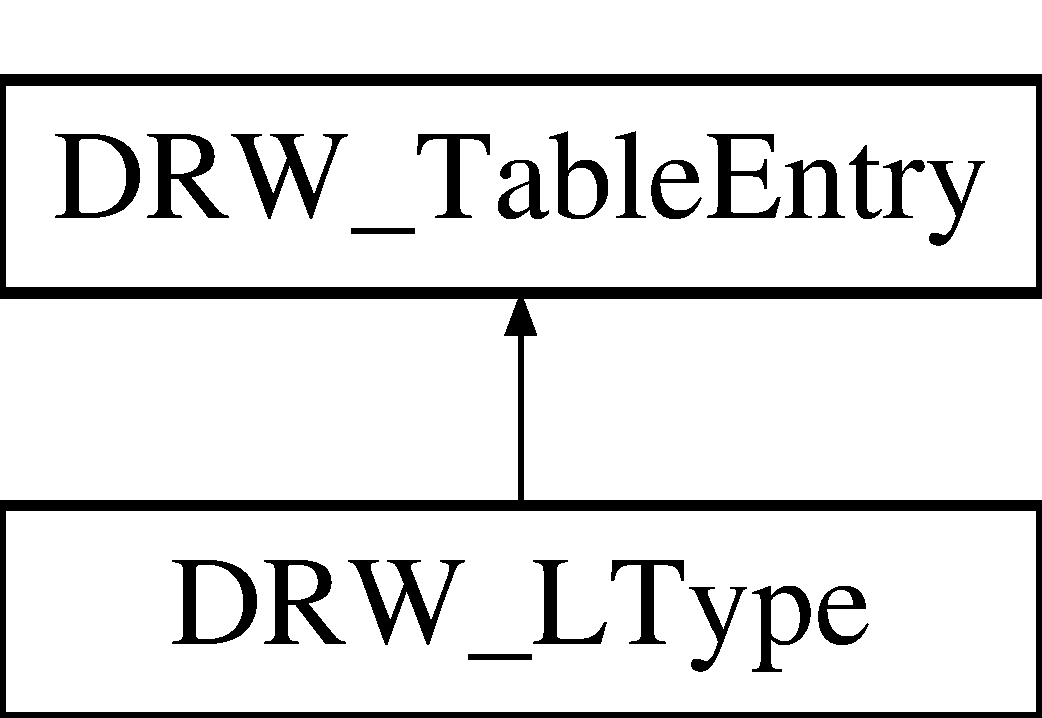
\includegraphics[height=2.000000cm]{d4/dcc/class_d_r_w___l_type}
\end{center}
\end{figure}
\subsection*{Public Member Functions}
\begin{DoxyCompactItemize}
\item 
void \hyperlink{class_d_r_w___l_type_a7c1bcdc02c5aa43262221ad55dfac6ff}{parse\+Code} (int code, dxf\+Reader $\ast$reader)
\begin{DoxyCompactList}\small\item\em Class to handle line type entries. \end{DoxyCompactList}\item 
void \hyperlink{class_d_r_w___l_type_a9cebdfa5d1ae14720c4fcd50f45dab5a}{update} ()
\begin{DoxyCompactList}\small\item\em Update line type. \end{DoxyCompactList}\end{DoxyCompactItemize}
\subsection*{Public Attributes}
\begin{DoxyCompactItemize}
\item 
U\+T\+F8\+S\+T\+R\+I\+N\+G \hyperlink{class_d_r_w___l_type_ae6f6458c8c9ac100908259558c7e22d2}{desc}
\item 
int \hyperlink{class_d_r_w___l_type_acb78cd0a105ac8b44e19313a4bf90f50}{size}
\item 
double \hyperlink{class_d_r_w___l_type_a438510524566f0deaf77ea694f171762}{length}
\item 
std\+::vector$<$ double $>$ \hyperlink{class_d_r_w___l_type_afb0702d3edab2948fdba2fb861fd3a4b}{path}
\end{DoxyCompactItemize}
\subsection*{Additional Inherited Members}


\subsection{Detailed Description}
Class to handle line type entries. 

Class to handle line type symbol table entries \begin{DoxyAuthor}{Author}
Rallaz 
\end{DoxyAuthor}


\subsection{Member Function Documentation}
\hypertarget{class_d_r_w___l_type_a7c1bcdc02c5aa43262221ad55dfac6ff}{}\index{D\+R\+W\+\_\+\+L\+Type@{D\+R\+W\+\_\+\+L\+Type}!parse\+Code@{parse\+Code}}
\index{parse\+Code@{parse\+Code}!D\+R\+W\+\_\+\+L\+Type@{D\+R\+W\+\_\+\+L\+Type}}
\subsubsection[{parse\+Code}]{\setlength{\rightskip}{0pt plus 5cm}void D\+R\+W\+\_\+\+L\+Type\+::parse\+Code (
\begin{DoxyParamCaption}
\item[{int}]{code, }
\item[{dxf\+Reader $\ast$}]{reader}
\end{DoxyParamCaption}
)}\label{class_d_r_w___l_type_a7c1bcdc02c5aa43262221ad55dfac6ff}


Class to handle line type entries. 

Class to handle line type symbol table entries \begin{DoxyAuthor}{Author}
Rallaz 
\end{DoxyAuthor}
\hypertarget{class_d_r_w___l_type_a9cebdfa5d1ae14720c4fcd50f45dab5a}{}\index{D\+R\+W\+\_\+\+L\+Type@{D\+R\+W\+\_\+\+L\+Type}!update@{update}}
\index{update@{update}!D\+R\+W\+\_\+\+L\+Type@{D\+R\+W\+\_\+\+L\+Type}}
\subsubsection[{update}]{\setlength{\rightskip}{0pt plus 5cm}void D\+R\+W\+\_\+\+L\+Type\+::update (
\begin{DoxyParamCaption}
{}
\end{DoxyParamCaption}
)}\label{class_d_r_w___l_type_a9cebdfa5d1ae14720c4fcd50f45dab5a}


Update line type. 

Update the size and length of line type acording to the path \begin{DoxyAuthor}{Author}
Rallaz 
\end{DoxyAuthor}


\subsection{Member Data Documentation}
\hypertarget{class_d_r_w___l_type_ae6f6458c8c9ac100908259558c7e22d2}{}\index{D\+R\+W\+\_\+\+L\+Type@{D\+R\+W\+\_\+\+L\+Type}!desc@{desc}}
\index{desc@{desc}!D\+R\+W\+\_\+\+L\+Type@{D\+R\+W\+\_\+\+L\+Type}}
\subsubsection[{desc}]{\setlength{\rightskip}{0pt plus 5cm}U\+T\+F8\+S\+T\+R\+I\+N\+G D\+R\+W\+\_\+\+L\+Type\+::desc}\label{class_d_r_w___l_type_ae6f6458c8c9ac100908259558c7e22d2}
descriptive string, code 3 \hypertarget{class_d_r_w___l_type_a438510524566f0deaf77ea694f171762}{}\index{D\+R\+W\+\_\+\+L\+Type@{D\+R\+W\+\_\+\+L\+Type}!length@{length}}
\index{length@{length}!D\+R\+W\+\_\+\+L\+Type@{D\+R\+W\+\_\+\+L\+Type}}
\subsubsection[{length}]{\setlength{\rightskip}{0pt plus 5cm}double D\+R\+W\+\_\+\+L\+Type\+::length}\label{class_d_r_w___l_type_a438510524566f0deaf77ea694f171762}
total length of pattern, code 40 \hypertarget{class_d_r_w___l_type_afb0702d3edab2948fdba2fb861fd3a4b}{}\index{D\+R\+W\+\_\+\+L\+Type@{D\+R\+W\+\_\+\+L\+Type}!path@{path}}
\index{path@{path}!D\+R\+W\+\_\+\+L\+Type@{D\+R\+W\+\_\+\+L\+Type}}
\subsubsection[{path}]{\setlength{\rightskip}{0pt plus 5cm}std\+::vector$<$double$>$ D\+R\+W\+\_\+\+L\+Type\+::path}\label{class_d_r_w___l_type_afb0702d3edab2948fdba2fb861fd3a4b}
trace, point or space length sequence, code 49 \hypertarget{class_d_r_w___l_type_acb78cd0a105ac8b44e19313a4bf90f50}{}\index{D\+R\+W\+\_\+\+L\+Type@{D\+R\+W\+\_\+\+L\+Type}!size@{size}}
\index{size@{size}!D\+R\+W\+\_\+\+L\+Type@{D\+R\+W\+\_\+\+L\+Type}}
\subsubsection[{size}]{\setlength{\rightskip}{0pt plus 5cm}int D\+R\+W\+\_\+\+L\+Type\+::size}\label{class_d_r_w___l_type_acb78cd0a105ac8b44e19313a4bf90f50}
element number, code 73 

The documentation for this class was generated from the following files\+:\begin{DoxyCompactItemize}
\item 
src/drw\+\_\+objects.\+h\item 
src/drw\+\_\+objects.\+cpp\end{DoxyCompactItemize}

\hypertarget{class_d_r_w___l_w___conv}{}\section{D\+R\+W\+\_\+\+L\+W\+\_\+\+Conv Class Reference}
\label{class_d_r_w___l_w___conv}\index{D\+R\+W\+\_\+\+L\+W\+\_\+\+Conv@{D\+R\+W\+\_\+\+L\+W\+\_\+\+Conv}}


Class to convert between line width and integer.  




{\ttfamily \#include $<$drw\+\_\+base.\+h$>$}

\subsection*{Public Types}
\begin{DoxyCompactItemize}
\item 
enum \hyperlink{class_d_r_w___l_w___conv_aed68cbc3d8bdf7e20003dd2d970279b3}{line\+Width} \{ \\*
\hyperlink{class_d_r_w___l_w___conv_aed68cbc3d8bdf7e20003dd2d970279b3a3007c229abfe3c9f018b2a881384aa17}{width00} = 0, 
\hyperlink{class_d_r_w___l_w___conv_aed68cbc3d8bdf7e20003dd2d970279b3a27fc91eb33b8254bd0d0fbbb4b9430cc}{width01} = 1, 
\hyperlink{class_d_r_w___l_w___conv_aed68cbc3d8bdf7e20003dd2d970279b3aa85257cc5f5a011103273232c4f90822}{width02} = 2, 
\hyperlink{class_d_r_w___l_w___conv_aed68cbc3d8bdf7e20003dd2d970279b3ac0b97f9dfaf10daada26307bee172b82}{width03} = 3, 
\\*
\hyperlink{class_d_r_w___l_w___conv_aed68cbc3d8bdf7e20003dd2d970279b3a5f4b9dfe971a491e4250eb79e80cb603}{width04} = 4, 
\hyperlink{class_d_r_w___l_w___conv_aed68cbc3d8bdf7e20003dd2d970279b3acd3977a246f53b52046f215069e3a2bb}{width05} = 5, 
\hyperlink{class_d_r_w___l_w___conv_aed68cbc3d8bdf7e20003dd2d970279b3a770acce0ba10abcb50783062e464201d}{width06} = 6, 
\hyperlink{class_d_r_w___l_w___conv_aed68cbc3d8bdf7e20003dd2d970279b3a8c6d299834725dad1281e866f530dad2}{width07} = 7, 
\\*
\hyperlink{class_d_r_w___l_w___conv_aed68cbc3d8bdf7e20003dd2d970279b3a8b4ebbd7b5fa5f360907e53d4c3ef7a4}{width08} = 8, 
\hyperlink{class_d_r_w___l_w___conv_aed68cbc3d8bdf7e20003dd2d970279b3a9a8782efdcc8d0a6eb6400f05a9cb082}{width09} = 9, 
\hyperlink{class_d_r_w___l_w___conv_aed68cbc3d8bdf7e20003dd2d970279b3a90804835ca340953071b6aaf6fea9f9c}{width10} = 10, 
\hyperlink{class_d_r_w___l_w___conv_aed68cbc3d8bdf7e20003dd2d970279b3ad2ffa082a10ec1a0681f58db93ad4e92}{width11} = 11, 
\\*
\hyperlink{class_d_r_w___l_w___conv_aed68cbc3d8bdf7e20003dd2d970279b3aff60246d9f43ab88f2a128a6755522df}{width12} = 12, 
\hyperlink{class_d_r_w___l_w___conv_aed68cbc3d8bdf7e20003dd2d970279b3ab270b1411e0a8cfb209793262b208c9e}{width13} = 13, 
\hyperlink{class_d_r_w___l_w___conv_aed68cbc3d8bdf7e20003dd2d970279b3a0b462588b45aae5b31989c248c9fb8ec}{width14} = 14, 
\hyperlink{class_d_r_w___l_w___conv_aed68cbc3d8bdf7e20003dd2d970279b3ab7cdf855ca689fb9b91a3795222cd824}{width15} = 15, 
\\*
\hyperlink{class_d_r_w___l_w___conv_aed68cbc3d8bdf7e20003dd2d970279b3abce2c49577a99240fb9562c61724e6ff}{width16} = 16, 
\hyperlink{class_d_r_w___l_w___conv_aed68cbc3d8bdf7e20003dd2d970279b3a095b12d03a51c0da42e0d34a4595e680}{width17} = 17, 
\hyperlink{class_d_r_w___l_w___conv_aed68cbc3d8bdf7e20003dd2d970279b3a57b59dd1e97e6a0af349309e997c3ab7}{width18} = 18, 
\hyperlink{class_d_r_w___l_w___conv_aed68cbc3d8bdf7e20003dd2d970279b3a2a0d3619f28ed9caa63175a90a523812}{width19} = 19, 
\\*
\hyperlink{class_d_r_w___l_w___conv_aed68cbc3d8bdf7e20003dd2d970279b3aa9b310ae50f3e6389e5d2687bc3d9659}{width20} = 20, 
\hyperlink{class_d_r_w___l_w___conv_aed68cbc3d8bdf7e20003dd2d970279b3a5cc5d000ea38449bd040384e181e6379}{width21} = 21, 
\hyperlink{class_d_r_w___l_w___conv_aed68cbc3d8bdf7e20003dd2d970279b3a4e2f7d51662ebe7647c8fa3e853b281f}{width22} = 22, 
\hyperlink{class_d_r_w___l_w___conv_aed68cbc3d8bdf7e20003dd2d970279b3a211d736ceb1820badf30039652355ba0}{width23} = 23, 
\\*
\hyperlink{class_d_r_w___l_w___conv_aed68cbc3d8bdf7e20003dd2d970279b3ac5d0d3025329964b2ea07f29131a50e8}{width\+By\+Layer} = 29, 
\hyperlink{class_d_r_w___l_w___conv_aed68cbc3d8bdf7e20003dd2d970279b3a11fd9dfa615187c6237b092ebfe4330b}{width\+By\+Block} = 30, 
\hyperlink{class_d_r_w___l_w___conv_aed68cbc3d8bdf7e20003dd2d970279b3a2a30bb15248d15595514d75d34e5afd5}{width\+Default} = 31
 \}
\end{DoxyCompactItemize}


\subsection{Detailed Description}
Class to convert between line width and integer. 

Class to convert between line width and integer verifing valid values, if value is not valid returns width\+Default. \begin{DoxyAuthor}{Author}
Rallaz 
\end{DoxyAuthor}


\subsection{Member Enumeration Documentation}
\hypertarget{class_d_r_w___l_w___conv_aed68cbc3d8bdf7e20003dd2d970279b3}{}\index{D\+R\+W\+\_\+\+L\+W\+\_\+\+Conv@{D\+R\+W\+\_\+\+L\+W\+\_\+\+Conv}!line\+Width@{line\+Width}}
\index{line\+Width@{line\+Width}!D\+R\+W\+\_\+\+L\+W\+\_\+\+Conv@{D\+R\+W\+\_\+\+L\+W\+\_\+\+Conv}}
\subsubsection[{line\+Width}]{\setlength{\rightskip}{0pt plus 5cm}enum {\bf D\+R\+W\+\_\+\+L\+W\+\_\+\+Conv\+::line\+Width}}\label{class_d_r_w___l_w___conv_aed68cbc3d8bdf7e20003dd2d970279b3}
\begin{Desc}
\item[Enumerator]\par
\begin{description}
\index{width00@{width00}!D\+R\+W\+\_\+\+L\+W\+\_\+\+Conv@{D\+R\+W\+\_\+\+L\+W\+\_\+\+Conv}}\index{D\+R\+W\+\_\+\+L\+W\+\_\+\+Conv@{D\+R\+W\+\_\+\+L\+W\+\_\+\+Conv}!width00@{width00}}\item[{\em 
\hypertarget{class_d_r_w___l_w___conv_aed68cbc3d8bdf7e20003dd2d970279b3a3007c229abfe3c9f018b2a881384aa17}{}width00\label{class_d_r_w___l_w___conv_aed68cbc3d8bdf7e20003dd2d970279b3a3007c229abfe3c9f018b2a881384aa17}
}]0.\+00mm (dxf 0) \index{width01@{width01}!D\+R\+W\+\_\+\+L\+W\+\_\+\+Conv@{D\+R\+W\+\_\+\+L\+W\+\_\+\+Conv}}\index{D\+R\+W\+\_\+\+L\+W\+\_\+\+Conv@{D\+R\+W\+\_\+\+L\+W\+\_\+\+Conv}!width01@{width01}}\item[{\em 
\hypertarget{class_d_r_w___l_w___conv_aed68cbc3d8bdf7e20003dd2d970279b3a27fc91eb33b8254bd0d0fbbb4b9430cc}{}width01\label{class_d_r_w___l_w___conv_aed68cbc3d8bdf7e20003dd2d970279b3a27fc91eb33b8254bd0d0fbbb4b9430cc}
}]0.\+05mm (dxf 5) \index{width02@{width02}!D\+R\+W\+\_\+\+L\+W\+\_\+\+Conv@{D\+R\+W\+\_\+\+L\+W\+\_\+\+Conv}}\index{D\+R\+W\+\_\+\+L\+W\+\_\+\+Conv@{D\+R\+W\+\_\+\+L\+W\+\_\+\+Conv}!width02@{width02}}\item[{\em 
\hypertarget{class_d_r_w___l_w___conv_aed68cbc3d8bdf7e20003dd2d970279b3aa85257cc5f5a011103273232c4f90822}{}width02\label{class_d_r_w___l_w___conv_aed68cbc3d8bdf7e20003dd2d970279b3aa85257cc5f5a011103273232c4f90822}
}]0.\+09mm (dxf 9) \index{width03@{width03}!D\+R\+W\+\_\+\+L\+W\+\_\+\+Conv@{D\+R\+W\+\_\+\+L\+W\+\_\+\+Conv}}\index{D\+R\+W\+\_\+\+L\+W\+\_\+\+Conv@{D\+R\+W\+\_\+\+L\+W\+\_\+\+Conv}!width03@{width03}}\item[{\em 
\hypertarget{class_d_r_w___l_w___conv_aed68cbc3d8bdf7e20003dd2d970279b3ac0b97f9dfaf10daada26307bee172b82}{}width03\label{class_d_r_w___l_w___conv_aed68cbc3d8bdf7e20003dd2d970279b3ac0b97f9dfaf10daada26307bee172b82}
}]0.\+13mm (dxf 13) \index{width04@{width04}!D\+R\+W\+\_\+\+L\+W\+\_\+\+Conv@{D\+R\+W\+\_\+\+L\+W\+\_\+\+Conv}}\index{D\+R\+W\+\_\+\+L\+W\+\_\+\+Conv@{D\+R\+W\+\_\+\+L\+W\+\_\+\+Conv}!width04@{width04}}\item[{\em 
\hypertarget{class_d_r_w___l_w___conv_aed68cbc3d8bdf7e20003dd2d970279b3a5f4b9dfe971a491e4250eb79e80cb603}{}width04\label{class_d_r_w___l_w___conv_aed68cbc3d8bdf7e20003dd2d970279b3a5f4b9dfe971a491e4250eb79e80cb603}
}]0.\+15mm (dxf 15) \index{width05@{width05}!D\+R\+W\+\_\+\+L\+W\+\_\+\+Conv@{D\+R\+W\+\_\+\+L\+W\+\_\+\+Conv}}\index{D\+R\+W\+\_\+\+L\+W\+\_\+\+Conv@{D\+R\+W\+\_\+\+L\+W\+\_\+\+Conv}!width05@{width05}}\item[{\em 
\hypertarget{class_d_r_w___l_w___conv_aed68cbc3d8bdf7e20003dd2d970279b3acd3977a246f53b52046f215069e3a2bb}{}width05\label{class_d_r_w___l_w___conv_aed68cbc3d8bdf7e20003dd2d970279b3acd3977a246f53b52046f215069e3a2bb}
}]0.\+18mm (dxf 18) \index{width06@{width06}!D\+R\+W\+\_\+\+L\+W\+\_\+\+Conv@{D\+R\+W\+\_\+\+L\+W\+\_\+\+Conv}}\index{D\+R\+W\+\_\+\+L\+W\+\_\+\+Conv@{D\+R\+W\+\_\+\+L\+W\+\_\+\+Conv}!width06@{width06}}\item[{\em 
\hypertarget{class_d_r_w___l_w___conv_aed68cbc3d8bdf7e20003dd2d970279b3a770acce0ba10abcb50783062e464201d}{}width06\label{class_d_r_w___l_w___conv_aed68cbc3d8bdf7e20003dd2d970279b3a770acce0ba10abcb50783062e464201d}
}]0.\+20mm (dxf 20) \index{width07@{width07}!D\+R\+W\+\_\+\+L\+W\+\_\+\+Conv@{D\+R\+W\+\_\+\+L\+W\+\_\+\+Conv}}\index{D\+R\+W\+\_\+\+L\+W\+\_\+\+Conv@{D\+R\+W\+\_\+\+L\+W\+\_\+\+Conv}!width07@{width07}}\item[{\em 
\hypertarget{class_d_r_w___l_w___conv_aed68cbc3d8bdf7e20003dd2d970279b3a8c6d299834725dad1281e866f530dad2}{}width07\label{class_d_r_w___l_w___conv_aed68cbc3d8bdf7e20003dd2d970279b3a8c6d299834725dad1281e866f530dad2}
}]0.\+25mm (dxf 25) \index{width08@{width08}!D\+R\+W\+\_\+\+L\+W\+\_\+\+Conv@{D\+R\+W\+\_\+\+L\+W\+\_\+\+Conv}}\index{D\+R\+W\+\_\+\+L\+W\+\_\+\+Conv@{D\+R\+W\+\_\+\+L\+W\+\_\+\+Conv}!width08@{width08}}\item[{\em 
\hypertarget{class_d_r_w___l_w___conv_aed68cbc3d8bdf7e20003dd2d970279b3a8b4ebbd7b5fa5f360907e53d4c3ef7a4}{}width08\label{class_d_r_w___l_w___conv_aed68cbc3d8bdf7e20003dd2d970279b3a8b4ebbd7b5fa5f360907e53d4c3ef7a4}
}]0.\+30mm (dxf 30) \index{width09@{width09}!D\+R\+W\+\_\+\+L\+W\+\_\+\+Conv@{D\+R\+W\+\_\+\+L\+W\+\_\+\+Conv}}\index{D\+R\+W\+\_\+\+L\+W\+\_\+\+Conv@{D\+R\+W\+\_\+\+L\+W\+\_\+\+Conv}!width09@{width09}}\item[{\em 
\hypertarget{class_d_r_w___l_w___conv_aed68cbc3d8bdf7e20003dd2d970279b3a9a8782efdcc8d0a6eb6400f05a9cb082}{}width09\label{class_d_r_w___l_w___conv_aed68cbc3d8bdf7e20003dd2d970279b3a9a8782efdcc8d0a6eb6400f05a9cb082}
}]0.\+35mm (dxf 35) \index{width10@{width10}!D\+R\+W\+\_\+\+L\+W\+\_\+\+Conv@{D\+R\+W\+\_\+\+L\+W\+\_\+\+Conv}}\index{D\+R\+W\+\_\+\+L\+W\+\_\+\+Conv@{D\+R\+W\+\_\+\+L\+W\+\_\+\+Conv}!width10@{width10}}\item[{\em 
\hypertarget{class_d_r_w___l_w___conv_aed68cbc3d8bdf7e20003dd2d970279b3a90804835ca340953071b6aaf6fea9f9c}{}width10\label{class_d_r_w___l_w___conv_aed68cbc3d8bdf7e20003dd2d970279b3a90804835ca340953071b6aaf6fea9f9c}
}]0.\+40mm (dxf 40) \index{width11@{width11}!D\+R\+W\+\_\+\+L\+W\+\_\+\+Conv@{D\+R\+W\+\_\+\+L\+W\+\_\+\+Conv}}\index{D\+R\+W\+\_\+\+L\+W\+\_\+\+Conv@{D\+R\+W\+\_\+\+L\+W\+\_\+\+Conv}!width11@{width11}}\item[{\em 
\hypertarget{class_d_r_w___l_w___conv_aed68cbc3d8bdf7e20003dd2d970279b3ad2ffa082a10ec1a0681f58db93ad4e92}{}width11\label{class_d_r_w___l_w___conv_aed68cbc3d8bdf7e20003dd2d970279b3ad2ffa082a10ec1a0681f58db93ad4e92}
}]0.\+50mm (dxf 50) \index{width12@{width12}!D\+R\+W\+\_\+\+L\+W\+\_\+\+Conv@{D\+R\+W\+\_\+\+L\+W\+\_\+\+Conv}}\index{D\+R\+W\+\_\+\+L\+W\+\_\+\+Conv@{D\+R\+W\+\_\+\+L\+W\+\_\+\+Conv}!width12@{width12}}\item[{\em 
\hypertarget{class_d_r_w___l_w___conv_aed68cbc3d8bdf7e20003dd2d970279b3aff60246d9f43ab88f2a128a6755522df}{}width12\label{class_d_r_w___l_w___conv_aed68cbc3d8bdf7e20003dd2d970279b3aff60246d9f43ab88f2a128a6755522df}
}]0.\+53mm (dxf 53) \index{width13@{width13}!D\+R\+W\+\_\+\+L\+W\+\_\+\+Conv@{D\+R\+W\+\_\+\+L\+W\+\_\+\+Conv}}\index{D\+R\+W\+\_\+\+L\+W\+\_\+\+Conv@{D\+R\+W\+\_\+\+L\+W\+\_\+\+Conv}!width13@{width13}}\item[{\em 
\hypertarget{class_d_r_w___l_w___conv_aed68cbc3d8bdf7e20003dd2d970279b3ab270b1411e0a8cfb209793262b208c9e}{}width13\label{class_d_r_w___l_w___conv_aed68cbc3d8bdf7e20003dd2d970279b3ab270b1411e0a8cfb209793262b208c9e}
}]0.\+60mm (dxf 60) \index{width14@{width14}!D\+R\+W\+\_\+\+L\+W\+\_\+\+Conv@{D\+R\+W\+\_\+\+L\+W\+\_\+\+Conv}}\index{D\+R\+W\+\_\+\+L\+W\+\_\+\+Conv@{D\+R\+W\+\_\+\+L\+W\+\_\+\+Conv}!width14@{width14}}\item[{\em 
\hypertarget{class_d_r_w___l_w___conv_aed68cbc3d8bdf7e20003dd2d970279b3a0b462588b45aae5b31989c248c9fb8ec}{}width14\label{class_d_r_w___l_w___conv_aed68cbc3d8bdf7e20003dd2d970279b3a0b462588b45aae5b31989c248c9fb8ec}
}]0.\+70mm (dxf 70) \index{width15@{width15}!D\+R\+W\+\_\+\+L\+W\+\_\+\+Conv@{D\+R\+W\+\_\+\+L\+W\+\_\+\+Conv}}\index{D\+R\+W\+\_\+\+L\+W\+\_\+\+Conv@{D\+R\+W\+\_\+\+L\+W\+\_\+\+Conv}!width15@{width15}}\item[{\em 
\hypertarget{class_d_r_w___l_w___conv_aed68cbc3d8bdf7e20003dd2d970279b3ab7cdf855ca689fb9b91a3795222cd824}{}width15\label{class_d_r_w___l_w___conv_aed68cbc3d8bdf7e20003dd2d970279b3ab7cdf855ca689fb9b91a3795222cd824}
}]0.\+80mm (dxf 80) \index{width16@{width16}!D\+R\+W\+\_\+\+L\+W\+\_\+\+Conv@{D\+R\+W\+\_\+\+L\+W\+\_\+\+Conv}}\index{D\+R\+W\+\_\+\+L\+W\+\_\+\+Conv@{D\+R\+W\+\_\+\+L\+W\+\_\+\+Conv}!width16@{width16}}\item[{\em 
\hypertarget{class_d_r_w___l_w___conv_aed68cbc3d8bdf7e20003dd2d970279b3abce2c49577a99240fb9562c61724e6ff}{}width16\label{class_d_r_w___l_w___conv_aed68cbc3d8bdf7e20003dd2d970279b3abce2c49577a99240fb9562c61724e6ff}
}]0.\+90mm (dxf 90) \index{width17@{width17}!D\+R\+W\+\_\+\+L\+W\+\_\+\+Conv@{D\+R\+W\+\_\+\+L\+W\+\_\+\+Conv}}\index{D\+R\+W\+\_\+\+L\+W\+\_\+\+Conv@{D\+R\+W\+\_\+\+L\+W\+\_\+\+Conv}!width17@{width17}}\item[{\em 
\hypertarget{class_d_r_w___l_w___conv_aed68cbc3d8bdf7e20003dd2d970279b3a095b12d03a51c0da42e0d34a4595e680}{}width17\label{class_d_r_w___l_w___conv_aed68cbc3d8bdf7e20003dd2d970279b3a095b12d03a51c0da42e0d34a4595e680}
}]1.\+00mm (dxf 100) \index{width18@{width18}!D\+R\+W\+\_\+\+L\+W\+\_\+\+Conv@{D\+R\+W\+\_\+\+L\+W\+\_\+\+Conv}}\index{D\+R\+W\+\_\+\+L\+W\+\_\+\+Conv@{D\+R\+W\+\_\+\+L\+W\+\_\+\+Conv}!width18@{width18}}\item[{\em 
\hypertarget{class_d_r_w___l_w___conv_aed68cbc3d8bdf7e20003dd2d970279b3a57b59dd1e97e6a0af349309e997c3ab7}{}width18\label{class_d_r_w___l_w___conv_aed68cbc3d8bdf7e20003dd2d970279b3a57b59dd1e97e6a0af349309e997c3ab7}
}]1.\+06mm (dxf 106) \index{width19@{width19}!D\+R\+W\+\_\+\+L\+W\+\_\+\+Conv@{D\+R\+W\+\_\+\+L\+W\+\_\+\+Conv}}\index{D\+R\+W\+\_\+\+L\+W\+\_\+\+Conv@{D\+R\+W\+\_\+\+L\+W\+\_\+\+Conv}!width19@{width19}}\item[{\em 
\hypertarget{class_d_r_w___l_w___conv_aed68cbc3d8bdf7e20003dd2d970279b3a2a0d3619f28ed9caa63175a90a523812}{}width19\label{class_d_r_w___l_w___conv_aed68cbc3d8bdf7e20003dd2d970279b3a2a0d3619f28ed9caa63175a90a523812}
}]1.\+20mm (dxf 120) \index{width20@{width20}!D\+R\+W\+\_\+\+L\+W\+\_\+\+Conv@{D\+R\+W\+\_\+\+L\+W\+\_\+\+Conv}}\index{D\+R\+W\+\_\+\+L\+W\+\_\+\+Conv@{D\+R\+W\+\_\+\+L\+W\+\_\+\+Conv}!width20@{width20}}\item[{\em 
\hypertarget{class_d_r_w___l_w___conv_aed68cbc3d8bdf7e20003dd2d970279b3aa9b310ae50f3e6389e5d2687bc3d9659}{}width20\label{class_d_r_w___l_w___conv_aed68cbc3d8bdf7e20003dd2d970279b3aa9b310ae50f3e6389e5d2687bc3d9659}
}]1.\+40mm (dxf 140) \index{width21@{width21}!D\+R\+W\+\_\+\+L\+W\+\_\+\+Conv@{D\+R\+W\+\_\+\+L\+W\+\_\+\+Conv}}\index{D\+R\+W\+\_\+\+L\+W\+\_\+\+Conv@{D\+R\+W\+\_\+\+L\+W\+\_\+\+Conv}!width21@{width21}}\item[{\em 
\hypertarget{class_d_r_w___l_w___conv_aed68cbc3d8bdf7e20003dd2d970279b3a5cc5d000ea38449bd040384e181e6379}{}width21\label{class_d_r_w___l_w___conv_aed68cbc3d8bdf7e20003dd2d970279b3a5cc5d000ea38449bd040384e181e6379}
}]1.\+58mm (dxf 158) \index{width22@{width22}!D\+R\+W\+\_\+\+L\+W\+\_\+\+Conv@{D\+R\+W\+\_\+\+L\+W\+\_\+\+Conv}}\index{D\+R\+W\+\_\+\+L\+W\+\_\+\+Conv@{D\+R\+W\+\_\+\+L\+W\+\_\+\+Conv}!width22@{width22}}\item[{\em 
\hypertarget{class_d_r_w___l_w___conv_aed68cbc3d8bdf7e20003dd2d970279b3a4e2f7d51662ebe7647c8fa3e853b281f}{}width22\label{class_d_r_w___l_w___conv_aed68cbc3d8bdf7e20003dd2d970279b3a4e2f7d51662ebe7647c8fa3e853b281f}
}]2.\+00mm (dxf 200) \index{width23@{width23}!D\+R\+W\+\_\+\+L\+W\+\_\+\+Conv@{D\+R\+W\+\_\+\+L\+W\+\_\+\+Conv}}\index{D\+R\+W\+\_\+\+L\+W\+\_\+\+Conv@{D\+R\+W\+\_\+\+L\+W\+\_\+\+Conv}!width23@{width23}}\item[{\em 
\hypertarget{class_d_r_w___l_w___conv_aed68cbc3d8bdf7e20003dd2d970279b3a211d736ceb1820badf30039652355ba0}{}width23\label{class_d_r_w___l_w___conv_aed68cbc3d8bdf7e20003dd2d970279b3a211d736ceb1820badf30039652355ba0}
}]2.\+11mm (dxf 211) \index{width\+By\+Layer@{width\+By\+Layer}!D\+R\+W\+\_\+\+L\+W\+\_\+\+Conv@{D\+R\+W\+\_\+\+L\+W\+\_\+\+Conv}}\index{D\+R\+W\+\_\+\+L\+W\+\_\+\+Conv@{D\+R\+W\+\_\+\+L\+W\+\_\+\+Conv}!width\+By\+Layer@{width\+By\+Layer}}\item[{\em 
\hypertarget{class_d_r_w___l_w___conv_aed68cbc3d8bdf7e20003dd2d970279b3ac5d0d3025329964b2ea07f29131a50e8}{}width\+By\+Layer\label{class_d_r_w___l_w___conv_aed68cbc3d8bdf7e20003dd2d970279b3ac5d0d3025329964b2ea07f29131a50e8}
}]by layer (dxf -\/1) \index{width\+By\+Block@{width\+By\+Block}!D\+R\+W\+\_\+\+L\+W\+\_\+\+Conv@{D\+R\+W\+\_\+\+L\+W\+\_\+\+Conv}}\index{D\+R\+W\+\_\+\+L\+W\+\_\+\+Conv@{D\+R\+W\+\_\+\+L\+W\+\_\+\+Conv}!width\+By\+Block@{width\+By\+Block}}\item[{\em 
\hypertarget{class_d_r_w___l_w___conv_aed68cbc3d8bdf7e20003dd2d970279b3a11fd9dfa615187c6237b092ebfe4330b}{}width\+By\+Block\label{class_d_r_w___l_w___conv_aed68cbc3d8bdf7e20003dd2d970279b3a11fd9dfa615187c6237b092ebfe4330b}
}]by block (dxf -\/2) \index{width\+Default@{width\+Default}!D\+R\+W\+\_\+\+L\+W\+\_\+\+Conv@{D\+R\+W\+\_\+\+L\+W\+\_\+\+Conv}}\index{D\+R\+W\+\_\+\+L\+W\+\_\+\+Conv@{D\+R\+W\+\_\+\+L\+W\+\_\+\+Conv}!width\+Default@{width\+Default}}\item[{\em 
\hypertarget{class_d_r_w___l_w___conv_aed68cbc3d8bdf7e20003dd2d970279b3a2a30bb15248d15595514d75d34e5afd5}{}width\+Default\label{class_d_r_w___l_w___conv_aed68cbc3d8bdf7e20003dd2d970279b3a2a30bb15248d15595514d75d34e5afd5}
}]by default (dxf -\/3) \end{description}
\end{Desc}


The documentation for this class was generated from the following file\+:\begin{DoxyCompactItemize}
\item 
src/drw\+\_\+base.\+h\end{DoxyCompactItemize}

\hypertarget{class_d_r_w___l_w_polyline}{}\section{D\+R\+W\+\_\+\+L\+W\+Polyline Class Reference}
\label{class_d_r_w___l_w_polyline}\index{D\+R\+W\+\_\+\+L\+W\+Polyline@{D\+R\+W\+\_\+\+L\+W\+Polyline}}


Class to handle lwpolyline entity.  




{\ttfamily \#include $<$drw\+\_\+entities.\+h$>$}

Inheritance diagram for D\+R\+W\+\_\+\+L\+W\+Polyline\+:\begin{figure}[H]
\begin{center}
\leavevmode
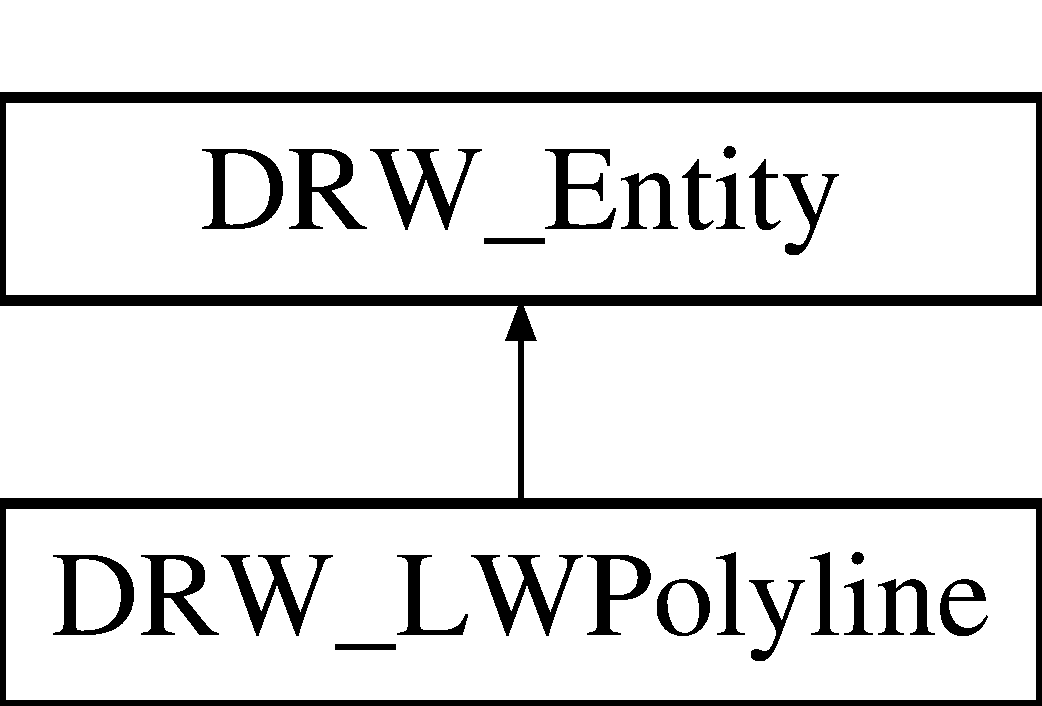
\includegraphics[height=2.000000cm]{d8/dc8/class_d_r_w___l_w_polyline}
\end{center}
\end{figure}
\subsection*{Public Attributes}
\begin{DoxyCompactItemize}
\item 
int \hyperlink{class_d_r_w___l_w_polyline_a7aa318239f9956b6e0331199491e20a5}{vertexnum}
\item 
int \hyperlink{class_d_r_w___l_w_polyline_a66f6b406675a3c4ef540099356973510}{flags}
\item 
double \hyperlink{class_d_r_w___l_w_polyline_aedd6dd732a0b425711921104b52f8ce9}{width}
\item 
double \hyperlink{class_d_r_w___l_w_polyline_a86ba4b8badb8f008997401ec9f084a3b}{elevation}
\item 
double \hyperlink{class_d_r_w___l_w_polyline_abab38cc3e874a5c89469b382ebeb2284}{thickness}
\item 
\hyperlink{class_d_r_w___coord}{D\+R\+W\+\_\+\+Coord} \hyperlink{class_d_r_w___l_w_polyline_a859105f0a27e812dc074483809a38194}{ext\+Point}
\item 
\hyperlink{class_d_r_w___vertex2_d}{D\+R\+W\+\_\+\+Vertex2\+D} $\ast$ \hyperlink{class_d_r_w___l_w_polyline_af59a2babb12d2f8865991c39cf464538}{vertex}
\item 
std\+::vector$<$ \hyperlink{class_d_r_w___vertex2_d}{D\+R\+W\+\_\+\+Vertex2\+D} $\ast$ $>$ \hyperlink{class_d_r_w___l_w_polyline_a2da7f3449eec6588fb3765a1c9541404}{vertlist}
\end{DoxyCompactItemize}
\subsection*{Additional Inherited Members}


\subsection{Detailed Description}
Class to handle lwpolyline entity. 

Class to handle lwpolyline entity \begin{DoxyAuthor}{Author}
Rallaz 
\end{DoxyAuthor}


\subsection{Member Data Documentation}
\hypertarget{class_d_r_w___l_w_polyline_a86ba4b8badb8f008997401ec9f084a3b}{}\index{D\+R\+W\+\_\+\+L\+W\+Polyline@{D\+R\+W\+\_\+\+L\+W\+Polyline}!elevation@{elevation}}
\index{elevation@{elevation}!D\+R\+W\+\_\+\+L\+W\+Polyline@{D\+R\+W\+\_\+\+L\+W\+Polyline}}
\subsubsection[{elevation}]{\setlength{\rightskip}{0pt plus 5cm}double D\+R\+W\+\_\+\+L\+W\+Polyline\+::elevation}\label{class_d_r_w___l_w_polyline_a86ba4b8badb8f008997401ec9f084a3b}
elevation, code 38 \hypertarget{class_d_r_w___l_w_polyline_a859105f0a27e812dc074483809a38194}{}\index{D\+R\+W\+\_\+\+L\+W\+Polyline@{D\+R\+W\+\_\+\+L\+W\+Polyline}!ext\+Point@{ext\+Point}}
\index{ext\+Point@{ext\+Point}!D\+R\+W\+\_\+\+L\+W\+Polyline@{D\+R\+W\+\_\+\+L\+W\+Polyline}}
\subsubsection[{ext\+Point}]{\setlength{\rightskip}{0pt plus 5cm}{\bf D\+R\+W\+\_\+\+Coord} D\+R\+W\+\_\+\+L\+W\+Polyline\+::ext\+Point}\label{class_d_r_w___l_w_polyline_a859105f0a27e812dc074483809a38194}
Dir extrusion normal vector, code 210, 220 \& 230 \hypertarget{class_d_r_w___l_w_polyline_a66f6b406675a3c4ef540099356973510}{}\index{D\+R\+W\+\_\+\+L\+W\+Polyline@{D\+R\+W\+\_\+\+L\+W\+Polyline}!flags@{flags}}
\index{flags@{flags}!D\+R\+W\+\_\+\+L\+W\+Polyline@{D\+R\+W\+\_\+\+L\+W\+Polyline}}
\subsubsection[{flags}]{\setlength{\rightskip}{0pt plus 5cm}int D\+R\+W\+\_\+\+L\+W\+Polyline\+::flags}\label{class_d_r_w___l_w_polyline_a66f6b406675a3c4ef540099356973510}
polyline flag, code 70, default 0 \hypertarget{class_d_r_w___l_w_polyline_abab38cc3e874a5c89469b382ebeb2284}{}\index{D\+R\+W\+\_\+\+L\+W\+Polyline@{D\+R\+W\+\_\+\+L\+W\+Polyline}!thickness@{thickness}}
\index{thickness@{thickness}!D\+R\+W\+\_\+\+L\+W\+Polyline@{D\+R\+W\+\_\+\+L\+W\+Polyline}}
\subsubsection[{thickness}]{\setlength{\rightskip}{0pt plus 5cm}double D\+R\+W\+\_\+\+L\+W\+Polyline\+::thickness}\label{class_d_r_w___l_w_polyline_abab38cc3e874a5c89469b382ebeb2284}
thickness, code 39 \hypertarget{class_d_r_w___l_w_polyline_af59a2babb12d2f8865991c39cf464538}{}\index{D\+R\+W\+\_\+\+L\+W\+Polyline@{D\+R\+W\+\_\+\+L\+W\+Polyline}!vertex@{vertex}}
\index{vertex@{vertex}!D\+R\+W\+\_\+\+L\+W\+Polyline@{D\+R\+W\+\_\+\+L\+W\+Polyline}}
\subsubsection[{vertex}]{\setlength{\rightskip}{0pt plus 5cm}{\bf D\+R\+W\+\_\+\+Vertex2\+D}$\ast$ D\+R\+W\+\_\+\+L\+W\+Polyline\+::vertex}\label{class_d_r_w___l_w_polyline_af59a2babb12d2f8865991c39cf464538}
current vertex to add data \hypertarget{class_d_r_w___l_w_polyline_a7aa318239f9956b6e0331199491e20a5}{}\index{D\+R\+W\+\_\+\+L\+W\+Polyline@{D\+R\+W\+\_\+\+L\+W\+Polyline}!vertexnum@{vertexnum}}
\index{vertexnum@{vertexnum}!D\+R\+W\+\_\+\+L\+W\+Polyline@{D\+R\+W\+\_\+\+L\+W\+Polyline}}
\subsubsection[{vertexnum}]{\setlength{\rightskip}{0pt plus 5cm}int D\+R\+W\+\_\+\+L\+W\+Polyline\+::vertexnum}\label{class_d_r_w___l_w_polyline_a7aa318239f9956b6e0331199491e20a5}
number of vertex, code 90 \hypertarget{class_d_r_w___l_w_polyline_a2da7f3449eec6588fb3765a1c9541404}{}\index{D\+R\+W\+\_\+\+L\+W\+Polyline@{D\+R\+W\+\_\+\+L\+W\+Polyline}!vertlist@{vertlist}}
\index{vertlist@{vertlist}!D\+R\+W\+\_\+\+L\+W\+Polyline@{D\+R\+W\+\_\+\+L\+W\+Polyline}}
\subsubsection[{vertlist}]{\setlength{\rightskip}{0pt plus 5cm}std\+::vector$<${\bf D\+R\+W\+\_\+\+Vertex2\+D} $\ast$$>$ D\+R\+W\+\_\+\+L\+W\+Polyline\+::vertlist}\label{class_d_r_w___l_w_polyline_a2da7f3449eec6588fb3765a1c9541404}
vertex list \hypertarget{class_d_r_w___l_w_polyline_aedd6dd732a0b425711921104b52f8ce9}{}\index{D\+R\+W\+\_\+\+L\+W\+Polyline@{D\+R\+W\+\_\+\+L\+W\+Polyline}!width@{width}}
\index{width@{width}!D\+R\+W\+\_\+\+L\+W\+Polyline@{D\+R\+W\+\_\+\+L\+W\+Polyline}}
\subsubsection[{width}]{\setlength{\rightskip}{0pt plus 5cm}double D\+R\+W\+\_\+\+L\+W\+Polyline\+::width}\label{class_d_r_w___l_w_polyline_aedd6dd732a0b425711921104b52f8ce9}
constant width, code 43 

The documentation for this class was generated from the following files\+:\begin{DoxyCompactItemize}
\item 
src/drw\+\_\+entities.\+h\item 
src/drw\+\_\+entities.\+cpp\end{DoxyCompactItemize}

\hypertarget{class_d_r_w___m_text}{}\section{D\+R\+W\+\_\+\+M\+Text Class Reference}
\label{class_d_r_w___m_text}\index{D\+R\+W\+\_\+\+M\+Text@{D\+R\+W\+\_\+\+M\+Text}}


Class to handle insert entries.  




{\ttfamily \#include $<$drw\+\_\+entities.\+h$>$}

Inheritance diagram for D\+R\+W\+\_\+\+M\+Text\+:\begin{figure}[H]
\begin{center}
\leavevmode
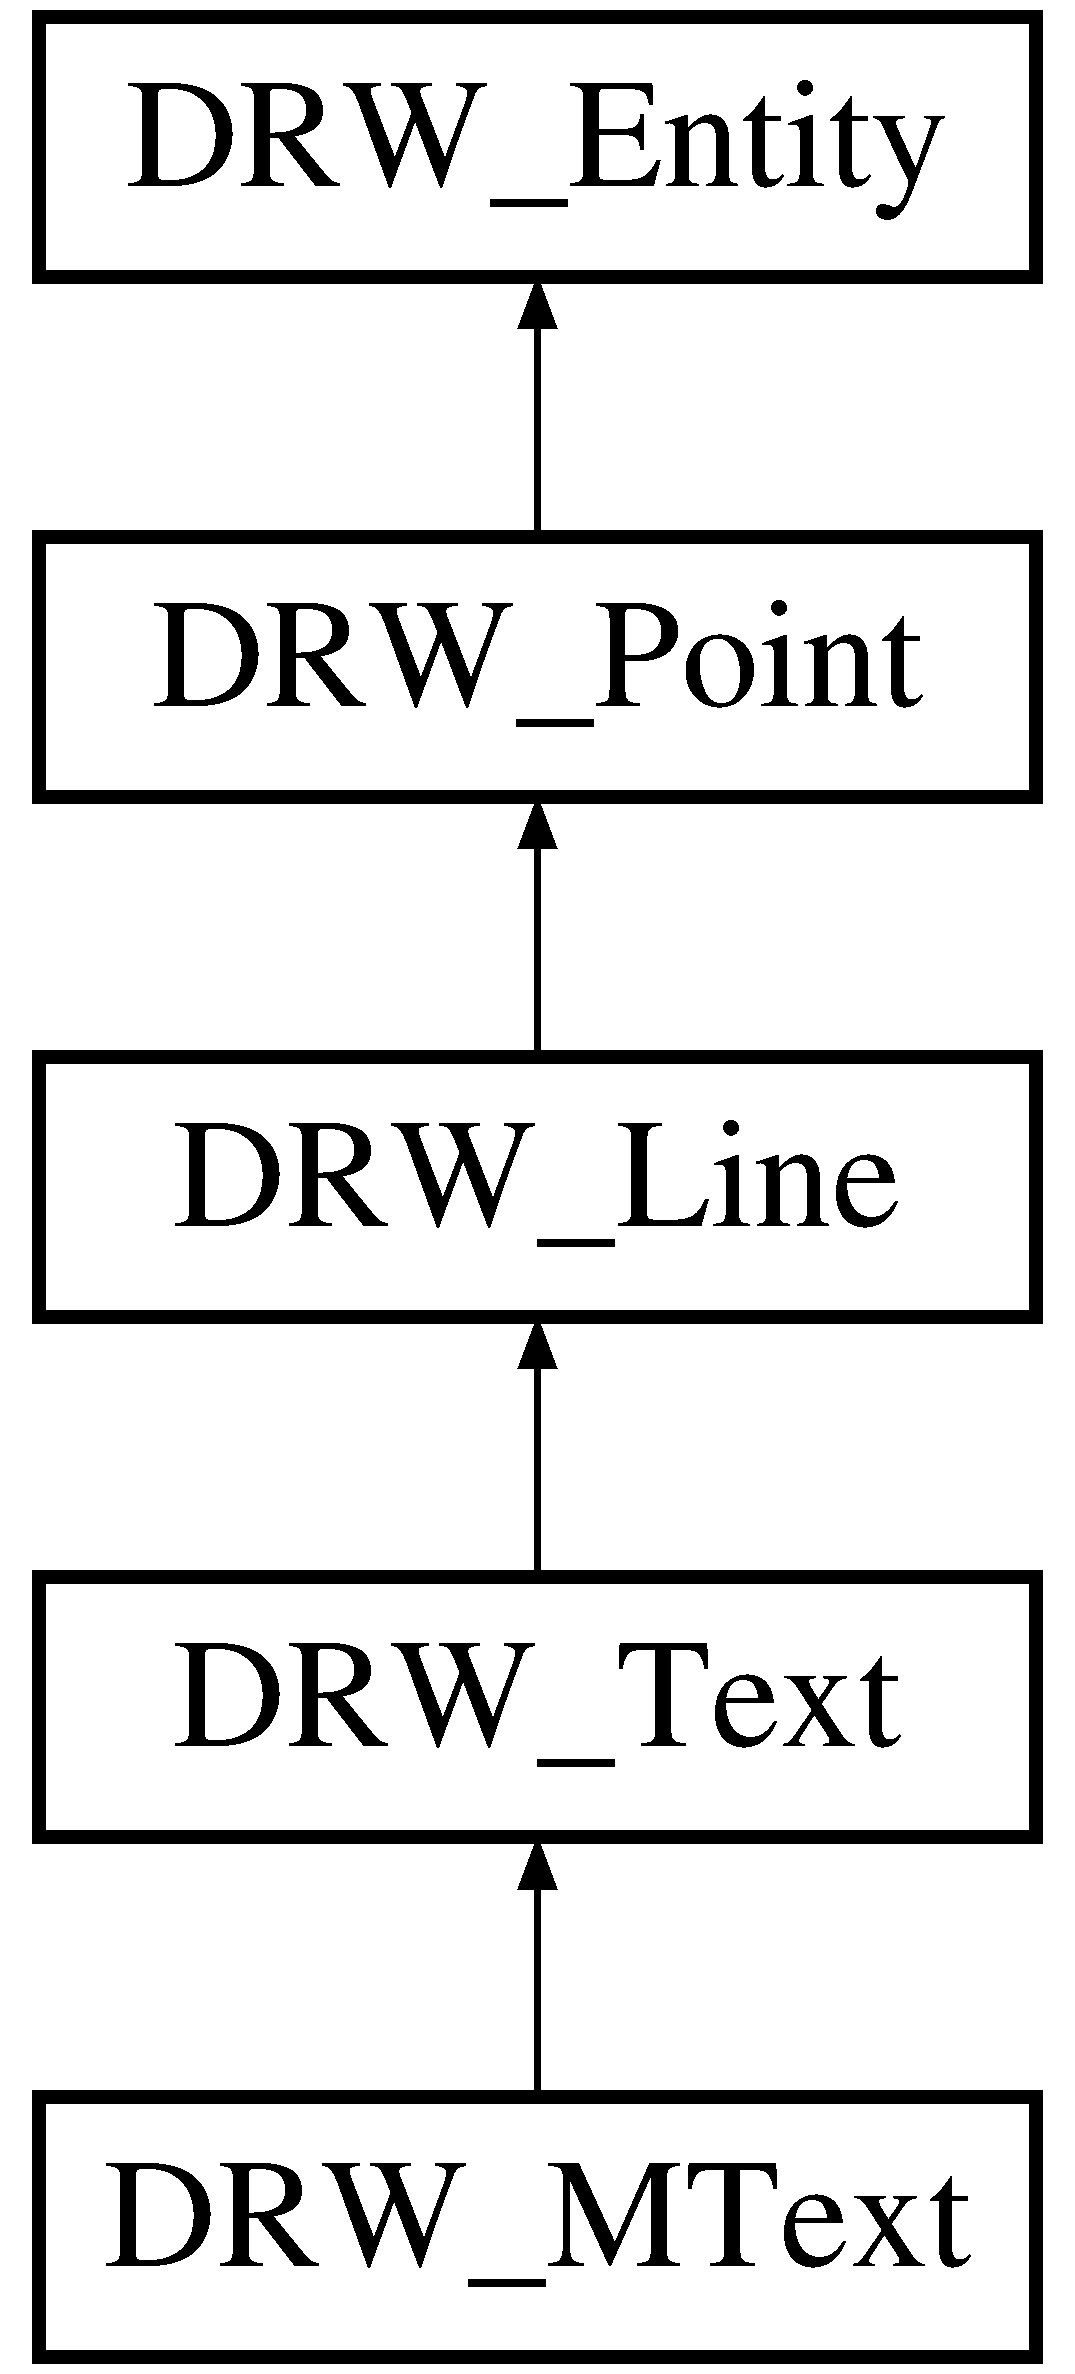
\includegraphics[height=5.000000cm]{d3/d1a/class_d_r_w___m_text}
\end{center}
\end{figure}
\subsection*{Public Types}
\begin{DoxyCompactItemize}
\item 
\hypertarget{class_d_r_w___m_text_a19eb89e577ee3e259f52bc7aebf7b84c}{}enum \hyperlink{class_d_r_w___m_text_a19eb89e577ee3e259f52bc7aebf7b84c}{Attach} \label{class_d_r_w___m_text_a19eb89e577ee3e259f52bc7aebf7b84c}

\begin{DoxyCompactList}\small\item\em Attachments. \end{DoxyCompactList}\end{DoxyCompactItemize}
\subsection*{Public Attributes}
\begin{DoxyCompactItemize}
\item 
double \hyperlink{class_d_r_w___m_text_a60c7259ea36123406c5270dcd5434efa}{interlin}
\end{DoxyCompactItemize}
\subsection*{Protected Member Functions}
\begin{DoxyCompactItemize}
\item 
virtual bool \hyperlink{class_d_r_w___m_text_a907a02526a50cef1f93487dbf8b929b8}{parse\+Dwg} (D\+R\+W\+::\+Version version, dwg\+Buffer $\ast$buf)
\end{DoxyCompactItemize}


\subsection{Detailed Description}
Class to handle insert entries. 

Class to handle insert entries \begin{DoxyAuthor}{Author}
Rallaz 
\end{DoxyAuthor}


\subsection{Member Function Documentation}
\hypertarget{class_d_r_w___m_text_a907a02526a50cef1f93487dbf8b929b8}{}\index{D\+R\+W\+\_\+\+M\+Text@{D\+R\+W\+\_\+\+M\+Text}!parse\+Dwg@{parse\+Dwg}}
\index{parse\+Dwg@{parse\+Dwg}!D\+R\+W\+\_\+\+M\+Text@{D\+R\+W\+\_\+\+M\+Text}}
\subsubsection[{parse\+Dwg}]{\setlength{\rightskip}{0pt plus 5cm}bool D\+R\+W\+\_\+\+M\+Text\+::parse\+Dwg (
\begin{DoxyParamCaption}
\item[{D\+R\+W\+::\+Version}]{version, }
\item[{dwg\+Buffer $\ast$}]{buf}
\end{DoxyParamCaption}
)\hspace{0.3cm}{\ttfamily [protected]}, {\ttfamily [virtual]}}\label{class_d_r_w___m_text_a907a02526a50cef1f93487dbf8b929b8}
\begin{DoxyRefDesc}{Todo}
\item[\hyperlink{todo__todo000001}{Todo}]compute the angle from this \end{DoxyRefDesc}


\begin{DoxyRefDesc}{Todo}
\item[\hyperlink{todo__todo000002}{Todo}]\end{DoxyRefDesc}


\begin{DoxyRefDesc}{Todo}
\item[\hyperlink{todo__todo000003}{Todo}]add to \hyperlink{class_d_r_w___m_text}{D\+R\+W\+\_\+\+M\+Text} \end{DoxyRefDesc}


\begin{DoxyRefDesc}{Todo}
\item[\hyperlink{todo__todo000004}{Todo}]buf-\/$>$get\+C\+M\+C \end{DoxyRefDesc}


Reimplemented from \hyperlink{class_d_r_w___text}{D\+R\+W\+\_\+\+Text}.



\subsection{Member Data Documentation}
\hypertarget{class_d_r_w___m_text_a60c7259ea36123406c5270dcd5434efa}{}\index{D\+R\+W\+\_\+\+M\+Text@{D\+R\+W\+\_\+\+M\+Text}!interlin@{interlin}}
\index{interlin@{interlin}!D\+R\+W\+\_\+\+M\+Text@{D\+R\+W\+\_\+\+M\+Text}}
\subsubsection[{interlin}]{\setlength{\rightskip}{0pt plus 5cm}double D\+R\+W\+\_\+\+M\+Text\+::interlin}\label{class_d_r_w___m_text_a60c7259ea36123406c5270dcd5434efa}
width factor, code 44 

The documentation for this class was generated from the following files\+:\begin{DoxyCompactItemize}
\item 
src/drw\+\_\+entities.\+h\item 
src/drw\+\_\+entities.\+cpp\end{DoxyCompactItemize}

\hypertarget{class_d_r_w___point}{}\section{D\+R\+W\+\_\+\+Point Class Reference}
\label{class_d_r_w___point}\index{D\+R\+W\+\_\+\+Point@{D\+R\+W\+\_\+\+Point}}


Class to handle point entity.  




{\ttfamily \#include $<$drw\+\_\+entities.\+h$>$}

Inheritance diagram for D\+R\+W\+\_\+\+Point\+:\begin{figure}[H]
\begin{center}
\leavevmode
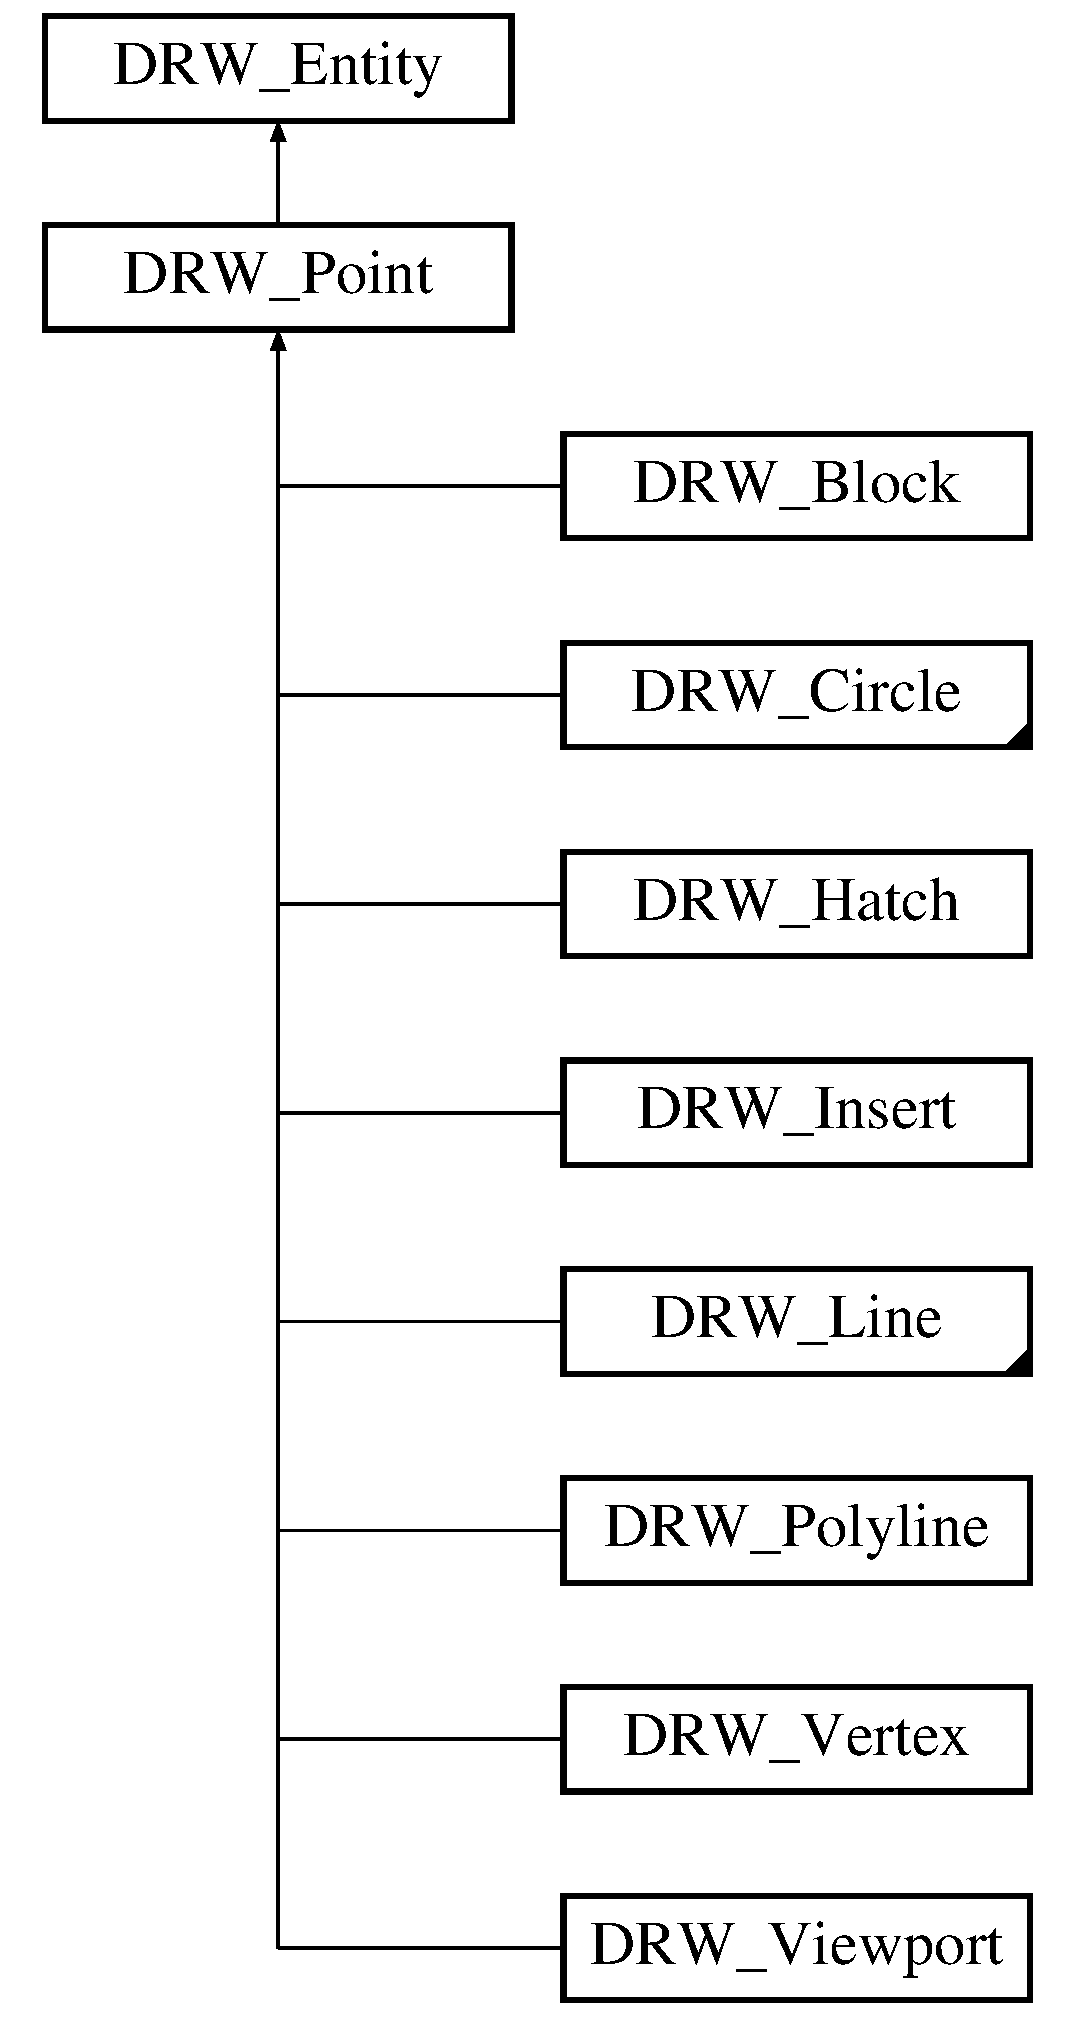
\includegraphics[height=10.000000cm]{d9/d53/class_d_r_w___point}
\end{center}
\end{figure}
\subsection*{Public Attributes}
\begin{DoxyCompactItemize}
\item 
\hyperlink{class_d_r_w___coord}{D\+R\+W\+\_\+\+Coord} \hyperlink{class_d_r_w___point_afaa15dc45c45d9057257e478c9746169}{base\+Point}
\item 
double \hyperlink{class_d_r_w___point_a909f6f2623e3b5cf40393636f3119954}{thickness}
\item 
\hyperlink{class_d_r_w___coord}{D\+R\+W\+\_\+\+Coord} \hyperlink{class_d_r_w___point_ab55e32170a648e8469844c886ff56fc7}{ext\+Point}
\end{DoxyCompactItemize}
\subsection*{Additional Inherited Members}


\subsection{Detailed Description}
Class to handle point entity. 

Class to handle point entity \begin{DoxyAuthor}{Author}
Rallaz 
\end{DoxyAuthor}


\subsection{Member Data Documentation}
\hypertarget{class_d_r_w___point_afaa15dc45c45d9057257e478c9746169}{}\index{D\+R\+W\+\_\+\+Point@{D\+R\+W\+\_\+\+Point}!base\+Point@{base\+Point}}
\index{base\+Point@{base\+Point}!D\+R\+W\+\_\+\+Point@{D\+R\+W\+\_\+\+Point}}
\subsubsection[{base\+Point}]{\setlength{\rightskip}{0pt plus 5cm}{\bf D\+R\+W\+\_\+\+Coord} D\+R\+W\+\_\+\+Point\+::base\+Point}\label{class_d_r_w___point_afaa15dc45c45d9057257e478c9746169}
base point, code 10, 20 \& 30 \hypertarget{class_d_r_w___point_ab55e32170a648e8469844c886ff56fc7}{}\index{D\+R\+W\+\_\+\+Point@{D\+R\+W\+\_\+\+Point}!ext\+Point@{ext\+Point}}
\index{ext\+Point@{ext\+Point}!D\+R\+W\+\_\+\+Point@{D\+R\+W\+\_\+\+Point}}
\subsubsection[{ext\+Point}]{\setlength{\rightskip}{0pt plus 5cm}{\bf D\+R\+W\+\_\+\+Coord} D\+R\+W\+\_\+\+Point\+::ext\+Point}\label{class_d_r_w___point_ab55e32170a648e8469844c886ff56fc7}
Dir extrusion normal vector, code 210, 220 \& 230 \hypertarget{class_d_r_w___point_a909f6f2623e3b5cf40393636f3119954}{}\index{D\+R\+W\+\_\+\+Point@{D\+R\+W\+\_\+\+Point}!thickness@{thickness}}
\index{thickness@{thickness}!D\+R\+W\+\_\+\+Point@{D\+R\+W\+\_\+\+Point}}
\subsubsection[{thickness}]{\setlength{\rightskip}{0pt plus 5cm}double D\+R\+W\+\_\+\+Point\+::thickness}\label{class_d_r_w___point_a909f6f2623e3b5cf40393636f3119954}
thickness, code 39 

The documentation for this class was generated from the following files\+:\begin{DoxyCompactItemize}
\item 
src/drw\+\_\+entities.\+h\item 
src/drw\+\_\+entities.\+cpp\end{DoxyCompactItemize}

\hypertarget{class_d_r_w___polyline}{}\section{D\+R\+W\+\_\+\+Polyline Class Reference}
\label{class_d_r_w___polyline}\index{D\+R\+W\+\_\+\+Polyline@{D\+R\+W\+\_\+\+Polyline}}


Class to handle polyline entity.  




{\ttfamily \#include $<$drw\+\_\+entities.\+h$>$}

Inheritance diagram for D\+R\+W\+\_\+\+Polyline\+:\begin{figure}[H]
\begin{center}
\leavevmode
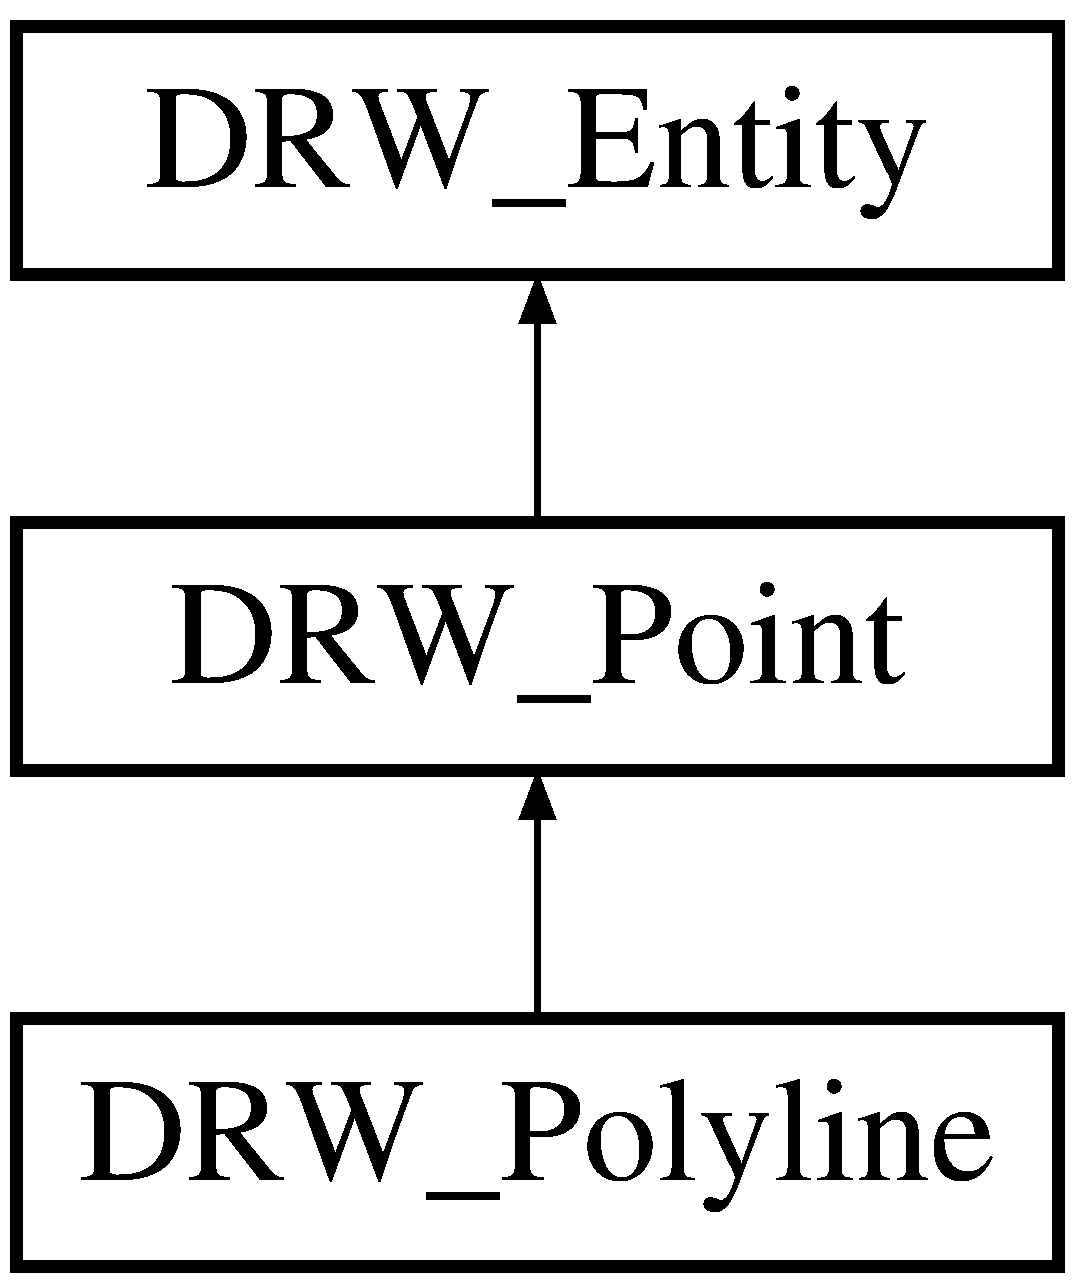
\includegraphics[height=3.000000cm]{d2/dc3/class_d_r_w___polyline}
\end{center}
\end{figure}
\subsection*{Public Attributes}
\begin{DoxyCompactItemize}
\item 
int \hyperlink{class_d_r_w___polyline_a328f232ca859ae9f5561e78457833099}{flags}
\item 
double \hyperlink{class_d_r_w___polyline_a47b35f26221533fdd0d7ef2d91925ca3}{defstawidth}
\item 
double \hyperlink{class_d_r_w___polyline_a8818ce849a6704cb7d83ba7792f3db50}{defendwidth}
\item 
int \hyperlink{class_d_r_w___polyline_ac4bec6f33dd2f8967548d7163525537e}{vertexcount}
\item 
int \hyperlink{class_d_r_w___polyline_ae7e68c83478c4dad5550cfc44fa524bd}{facecount}
\item 
int \hyperlink{class_d_r_w___polyline_aa244ad2243bc7312e01b39876da95edb}{smooth\+M}
\item 
int \hyperlink{class_d_r_w___polyline_a35895911a129d179e1197efa9ca0ec34}{smooth\+N}
\item 
int \hyperlink{class_d_r_w___polyline_a9cd44431960f6b199c218da6ca475fdb}{curvetype}
\item 
std\+::vector$<$ \hyperlink{class_d_r_w___vertex}{D\+R\+W\+\_\+\+Vertex} $\ast$ $>$ \hyperlink{class_d_r_w___polyline_ab001a6b7d6fec6298f52cc1f47df6c87}{vertlist}
\end{DoxyCompactItemize}
\subsection*{Friends}
\begin{DoxyCompactItemize}
\item 
\hypertarget{class_d_r_w___polyline_a7f080e77e5112f8364c61b97387f8ee2}{}class {\bfseries dxf\+R\+W}\label{class_d_r_w___polyline_a7f080e77e5112f8364c61b97387f8ee2}

\end{DoxyCompactItemize}
\subsection*{Additional Inherited Members}


\subsection{Detailed Description}
Class to handle polyline entity. 

Class to handle polyline entity \begin{DoxyAuthor}{Author}
Rallaz 
\end{DoxyAuthor}


\subsection{Member Data Documentation}
\hypertarget{class_d_r_w___polyline_a9cd44431960f6b199c218da6ca475fdb}{}\index{D\+R\+W\+\_\+\+Polyline@{D\+R\+W\+\_\+\+Polyline}!curvetype@{curvetype}}
\index{curvetype@{curvetype}!D\+R\+W\+\_\+\+Polyline@{D\+R\+W\+\_\+\+Polyline}}
\subsubsection[{curvetype}]{\setlength{\rightskip}{0pt plus 5cm}int D\+R\+W\+\_\+\+Polyline\+::curvetype}\label{class_d_r_w___polyline_a9cd44431960f6b199c218da6ca475fdb}
curves \& smooth surface type, code 75, default 0 \hypertarget{class_d_r_w___polyline_a8818ce849a6704cb7d83ba7792f3db50}{}\index{D\+R\+W\+\_\+\+Polyline@{D\+R\+W\+\_\+\+Polyline}!defendwidth@{defendwidth}}
\index{defendwidth@{defendwidth}!D\+R\+W\+\_\+\+Polyline@{D\+R\+W\+\_\+\+Polyline}}
\subsubsection[{defendwidth}]{\setlength{\rightskip}{0pt plus 5cm}double D\+R\+W\+\_\+\+Polyline\+::defendwidth}\label{class_d_r_w___polyline_a8818ce849a6704cb7d83ba7792f3db50}
End width, code 41, default 0 \hypertarget{class_d_r_w___polyline_a47b35f26221533fdd0d7ef2d91925ca3}{}\index{D\+R\+W\+\_\+\+Polyline@{D\+R\+W\+\_\+\+Polyline}!defstawidth@{defstawidth}}
\index{defstawidth@{defstawidth}!D\+R\+W\+\_\+\+Polyline@{D\+R\+W\+\_\+\+Polyline}}
\subsubsection[{defstawidth}]{\setlength{\rightskip}{0pt plus 5cm}double D\+R\+W\+\_\+\+Polyline\+::defstawidth}\label{class_d_r_w___polyline_a47b35f26221533fdd0d7ef2d91925ca3}
Start width, code 40, default 0 \hypertarget{class_d_r_w___polyline_ae7e68c83478c4dad5550cfc44fa524bd}{}\index{D\+R\+W\+\_\+\+Polyline@{D\+R\+W\+\_\+\+Polyline}!facecount@{facecount}}
\index{facecount@{facecount}!D\+R\+W\+\_\+\+Polyline@{D\+R\+W\+\_\+\+Polyline}}
\subsubsection[{facecount}]{\setlength{\rightskip}{0pt plus 5cm}int D\+R\+W\+\_\+\+Polyline\+::facecount}\label{class_d_r_w___polyline_ae7e68c83478c4dad5550cfc44fa524bd}
polygon mesh N vertex or polyface face num, code 72, default 0 \hypertarget{class_d_r_w___polyline_a328f232ca859ae9f5561e78457833099}{}\index{D\+R\+W\+\_\+\+Polyline@{D\+R\+W\+\_\+\+Polyline}!flags@{flags}}
\index{flags@{flags}!D\+R\+W\+\_\+\+Polyline@{D\+R\+W\+\_\+\+Polyline}}
\subsubsection[{flags}]{\setlength{\rightskip}{0pt plus 5cm}int D\+R\+W\+\_\+\+Polyline\+::flags}\label{class_d_r_w___polyline_a328f232ca859ae9f5561e78457833099}
polyline flag, code 70, default 0 \hypertarget{class_d_r_w___polyline_aa244ad2243bc7312e01b39876da95edb}{}\index{D\+R\+W\+\_\+\+Polyline@{D\+R\+W\+\_\+\+Polyline}!smooth\+M@{smooth\+M}}
\index{smooth\+M@{smooth\+M}!D\+R\+W\+\_\+\+Polyline@{D\+R\+W\+\_\+\+Polyline}}
\subsubsection[{smooth\+M}]{\setlength{\rightskip}{0pt plus 5cm}int D\+R\+W\+\_\+\+Polyline\+::smooth\+M}\label{class_d_r_w___polyline_aa244ad2243bc7312e01b39876da95edb}
smooth surface M density, code 73, default 0 \hypertarget{class_d_r_w___polyline_a35895911a129d179e1197efa9ca0ec34}{}\index{D\+R\+W\+\_\+\+Polyline@{D\+R\+W\+\_\+\+Polyline}!smooth\+N@{smooth\+N}}
\index{smooth\+N@{smooth\+N}!D\+R\+W\+\_\+\+Polyline@{D\+R\+W\+\_\+\+Polyline}}
\subsubsection[{smooth\+N}]{\setlength{\rightskip}{0pt plus 5cm}int D\+R\+W\+\_\+\+Polyline\+::smooth\+N}\label{class_d_r_w___polyline_a35895911a129d179e1197efa9ca0ec34}
smooth surface M density, code 74, default 0 \hypertarget{class_d_r_w___polyline_ac4bec6f33dd2f8967548d7163525537e}{}\index{D\+R\+W\+\_\+\+Polyline@{D\+R\+W\+\_\+\+Polyline}!vertexcount@{vertexcount}}
\index{vertexcount@{vertexcount}!D\+R\+W\+\_\+\+Polyline@{D\+R\+W\+\_\+\+Polyline}}
\subsubsection[{vertexcount}]{\setlength{\rightskip}{0pt plus 5cm}int D\+R\+W\+\_\+\+Polyline\+::vertexcount}\label{class_d_r_w___polyline_ac4bec6f33dd2f8967548d7163525537e}
polygon mesh M vertex or polyface vertex num, code 71, default 0 \hypertarget{class_d_r_w___polyline_ab001a6b7d6fec6298f52cc1f47df6c87}{}\index{D\+R\+W\+\_\+\+Polyline@{D\+R\+W\+\_\+\+Polyline}!vertlist@{vertlist}}
\index{vertlist@{vertlist}!D\+R\+W\+\_\+\+Polyline@{D\+R\+W\+\_\+\+Polyline}}
\subsubsection[{vertlist}]{\setlength{\rightskip}{0pt plus 5cm}std\+::vector$<${\bf D\+R\+W\+\_\+\+Vertex} $\ast$$>$ D\+R\+W\+\_\+\+Polyline\+::vertlist}\label{class_d_r_w___polyline_ab001a6b7d6fec6298f52cc1f47df6c87}
vertex list 

The documentation for this class was generated from the following files\+:\begin{DoxyCompactItemize}
\item 
src/drw\+\_\+entities.\+h\item 
src/drw\+\_\+entities.\+cpp\end{DoxyCompactItemize}

\hypertarget{class_d_r_w___ray}{}\section{D\+R\+W\+\_\+\+Ray Class Reference}
\label{class_d_r_w___ray}\index{D\+R\+W\+\_\+\+Ray@{D\+R\+W\+\_\+\+Ray}}


Class to handle ray entity.  




{\ttfamily \#include $<$drw\+\_\+entities.\+h$>$}

Inheritance diagram for D\+R\+W\+\_\+\+Ray\+:\begin{figure}[H]
\begin{center}
\leavevmode
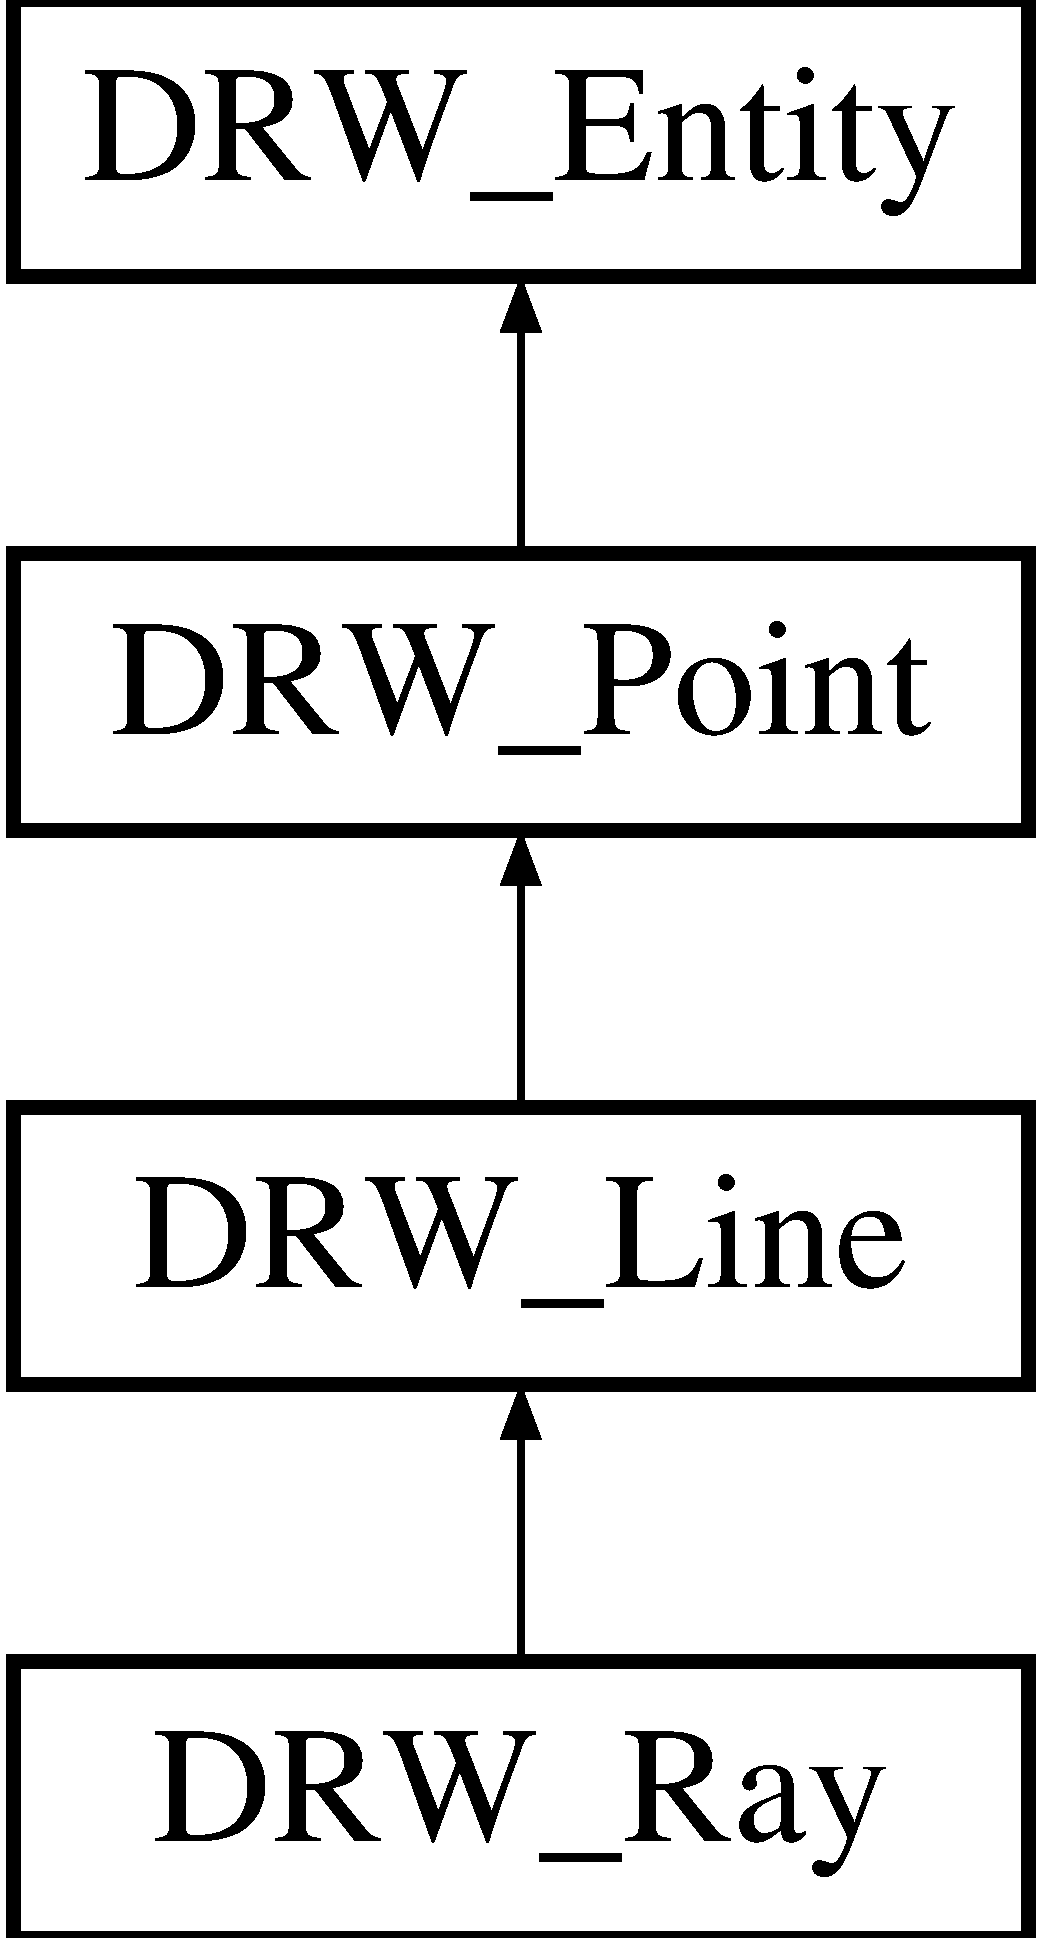
\includegraphics[height=4.000000cm]{dc/df9/class_d_r_w___ray}
\end{center}
\end{figure}
\subsection*{Additional Inherited Members}


\subsection{Detailed Description}
Class to handle ray entity. 

Class to handle ray entity \begin{DoxyAuthor}{Author}
Rallaz 
\end{DoxyAuthor}


The documentation for this class was generated from the following file\+:\begin{DoxyCompactItemize}
\item 
src/drw\+\_\+entities.\+h\end{DoxyCompactItemize}

\hypertarget{class_d_r_w___solid}{}\section{D\+R\+W\+\_\+\+Solid Class Reference}
\label{class_d_r_w___solid}\index{D\+R\+W\+\_\+\+Solid@{D\+R\+W\+\_\+\+Solid}}


Class to handle solid entity.  




{\ttfamily \#include $<$drw\+\_\+entities.\+h$>$}

Inheritance diagram for D\+R\+W\+\_\+\+Solid\+:\begin{figure}[H]
\begin{center}
\leavevmode
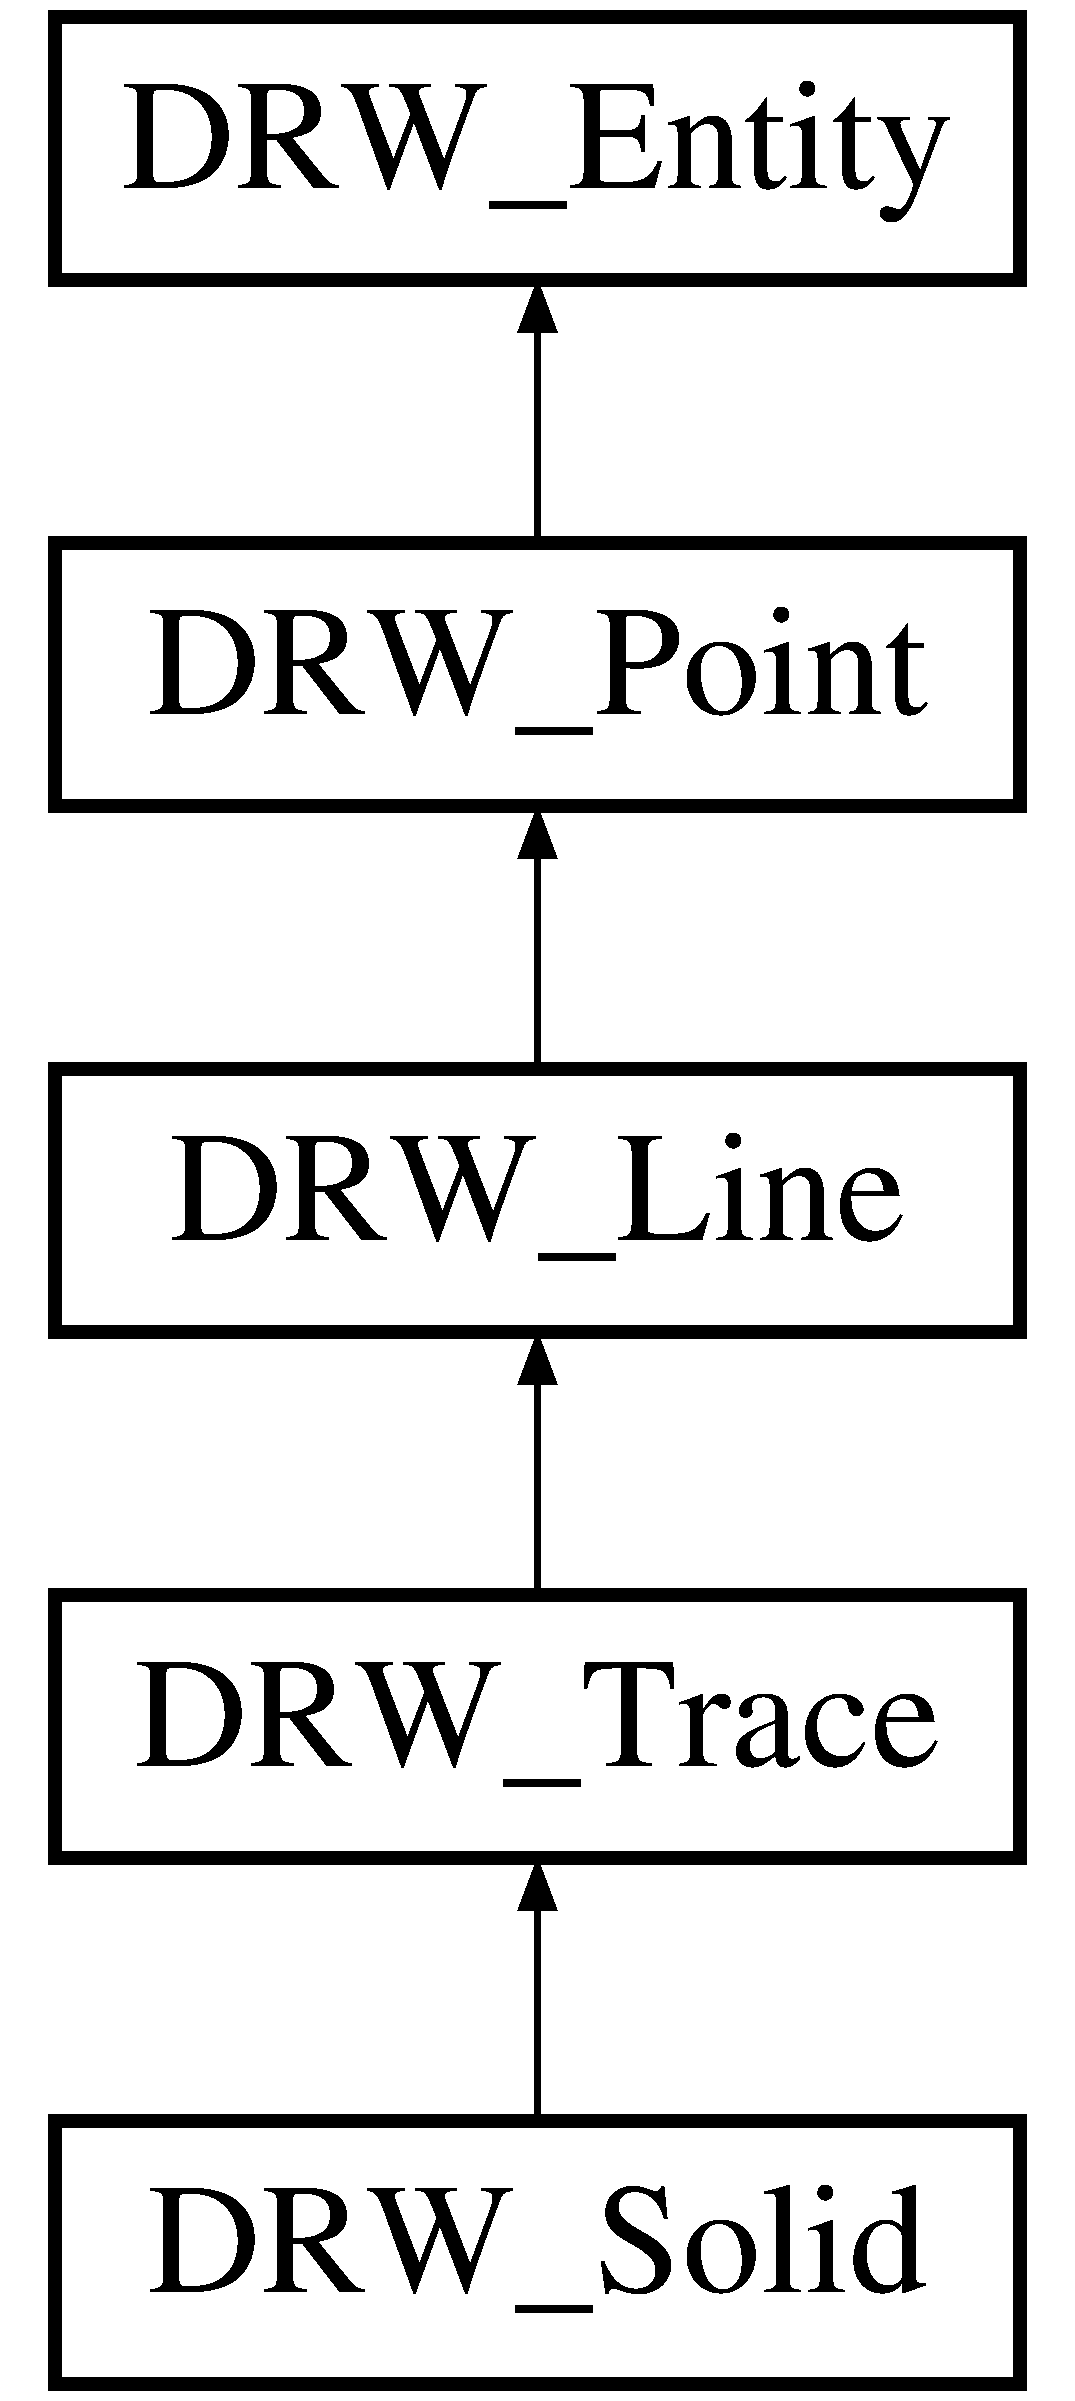
\includegraphics[height=5.000000cm]{d6/dc1/class_d_r_w___solid}
\end{center}
\end{figure}
\subsection*{Public Member Functions}
\begin{DoxyCompactItemize}
\item 
\hypertarget{class_d_r_w___solid_aceafc144bdb6f9debde7ef5220d527de}{}const \hyperlink{class_d_r_w___coord}{D\+R\+W\+\_\+\+Coord} \& \hyperlink{class_d_r_w___solid_aceafc144bdb6f9debde7ef5220d527de}{first\+Corner} ()\label{class_d_r_w___solid_aceafc144bdb6f9debde7ef5220d527de}

\begin{DoxyCompactList}\small\item\em first corner (2\+D) \end{DoxyCompactList}\item 
\hypertarget{class_d_r_w___solid_aa0122aff6219b5e49036aecd8da2857f}{}const \hyperlink{class_d_r_w___coord}{D\+R\+W\+\_\+\+Coord} \& \hyperlink{class_d_r_w___solid_aa0122aff6219b5e49036aecd8da2857f}{second\+Corner} ()\label{class_d_r_w___solid_aa0122aff6219b5e49036aecd8da2857f}

\begin{DoxyCompactList}\small\item\em second corner (2\+D) \end{DoxyCompactList}\item 
\hypertarget{class_d_r_w___solid_a54fa47c874ff49996fe94fb8c046f9dd}{}const \hyperlink{class_d_r_w___coord}{D\+R\+W\+\_\+\+Coord} \& \hyperlink{class_d_r_w___solid_a54fa47c874ff49996fe94fb8c046f9dd}{third\+Corner} ()\label{class_d_r_w___solid_a54fa47c874ff49996fe94fb8c046f9dd}

\begin{DoxyCompactList}\small\item\em third corner (2\+D) \end{DoxyCompactList}\item 
\hypertarget{class_d_r_w___solid_a22c02304f0275e38e29b2744681e3571}{}const \hyperlink{class_d_r_w___coord}{D\+R\+W\+\_\+\+Coord} \& \hyperlink{class_d_r_w___solid_a22c02304f0275e38e29b2744681e3571}{fourth\+Corner} ()\label{class_d_r_w___solid_a22c02304f0275e38e29b2744681e3571}

\begin{DoxyCompactList}\small\item\em fourth corner (2\+D) \end{DoxyCompactList}\item 
\hypertarget{class_d_r_w___solid_a1ab7f7398cddbded52c299f82daca0bf}{}double \hyperlink{class_d_r_w___solid_a1ab7f7398cddbded52c299f82daca0bf}{thick} ()\label{class_d_r_w___solid_a1ab7f7398cddbded52c299f82daca0bf}

\begin{DoxyCompactList}\small\item\em thickness \end{DoxyCompactList}\item 
\hypertarget{class_d_r_w___solid_a38342cb41e9b3aeae1fe4f709c2558e8}{}double \hyperlink{class_d_r_w___solid_a38342cb41e9b3aeae1fe4f709c2558e8}{elevation} ()\label{class_d_r_w___solid_a38342cb41e9b3aeae1fe4f709c2558e8}

\begin{DoxyCompactList}\small\item\em elevation \end{DoxyCompactList}\item 
\hypertarget{class_d_r_w___solid_aaff3bcd0e5bb8927bc4748acc23019a4}{}const \hyperlink{class_d_r_w___coord}{D\+R\+W\+\_\+\+Coord} \& \hyperlink{class_d_r_w___solid_aaff3bcd0e5bb8927bc4748acc23019a4}{extrusion} ()\label{class_d_r_w___solid_aaff3bcd0e5bb8927bc4748acc23019a4}

\begin{DoxyCompactList}\small\item\em extrusion \end{DoxyCompactList}\end{DoxyCompactItemize}
\subsection*{Protected Member Functions}
\begin{DoxyCompactItemize}
\item 
\hypertarget{class_d_r_w___solid_a6afdf664e6245381382d2646d52d0638}{}void \hyperlink{class_d_r_w___solid_a6afdf664e6245381382d2646d52d0638}{parse\+Code} (int code, dxf\+Reader $\ast$reader)\label{class_d_r_w___solid_a6afdf664e6245381382d2646d52d0638}

\begin{DoxyCompactList}\small\item\em interpret code in dxf reading process or dispatch to inherited class \end{DoxyCompactList}\item 
\hypertarget{class_d_r_w___solid_a7d87f532461cd372336ba8d16976b0f4}{}virtual bool \hyperlink{class_d_r_w___solid_a7d87f532461cd372336ba8d16976b0f4}{parse\+Dwg} (D\+R\+W\+::\+Version v, dwg\+Buffer $\ast$buf)\label{class_d_r_w___solid_a7d87f532461cd372336ba8d16976b0f4}

\begin{DoxyCompactList}\small\item\em interpret dwg data (was already determined to be part of this object) \end{DoxyCompactList}\end{DoxyCompactItemize}
\subsection*{Additional Inherited Members}


\subsection{Detailed Description}
Class to handle solid entity. 

Class to handle solid entity \begin{DoxyAuthor}{Author}
Rallaz 
\end{DoxyAuthor}


The documentation for this class was generated from the following files\+:\begin{DoxyCompactItemize}
\item 
src/drw\+\_\+entities.\+h\item 
src/drw\+\_\+entities.\+cpp\end{DoxyCompactItemize}

\hypertarget{class_d_r_w___spline}{}\section{D\+R\+W\+\_\+\+Spline Class Reference}
\label{class_d_r_w___spline}\index{D\+R\+W\+\_\+\+Spline@{D\+R\+W\+\_\+\+Spline}}


Class to handle spline entity.  




{\ttfamily \#include $<$drw\+\_\+entities.\+h$>$}

Inheritance diagram for D\+R\+W\+\_\+\+Spline\+:\begin{figure}[H]
\begin{center}
\leavevmode
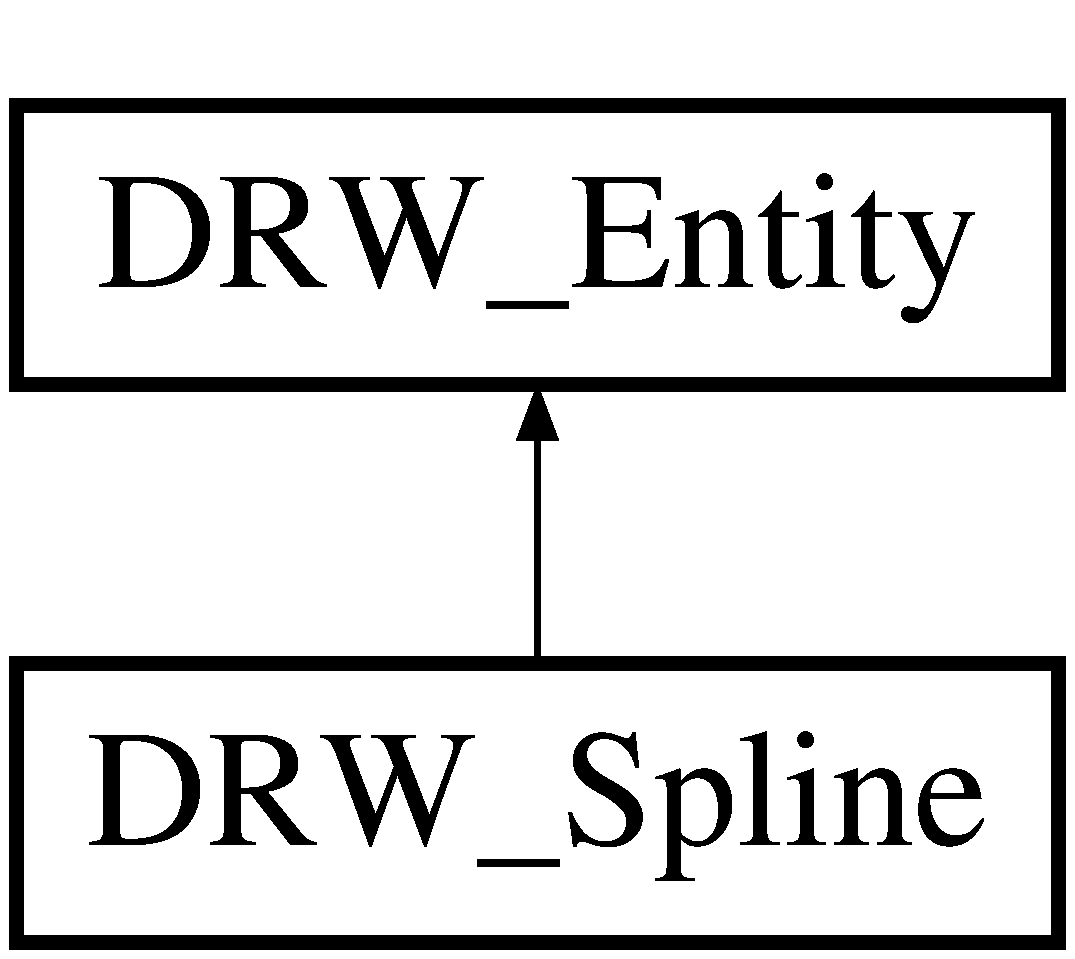
\includegraphics[height=2.000000cm]{d4/d9c/class_d_r_w___spline}
\end{center}
\end{figure}
\subsection*{Public Attributes}
\begin{DoxyCompactItemize}
\item 
double \hyperlink{class_d_r_w___spline_a7d2455d56e3de91a85a7afd1a5b34dfe}{ex}
\item 
double \hyperlink{class_d_r_w___spline_a937a3c0c4450e383de5ebbbbc892d1ad}{ey}
\item 
double \hyperlink{class_d_r_w___spline_ad3ad8a265fbc8c07bc06f8939a8a31a6}{ez}
\item 
double \hyperlink{class_d_r_w___spline_af669678833d9334001f372ef3e459063}{tgsx}
\item 
double \hyperlink{class_d_r_w___spline_a0d22ecfcfa1ccdf83d3799555b808fb6}{tgsy}
\item 
double \hyperlink{class_d_r_w___spline_a432ab2ee17f00fe8c3537f3ab12f0524}{tgsz}
\item 
double \hyperlink{class_d_r_w___spline_ae6195201183d629d458d820417587197}{tgex}
\item 
double \hyperlink{class_d_r_w___spline_a5bbb13c6219350335c353b86755adcea}{tgey}
\item 
double \hyperlink{class_d_r_w___spline_acfe280748cc843881dffd17430a2be37}{tgez}
\item 
int \hyperlink{class_d_r_w___spline_a49110f44d95d47090449c56beaaac3ca}{flags}
\item 
int \hyperlink{class_d_r_w___spline_af60e9efc3c39f418196cca4cc9f8125b}{degree}
\item 
int \hyperlink{class_d_r_w___spline_a5dd173d8176de55d07f00d96dedb0201}{nknots}
\item 
int \hyperlink{class_d_r_w___spline_a73dcf2fa67f1029e4a8d6577b5b51656}{ncontrol}
\item 
int \hyperlink{class_d_r_w___spline_aa9269fcfa581a0e0b25a84fb8dddc96c}{nfit}
\item 
double \hyperlink{class_d_r_w___spline_a62139497f4127ed0d909cbe6cb7d5304}{tolknot}
\item 
double \hyperlink{class_d_r_w___spline_a9ebcea64002b14f0adfae66eadd9f24a}{tolcontrol}
\item 
double \hyperlink{class_d_r_w___spline_a8f91c72942350988a2c3b4652162d613}{tolfit}
\item 
std\+::vector$<$ double $>$ \hyperlink{class_d_r_w___spline_a90bf2f53cd19d98629e393f3cdd36c95}{knotslist}
\item 
std\+::vector$<$ \hyperlink{class_d_r_w___coord}{D\+R\+W\+\_\+\+Coord} $\ast$ $>$ \hyperlink{class_d_r_w___spline_a37b5e6ce7e32c1577fed59c3704c0e0f}{controllist}
\item 
std\+::vector$<$ \hyperlink{class_d_r_w___coord}{D\+R\+W\+\_\+\+Coord} $\ast$ $>$ \hyperlink{class_d_r_w___spline_aeefb7618b8c983a9abe32f974c8ca852}{fitlist}
\end{DoxyCompactItemize}
\subsection*{Private Attributes}
\begin{DoxyCompactItemize}
\item 
\hyperlink{class_d_r_w___coord}{D\+R\+W\+\_\+\+Coord} $\ast$ \hyperlink{class_d_r_w___spline_a651189169a59868278d298a9e954d093}{controlpoint}
\item 
\hyperlink{class_d_r_w___coord}{D\+R\+W\+\_\+\+Coord} $\ast$ \hyperlink{class_d_r_w___spline_a63415bb4da307f0355bbbbac50a7bc47}{fitpoint}
\end{DoxyCompactItemize}
\subsection*{Friends}
\begin{DoxyCompactItemize}
\item 
\hypertarget{class_d_r_w___spline_a7f080e77e5112f8364c61b97387f8ee2}{}class {\bfseries dxf\+R\+W}\label{class_d_r_w___spline_a7f080e77e5112f8364c61b97387f8ee2}

\end{DoxyCompactItemize}
\subsection*{Additional Inherited Members}


\subsection{Detailed Description}
Class to handle spline entity. 

Class to handle spline entity \begin{DoxyAuthor}{Author}
Rallaz 
\end{DoxyAuthor}


\subsection{Member Data Documentation}
\hypertarget{class_d_r_w___spline_a37b5e6ce7e32c1577fed59c3704c0e0f}{}\index{D\+R\+W\+\_\+\+Spline@{D\+R\+W\+\_\+\+Spline}!controllist@{controllist}}
\index{controllist@{controllist}!D\+R\+W\+\_\+\+Spline@{D\+R\+W\+\_\+\+Spline}}
\subsubsection[{controllist}]{\setlength{\rightskip}{0pt plus 5cm}std\+::vector$<${\bf D\+R\+W\+\_\+\+Coord} $\ast$$>$ D\+R\+W\+\_\+\+Spline\+::controllist}\label{class_d_r_w___spline_a37b5e6ce7e32c1577fed59c3704c0e0f}
control points list, code 10, 20 \& 30 \hypertarget{class_d_r_w___spline_a651189169a59868278d298a9e954d093}{}\index{D\+R\+W\+\_\+\+Spline@{D\+R\+W\+\_\+\+Spline}!controlpoint@{controlpoint}}
\index{controlpoint@{controlpoint}!D\+R\+W\+\_\+\+Spline@{D\+R\+W\+\_\+\+Spline}}
\subsubsection[{controlpoint}]{\setlength{\rightskip}{0pt plus 5cm}{\bf D\+R\+W\+\_\+\+Coord}$\ast$ D\+R\+W\+\_\+\+Spline\+::controlpoint\hspace{0.3cm}{\ttfamily [private]}}\label{class_d_r_w___spline_a651189169a59868278d298a9e954d093}
current control point to add data \hypertarget{class_d_r_w___spline_af60e9efc3c39f418196cca4cc9f8125b}{}\index{D\+R\+W\+\_\+\+Spline@{D\+R\+W\+\_\+\+Spline}!degree@{degree}}
\index{degree@{degree}!D\+R\+W\+\_\+\+Spline@{D\+R\+W\+\_\+\+Spline}}
\subsubsection[{degree}]{\setlength{\rightskip}{0pt plus 5cm}int D\+R\+W\+\_\+\+Spline\+::degree}\label{class_d_r_w___spline_af60e9efc3c39f418196cca4cc9f8125b}
degree of the spline, code 71 \hypertarget{class_d_r_w___spline_a7d2455d56e3de91a85a7afd1a5b34dfe}{}\index{D\+R\+W\+\_\+\+Spline@{D\+R\+W\+\_\+\+Spline}!ex@{ex}}
\index{ex@{ex}!D\+R\+W\+\_\+\+Spline@{D\+R\+W\+\_\+\+Spline}}
\subsubsection[{ex}]{\setlength{\rightskip}{0pt plus 5cm}double D\+R\+W\+\_\+\+Spline\+::ex}\label{class_d_r_w___spline_a7d2455d56e3de91a85a7afd1a5b34dfe}
normal vector x coordinate, code 210 \hypertarget{class_d_r_w___spline_a937a3c0c4450e383de5ebbbbc892d1ad}{}\index{D\+R\+W\+\_\+\+Spline@{D\+R\+W\+\_\+\+Spline}!ey@{ey}}
\index{ey@{ey}!D\+R\+W\+\_\+\+Spline@{D\+R\+W\+\_\+\+Spline}}
\subsubsection[{ey}]{\setlength{\rightskip}{0pt plus 5cm}double D\+R\+W\+\_\+\+Spline\+::ey}\label{class_d_r_w___spline_a937a3c0c4450e383de5ebbbbc892d1ad}
normal vector y coordinate, code 220 \hypertarget{class_d_r_w___spline_ad3ad8a265fbc8c07bc06f8939a8a31a6}{}\index{D\+R\+W\+\_\+\+Spline@{D\+R\+W\+\_\+\+Spline}!ez@{ez}}
\index{ez@{ez}!D\+R\+W\+\_\+\+Spline@{D\+R\+W\+\_\+\+Spline}}
\subsubsection[{ez}]{\setlength{\rightskip}{0pt plus 5cm}double D\+R\+W\+\_\+\+Spline\+::ez}\label{class_d_r_w___spline_ad3ad8a265fbc8c07bc06f8939a8a31a6}
normal vector z coordinate, code 230 \hypertarget{class_d_r_w___spline_aeefb7618b8c983a9abe32f974c8ca852}{}\index{D\+R\+W\+\_\+\+Spline@{D\+R\+W\+\_\+\+Spline}!fitlist@{fitlist}}
\index{fitlist@{fitlist}!D\+R\+W\+\_\+\+Spline@{D\+R\+W\+\_\+\+Spline}}
\subsubsection[{fitlist}]{\setlength{\rightskip}{0pt plus 5cm}std\+::vector$<${\bf D\+R\+W\+\_\+\+Coord} $\ast$$>$ D\+R\+W\+\_\+\+Spline\+::fitlist}\label{class_d_r_w___spline_aeefb7618b8c983a9abe32f974c8ca852}
fit points list, code 11, 21 \& 31 \hypertarget{class_d_r_w___spline_a63415bb4da307f0355bbbbac50a7bc47}{}\index{D\+R\+W\+\_\+\+Spline@{D\+R\+W\+\_\+\+Spline}!fitpoint@{fitpoint}}
\index{fitpoint@{fitpoint}!D\+R\+W\+\_\+\+Spline@{D\+R\+W\+\_\+\+Spline}}
\subsubsection[{fitpoint}]{\setlength{\rightskip}{0pt plus 5cm}{\bf D\+R\+W\+\_\+\+Coord}$\ast$ D\+R\+W\+\_\+\+Spline\+::fitpoint\hspace{0.3cm}{\ttfamily [private]}}\label{class_d_r_w___spline_a63415bb4da307f0355bbbbac50a7bc47}
current fit point to add data \hypertarget{class_d_r_w___spline_a49110f44d95d47090449c56beaaac3ca}{}\index{D\+R\+W\+\_\+\+Spline@{D\+R\+W\+\_\+\+Spline}!flags@{flags}}
\index{flags@{flags}!D\+R\+W\+\_\+\+Spline@{D\+R\+W\+\_\+\+Spline}}
\subsubsection[{flags}]{\setlength{\rightskip}{0pt plus 5cm}int D\+R\+W\+\_\+\+Spline\+::flags}\label{class_d_r_w___spline_a49110f44d95d47090449c56beaaac3ca}
spline flag, code 70 \hypertarget{class_d_r_w___spline_a90bf2f53cd19d98629e393f3cdd36c95}{}\index{D\+R\+W\+\_\+\+Spline@{D\+R\+W\+\_\+\+Spline}!knotslist@{knotslist}}
\index{knotslist@{knotslist}!D\+R\+W\+\_\+\+Spline@{D\+R\+W\+\_\+\+Spline}}
\subsubsection[{knotslist}]{\setlength{\rightskip}{0pt plus 5cm}std\+::vector$<$double$>$ D\+R\+W\+\_\+\+Spline\+::knotslist}\label{class_d_r_w___spline_a90bf2f53cd19d98629e393f3cdd36c95}
knots list, code 40 \hypertarget{class_d_r_w___spline_a73dcf2fa67f1029e4a8d6577b5b51656}{}\index{D\+R\+W\+\_\+\+Spline@{D\+R\+W\+\_\+\+Spline}!ncontrol@{ncontrol}}
\index{ncontrol@{ncontrol}!D\+R\+W\+\_\+\+Spline@{D\+R\+W\+\_\+\+Spline}}
\subsubsection[{ncontrol}]{\setlength{\rightskip}{0pt plus 5cm}int D\+R\+W\+\_\+\+Spline\+::ncontrol}\label{class_d_r_w___spline_a73dcf2fa67f1029e4a8d6577b5b51656}
number of control points, code 73, default 0 \hypertarget{class_d_r_w___spline_aa9269fcfa581a0e0b25a84fb8dddc96c}{}\index{D\+R\+W\+\_\+\+Spline@{D\+R\+W\+\_\+\+Spline}!nfit@{nfit}}
\index{nfit@{nfit}!D\+R\+W\+\_\+\+Spline@{D\+R\+W\+\_\+\+Spline}}
\subsubsection[{nfit}]{\setlength{\rightskip}{0pt plus 5cm}int D\+R\+W\+\_\+\+Spline\+::nfit}\label{class_d_r_w___spline_aa9269fcfa581a0e0b25a84fb8dddc96c}
number of fit points, code 74, default 0 \hypertarget{class_d_r_w___spline_a5dd173d8176de55d07f00d96dedb0201}{}\index{D\+R\+W\+\_\+\+Spline@{D\+R\+W\+\_\+\+Spline}!nknots@{nknots}}
\index{nknots@{nknots}!D\+R\+W\+\_\+\+Spline@{D\+R\+W\+\_\+\+Spline}}
\subsubsection[{nknots}]{\setlength{\rightskip}{0pt plus 5cm}int D\+R\+W\+\_\+\+Spline\+::nknots}\label{class_d_r_w___spline_a5dd173d8176de55d07f00d96dedb0201}
number of knots, code 72, default 0 \hypertarget{class_d_r_w___spline_ae6195201183d629d458d820417587197}{}\index{D\+R\+W\+\_\+\+Spline@{D\+R\+W\+\_\+\+Spline}!tgex@{tgex}}
\index{tgex@{tgex}!D\+R\+W\+\_\+\+Spline@{D\+R\+W\+\_\+\+Spline}}
\subsubsection[{tgex}]{\setlength{\rightskip}{0pt plus 5cm}double D\+R\+W\+\_\+\+Spline\+::tgex}\label{class_d_r_w___spline_ae6195201183d629d458d820417587197}
end tangent x coordinate, code 13 \hypertarget{class_d_r_w___spline_a5bbb13c6219350335c353b86755adcea}{}\index{D\+R\+W\+\_\+\+Spline@{D\+R\+W\+\_\+\+Spline}!tgey@{tgey}}
\index{tgey@{tgey}!D\+R\+W\+\_\+\+Spline@{D\+R\+W\+\_\+\+Spline}}
\subsubsection[{tgey}]{\setlength{\rightskip}{0pt plus 5cm}double D\+R\+W\+\_\+\+Spline\+::tgey}\label{class_d_r_w___spline_a5bbb13c6219350335c353b86755adcea}
end tangent y coordinate, code 23 \hypertarget{class_d_r_w___spline_acfe280748cc843881dffd17430a2be37}{}\index{D\+R\+W\+\_\+\+Spline@{D\+R\+W\+\_\+\+Spline}!tgez@{tgez}}
\index{tgez@{tgez}!D\+R\+W\+\_\+\+Spline@{D\+R\+W\+\_\+\+Spline}}
\subsubsection[{tgez}]{\setlength{\rightskip}{0pt plus 5cm}double D\+R\+W\+\_\+\+Spline\+::tgez}\label{class_d_r_w___spline_acfe280748cc843881dffd17430a2be37}
end tangent z coordinate, code 33 \hypertarget{class_d_r_w___spline_af669678833d9334001f372ef3e459063}{}\index{D\+R\+W\+\_\+\+Spline@{D\+R\+W\+\_\+\+Spline}!tgsx@{tgsx}}
\index{tgsx@{tgsx}!D\+R\+W\+\_\+\+Spline@{D\+R\+W\+\_\+\+Spline}}
\subsubsection[{tgsx}]{\setlength{\rightskip}{0pt plus 5cm}double D\+R\+W\+\_\+\+Spline\+::tgsx}\label{class_d_r_w___spline_af669678833d9334001f372ef3e459063}
start tangent x coordinate, code 12 \hypertarget{class_d_r_w___spline_a0d22ecfcfa1ccdf83d3799555b808fb6}{}\index{D\+R\+W\+\_\+\+Spline@{D\+R\+W\+\_\+\+Spline}!tgsy@{tgsy}}
\index{tgsy@{tgsy}!D\+R\+W\+\_\+\+Spline@{D\+R\+W\+\_\+\+Spline}}
\subsubsection[{tgsy}]{\setlength{\rightskip}{0pt plus 5cm}double D\+R\+W\+\_\+\+Spline\+::tgsy}\label{class_d_r_w___spline_a0d22ecfcfa1ccdf83d3799555b808fb6}
start tangent y coordinate, code 22 \hypertarget{class_d_r_w___spline_a432ab2ee17f00fe8c3537f3ab12f0524}{}\index{D\+R\+W\+\_\+\+Spline@{D\+R\+W\+\_\+\+Spline}!tgsz@{tgsz}}
\index{tgsz@{tgsz}!D\+R\+W\+\_\+\+Spline@{D\+R\+W\+\_\+\+Spline}}
\subsubsection[{tgsz}]{\setlength{\rightskip}{0pt plus 5cm}double D\+R\+W\+\_\+\+Spline\+::tgsz}\label{class_d_r_w___spline_a432ab2ee17f00fe8c3537f3ab12f0524}
start tangent z coordinate, code 32 \hypertarget{class_d_r_w___spline_a9ebcea64002b14f0adfae66eadd9f24a}{}\index{D\+R\+W\+\_\+\+Spline@{D\+R\+W\+\_\+\+Spline}!tolcontrol@{tolcontrol}}
\index{tolcontrol@{tolcontrol}!D\+R\+W\+\_\+\+Spline@{D\+R\+W\+\_\+\+Spline}}
\subsubsection[{tolcontrol}]{\setlength{\rightskip}{0pt plus 5cm}double D\+R\+W\+\_\+\+Spline\+::tolcontrol}\label{class_d_r_w___spline_a9ebcea64002b14f0adfae66eadd9f24a}
control point tolerance, code 43, default 0.\+0000001 \hypertarget{class_d_r_w___spline_a8f91c72942350988a2c3b4652162d613}{}\index{D\+R\+W\+\_\+\+Spline@{D\+R\+W\+\_\+\+Spline}!tolfit@{tolfit}}
\index{tolfit@{tolfit}!D\+R\+W\+\_\+\+Spline@{D\+R\+W\+\_\+\+Spline}}
\subsubsection[{tolfit}]{\setlength{\rightskip}{0pt plus 5cm}double D\+R\+W\+\_\+\+Spline\+::tolfit}\label{class_d_r_w___spline_a8f91c72942350988a2c3b4652162d613}
fit point tolerance, code 44, default 0.\+0000001 \hypertarget{class_d_r_w___spline_a62139497f4127ed0d909cbe6cb7d5304}{}\index{D\+R\+W\+\_\+\+Spline@{D\+R\+W\+\_\+\+Spline}!tolknot@{tolknot}}
\index{tolknot@{tolknot}!D\+R\+W\+\_\+\+Spline@{D\+R\+W\+\_\+\+Spline}}
\subsubsection[{tolknot}]{\setlength{\rightskip}{0pt plus 5cm}double D\+R\+W\+\_\+\+Spline\+::tolknot}\label{class_d_r_w___spline_a62139497f4127ed0d909cbe6cb7d5304}
knot tolerance, code 42, default 0.\+0000001 

The documentation for this class was generated from the following files\+:\begin{DoxyCompactItemize}
\item 
src/drw\+\_\+entities.\+h\item 
src/drw\+\_\+entities.\+cpp\end{DoxyCompactItemize}

\hypertarget{class_d_r_w___table_entry}{}\section{D\+R\+W\+\_\+\+Table\+Entry Class Reference}
\label{class_d_r_w___table_entry}\index{D\+R\+W\+\_\+\+Table\+Entry@{D\+R\+W\+\_\+\+Table\+Entry}}


Base class for tables entries.  




{\ttfamily \#include $<$drw\+\_\+objects.\+h$>$}

Inheritance diagram for D\+R\+W\+\_\+\+Table\+Entry\+:\begin{figure}[H]
\begin{center}
\leavevmode
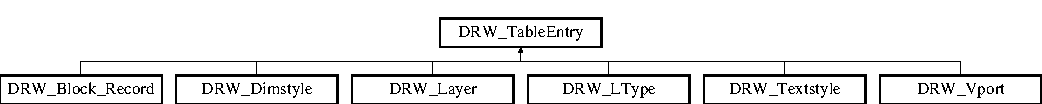
\includegraphics[height=1.393035cm]{de/d86/class_d_r_w___table_entry}
\end{center}
\end{figure}
\subsection*{Public Attributes}
\begin{DoxyCompactItemize}
\item 
enum D\+R\+W\+::\+T\+T\+Y\+P\+E \hyperlink{class_d_r_w___table_entry_a4ceb84db2231dcc1c3070e5825966a0d}{t\+Type}
\item 
int \hyperlink{class_d_r_w___table_entry_a9aefd859bd8a3d423f53623f8f089ac3}{handle}
\item 
int \hyperlink{class_d_r_w___table_entry_a91713970d0eec5baf8aa16b8c5556ce7}{handle\+Block}
\item 
U\+T\+F8\+S\+T\+R\+I\+N\+G \hyperlink{class_d_r_w___table_entry_a854ab48893457e607ac13425304415b4}{name}
\item 
int \hyperlink{class_d_r_w___table_entry_a45931e761e264e52857687067029e6a8}{flags}
\end{DoxyCompactItemize}
\subsection*{Protected Member Functions}
\begin{DoxyCompactItemize}
\item 
void \hyperlink{class_d_r_w___table_entry_ae342918d8e3005bd640762de9d52dbde}{parse\+Code} (int code, dxf\+Reader $\ast$reader)
\begin{DoxyCompactList}\small\item\em Base class for tables entries. \end{DoxyCompactList}\end{DoxyCompactItemize}


\subsection{Detailed Description}
Base class for tables entries. 

Base class for tables entries \begin{DoxyAuthor}{Author}
Rallaz 
\end{DoxyAuthor}


\subsection{Member Function Documentation}
\hypertarget{class_d_r_w___table_entry_ae342918d8e3005bd640762de9d52dbde}{}\index{D\+R\+W\+\_\+\+Table\+Entry@{D\+R\+W\+\_\+\+Table\+Entry}!parse\+Code@{parse\+Code}}
\index{parse\+Code@{parse\+Code}!D\+R\+W\+\_\+\+Table\+Entry@{D\+R\+W\+\_\+\+Table\+Entry}}
\subsubsection[{parse\+Code}]{\setlength{\rightskip}{0pt plus 5cm}void D\+R\+W\+\_\+\+Table\+Entry\+::parse\+Code (
\begin{DoxyParamCaption}
\item[{int}]{code, }
\item[{dxf\+Reader $\ast$}]{reader}
\end{DoxyParamCaption}
)\hspace{0.3cm}{\ttfamily [protected]}}\label{class_d_r_w___table_entry_ae342918d8e3005bd640762de9d52dbde}


Base class for tables entries. 

Base class for tables entries \begin{DoxyAuthor}{Author}
Rallaz 
\end{DoxyAuthor}


\subsection{Member Data Documentation}
\hypertarget{class_d_r_w___table_entry_a45931e761e264e52857687067029e6a8}{}\index{D\+R\+W\+\_\+\+Table\+Entry@{D\+R\+W\+\_\+\+Table\+Entry}!flags@{flags}}
\index{flags@{flags}!D\+R\+W\+\_\+\+Table\+Entry@{D\+R\+W\+\_\+\+Table\+Entry}}
\subsubsection[{flags}]{\setlength{\rightskip}{0pt plus 5cm}int D\+R\+W\+\_\+\+Table\+Entry\+::flags}\label{class_d_r_w___table_entry_a45931e761e264e52857687067029e6a8}
Flags relevant to entry, code 70 \hypertarget{class_d_r_w___table_entry_a9aefd859bd8a3d423f53623f8f089ac3}{}\index{D\+R\+W\+\_\+\+Table\+Entry@{D\+R\+W\+\_\+\+Table\+Entry}!handle@{handle}}
\index{handle@{handle}!D\+R\+W\+\_\+\+Table\+Entry@{D\+R\+W\+\_\+\+Table\+Entry}}
\subsubsection[{handle}]{\setlength{\rightskip}{0pt plus 5cm}int D\+R\+W\+\_\+\+Table\+Entry\+::handle}\label{class_d_r_w___table_entry_a9aefd859bd8a3d423f53623f8f089ac3}
entity identifier, code 5 \hypertarget{class_d_r_w___table_entry_a91713970d0eec5baf8aa16b8c5556ce7}{}\index{D\+R\+W\+\_\+\+Table\+Entry@{D\+R\+W\+\_\+\+Table\+Entry}!handle\+Block@{handle\+Block}}
\index{handle\+Block@{handle\+Block}!D\+R\+W\+\_\+\+Table\+Entry@{D\+R\+W\+\_\+\+Table\+Entry}}
\subsubsection[{handle\+Block}]{\setlength{\rightskip}{0pt plus 5cm}int D\+R\+W\+\_\+\+Table\+Entry\+::handle\+Block}\label{class_d_r_w___table_entry_a91713970d0eec5baf8aa16b8c5556ce7}
Soft-\/pointer I\+D/handle to owner B\+L\+O\+C\+K\+\_\+\+R\+E\+C\+O\+R\+D object, code 330 \hypertarget{class_d_r_w___table_entry_a854ab48893457e607ac13425304415b4}{}\index{D\+R\+W\+\_\+\+Table\+Entry@{D\+R\+W\+\_\+\+Table\+Entry}!name@{name}}
\index{name@{name}!D\+R\+W\+\_\+\+Table\+Entry@{D\+R\+W\+\_\+\+Table\+Entry}}
\subsubsection[{name}]{\setlength{\rightskip}{0pt plus 5cm}U\+T\+F8\+S\+T\+R\+I\+N\+G D\+R\+W\+\_\+\+Table\+Entry\+::name}\label{class_d_r_w___table_entry_a854ab48893457e607ac13425304415b4}
entry name, code 2 \hypertarget{class_d_r_w___table_entry_a4ceb84db2231dcc1c3070e5825966a0d}{}\index{D\+R\+W\+\_\+\+Table\+Entry@{D\+R\+W\+\_\+\+Table\+Entry}!t\+Type@{t\+Type}}
\index{t\+Type@{t\+Type}!D\+R\+W\+\_\+\+Table\+Entry@{D\+R\+W\+\_\+\+Table\+Entry}}
\subsubsection[{t\+Type}]{\setlength{\rightskip}{0pt plus 5cm}enum D\+R\+W\+::\+T\+T\+Y\+P\+E D\+R\+W\+\_\+\+Table\+Entry\+::t\+Type}\label{class_d_r_w___table_entry_a4ceb84db2231dcc1c3070e5825966a0d}
enum\+: entity type, code 0 

The documentation for this class was generated from the following files\+:\begin{DoxyCompactItemize}
\item 
src/drw\+\_\+objects.\+h\item 
src/drw\+\_\+objects.\+cpp\end{DoxyCompactItemize}

\hypertarget{class_d_r_w___text}{}\section{D\+R\+W\+\_\+\+Text Class Reference}
\label{class_d_r_w___text}\index{D\+R\+W\+\_\+\+Text@{D\+R\+W\+\_\+\+Text}}


Class to handle insert entries.  




{\ttfamily \#include $<$drw\+\_\+entities.\+h$>$}

Inheritance diagram for D\+R\+W\+\_\+\+Text\+:\begin{figure}[H]
\begin{center}
\leavevmode
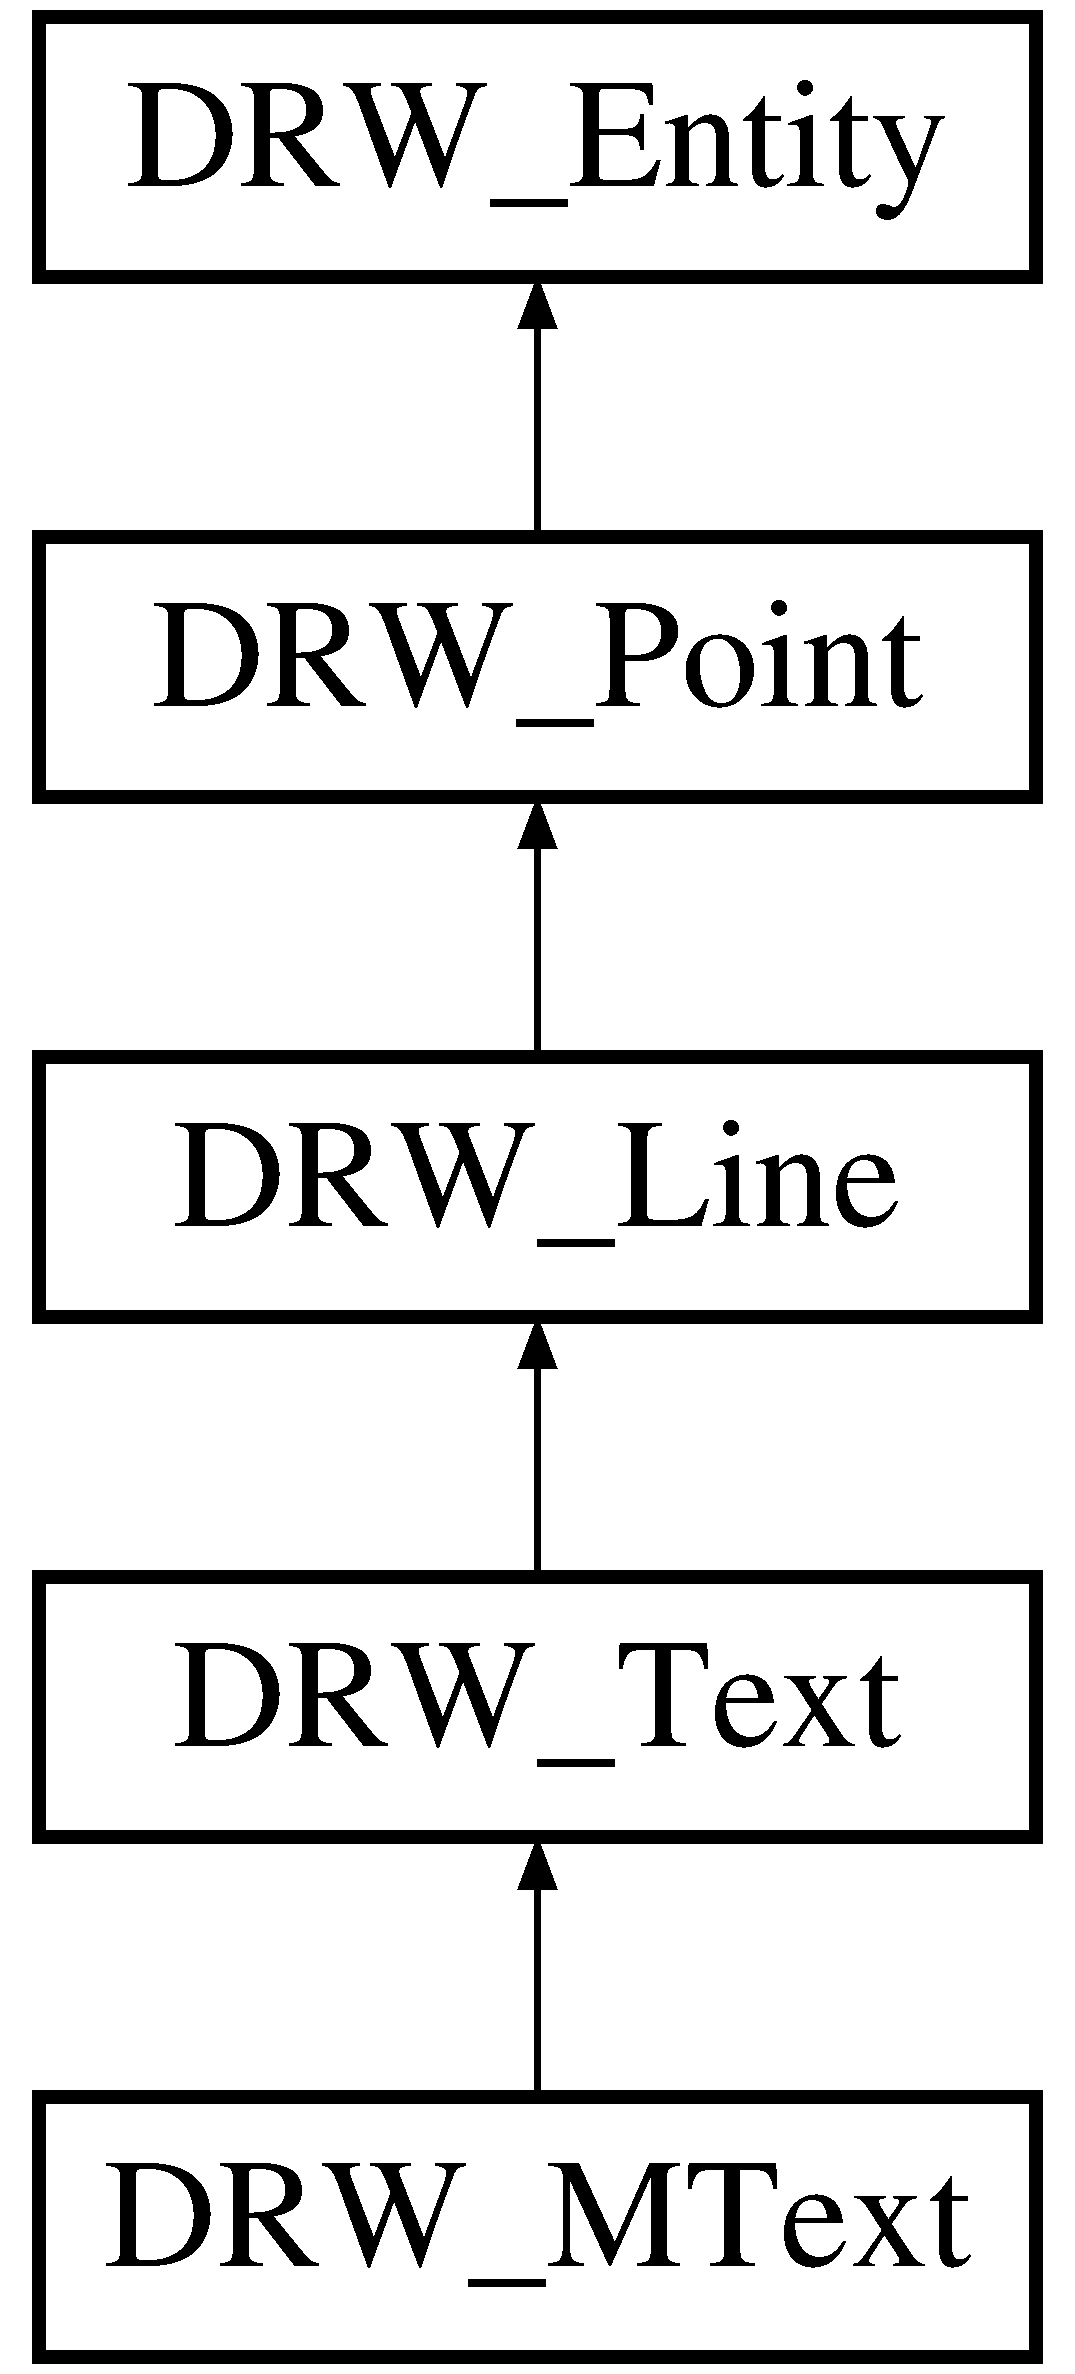
\includegraphics[height=5.000000cm]{d9/d65/class_d_r_w___text}
\end{center}
\end{figure}
\subsection*{Public Types}
\begin{DoxyCompactItemize}
\item 
enum \hyperlink{class_d_r_w___text_a369c571137713ac08c5a5a9b66ff6c27}{V\+Align} \{ \hyperlink{class_d_r_w___text_a369c571137713ac08c5a5a9b66ff6c27a26e0d96529d0c6edf8fe94c09ffd1661}{V\+Base\+Line} = 0, 
\hyperlink{class_d_r_w___text_a369c571137713ac08c5a5a9b66ff6c27a64c2355b0923f0634c45002f571c9fba}{V\+Bottom}, 
\hyperlink{class_d_r_w___text_a369c571137713ac08c5a5a9b66ff6c27adf2dfb4d3e854d4c660246808495152e}{V\+Middle}, 
\hyperlink{class_d_r_w___text_a369c571137713ac08c5a5a9b66ff6c27ad6c53af0a564a39018d403af25aa97e3}{V\+Top}
 \}
\begin{DoxyCompactList}\small\item\em Vertical alignments. \end{DoxyCompactList}\item 
enum \hyperlink{class_d_r_w___text_a66511da21199b0ab967fa951bc339f2d}{H\+Align} \{ \\*
\hyperlink{class_d_r_w___text_a66511da21199b0ab967fa951bc339f2da2fca970851f2bddb3f018307e47f653c}{H\+Left} = 0, 
\hyperlink{class_d_r_w___text_a66511da21199b0ab967fa951bc339f2dacae7fa84a0beaf06577027631f445225}{H\+Center}, 
\hyperlink{class_d_r_w___text_a66511da21199b0ab967fa951bc339f2dafc3e7b70ef3f4cb5bf2228f0fe2dfc8f}{H\+Right}, 
\hyperlink{class_d_r_w___text_a66511da21199b0ab967fa951bc339f2da3f5e5f69673e0b948de41c8e16ffd131}{H\+Aligned}, 
\\*
\hyperlink{class_d_r_w___text_a66511da21199b0ab967fa951bc339f2da9705528a85e9416e32dbb959ad22a584}{H\+Middle}, 
\hyperlink{class_d_r_w___text_a66511da21199b0ab967fa951bc339f2da3b8fe44dc62bffe5c97d7b96ef1b3c23}{H\+Fit}
 \}
\begin{DoxyCompactList}\small\item\em Horizontal alignments. \end{DoxyCompactList}\end{DoxyCompactItemize}
\subsection*{Public Attributes}
\begin{DoxyCompactItemize}
\item 
double \hyperlink{class_d_r_w___text_ad38ec2dfef3ab3c4367423a0d4e49c05}{height}
\item 
U\+T\+F8\+S\+T\+R\+I\+N\+G \hyperlink{class_d_r_w___text_a87a40d4523371ee0cc250be0fc8834cd}{text}
\item 
double \hyperlink{class_d_r_w___text_aad647ab8b0086a18978dd0b291569e5b}{angle}
\item 
double \hyperlink{class_d_r_w___text_a17468f7c0e1bd0b1c6da87cc9300b7e1}{widthscale}
\item 
double \hyperlink{class_d_r_w___text_ab273757633e67aa82b17b6b1141c8b98}{oblique}
\item 
U\+T\+F8\+S\+T\+R\+I\+N\+G \hyperlink{class_d_r_w___text_a11fa7c1b5a6fccafe2991bad2413cfa8}{style}
\item 
int \hyperlink{class_d_r_w___text_ada45df3aae10844afc1861261e40869e}{textgen}
\item 
enum \hyperlink{class_d_r_w___text_a66511da21199b0ab967fa951bc339f2d}{H\+Align} \hyperlink{class_d_r_w___text_ace4ad466c2d13111f69b4413c279987e}{align\+H}
\item 
enum \hyperlink{class_d_r_w___text_a369c571137713ac08c5a5a9b66ff6c27}{V\+Align} \hyperlink{class_d_r_w___text_a1b3c6431eb7c016e3521a46dc24bd57e}{align\+V}
\item 
\hyperlink{classdwg_handle}{dwg\+Handle} \hyperlink{class_d_r_w___text_a2bbd98f55b08ef9d9d7011a32c6d94dd}{style\+H}
\end{DoxyCompactItemize}
\subsection*{Additional Inherited Members}


\subsection{Detailed Description}
Class to handle insert entries. 

Class to handle insert entries \begin{DoxyAuthor}{Author}
Rallaz 
\end{DoxyAuthor}


\subsection{Member Enumeration Documentation}
\hypertarget{class_d_r_w___text_a66511da21199b0ab967fa951bc339f2d}{}\index{D\+R\+W\+\_\+\+Text@{D\+R\+W\+\_\+\+Text}!H\+Align@{H\+Align}}
\index{H\+Align@{H\+Align}!D\+R\+W\+\_\+\+Text@{D\+R\+W\+\_\+\+Text}}
\subsubsection[{H\+Align}]{\setlength{\rightskip}{0pt plus 5cm}enum {\bf D\+R\+W\+\_\+\+Text\+::\+H\+Align}}\label{class_d_r_w___text_a66511da21199b0ab967fa951bc339f2d}


Horizontal alignments. 

\begin{Desc}
\item[Enumerator]\par
\begin{description}
\index{H\+Left@{H\+Left}!D\+R\+W\+\_\+\+Text@{D\+R\+W\+\_\+\+Text}}\index{D\+R\+W\+\_\+\+Text@{D\+R\+W\+\_\+\+Text}!H\+Left@{H\+Left}}\item[{\em 
\hypertarget{class_d_r_w___text_a66511da21199b0ab967fa951bc339f2da2fca970851f2bddb3f018307e47f653c}{}H\+Left\label{class_d_r_w___text_a66511da21199b0ab967fa951bc339f2da2fca970851f2bddb3f018307e47f653c}
}]Left = 0 \index{H\+Center@{H\+Center}!D\+R\+W\+\_\+\+Text@{D\+R\+W\+\_\+\+Text}}\index{D\+R\+W\+\_\+\+Text@{D\+R\+W\+\_\+\+Text}!H\+Center@{H\+Center}}\item[{\em 
\hypertarget{class_d_r_w___text_a66511da21199b0ab967fa951bc339f2dacae7fa84a0beaf06577027631f445225}{}H\+Center\label{class_d_r_w___text_a66511da21199b0ab967fa951bc339f2dacae7fa84a0beaf06577027631f445225}
}]Centered = 1 \index{H\+Right@{H\+Right}!D\+R\+W\+\_\+\+Text@{D\+R\+W\+\_\+\+Text}}\index{D\+R\+W\+\_\+\+Text@{D\+R\+W\+\_\+\+Text}!H\+Right@{H\+Right}}\item[{\em 
\hypertarget{class_d_r_w___text_a66511da21199b0ab967fa951bc339f2dafc3e7b70ef3f4cb5bf2228f0fe2dfc8f}{}H\+Right\label{class_d_r_w___text_a66511da21199b0ab967fa951bc339f2dafc3e7b70ef3f4cb5bf2228f0fe2dfc8f}
}]Right = 2 \index{H\+Aligned@{H\+Aligned}!D\+R\+W\+\_\+\+Text@{D\+R\+W\+\_\+\+Text}}\index{D\+R\+W\+\_\+\+Text@{D\+R\+W\+\_\+\+Text}!H\+Aligned@{H\+Aligned}}\item[{\em 
\hypertarget{class_d_r_w___text_a66511da21199b0ab967fa951bc339f2da3f5e5f69673e0b948de41c8e16ffd131}{}H\+Aligned\label{class_d_r_w___text_a66511da21199b0ab967fa951bc339f2da3f5e5f69673e0b948de41c8e16ffd131}
}]Aligned = 3 (if V\+Align==0) \index{H\+Middle@{H\+Middle}!D\+R\+W\+\_\+\+Text@{D\+R\+W\+\_\+\+Text}}\index{D\+R\+W\+\_\+\+Text@{D\+R\+W\+\_\+\+Text}!H\+Middle@{H\+Middle}}\item[{\em 
\hypertarget{class_d_r_w___text_a66511da21199b0ab967fa951bc339f2da9705528a85e9416e32dbb959ad22a584}{}H\+Middle\label{class_d_r_w___text_a66511da21199b0ab967fa951bc339f2da9705528a85e9416e32dbb959ad22a584}
}]middle = 4 (if V\+Align==0) \index{H\+Fit@{H\+Fit}!D\+R\+W\+\_\+\+Text@{D\+R\+W\+\_\+\+Text}}\index{D\+R\+W\+\_\+\+Text@{D\+R\+W\+\_\+\+Text}!H\+Fit@{H\+Fit}}\item[{\em 
\hypertarget{class_d_r_w___text_a66511da21199b0ab967fa951bc339f2da3b8fe44dc62bffe5c97d7b96ef1b3c23}{}H\+Fit\label{class_d_r_w___text_a66511da21199b0ab967fa951bc339f2da3b8fe44dc62bffe5c97d7b96ef1b3c23}
}]fit into point = 5 (if V\+Align==0) \end{description}
\end{Desc}
\hypertarget{class_d_r_w___text_a369c571137713ac08c5a5a9b66ff6c27}{}\index{D\+R\+W\+\_\+\+Text@{D\+R\+W\+\_\+\+Text}!V\+Align@{V\+Align}}
\index{V\+Align@{V\+Align}!D\+R\+W\+\_\+\+Text@{D\+R\+W\+\_\+\+Text}}
\subsubsection[{V\+Align}]{\setlength{\rightskip}{0pt plus 5cm}enum {\bf D\+R\+W\+\_\+\+Text\+::\+V\+Align}}\label{class_d_r_w___text_a369c571137713ac08c5a5a9b66ff6c27}


Vertical alignments. 

\begin{Desc}
\item[Enumerator]\par
\begin{description}
\index{V\+Base\+Line@{V\+Base\+Line}!D\+R\+W\+\_\+\+Text@{D\+R\+W\+\_\+\+Text}}\index{D\+R\+W\+\_\+\+Text@{D\+R\+W\+\_\+\+Text}!V\+Base\+Line@{V\+Base\+Line}}\item[{\em 
\hypertarget{class_d_r_w___text_a369c571137713ac08c5a5a9b66ff6c27a26e0d96529d0c6edf8fe94c09ffd1661}{}V\+Base\+Line\label{class_d_r_w___text_a369c571137713ac08c5a5a9b66ff6c27a26e0d96529d0c6edf8fe94c09ffd1661}
}]Top = 0 \index{V\+Bottom@{V\+Bottom}!D\+R\+W\+\_\+\+Text@{D\+R\+W\+\_\+\+Text}}\index{D\+R\+W\+\_\+\+Text@{D\+R\+W\+\_\+\+Text}!V\+Bottom@{V\+Bottom}}\item[{\em 
\hypertarget{class_d_r_w___text_a369c571137713ac08c5a5a9b66ff6c27a64c2355b0923f0634c45002f571c9fba}{}V\+Bottom\label{class_d_r_w___text_a369c571137713ac08c5a5a9b66ff6c27a64c2355b0923f0634c45002f571c9fba}
}]Bottom = 1 \index{V\+Middle@{V\+Middle}!D\+R\+W\+\_\+\+Text@{D\+R\+W\+\_\+\+Text}}\index{D\+R\+W\+\_\+\+Text@{D\+R\+W\+\_\+\+Text}!V\+Middle@{V\+Middle}}\item[{\em 
\hypertarget{class_d_r_w___text_a369c571137713ac08c5a5a9b66ff6c27adf2dfb4d3e854d4c660246808495152e}{}V\+Middle\label{class_d_r_w___text_a369c571137713ac08c5a5a9b66ff6c27adf2dfb4d3e854d4c660246808495152e}
}]Middle = 2 \index{V\+Top@{V\+Top}!D\+R\+W\+\_\+\+Text@{D\+R\+W\+\_\+\+Text}}\index{D\+R\+W\+\_\+\+Text@{D\+R\+W\+\_\+\+Text}!V\+Top@{V\+Top}}\item[{\em 
\hypertarget{class_d_r_w___text_a369c571137713ac08c5a5a9b66ff6c27ad6c53af0a564a39018d403af25aa97e3}{}V\+Top\label{class_d_r_w___text_a369c571137713ac08c5a5a9b66ff6c27ad6c53af0a564a39018d403af25aa97e3}
}]Top = 3 \end{description}
\end{Desc}


\subsection{Member Data Documentation}
\hypertarget{class_d_r_w___text_ace4ad466c2d13111f69b4413c279987e}{}\index{D\+R\+W\+\_\+\+Text@{D\+R\+W\+\_\+\+Text}!align\+H@{align\+H}}
\index{align\+H@{align\+H}!D\+R\+W\+\_\+\+Text@{D\+R\+W\+\_\+\+Text}}
\subsubsection[{align\+H}]{\setlength{\rightskip}{0pt plus 5cm}enum {\bf H\+Align} D\+R\+W\+\_\+\+Text\+::align\+H}\label{class_d_r_w___text_ace4ad466c2d13111f69b4413c279987e}
horizontal align, code 72 \hypertarget{class_d_r_w___text_a1b3c6431eb7c016e3521a46dc24bd57e}{}\index{D\+R\+W\+\_\+\+Text@{D\+R\+W\+\_\+\+Text}!align\+V@{align\+V}}
\index{align\+V@{align\+V}!D\+R\+W\+\_\+\+Text@{D\+R\+W\+\_\+\+Text}}
\subsubsection[{align\+V}]{\setlength{\rightskip}{0pt plus 5cm}enum {\bf V\+Align} D\+R\+W\+\_\+\+Text\+::align\+V}\label{class_d_r_w___text_a1b3c6431eb7c016e3521a46dc24bd57e}
vertical align, code 73 \hypertarget{class_d_r_w___text_aad647ab8b0086a18978dd0b291569e5b}{}\index{D\+R\+W\+\_\+\+Text@{D\+R\+W\+\_\+\+Text}!angle@{angle}}
\index{angle@{angle}!D\+R\+W\+\_\+\+Text@{D\+R\+W\+\_\+\+Text}}
\subsubsection[{angle}]{\setlength{\rightskip}{0pt plus 5cm}double D\+R\+W\+\_\+\+Text\+::angle}\label{class_d_r_w___text_aad647ab8b0086a18978dd0b291569e5b}
rotation angle in degrees (360), code 50 \hypertarget{class_d_r_w___text_ad38ec2dfef3ab3c4367423a0d4e49c05}{}\index{D\+R\+W\+\_\+\+Text@{D\+R\+W\+\_\+\+Text}!height@{height}}
\index{height@{height}!D\+R\+W\+\_\+\+Text@{D\+R\+W\+\_\+\+Text}}
\subsubsection[{height}]{\setlength{\rightskip}{0pt plus 5cm}double D\+R\+W\+\_\+\+Text\+::height}\label{class_d_r_w___text_ad38ec2dfef3ab3c4367423a0d4e49c05}
height text, code 40 \hypertarget{class_d_r_w___text_ab273757633e67aa82b17b6b1141c8b98}{}\index{D\+R\+W\+\_\+\+Text@{D\+R\+W\+\_\+\+Text}!oblique@{oblique}}
\index{oblique@{oblique}!D\+R\+W\+\_\+\+Text@{D\+R\+W\+\_\+\+Text}}
\subsubsection[{oblique}]{\setlength{\rightskip}{0pt plus 5cm}double D\+R\+W\+\_\+\+Text\+::oblique}\label{class_d_r_w___text_ab273757633e67aa82b17b6b1141c8b98}
oblique angle, code 51 \hypertarget{class_d_r_w___text_a11fa7c1b5a6fccafe2991bad2413cfa8}{}\index{D\+R\+W\+\_\+\+Text@{D\+R\+W\+\_\+\+Text}!style@{style}}
\index{style@{style}!D\+R\+W\+\_\+\+Text@{D\+R\+W\+\_\+\+Text}}
\subsubsection[{style}]{\setlength{\rightskip}{0pt plus 5cm}U\+T\+F8\+S\+T\+R\+I\+N\+G D\+R\+W\+\_\+\+Text\+::style}\label{class_d_r_w___text_a11fa7c1b5a6fccafe2991bad2413cfa8}
style name, code 7 \hypertarget{class_d_r_w___text_a2bbd98f55b08ef9d9d7011a32c6d94dd}{}\index{D\+R\+W\+\_\+\+Text@{D\+R\+W\+\_\+\+Text}!style\+H@{style\+H}}
\index{style\+H@{style\+H}!D\+R\+W\+\_\+\+Text@{D\+R\+W\+\_\+\+Text}}
\subsubsection[{style\+H}]{\setlength{\rightskip}{0pt plus 5cm}{\bf dwg\+Handle} D\+R\+W\+\_\+\+Text\+::style\+H}\label{class_d_r_w___text_a2bbd98f55b08ef9d9d7011a32c6d94dd}
handle for text style \hypertarget{class_d_r_w___text_a87a40d4523371ee0cc250be0fc8834cd}{}\index{D\+R\+W\+\_\+\+Text@{D\+R\+W\+\_\+\+Text}!text@{text}}
\index{text@{text}!D\+R\+W\+\_\+\+Text@{D\+R\+W\+\_\+\+Text}}
\subsubsection[{text}]{\setlength{\rightskip}{0pt plus 5cm}U\+T\+F8\+S\+T\+R\+I\+N\+G D\+R\+W\+\_\+\+Text\+::text}\label{class_d_r_w___text_a87a40d4523371ee0cc250be0fc8834cd}
text string, code 1 \hypertarget{class_d_r_w___text_ada45df3aae10844afc1861261e40869e}{}\index{D\+R\+W\+\_\+\+Text@{D\+R\+W\+\_\+\+Text}!textgen@{textgen}}
\index{textgen@{textgen}!D\+R\+W\+\_\+\+Text@{D\+R\+W\+\_\+\+Text}}
\subsubsection[{textgen}]{\setlength{\rightskip}{0pt plus 5cm}int D\+R\+W\+\_\+\+Text\+::textgen}\label{class_d_r_w___text_ada45df3aae10844afc1861261e40869e}
text generation, code 71 \hypertarget{class_d_r_w___text_a17468f7c0e1bd0b1c6da87cc9300b7e1}{}\index{D\+R\+W\+\_\+\+Text@{D\+R\+W\+\_\+\+Text}!widthscale@{widthscale}}
\index{widthscale@{widthscale}!D\+R\+W\+\_\+\+Text@{D\+R\+W\+\_\+\+Text}}
\subsubsection[{widthscale}]{\setlength{\rightskip}{0pt plus 5cm}double D\+R\+W\+\_\+\+Text\+::widthscale}\label{class_d_r_w___text_a17468f7c0e1bd0b1c6da87cc9300b7e1}
width factor, code 41 

The documentation for this class was generated from the following files\+:\begin{DoxyCompactItemize}
\item 
src/drw\+\_\+entities.\+h\item 
src/drw\+\_\+entities.\+cpp\end{DoxyCompactItemize}

\hypertarget{class_d_r_w___textstyle}{}\section{D\+R\+W\+\_\+\+Textstyle Class Reference}
\label{class_d_r_w___textstyle}\index{D\+R\+W\+\_\+\+Textstyle@{D\+R\+W\+\_\+\+Textstyle}}


Class to handle text style entries.  




{\ttfamily \#include $<$drw\+\_\+objects.\+h$>$}

Inheritance diagram for D\+R\+W\+\_\+\+Textstyle\+:\begin{figure}[H]
\begin{center}
\leavevmode
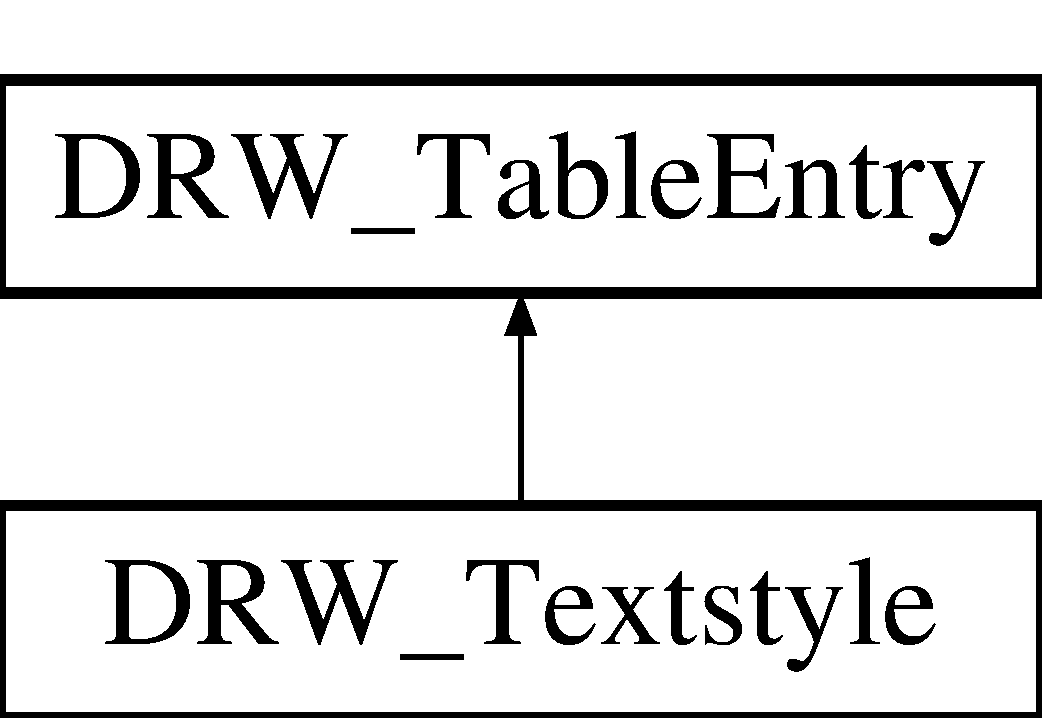
\includegraphics[height=2.000000cm]{df/d54/class_d_r_w___textstyle}
\end{center}
\end{figure}
\subsection*{Public Member Functions}
\begin{DoxyCompactItemize}
\item 
void \hyperlink{class_d_r_w___textstyle_a05f7de5ef7082ac33bbc61908dfc7c24}{parse\+Code} (int code, dxf\+Reader $\ast$reader)
\begin{DoxyCompactList}\small\item\em Class to handle text style entries. \end{DoxyCompactList}\end{DoxyCompactItemize}
\subsection*{Public Attributes}
\begin{DoxyCompactItemize}
\item 
double \hyperlink{class_d_r_w___textstyle_a23809c13d923ae1ae43dc83c2f200e47}{height}
\item 
double \hyperlink{class_d_r_w___textstyle_a36bce344a959c198199e88482ede075a}{width}
\item 
double \hyperlink{class_d_r_w___textstyle_a5d133a89292ecc76b6a66af88039c6cc}{oblique}
\item 
int \hyperlink{class_d_r_w___textstyle_adec337333f98e34908076b2b1a0a10a0}{gen\+Flag}
\item 
double \hyperlink{class_d_r_w___textstyle_ad7c6c347da9dfa658fabeeb46e430da4}{last\+Height}
\item 
U\+T\+F8\+S\+T\+R\+I\+N\+G \hyperlink{class_d_r_w___textstyle_ac04f9a321fbb47a3adc3aaf65b30f02b}{font}
\item 
U\+T\+F8\+S\+T\+R\+I\+N\+G \hyperlink{class_d_r_w___textstyle_a5e5bee24192efcdc25e2922c2639a73e}{big\+Font}
\item 
int \hyperlink{class_d_r_w___textstyle_a40ef37c402a0f1b75f481be925c85357}{font\+Family}
\end{DoxyCompactItemize}
\subsection*{Additional Inherited Members}


\subsection{Detailed Description}
Class to handle text style entries. 

Class to handle text style symbol table entries \begin{DoxyAuthor}{Author}
Rallaz 
\end{DoxyAuthor}


\subsection{Member Function Documentation}
\hypertarget{class_d_r_w___textstyle_a05f7de5ef7082ac33bbc61908dfc7c24}{}\index{D\+R\+W\+\_\+\+Textstyle@{D\+R\+W\+\_\+\+Textstyle}!parse\+Code@{parse\+Code}}
\index{parse\+Code@{parse\+Code}!D\+R\+W\+\_\+\+Textstyle@{D\+R\+W\+\_\+\+Textstyle}}
\subsubsection[{parse\+Code}]{\setlength{\rightskip}{0pt plus 5cm}void D\+R\+W\+\_\+\+Textstyle\+::parse\+Code (
\begin{DoxyParamCaption}
\item[{int}]{code, }
\item[{dxf\+Reader $\ast$}]{reader}
\end{DoxyParamCaption}
)}\label{class_d_r_w___textstyle_a05f7de5ef7082ac33bbc61908dfc7c24}


Class to handle text style entries. 

Class to handle text style symbol table entries \begin{DoxyAuthor}{Author}
Rallaz 
\end{DoxyAuthor}


\subsection{Member Data Documentation}
\hypertarget{class_d_r_w___textstyle_a5e5bee24192efcdc25e2922c2639a73e}{}\index{D\+R\+W\+\_\+\+Textstyle@{D\+R\+W\+\_\+\+Textstyle}!big\+Font@{big\+Font}}
\index{big\+Font@{big\+Font}!D\+R\+W\+\_\+\+Textstyle@{D\+R\+W\+\_\+\+Textstyle}}
\subsubsection[{big\+Font}]{\setlength{\rightskip}{0pt plus 5cm}U\+T\+F8\+S\+T\+R\+I\+N\+G D\+R\+W\+\_\+\+Textstyle\+::big\+Font}\label{class_d_r_w___textstyle_a5e5bee24192efcdc25e2922c2639a73e}
bigfont file name or blank if none, code 4 \hypertarget{class_d_r_w___textstyle_ac04f9a321fbb47a3adc3aaf65b30f02b}{}\index{D\+R\+W\+\_\+\+Textstyle@{D\+R\+W\+\_\+\+Textstyle}!font@{font}}
\index{font@{font}!D\+R\+W\+\_\+\+Textstyle@{D\+R\+W\+\_\+\+Textstyle}}
\subsubsection[{font}]{\setlength{\rightskip}{0pt plus 5cm}U\+T\+F8\+S\+T\+R\+I\+N\+G D\+R\+W\+\_\+\+Textstyle\+::font}\label{class_d_r_w___textstyle_ac04f9a321fbb47a3adc3aaf65b30f02b}
primary font file name, code 3 \hypertarget{class_d_r_w___textstyle_a40ef37c402a0f1b75f481be925c85357}{}\index{D\+R\+W\+\_\+\+Textstyle@{D\+R\+W\+\_\+\+Textstyle}!font\+Family@{font\+Family}}
\index{font\+Family@{font\+Family}!D\+R\+W\+\_\+\+Textstyle@{D\+R\+W\+\_\+\+Textstyle}}
\subsubsection[{font\+Family}]{\setlength{\rightskip}{0pt plus 5cm}int D\+R\+W\+\_\+\+Textstyle\+::font\+Family}\label{class_d_r_w___textstyle_a40ef37c402a0f1b75f481be925c85357}
ttf font family, italic and bold flags, code 1071 \hypertarget{class_d_r_w___textstyle_adec337333f98e34908076b2b1a0a10a0}{}\index{D\+R\+W\+\_\+\+Textstyle@{D\+R\+W\+\_\+\+Textstyle}!gen\+Flag@{gen\+Flag}}
\index{gen\+Flag@{gen\+Flag}!D\+R\+W\+\_\+\+Textstyle@{D\+R\+W\+\_\+\+Textstyle}}
\subsubsection[{gen\+Flag}]{\setlength{\rightskip}{0pt plus 5cm}int D\+R\+W\+\_\+\+Textstyle\+::gen\+Flag}\label{class_d_r_w___textstyle_adec337333f98e34908076b2b1a0a10a0}
Text generation flags, code 71 \hypertarget{class_d_r_w___textstyle_a23809c13d923ae1ae43dc83c2f200e47}{}\index{D\+R\+W\+\_\+\+Textstyle@{D\+R\+W\+\_\+\+Textstyle}!height@{height}}
\index{height@{height}!D\+R\+W\+\_\+\+Textstyle@{D\+R\+W\+\_\+\+Textstyle}}
\subsubsection[{height}]{\setlength{\rightskip}{0pt plus 5cm}double D\+R\+W\+\_\+\+Textstyle\+::height}\label{class_d_r_w___textstyle_a23809c13d923ae1ae43dc83c2f200e47}
Fixed text height (0 not set), code 40 \hypertarget{class_d_r_w___textstyle_ad7c6c347da9dfa658fabeeb46e430da4}{}\index{D\+R\+W\+\_\+\+Textstyle@{D\+R\+W\+\_\+\+Textstyle}!last\+Height@{last\+Height}}
\index{last\+Height@{last\+Height}!D\+R\+W\+\_\+\+Textstyle@{D\+R\+W\+\_\+\+Textstyle}}
\subsubsection[{last\+Height}]{\setlength{\rightskip}{0pt plus 5cm}double D\+R\+W\+\_\+\+Textstyle\+::last\+Height}\label{class_d_r_w___textstyle_ad7c6c347da9dfa658fabeeb46e430da4}
Last height used, code 42 \hypertarget{class_d_r_w___textstyle_a5d133a89292ecc76b6a66af88039c6cc}{}\index{D\+R\+W\+\_\+\+Textstyle@{D\+R\+W\+\_\+\+Textstyle}!oblique@{oblique}}
\index{oblique@{oblique}!D\+R\+W\+\_\+\+Textstyle@{D\+R\+W\+\_\+\+Textstyle}}
\subsubsection[{oblique}]{\setlength{\rightskip}{0pt plus 5cm}double D\+R\+W\+\_\+\+Textstyle\+::oblique}\label{class_d_r_w___textstyle_a5d133a89292ecc76b6a66af88039c6cc}
Oblique angle, code 50 \hypertarget{class_d_r_w___textstyle_a36bce344a959c198199e88482ede075a}{}\index{D\+R\+W\+\_\+\+Textstyle@{D\+R\+W\+\_\+\+Textstyle}!width@{width}}
\index{width@{width}!D\+R\+W\+\_\+\+Textstyle@{D\+R\+W\+\_\+\+Textstyle}}
\subsubsection[{width}]{\setlength{\rightskip}{0pt plus 5cm}double D\+R\+W\+\_\+\+Textstyle\+::width}\label{class_d_r_w___textstyle_a36bce344a959c198199e88482ede075a}
Width factor, code 41 

The documentation for this class was generated from the following files\+:\begin{DoxyCompactItemize}
\item 
src/drw\+\_\+objects.\+h\item 
src/drw\+\_\+objects.\+cpp\end{DoxyCompactItemize}

\hypertarget{class_d_r_w___trace}{}\section{D\+R\+W\+\_\+\+Trace Class Reference}
\label{class_d_r_w___trace}\index{D\+R\+W\+\_\+\+Trace@{D\+R\+W\+\_\+\+Trace}}


Class to handle trace entity.  




{\ttfamily \#include $<$drw\+\_\+entities.\+h$>$}

Inheritance diagram for D\+R\+W\+\_\+\+Trace\+:\begin{figure}[H]
\begin{center}
\leavevmode
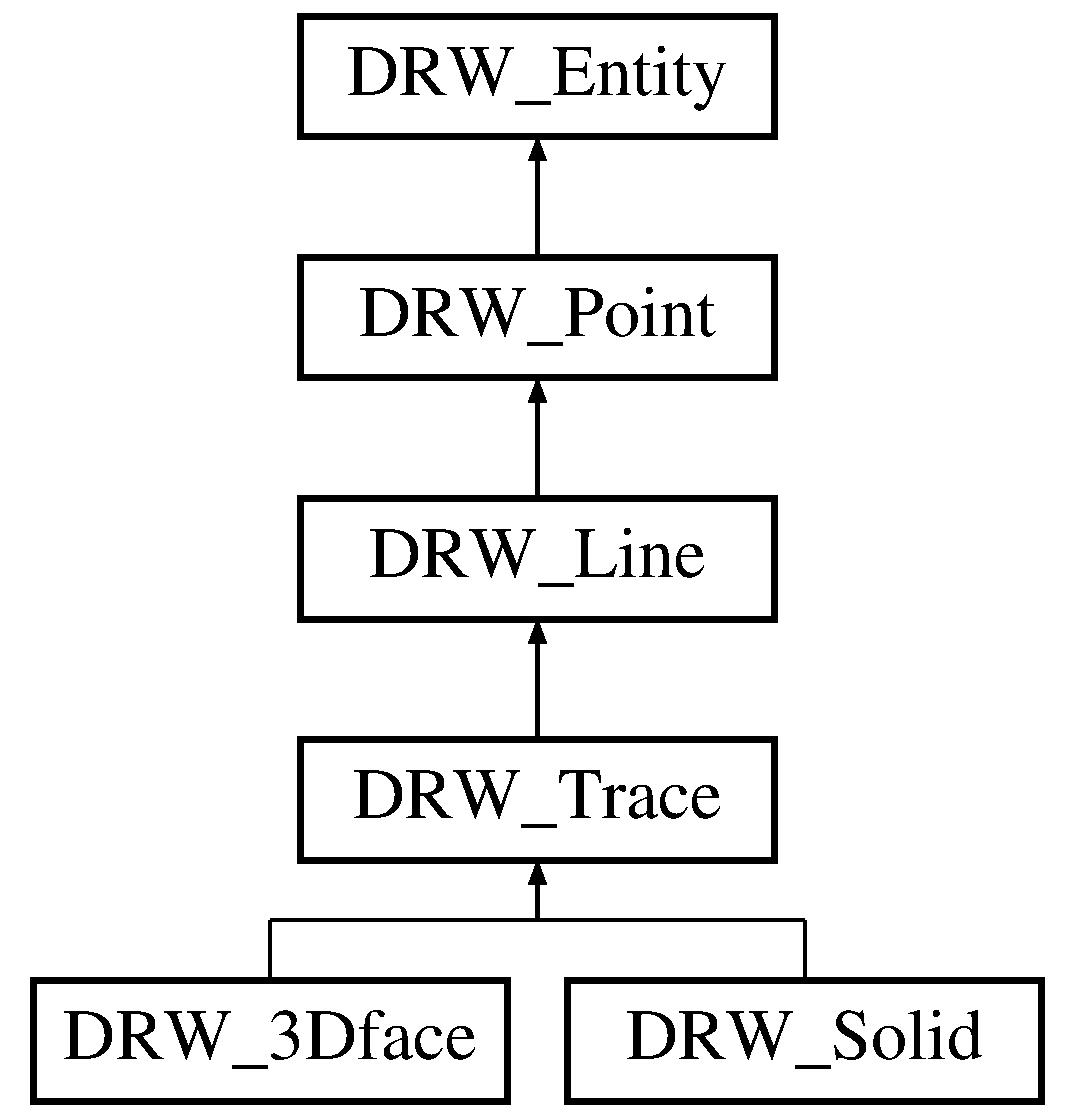
\includegraphics[height=5.000000cm]{d2/d52/class_d_r_w___trace}
\end{center}
\end{figure}
\subsection*{Public Attributes}
\begin{DoxyCompactItemize}
\item 
\hyperlink{class_d_r_w___coord}{D\+R\+W\+\_\+\+Coord} \hyperlink{class_d_r_w___trace_adadabbf354ee19cfe3869c790e6de3ec}{third\+Point}
\item 
\hyperlink{class_d_r_w___coord}{D\+R\+W\+\_\+\+Coord} \hyperlink{class_d_r_w___trace_a96d7a3b877a7f26f6a8b8cdbc9ced660}{four\+Point}
\end{DoxyCompactItemize}
\subsection*{Friends}
\begin{DoxyCompactItemize}
\item 
\hypertarget{class_d_r_w___trace_a7f080e77e5112f8364c61b97387f8ee2}{}class {\bfseries dxf\+R\+W}\label{class_d_r_w___trace_a7f080e77e5112f8364c61b97387f8ee2}

\end{DoxyCompactItemize}
\subsection*{Additional Inherited Members}


\subsection{Detailed Description}
Class to handle trace entity. 

Class to handle trace entity \begin{DoxyAuthor}{Author}
Rallaz 
\end{DoxyAuthor}


\subsection{Member Data Documentation}
\hypertarget{class_d_r_w___trace_a96d7a3b877a7f26f6a8b8cdbc9ced660}{}\index{D\+R\+W\+\_\+\+Trace@{D\+R\+W\+\_\+\+Trace}!four\+Point@{four\+Point}}
\index{four\+Point@{four\+Point}!D\+R\+W\+\_\+\+Trace@{D\+R\+W\+\_\+\+Trace}}
\subsubsection[{four\+Point}]{\setlength{\rightskip}{0pt plus 5cm}{\bf D\+R\+W\+\_\+\+Coord} D\+R\+W\+\_\+\+Trace\+::four\+Point}\label{class_d_r_w___trace_a96d7a3b877a7f26f6a8b8cdbc9ced660}
four point, code 13, 23 \& 33 \hypertarget{class_d_r_w___trace_adadabbf354ee19cfe3869c790e6de3ec}{}\index{D\+R\+W\+\_\+\+Trace@{D\+R\+W\+\_\+\+Trace}!third\+Point@{third\+Point}}
\index{third\+Point@{third\+Point}!D\+R\+W\+\_\+\+Trace@{D\+R\+W\+\_\+\+Trace}}
\subsubsection[{third\+Point}]{\setlength{\rightskip}{0pt plus 5cm}{\bf D\+R\+W\+\_\+\+Coord} D\+R\+W\+\_\+\+Trace\+::third\+Point}\label{class_d_r_w___trace_adadabbf354ee19cfe3869c790e6de3ec}
third point, code 12, 22 \& 32 

The documentation for this class was generated from the following files\+:\begin{DoxyCompactItemize}
\item 
src/drw\+\_\+entities.\+h\item 
src/drw\+\_\+entities.\+cpp\end{DoxyCompactItemize}

\hypertarget{union_d_r_w___variant_1_1_d_r_w___var_content}{}\section{D\+R\+W\+\_\+\+Variant\+:\+:D\+R\+W\+\_\+\+Var\+Content Union Reference}
\label{union_d_r_w___variant_1_1_d_r_w___var_content}\index{D\+R\+W\+\_\+\+Variant\+::\+D\+R\+W\+\_\+\+Var\+Content@{D\+R\+W\+\_\+\+Variant\+::\+D\+R\+W\+\_\+\+Var\+Content}}


The documentation for this union was generated from the following file\+:\begin{DoxyCompactItemize}
\item 
src/drw\+\_\+base.\+h\end{DoxyCompactItemize}

\hypertarget{class_d_r_w___variant}{}\section{D\+R\+W\+\_\+\+Variant Class Reference}
\label{class_d_r_w___variant}\index{D\+R\+W\+\_\+\+Variant@{D\+R\+W\+\_\+\+Variant}}


Class to handle header vars.  




{\ttfamily \#include $<$drw\+\_\+base.\+h$>$}

\subsection*{Classes}
\begin{DoxyCompactItemize}
\item 
union \hyperlink{union_d_r_w___variant_1_1_d_r_w___var_content}{D\+R\+W\+\_\+\+Var\+Content}
\end{DoxyCompactItemize}


\subsection{Detailed Description}
Class to handle header vars. 

Class to handle header vars \begin{DoxyAuthor}{Author}
Rallaz 
\end{DoxyAuthor}


The documentation for this class was generated from the following file\+:\begin{DoxyCompactItemize}
\item 
src/drw\+\_\+base.\+h\end{DoxyCompactItemize}

\hypertarget{class_d_r_w___vertex}{}\section{D\+R\+W\+\_\+\+Vertex Class Reference}
\label{class_d_r_w___vertex}\index{D\+R\+W\+\_\+\+Vertex@{D\+R\+W\+\_\+\+Vertex}}


Class to handle vertex.  




{\ttfamily \#include $<$drw\+\_\+entities.\+h$>$}

Inheritance diagram for D\+R\+W\+\_\+\+Vertex\+:\begin{figure}[H]
\begin{center}
\leavevmode
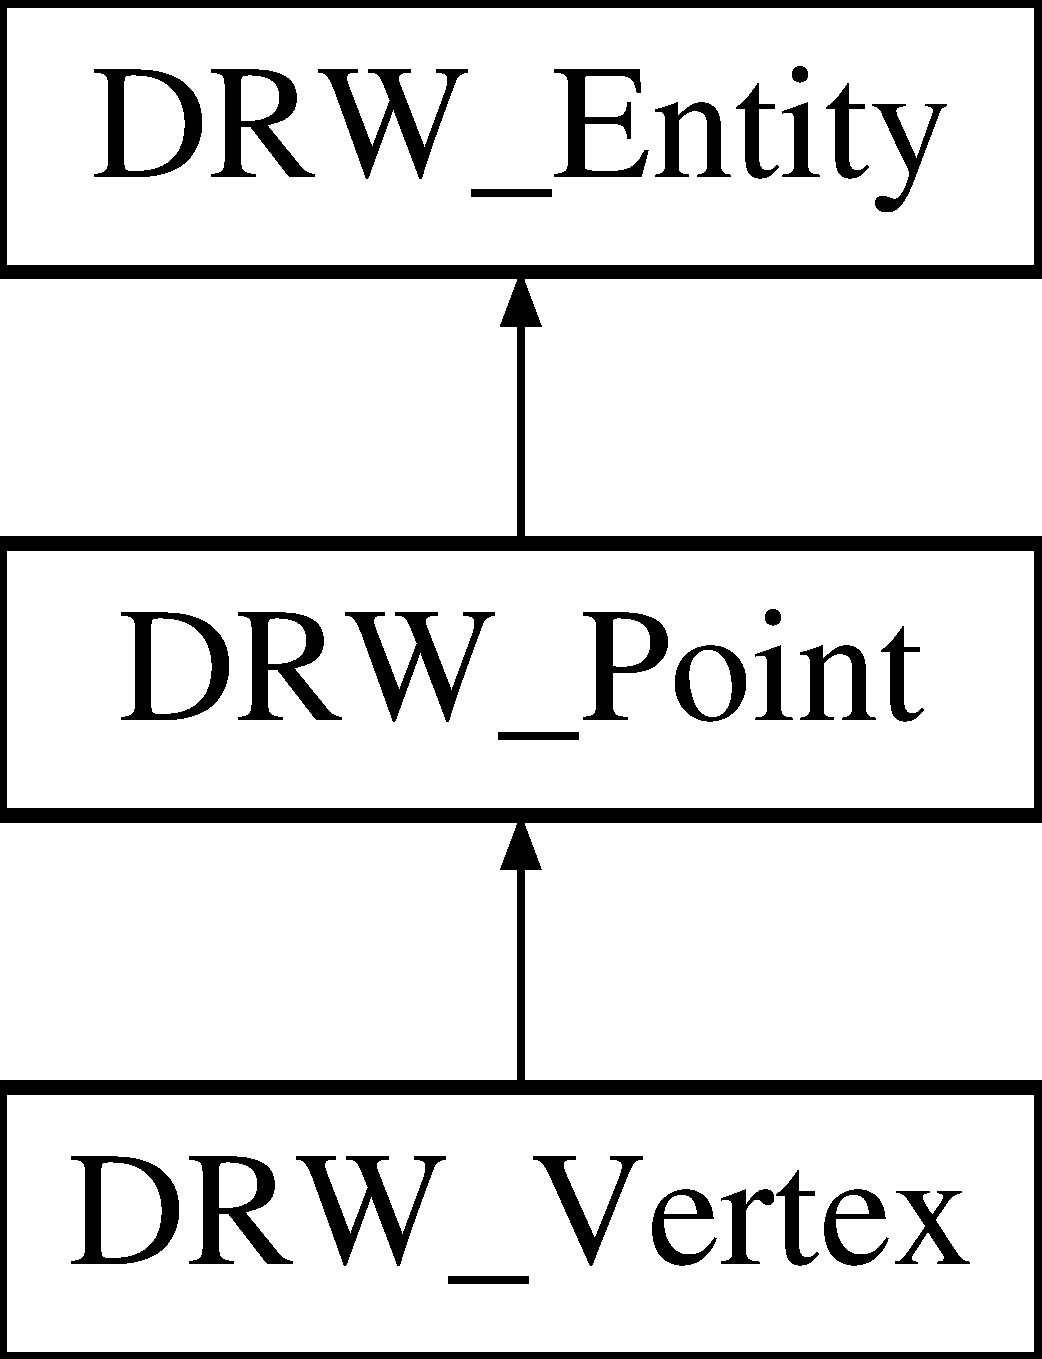
\includegraphics[height=3.000000cm]{df/dc7/class_d_r_w___vertex}
\end{center}
\end{figure}
\subsection*{Public Attributes}
\begin{DoxyCompactItemize}
\item 
double \hyperlink{class_d_r_w___vertex_a59c2c6a18ec24afdec344b187cb89e02}{stawidth}
\item 
double \hyperlink{class_d_r_w___vertex_a707f8fca7c9df740d9a13b1328c05d06}{endwidth}
\item 
double \hyperlink{class_d_r_w___vertex_ace756c96a4ff61eb15e7e1327d7fc56d}{bulge}
\item 
int \hyperlink{class_d_r_w___vertex_a662134a0aaac672cbb37c741e872ce3a}{flags}
\item 
double \hyperlink{class_d_r_w___vertex_ab94318addec1b5ca507a11cf8dd04b34}{tgdir}
\item 
int \hyperlink{class_d_r_w___vertex_aff58612a8e14eb93c6c7667fa19f087b}{vindex1}
\item 
int \hyperlink{class_d_r_w___vertex_a48f459a7d3627c898fa9e1be5b0de6d6}{vindex2}
\item 
int \hyperlink{class_d_r_w___vertex_a43d78abe4c3bacad98ef2a65216e225e}{vindex3}
\item 
int \hyperlink{class_d_r_w___vertex_a1f2c2a799721fe8e6290c6121c190ad8}{vindex4}
\item 
int \hyperlink{class_d_r_w___vertex_a14a4b517273a6c76a5b905eb691d5193}{identifier}
\end{DoxyCompactItemize}
\subsection*{Friends}
\begin{DoxyCompactItemize}
\item 
\hypertarget{class_d_r_w___vertex_a7f080e77e5112f8364c61b97387f8ee2}{}class {\bfseries dxf\+R\+W}\label{class_d_r_w___vertex_a7f080e77e5112f8364c61b97387f8ee2}

\end{DoxyCompactItemize}
\subsection*{Additional Inherited Members}


\subsection{Detailed Description}
Class to handle vertex. 

Class to handle vertex for polyline entity \begin{DoxyAuthor}{Author}
Rallaz 
\end{DoxyAuthor}


\subsection{Member Data Documentation}
\hypertarget{class_d_r_w___vertex_ace756c96a4ff61eb15e7e1327d7fc56d}{}\index{D\+R\+W\+\_\+\+Vertex@{D\+R\+W\+\_\+\+Vertex}!bulge@{bulge}}
\index{bulge@{bulge}!D\+R\+W\+\_\+\+Vertex@{D\+R\+W\+\_\+\+Vertex}}
\subsubsection[{bulge}]{\setlength{\rightskip}{0pt plus 5cm}double D\+R\+W\+\_\+\+Vertex\+::bulge}\label{class_d_r_w___vertex_ace756c96a4ff61eb15e7e1327d7fc56d}
bulge, code 42 \hypertarget{class_d_r_w___vertex_a707f8fca7c9df740d9a13b1328c05d06}{}\index{D\+R\+W\+\_\+\+Vertex@{D\+R\+W\+\_\+\+Vertex}!endwidth@{endwidth}}
\index{endwidth@{endwidth}!D\+R\+W\+\_\+\+Vertex@{D\+R\+W\+\_\+\+Vertex}}
\subsubsection[{endwidth}]{\setlength{\rightskip}{0pt plus 5cm}double D\+R\+W\+\_\+\+Vertex\+::endwidth}\label{class_d_r_w___vertex_a707f8fca7c9df740d9a13b1328c05d06}
End width, code 41 \hypertarget{class_d_r_w___vertex_a662134a0aaac672cbb37c741e872ce3a}{}\index{D\+R\+W\+\_\+\+Vertex@{D\+R\+W\+\_\+\+Vertex}!flags@{flags}}
\index{flags@{flags}!D\+R\+W\+\_\+\+Vertex@{D\+R\+W\+\_\+\+Vertex}}
\subsubsection[{flags}]{\setlength{\rightskip}{0pt plus 5cm}int D\+R\+W\+\_\+\+Vertex\+::flags}\label{class_d_r_w___vertex_a662134a0aaac672cbb37c741e872ce3a}
vertex flag, code 70, default 0 \hypertarget{class_d_r_w___vertex_a14a4b517273a6c76a5b905eb691d5193}{}\index{D\+R\+W\+\_\+\+Vertex@{D\+R\+W\+\_\+\+Vertex}!identifier@{identifier}}
\index{identifier@{identifier}!D\+R\+W\+\_\+\+Vertex@{D\+R\+W\+\_\+\+Vertex}}
\subsubsection[{identifier}]{\setlength{\rightskip}{0pt plus 5cm}int D\+R\+W\+\_\+\+Vertex\+::identifier}\label{class_d_r_w___vertex_a14a4b517273a6c76a5b905eb691d5193}
vertex identifier, code 91, default 0 \hypertarget{class_d_r_w___vertex_a59c2c6a18ec24afdec344b187cb89e02}{}\index{D\+R\+W\+\_\+\+Vertex@{D\+R\+W\+\_\+\+Vertex}!stawidth@{stawidth}}
\index{stawidth@{stawidth}!D\+R\+W\+\_\+\+Vertex@{D\+R\+W\+\_\+\+Vertex}}
\subsubsection[{stawidth}]{\setlength{\rightskip}{0pt plus 5cm}double D\+R\+W\+\_\+\+Vertex\+::stawidth}\label{class_d_r_w___vertex_a59c2c6a18ec24afdec344b187cb89e02}
Start width, code 40 \hypertarget{class_d_r_w___vertex_ab94318addec1b5ca507a11cf8dd04b34}{}\index{D\+R\+W\+\_\+\+Vertex@{D\+R\+W\+\_\+\+Vertex}!tgdir@{tgdir}}
\index{tgdir@{tgdir}!D\+R\+W\+\_\+\+Vertex@{D\+R\+W\+\_\+\+Vertex}}
\subsubsection[{tgdir}]{\setlength{\rightskip}{0pt plus 5cm}double D\+R\+W\+\_\+\+Vertex\+::tgdir}\label{class_d_r_w___vertex_ab94318addec1b5ca507a11cf8dd04b34}
curve fit tangent direction, code 50 \hypertarget{class_d_r_w___vertex_aff58612a8e14eb93c6c7667fa19f087b}{}\index{D\+R\+W\+\_\+\+Vertex@{D\+R\+W\+\_\+\+Vertex}!vindex1@{vindex1}}
\index{vindex1@{vindex1}!D\+R\+W\+\_\+\+Vertex@{D\+R\+W\+\_\+\+Vertex}}
\subsubsection[{vindex1}]{\setlength{\rightskip}{0pt plus 5cm}int D\+R\+W\+\_\+\+Vertex\+::vindex1}\label{class_d_r_w___vertex_aff58612a8e14eb93c6c7667fa19f087b}
polyface mesh vertex index, code 71, default 0 \hypertarget{class_d_r_w___vertex_a48f459a7d3627c898fa9e1be5b0de6d6}{}\index{D\+R\+W\+\_\+\+Vertex@{D\+R\+W\+\_\+\+Vertex}!vindex2@{vindex2}}
\index{vindex2@{vindex2}!D\+R\+W\+\_\+\+Vertex@{D\+R\+W\+\_\+\+Vertex}}
\subsubsection[{vindex2}]{\setlength{\rightskip}{0pt plus 5cm}int D\+R\+W\+\_\+\+Vertex\+::vindex2}\label{class_d_r_w___vertex_a48f459a7d3627c898fa9e1be5b0de6d6}
polyface mesh vertex index, code 72, default 0 \hypertarget{class_d_r_w___vertex_a43d78abe4c3bacad98ef2a65216e225e}{}\index{D\+R\+W\+\_\+\+Vertex@{D\+R\+W\+\_\+\+Vertex}!vindex3@{vindex3}}
\index{vindex3@{vindex3}!D\+R\+W\+\_\+\+Vertex@{D\+R\+W\+\_\+\+Vertex}}
\subsubsection[{vindex3}]{\setlength{\rightskip}{0pt plus 5cm}int D\+R\+W\+\_\+\+Vertex\+::vindex3}\label{class_d_r_w___vertex_a43d78abe4c3bacad98ef2a65216e225e}
polyface mesh vertex index, code 73, default 0 \hypertarget{class_d_r_w___vertex_a1f2c2a799721fe8e6290c6121c190ad8}{}\index{D\+R\+W\+\_\+\+Vertex@{D\+R\+W\+\_\+\+Vertex}!vindex4@{vindex4}}
\index{vindex4@{vindex4}!D\+R\+W\+\_\+\+Vertex@{D\+R\+W\+\_\+\+Vertex}}
\subsubsection[{vindex4}]{\setlength{\rightskip}{0pt plus 5cm}int D\+R\+W\+\_\+\+Vertex\+::vindex4}\label{class_d_r_w___vertex_a1f2c2a799721fe8e6290c6121c190ad8}
polyface mesh vertex index, code 74, default 0 

The documentation for this class was generated from the following files\+:\begin{DoxyCompactItemize}
\item 
src/drw\+\_\+entities.\+h\item 
src/drw\+\_\+entities.\+cpp\end{DoxyCompactItemize}

\hypertarget{class_d_r_w___vertex2_d}{}\section{D\+R\+W\+\_\+\+Vertex2\+D Class Reference}
\label{class_d_r_w___vertex2_d}\index{D\+R\+W\+\_\+\+Vertex2\+D@{D\+R\+W\+\_\+\+Vertex2\+D}}


Class to handle vertex.  




{\ttfamily \#include $<$drw\+\_\+base.\+h$>$}

\subsection*{Public Attributes}
\begin{DoxyCompactItemize}
\item 
double \hyperlink{class_d_r_w___vertex2_d_abe6dee44053f5d82387209e7c76186c8}{x}
\item 
double \hyperlink{class_d_r_w___vertex2_d_a45e73443961543c05bff340dfe14cb8e}{y}
\item 
double \hyperlink{class_d_r_w___vertex2_d_a5d3c878a768fa6c10f158a2bbd9726ca}{stawidth}
\item 
double \hyperlink{class_d_r_w___vertex2_d_a810d285d1f81da75a895ade902e8d159}{endwidth}
\item 
double \hyperlink{class_d_r_w___vertex2_d_a844591ce6d6f01562b831afe4261e99f}{bulge}
\end{DoxyCompactItemize}


\subsection{Detailed Description}
Class to handle vertex. 

Class to handle vertex for lwpolyline entity \begin{DoxyAuthor}{Author}
Rallaz 
\end{DoxyAuthor}


\subsection{Member Data Documentation}
\hypertarget{class_d_r_w___vertex2_d_a844591ce6d6f01562b831afe4261e99f}{}\index{D\+R\+W\+\_\+\+Vertex2\+D@{D\+R\+W\+\_\+\+Vertex2\+D}!bulge@{bulge}}
\index{bulge@{bulge}!D\+R\+W\+\_\+\+Vertex2\+D@{D\+R\+W\+\_\+\+Vertex2\+D}}
\subsubsection[{bulge}]{\setlength{\rightskip}{0pt plus 5cm}double D\+R\+W\+\_\+\+Vertex2\+D\+::bulge}\label{class_d_r_w___vertex2_d_a844591ce6d6f01562b831afe4261e99f}
bulge, code 42 \hypertarget{class_d_r_w___vertex2_d_a810d285d1f81da75a895ade902e8d159}{}\index{D\+R\+W\+\_\+\+Vertex2\+D@{D\+R\+W\+\_\+\+Vertex2\+D}!endwidth@{endwidth}}
\index{endwidth@{endwidth}!D\+R\+W\+\_\+\+Vertex2\+D@{D\+R\+W\+\_\+\+Vertex2\+D}}
\subsubsection[{endwidth}]{\setlength{\rightskip}{0pt plus 5cm}double D\+R\+W\+\_\+\+Vertex2\+D\+::endwidth}\label{class_d_r_w___vertex2_d_a810d285d1f81da75a895ade902e8d159}
End width, code 41 \hypertarget{class_d_r_w___vertex2_d_a5d3c878a768fa6c10f158a2bbd9726ca}{}\index{D\+R\+W\+\_\+\+Vertex2\+D@{D\+R\+W\+\_\+\+Vertex2\+D}!stawidth@{stawidth}}
\index{stawidth@{stawidth}!D\+R\+W\+\_\+\+Vertex2\+D@{D\+R\+W\+\_\+\+Vertex2\+D}}
\subsubsection[{stawidth}]{\setlength{\rightskip}{0pt plus 5cm}double D\+R\+W\+\_\+\+Vertex2\+D\+::stawidth}\label{class_d_r_w___vertex2_d_a5d3c878a768fa6c10f158a2bbd9726ca}
Start width, code 40 \hypertarget{class_d_r_w___vertex2_d_abe6dee44053f5d82387209e7c76186c8}{}\index{D\+R\+W\+\_\+\+Vertex2\+D@{D\+R\+W\+\_\+\+Vertex2\+D}!x@{x}}
\index{x@{x}!D\+R\+W\+\_\+\+Vertex2\+D@{D\+R\+W\+\_\+\+Vertex2\+D}}
\subsubsection[{x}]{\setlength{\rightskip}{0pt plus 5cm}double D\+R\+W\+\_\+\+Vertex2\+D\+::x}\label{class_d_r_w___vertex2_d_abe6dee44053f5d82387209e7c76186c8}
x coordinate, code 10 \hypertarget{class_d_r_w___vertex2_d_a45e73443961543c05bff340dfe14cb8e}{}\index{D\+R\+W\+\_\+\+Vertex2\+D@{D\+R\+W\+\_\+\+Vertex2\+D}!y@{y}}
\index{y@{y}!D\+R\+W\+\_\+\+Vertex2\+D@{D\+R\+W\+\_\+\+Vertex2\+D}}
\subsubsection[{y}]{\setlength{\rightskip}{0pt plus 5cm}double D\+R\+W\+\_\+\+Vertex2\+D\+::y}\label{class_d_r_w___vertex2_d_a45e73443961543c05bff340dfe14cb8e}
y coordinate, code 20 

The documentation for this class was generated from the following file\+:\begin{DoxyCompactItemize}
\item 
src/drw\+\_\+base.\+h\end{DoxyCompactItemize}

\hypertarget{class_d_r_w___viewport}{}\section{D\+R\+W\+\_\+\+Viewport Class Reference}
\label{class_d_r_w___viewport}\index{D\+R\+W\+\_\+\+Viewport@{D\+R\+W\+\_\+\+Viewport}}


Class to handle viewport entity.  




{\ttfamily \#include $<$drw\+\_\+entities.\+h$>$}

Inheritance diagram for D\+R\+W\+\_\+\+Viewport\+:\begin{figure}[H]
\begin{center}
\leavevmode
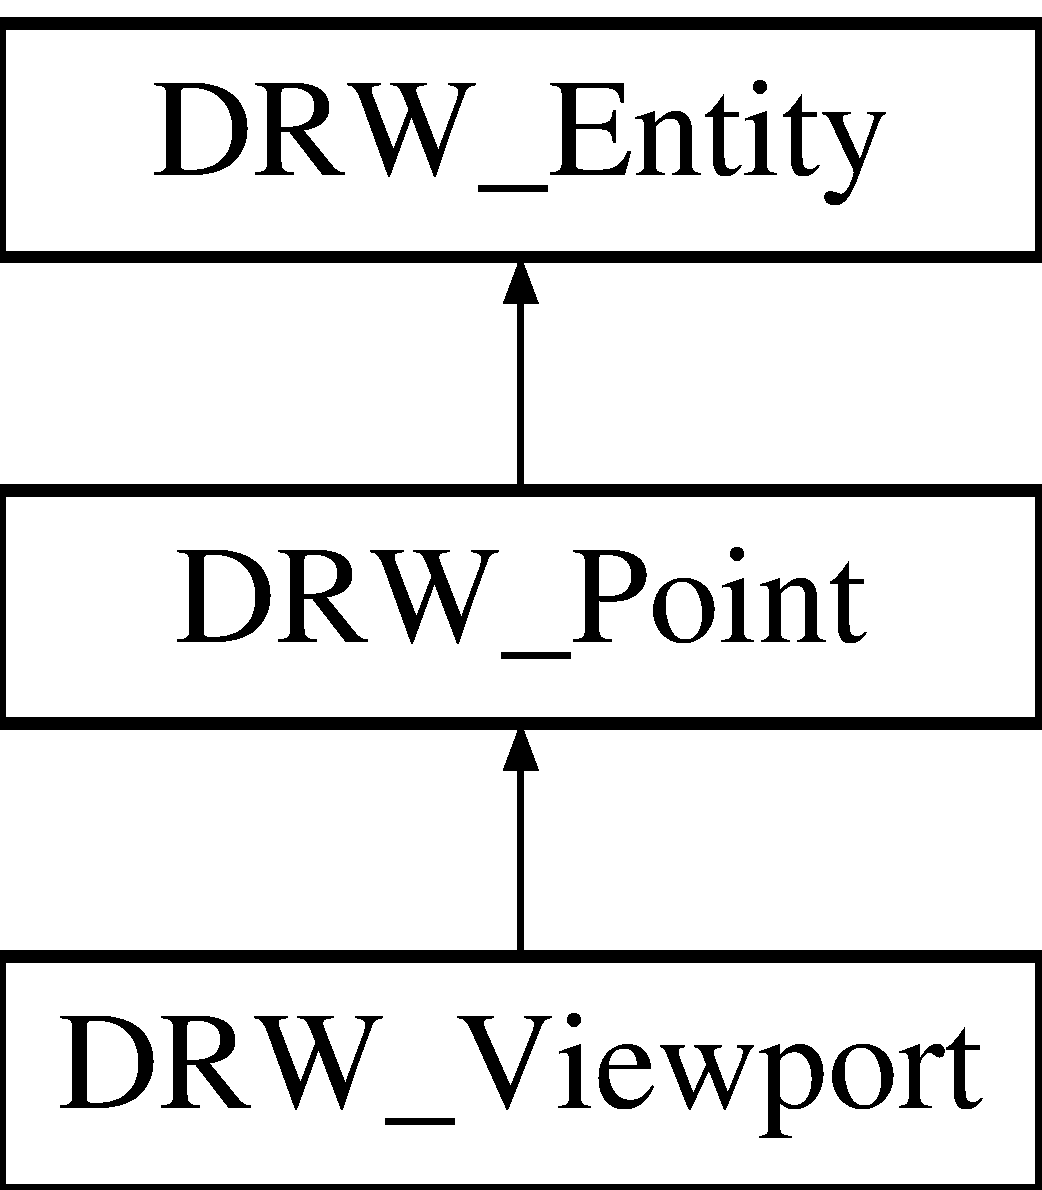
\includegraphics[height=3.000000cm]{da/d35/class_d_r_w___viewport}
\end{center}
\end{figure}
\subsection*{Public Attributes}
\begin{DoxyCompactItemize}
\item 
double \hyperlink{class_d_r_w___viewport_a3d0d03d4fc2c8a3edb3f1ad6e2cdcf2e}{pswidth}
\item 
double \hyperlink{class_d_r_w___viewport_af462ca77d7463df5319af366846b6494}{psheight}
\item 
int \hyperlink{class_d_r_w___viewport_a5d894c4b220ebb89e7b2f368a02c6a65}{vpstatus}
\item 
int \hyperlink{class_d_r_w___viewport_adbec007a8c4b56acd1a55238aca29250}{vp\+I\+D}
\item 
double \hyperlink{class_d_r_w___viewport_a345ae2f37484ce99a63b0a62444a80e9}{center\+P\+X}
\item 
double \hyperlink{class_d_r_w___viewport_aa40e5f6095ea9641c463c71f79bc7650}{center\+P\+Y}
\item 
\hyperlink{class_d_r_w___coord}{D\+R\+W\+\_\+\+Coord} \hyperlink{class_d_r_w___viewport_a7ef3ded922fc5a3c5edd5b8da8a3d3d8}{view\+Dir}
\item 
\hyperlink{class_d_r_w___coord}{D\+R\+W\+\_\+\+Coord} \hyperlink{class_d_r_w___viewport_aa33f15bb04421b33772d4ba7473a272c}{view\+Target}
\item 
double \hyperlink{class_d_r_w___viewport_a5350736f5091de23f63b13586aab6ff5}{view\+Length}
\item 
double \hyperlink{class_d_r_w___viewport_ab09b16c657b284f681b10005b7a691c6}{front\+Clip}
\item 
double \hyperlink{class_d_r_w___viewport_ac43573ecf6007bc2a5223465ab0d3dc0}{back\+Clip}
\item 
double \hyperlink{class_d_r_w___viewport_a58791e7b528bdaaa6f1ca0572c7321ea}{view\+Height}
\item 
double \hyperlink{class_d_r_w___viewport_a6ad208870366d62263d0a6ae190ab4bc}{snap\+Angle}
\item 
double \hyperlink{class_d_r_w___viewport_a0d16a6058735a91ca33cf9b19383ff69}{twist\+Angle}
\end{DoxyCompactItemize}
\subsection*{Additional Inherited Members}


\subsection{Detailed Description}
Class to handle viewport entity. 

Class to handle viewport entity \begin{DoxyAuthor}{Author}
Rallaz 
\end{DoxyAuthor}


\subsection{Member Data Documentation}
\hypertarget{class_d_r_w___viewport_ac43573ecf6007bc2a5223465ab0d3dc0}{}\index{D\+R\+W\+\_\+\+Viewport@{D\+R\+W\+\_\+\+Viewport}!back\+Clip@{back\+Clip}}
\index{back\+Clip@{back\+Clip}!D\+R\+W\+\_\+\+Viewport@{D\+R\+W\+\_\+\+Viewport}}
\subsubsection[{back\+Clip}]{\setlength{\rightskip}{0pt plus 5cm}double D\+R\+W\+\_\+\+Viewport\+::back\+Clip}\label{class_d_r_w___viewport_ac43573ecf6007bc2a5223465ab0d3dc0}
Back clip plane Z value, code 44 \hypertarget{class_d_r_w___viewport_a345ae2f37484ce99a63b0a62444a80e9}{}\index{D\+R\+W\+\_\+\+Viewport@{D\+R\+W\+\_\+\+Viewport}!center\+P\+X@{center\+P\+X}}
\index{center\+P\+X@{center\+P\+X}!D\+R\+W\+\_\+\+Viewport@{D\+R\+W\+\_\+\+Viewport}}
\subsubsection[{center\+P\+X}]{\setlength{\rightskip}{0pt plus 5cm}double D\+R\+W\+\_\+\+Viewport\+::center\+P\+X}\label{class_d_r_w___viewport_a345ae2f37484ce99a63b0a62444a80e9}
view center point X, code 12 \hypertarget{class_d_r_w___viewport_aa40e5f6095ea9641c463c71f79bc7650}{}\index{D\+R\+W\+\_\+\+Viewport@{D\+R\+W\+\_\+\+Viewport}!center\+P\+Y@{center\+P\+Y}}
\index{center\+P\+Y@{center\+P\+Y}!D\+R\+W\+\_\+\+Viewport@{D\+R\+W\+\_\+\+Viewport}}
\subsubsection[{center\+P\+Y}]{\setlength{\rightskip}{0pt plus 5cm}double D\+R\+W\+\_\+\+Viewport\+::center\+P\+Y}\label{class_d_r_w___viewport_aa40e5f6095ea9641c463c71f79bc7650}
view center point Y, code 22 \hypertarget{class_d_r_w___viewport_ab09b16c657b284f681b10005b7a691c6}{}\index{D\+R\+W\+\_\+\+Viewport@{D\+R\+W\+\_\+\+Viewport}!front\+Clip@{front\+Clip}}
\index{front\+Clip@{front\+Clip}!D\+R\+W\+\_\+\+Viewport@{D\+R\+W\+\_\+\+Viewport}}
\subsubsection[{front\+Clip}]{\setlength{\rightskip}{0pt plus 5cm}double D\+R\+W\+\_\+\+Viewport\+::front\+Clip}\label{class_d_r_w___viewport_ab09b16c657b284f681b10005b7a691c6}
Front clip plane Z value, code 43 \hypertarget{class_d_r_w___viewport_af462ca77d7463df5319af366846b6494}{}\index{D\+R\+W\+\_\+\+Viewport@{D\+R\+W\+\_\+\+Viewport}!psheight@{psheight}}
\index{psheight@{psheight}!D\+R\+W\+\_\+\+Viewport@{D\+R\+W\+\_\+\+Viewport}}
\subsubsection[{psheight}]{\setlength{\rightskip}{0pt plus 5cm}double D\+R\+W\+\_\+\+Viewport\+::psheight}\label{class_d_r_w___viewport_af462ca77d7463df5319af366846b6494}
Height in paper space units, code 41 \hypertarget{class_d_r_w___viewport_a3d0d03d4fc2c8a3edb3f1ad6e2cdcf2e}{}\index{D\+R\+W\+\_\+\+Viewport@{D\+R\+W\+\_\+\+Viewport}!pswidth@{pswidth}}
\index{pswidth@{pswidth}!D\+R\+W\+\_\+\+Viewport@{D\+R\+W\+\_\+\+Viewport}}
\subsubsection[{pswidth}]{\setlength{\rightskip}{0pt plus 5cm}double D\+R\+W\+\_\+\+Viewport\+::pswidth}\label{class_d_r_w___viewport_a3d0d03d4fc2c8a3edb3f1ad6e2cdcf2e}
Width in paper space units, code 40 \hypertarget{class_d_r_w___viewport_a6ad208870366d62263d0a6ae190ab4bc}{}\index{D\+R\+W\+\_\+\+Viewport@{D\+R\+W\+\_\+\+Viewport}!snap\+Angle@{snap\+Angle}}
\index{snap\+Angle@{snap\+Angle}!D\+R\+W\+\_\+\+Viewport@{D\+R\+W\+\_\+\+Viewport}}
\subsubsection[{snap\+Angle}]{\setlength{\rightskip}{0pt plus 5cm}double D\+R\+W\+\_\+\+Viewport\+::snap\+Angle}\label{class_d_r_w___viewport_a6ad208870366d62263d0a6ae190ab4bc}
Snap angle, code 50 \hypertarget{class_d_r_w___viewport_a0d16a6058735a91ca33cf9b19383ff69}{}\index{D\+R\+W\+\_\+\+Viewport@{D\+R\+W\+\_\+\+Viewport}!twist\+Angle@{twist\+Angle}}
\index{twist\+Angle@{twist\+Angle}!D\+R\+W\+\_\+\+Viewport@{D\+R\+W\+\_\+\+Viewport}}
\subsubsection[{twist\+Angle}]{\setlength{\rightskip}{0pt plus 5cm}double D\+R\+W\+\_\+\+Viewport\+::twist\+Angle}\label{class_d_r_w___viewport_a0d16a6058735a91ca33cf9b19383ff69}
view twist angle, code 51 \hypertarget{class_d_r_w___viewport_a7ef3ded922fc5a3c5edd5b8da8a3d3d8}{}\index{D\+R\+W\+\_\+\+Viewport@{D\+R\+W\+\_\+\+Viewport}!view\+Dir@{view\+Dir}}
\index{view\+Dir@{view\+Dir}!D\+R\+W\+\_\+\+Viewport@{D\+R\+W\+\_\+\+Viewport}}
\subsubsection[{view\+Dir}]{\setlength{\rightskip}{0pt plus 5cm}{\bf D\+R\+W\+\_\+\+Coord} D\+R\+W\+\_\+\+Viewport\+::view\+Dir}\label{class_d_r_w___viewport_a7ef3ded922fc5a3c5edd5b8da8a3d3d8}
View direction vector, code 16 \hypertarget{class_d_r_w___viewport_a58791e7b528bdaaa6f1ca0572c7321ea}{}\index{D\+R\+W\+\_\+\+Viewport@{D\+R\+W\+\_\+\+Viewport}!view\+Height@{view\+Height}}
\index{view\+Height@{view\+Height}!D\+R\+W\+\_\+\+Viewport@{D\+R\+W\+\_\+\+Viewport}}
\subsubsection[{view\+Height}]{\setlength{\rightskip}{0pt plus 5cm}double D\+R\+W\+\_\+\+Viewport\+::view\+Height}\label{class_d_r_w___viewport_a58791e7b528bdaaa6f1ca0572c7321ea}
View height in model space units, code 45 \hypertarget{class_d_r_w___viewport_a5350736f5091de23f63b13586aab6ff5}{}\index{D\+R\+W\+\_\+\+Viewport@{D\+R\+W\+\_\+\+Viewport}!view\+Length@{view\+Length}}
\index{view\+Length@{view\+Length}!D\+R\+W\+\_\+\+Viewport@{D\+R\+W\+\_\+\+Viewport}}
\subsubsection[{view\+Length}]{\setlength{\rightskip}{0pt plus 5cm}double D\+R\+W\+\_\+\+Viewport\+::view\+Length}\label{class_d_r_w___viewport_a5350736f5091de23f63b13586aab6ff5}
Perspective lens length, code 42 \hypertarget{class_d_r_w___viewport_aa33f15bb04421b33772d4ba7473a272c}{}\index{D\+R\+W\+\_\+\+Viewport@{D\+R\+W\+\_\+\+Viewport}!view\+Target@{view\+Target}}
\index{view\+Target@{view\+Target}!D\+R\+W\+\_\+\+Viewport@{D\+R\+W\+\_\+\+Viewport}}
\subsubsection[{view\+Target}]{\setlength{\rightskip}{0pt plus 5cm}{\bf D\+R\+W\+\_\+\+Coord} D\+R\+W\+\_\+\+Viewport\+::view\+Target}\label{class_d_r_w___viewport_aa33f15bb04421b33772d4ba7473a272c}
View target point, code 17 \hypertarget{class_d_r_w___viewport_adbec007a8c4b56acd1a55238aca29250}{}\index{D\+R\+W\+\_\+\+Viewport@{D\+R\+W\+\_\+\+Viewport}!vp\+I\+D@{vp\+I\+D}}
\index{vp\+I\+D@{vp\+I\+D}!D\+R\+W\+\_\+\+Viewport@{D\+R\+W\+\_\+\+Viewport}}
\subsubsection[{vp\+I\+D}]{\setlength{\rightskip}{0pt plus 5cm}int D\+R\+W\+\_\+\+Viewport\+::vp\+I\+D}\label{class_d_r_w___viewport_adbec007a8c4b56acd1a55238aca29250}
Viewport I\+D, code 69 \hypertarget{class_d_r_w___viewport_a5d894c4b220ebb89e7b2f368a02c6a65}{}\index{D\+R\+W\+\_\+\+Viewport@{D\+R\+W\+\_\+\+Viewport}!vpstatus@{vpstatus}}
\index{vpstatus@{vpstatus}!D\+R\+W\+\_\+\+Viewport@{D\+R\+W\+\_\+\+Viewport}}
\subsubsection[{vpstatus}]{\setlength{\rightskip}{0pt plus 5cm}int D\+R\+W\+\_\+\+Viewport\+::vpstatus}\label{class_d_r_w___viewport_a5d894c4b220ebb89e7b2f368a02c6a65}
Viewport status, code 68 

The documentation for this class was generated from the following files\+:\begin{DoxyCompactItemize}
\item 
src/drw\+\_\+entities.\+h\item 
src/drw\+\_\+entities.\+cpp\end{DoxyCompactItemize}

\hypertarget{class_d_r_w___vport}{}\section{D\+R\+W\+\_\+\+Vport Class Reference}
\label{class_d_r_w___vport}\index{D\+R\+W\+\_\+\+Vport@{D\+R\+W\+\_\+\+Vport}}


Class to handle vport entries.  




{\ttfamily \#include $<$drw\+\_\+objects.\+h$>$}

Inheritance diagram for D\+R\+W\+\_\+\+Vport\+:\begin{figure}[H]
\begin{center}
\leavevmode
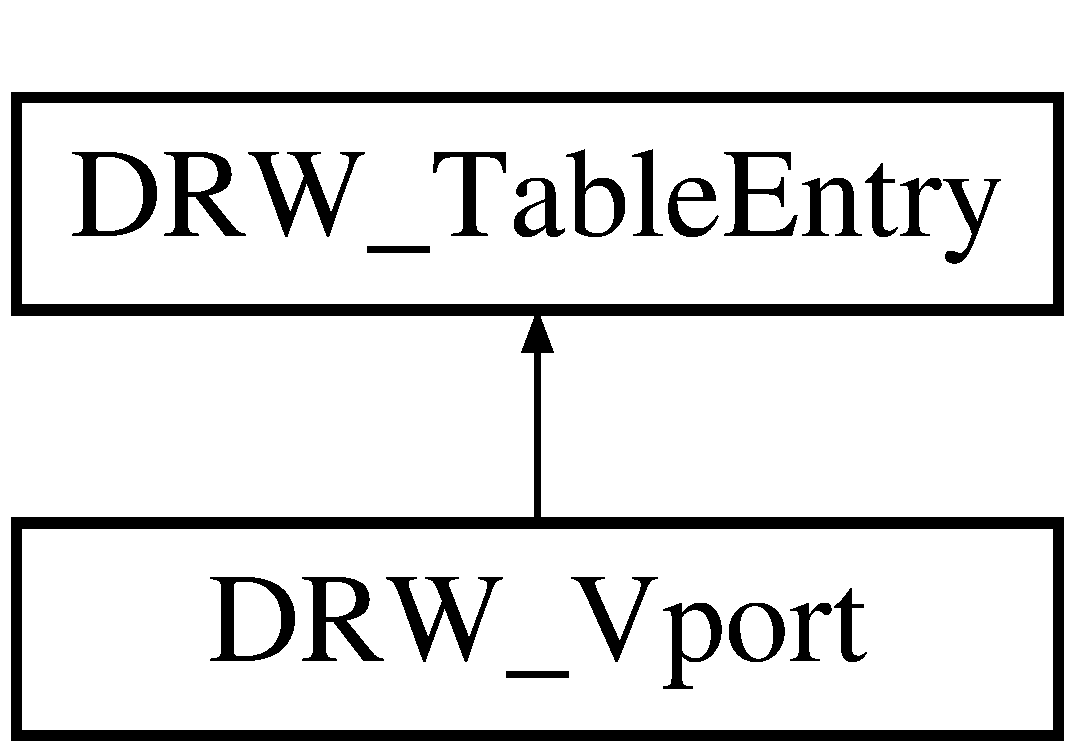
\includegraphics[height=2.000000cm]{db/daa/class_d_r_w___vport}
\end{center}
\end{figure}
\subsection*{Public Member Functions}
\begin{DoxyCompactItemize}
\item 
void \hyperlink{class_d_r_w___vport_a7f865bb07bda60869ece9c15b7ceb186}{parse\+Code} (int code, dxf\+Reader $\ast$reader)
\begin{DoxyCompactList}\small\item\em Class to handle vport entries. \end{DoxyCompactList}\end{DoxyCompactItemize}
\subsection*{Public Attributes}
\begin{DoxyCompactItemize}
\item 
\hyperlink{class_d_r_w___coord}{D\+R\+W\+\_\+\+Coord} \hyperlink{class_d_r_w___vport_a27df49d3aacabe83be11ac29463f75c1}{lower\+Left}
\item 
\hyperlink{class_d_r_w___coord}{D\+R\+W\+\_\+\+Coord} \hyperlink{class_d_r_w___vport_ae63541133c20a69a6e13f25191e02b05}{Upper\+Right}
\item 
\hyperlink{class_d_r_w___coord}{D\+R\+W\+\_\+\+Coord} \hyperlink{class_d_r_w___vport_a56104afc60b9fb0b8c6682982f92a45e}{center}
\item 
\hyperlink{class_d_r_w___coord}{D\+R\+W\+\_\+\+Coord} \hyperlink{class_d_r_w___vport_a152be2cc28b499c29e9302efa54e001c}{snap\+Base}
\item 
\hyperlink{class_d_r_w___coord}{D\+R\+W\+\_\+\+Coord} \hyperlink{class_d_r_w___vport_a19aa53d1282cb737b21fa3d3b60d3b20}{snap\+Spacing}
\item 
\hyperlink{class_d_r_w___coord}{D\+R\+W\+\_\+\+Coord} \hyperlink{class_d_r_w___vport_a0284747ef8bda7287e99534d9fdc75e5}{grid\+Spacing}
\item 
\hyperlink{class_d_r_w___coord}{D\+R\+W\+\_\+\+Coord} \hyperlink{class_d_r_w___vport_a657f3b92d041527a5a485dce22c448a1}{view\+Dir}
\item 
\hyperlink{class_d_r_w___coord}{D\+R\+W\+\_\+\+Coord} \hyperlink{class_d_r_w___vport_a93eb77539e5ad11990b828074685d85f}{view\+Target}
\item 
double \hyperlink{class_d_r_w___vport_aae2ac1375b707a159d317051a9ff4e9e}{height}
\item 
double \hyperlink{class_d_r_w___vport_ab84331826a4e1bd181eb2ca6a55e4a97}{ratio}
\item 
double \hyperlink{class_d_r_w___vport_a9d3e2b640f9f9791d50b00f5cae452f9}{lens\+Height}
\item 
double \hyperlink{class_d_r_w___vport_a2ee10a71212915501bfdbaa532ec7107}{front\+Clip}
\item 
double \hyperlink{class_d_r_w___vport_a160e2ab229be33a622e4f888eb4295c7}{back\+Clip}
\item 
double \hyperlink{class_d_r_w___vport_a1709ba5680cf5b0bf9c7b41bab479225}{snap\+Angle}
\item 
double \hyperlink{class_d_r_w___vport_a2705ee0b61e21b33cad269b71c04b86c}{twist\+Angle}
\item 
int \hyperlink{class_d_r_w___vport_ab96feaf67d7eed371e30ffdf04a4a9cb}{view\+Mode}
\item 
int \hyperlink{class_d_r_w___vport_afdff3db96e16473300e9c2d50b464267}{circle\+Zoom}
\item 
int \hyperlink{class_d_r_w___vport_a2e8e4ad00361daa81e7cdcd3ffc51d4f}{fast\+Zoom}
\item 
int \hyperlink{class_d_r_w___vport_ac3bd19802da31bd4bb9e07255e0bbdc6}{ucs\+Icon}
\item 
int \hyperlink{class_d_r_w___vport_a9a358c56a549eba62bb326fdcc510bb2}{snap}
\item 
int \hyperlink{class_d_r_w___vport_afd06c82134688b83439ab917d399eaa6}{grid}
\item 
int \hyperlink{class_d_r_w___vport_a09eede75fea3bb3052edfc9caf5fd380}{snap\+Style}
\item 
int \hyperlink{class_d_r_w___vport_ab69959b8dfaf2ce024b4babee4466445}{snap\+Isopair}
\item 
int \hyperlink{class_d_r_w___vport_a44d1f134682b67fc14a92e468677f493}{grid\+Behavior}
\end{DoxyCompactItemize}
\subsection*{Additional Inherited Members}


\subsection{Detailed Description}
Class to handle vport entries. 

Class to handle vport symbol table entries \begin{DoxyAuthor}{Author}
Rallaz 
\end{DoxyAuthor}


\subsection{Member Function Documentation}
\hypertarget{class_d_r_w___vport_a7f865bb07bda60869ece9c15b7ceb186}{}\index{D\+R\+W\+\_\+\+Vport@{D\+R\+W\+\_\+\+Vport}!parse\+Code@{parse\+Code}}
\index{parse\+Code@{parse\+Code}!D\+R\+W\+\_\+\+Vport@{D\+R\+W\+\_\+\+Vport}}
\subsubsection[{parse\+Code}]{\setlength{\rightskip}{0pt plus 5cm}void D\+R\+W\+\_\+\+Vport\+::parse\+Code (
\begin{DoxyParamCaption}
\item[{int}]{code, }
\item[{dxf\+Reader $\ast$}]{reader}
\end{DoxyParamCaption}
)}\label{class_d_r_w___vport_a7f865bb07bda60869ece9c15b7ceb186}


Class to handle vport entries. 

Class to handle vport symbol table entries \begin{DoxyAuthor}{Author}
Rallaz 
\end{DoxyAuthor}


\subsection{Member Data Documentation}
\hypertarget{class_d_r_w___vport_a160e2ab229be33a622e4f888eb4295c7}{}\index{D\+R\+W\+\_\+\+Vport@{D\+R\+W\+\_\+\+Vport}!back\+Clip@{back\+Clip}}
\index{back\+Clip@{back\+Clip}!D\+R\+W\+\_\+\+Vport@{D\+R\+W\+\_\+\+Vport}}
\subsubsection[{back\+Clip}]{\setlength{\rightskip}{0pt plus 5cm}double D\+R\+W\+\_\+\+Vport\+::back\+Clip}\label{class_d_r_w___vport_a160e2ab229be33a622e4f888eb4295c7}
back clipping plane, code 44 \hypertarget{class_d_r_w___vport_a56104afc60b9fb0b8c6682982f92a45e}{}\index{D\+R\+W\+\_\+\+Vport@{D\+R\+W\+\_\+\+Vport}!center@{center}}
\index{center@{center}!D\+R\+W\+\_\+\+Vport@{D\+R\+W\+\_\+\+Vport}}
\subsubsection[{center}]{\setlength{\rightskip}{0pt plus 5cm}{\bf D\+R\+W\+\_\+\+Coord} D\+R\+W\+\_\+\+Vport\+::center}\label{class_d_r_w___vport_a56104afc60b9fb0b8c6682982f92a45e}
center point in W\+C\+S, code 12 \& 22 \hypertarget{class_d_r_w___vport_afdff3db96e16473300e9c2d50b464267}{}\index{D\+R\+W\+\_\+\+Vport@{D\+R\+W\+\_\+\+Vport}!circle\+Zoom@{circle\+Zoom}}
\index{circle\+Zoom@{circle\+Zoom}!D\+R\+W\+\_\+\+Vport@{D\+R\+W\+\_\+\+Vport}}
\subsubsection[{circle\+Zoom}]{\setlength{\rightskip}{0pt plus 5cm}int D\+R\+W\+\_\+\+Vport\+::circle\+Zoom}\label{class_d_r_w___vport_afdff3db96e16473300e9c2d50b464267}
circle zoom percent, code 72 \hypertarget{class_d_r_w___vport_a2e8e4ad00361daa81e7cdcd3ffc51d4f}{}\index{D\+R\+W\+\_\+\+Vport@{D\+R\+W\+\_\+\+Vport}!fast\+Zoom@{fast\+Zoom}}
\index{fast\+Zoom@{fast\+Zoom}!D\+R\+W\+\_\+\+Vport@{D\+R\+W\+\_\+\+Vport}}
\subsubsection[{fast\+Zoom}]{\setlength{\rightskip}{0pt plus 5cm}int D\+R\+W\+\_\+\+Vport\+::fast\+Zoom}\label{class_d_r_w___vport_a2e8e4ad00361daa81e7cdcd3ffc51d4f}
fast zoom setting, code 73 \hypertarget{class_d_r_w___vport_a2ee10a71212915501bfdbaa532ec7107}{}\index{D\+R\+W\+\_\+\+Vport@{D\+R\+W\+\_\+\+Vport}!front\+Clip@{front\+Clip}}
\index{front\+Clip@{front\+Clip}!D\+R\+W\+\_\+\+Vport@{D\+R\+W\+\_\+\+Vport}}
\subsubsection[{front\+Clip}]{\setlength{\rightskip}{0pt plus 5cm}double D\+R\+W\+\_\+\+Vport\+::front\+Clip}\label{class_d_r_w___vport_a2ee10a71212915501bfdbaa532ec7107}
front clipping plane, code 43 \hypertarget{class_d_r_w___vport_afd06c82134688b83439ab917d399eaa6}{}\index{D\+R\+W\+\_\+\+Vport@{D\+R\+W\+\_\+\+Vport}!grid@{grid}}
\index{grid@{grid}!D\+R\+W\+\_\+\+Vport@{D\+R\+W\+\_\+\+Vport}}
\subsubsection[{grid}]{\setlength{\rightskip}{0pt plus 5cm}int D\+R\+W\+\_\+\+Vport\+::grid}\label{class_d_r_w___vport_afd06c82134688b83439ab917d399eaa6}
grid on/off, code 76 \hypertarget{class_d_r_w___vport_a44d1f134682b67fc14a92e468677f493}{}\index{D\+R\+W\+\_\+\+Vport@{D\+R\+W\+\_\+\+Vport}!grid\+Behavior@{grid\+Behavior}}
\index{grid\+Behavior@{grid\+Behavior}!D\+R\+W\+\_\+\+Vport@{D\+R\+W\+\_\+\+Vport}}
\subsubsection[{grid\+Behavior}]{\setlength{\rightskip}{0pt plus 5cm}int D\+R\+W\+\_\+\+Vport\+::grid\+Behavior}\label{class_d_r_w___vport_a44d1f134682b67fc14a92e468677f493}
grid behavior, code 60, undocummented \hypertarget{class_d_r_w___vport_a0284747ef8bda7287e99534d9fdc75e5}{}\index{D\+R\+W\+\_\+\+Vport@{D\+R\+W\+\_\+\+Vport}!grid\+Spacing@{grid\+Spacing}}
\index{grid\+Spacing@{grid\+Spacing}!D\+R\+W\+\_\+\+Vport@{D\+R\+W\+\_\+\+Vport}}
\subsubsection[{grid\+Spacing}]{\setlength{\rightskip}{0pt plus 5cm}{\bf D\+R\+W\+\_\+\+Coord} D\+R\+W\+\_\+\+Vport\+::grid\+Spacing}\label{class_d_r_w___vport_a0284747ef8bda7287e99534d9fdc75e5}
grid Spacing, code 15 \& 25 \hypertarget{class_d_r_w___vport_aae2ac1375b707a159d317051a9ff4e9e}{}\index{D\+R\+W\+\_\+\+Vport@{D\+R\+W\+\_\+\+Vport}!height@{height}}
\index{height@{height}!D\+R\+W\+\_\+\+Vport@{D\+R\+W\+\_\+\+Vport}}
\subsubsection[{height}]{\setlength{\rightskip}{0pt plus 5cm}double D\+R\+W\+\_\+\+Vport\+::height}\label{class_d_r_w___vport_aae2ac1375b707a159d317051a9ff4e9e}
view height, code 40 \hypertarget{class_d_r_w___vport_a9d3e2b640f9f9791d50b00f5cae452f9}{}\index{D\+R\+W\+\_\+\+Vport@{D\+R\+W\+\_\+\+Vport}!lens\+Height@{lens\+Height}}
\index{lens\+Height@{lens\+Height}!D\+R\+W\+\_\+\+Vport@{D\+R\+W\+\_\+\+Vport}}
\subsubsection[{lens\+Height}]{\setlength{\rightskip}{0pt plus 5cm}double D\+R\+W\+\_\+\+Vport\+::lens\+Height}\label{class_d_r_w___vport_a9d3e2b640f9f9791d50b00f5cae452f9}
lens height, code 42 \hypertarget{class_d_r_w___vport_a27df49d3aacabe83be11ac29463f75c1}{}\index{D\+R\+W\+\_\+\+Vport@{D\+R\+W\+\_\+\+Vport}!lower\+Left@{lower\+Left}}
\index{lower\+Left@{lower\+Left}!D\+R\+W\+\_\+\+Vport@{D\+R\+W\+\_\+\+Vport}}
\subsubsection[{lower\+Left}]{\setlength{\rightskip}{0pt plus 5cm}{\bf D\+R\+W\+\_\+\+Coord} D\+R\+W\+\_\+\+Vport\+::lower\+Left}\label{class_d_r_w___vport_a27df49d3aacabe83be11ac29463f75c1}
Lower left corner, code 10 \& 20 \hypertarget{class_d_r_w___vport_ab84331826a4e1bd181eb2ca6a55e4a97}{}\index{D\+R\+W\+\_\+\+Vport@{D\+R\+W\+\_\+\+Vport}!ratio@{ratio}}
\index{ratio@{ratio}!D\+R\+W\+\_\+\+Vport@{D\+R\+W\+\_\+\+Vport}}
\subsubsection[{ratio}]{\setlength{\rightskip}{0pt plus 5cm}double D\+R\+W\+\_\+\+Vport\+::ratio}\label{class_d_r_w___vport_ab84331826a4e1bd181eb2ca6a55e4a97}
viewport aspect ratio, code 41 \hypertarget{class_d_r_w___vport_a9a358c56a549eba62bb326fdcc510bb2}{}\index{D\+R\+W\+\_\+\+Vport@{D\+R\+W\+\_\+\+Vport}!snap@{snap}}
\index{snap@{snap}!D\+R\+W\+\_\+\+Vport@{D\+R\+W\+\_\+\+Vport}}
\subsubsection[{snap}]{\setlength{\rightskip}{0pt plus 5cm}int D\+R\+W\+\_\+\+Vport\+::snap}\label{class_d_r_w___vport_a9a358c56a549eba62bb326fdcc510bb2}
snap on/off, code 75 \hypertarget{class_d_r_w___vport_a1709ba5680cf5b0bf9c7b41bab479225}{}\index{D\+R\+W\+\_\+\+Vport@{D\+R\+W\+\_\+\+Vport}!snap\+Angle@{snap\+Angle}}
\index{snap\+Angle@{snap\+Angle}!D\+R\+W\+\_\+\+Vport@{D\+R\+W\+\_\+\+Vport}}
\subsubsection[{snap\+Angle}]{\setlength{\rightskip}{0pt plus 5cm}double D\+R\+W\+\_\+\+Vport\+::snap\+Angle}\label{class_d_r_w___vport_a1709ba5680cf5b0bf9c7b41bab479225}
snap rotation angle, code 50 \hypertarget{class_d_r_w___vport_a152be2cc28b499c29e9302efa54e001c}{}\index{D\+R\+W\+\_\+\+Vport@{D\+R\+W\+\_\+\+Vport}!snap\+Base@{snap\+Base}}
\index{snap\+Base@{snap\+Base}!D\+R\+W\+\_\+\+Vport@{D\+R\+W\+\_\+\+Vport}}
\subsubsection[{snap\+Base}]{\setlength{\rightskip}{0pt plus 5cm}{\bf D\+R\+W\+\_\+\+Coord} D\+R\+W\+\_\+\+Vport\+::snap\+Base}\label{class_d_r_w___vport_a152be2cc28b499c29e9302efa54e001c}
snap base point in D\+C\+S, code 13 \& 23 \hypertarget{class_d_r_w___vport_ab69959b8dfaf2ce024b4babee4466445}{}\index{D\+R\+W\+\_\+\+Vport@{D\+R\+W\+\_\+\+Vport}!snap\+Isopair@{snap\+Isopair}}
\index{snap\+Isopair@{snap\+Isopair}!D\+R\+W\+\_\+\+Vport@{D\+R\+W\+\_\+\+Vport}}
\subsubsection[{snap\+Isopair}]{\setlength{\rightskip}{0pt plus 5cm}int D\+R\+W\+\_\+\+Vport\+::snap\+Isopair}\label{class_d_r_w___vport_ab69959b8dfaf2ce024b4babee4466445}
snap isopair, code 78 \hypertarget{class_d_r_w___vport_a19aa53d1282cb737b21fa3d3b60d3b20}{}\index{D\+R\+W\+\_\+\+Vport@{D\+R\+W\+\_\+\+Vport}!snap\+Spacing@{snap\+Spacing}}
\index{snap\+Spacing@{snap\+Spacing}!D\+R\+W\+\_\+\+Vport@{D\+R\+W\+\_\+\+Vport}}
\subsubsection[{snap\+Spacing}]{\setlength{\rightskip}{0pt plus 5cm}{\bf D\+R\+W\+\_\+\+Coord} D\+R\+W\+\_\+\+Vport\+::snap\+Spacing}\label{class_d_r_w___vport_a19aa53d1282cb737b21fa3d3b60d3b20}
snap Spacing, code 14 \& 24 \hypertarget{class_d_r_w___vport_a09eede75fea3bb3052edfc9caf5fd380}{}\index{D\+R\+W\+\_\+\+Vport@{D\+R\+W\+\_\+\+Vport}!snap\+Style@{snap\+Style}}
\index{snap\+Style@{snap\+Style}!D\+R\+W\+\_\+\+Vport@{D\+R\+W\+\_\+\+Vport}}
\subsubsection[{snap\+Style}]{\setlength{\rightskip}{0pt plus 5cm}int D\+R\+W\+\_\+\+Vport\+::snap\+Style}\label{class_d_r_w___vport_a09eede75fea3bb3052edfc9caf5fd380}
snap style, code 77 \hypertarget{class_d_r_w___vport_a2705ee0b61e21b33cad269b71c04b86c}{}\index{D\+R\+W\+\_\+\+Vport@{D\+R\+W\+\_\+\+Vport}!twist\+Angle@{twist\+Angle}}
\index{twist\+Angle@{twist\+Angle}!D\+R\+W\+\_\+\+Vport@{D\+R\+W\+\_\+\+Vport}}
\subsubsection[{twist\+Angle}]{\setlength{\rightskip}{0pt plus 5cm}double D\+R\+W\+\_\+\+Vport\+::twist\+Angle}\label{class_d_r_w___vport_a2705ee0b61e21b33cad269b71c04b86c}
view twist angle, code 51 \hypertarget{class_d_r_w___vport_ac3bd19802da31bd4bb9e07255e0bbdc6}{}\index{D\+R\+W\+\_\+\+Vport@{D\+R\+W\+\_\+\+Vport}!ucs\+Icon@{ucs\+Icon}}
\index{ucs\+Icon@{ucs\+Icon}!D\+R\+W\+\_\+\+Vport@{D\+R\+W\+\_\+\+Vport}}
\subsubsection[{ucs\+Icon}]{\setlength{\rightskip}{0pt plus 5cm}int D\+R\+W\+\_\+\+Vport\+::ucs\+Icon}\label{class_d_r_w___vport_ac3bd19802da31bd4bb9e07255e0bbdc6}
U\+C\+S\+I\+C\+O\+N setting, code 74 \hypertarget{class_d_r_w___vport_ae63541133c20a69a6e13f25191e02b05}{}\index{D\+R\+W\+\_\+\+Vport@{D\+R\+W\+\_\+\+Vport}!Upper\+Right@{Upper\+Right}}
\index{Upper\+Right@{Upper\+Right}!D\+R\+W\+\_\+\+Vport@{D\+R\+W\+\_\+\+Vport}}
\subsubsection[{Upper\+Right}]{\setlength{\rightskip}{0pt plus 5cm}{\bf D\+R\+W\+\_\+\+Coord} D\+R\+W\+\_\+\+Vport\+::\+Upper\+Right}\label{class_d_r_w___vport_ae63541133c20a69a6e13f25191e02b05}
Upper right corner, code 11 \& 21 \hypertarget{class_d_r_w___vport_a657f3b92d041527a5a485dce22c448a1}{}\index{D\+R\+W\+\_\+\+Vport@{D\+R\+W\+\_\+\+Vport}!view\+Dir@{view\+Dir}}
\index{view\+Dir@{view\+Dir}!D\+R\+W\+\_\+\+Vport@{D\+R\+W\+\_\+\+Vport}}
\subsubsection[{view\+Dir}]{\setlength{\rightskip}{0pt plus 5cm}{\bf D\+R\+W\+\_\+\+Coord} D\+R\+W\+\_\+\+Vport\+::view\+Dir}\label{class_d_r_w___vport_a657f3b92d041527a5a485dce22c448a1}
view direction from target point, code 16, 26 \& 36 \hypertarget{class_d_r_w___vport_ab96feaf67d7eed371e30ffdf04a4a9cb}{}\index{D\+R\+W\+\_\+\+Vport@{D\+R\+W\+\_\+\+Vport}!view\+Mode@{view\+Mode}}
\index{view\+Mode@{view\+Mode}!D\+R\+W\+\_\+\+Vport@{D\+R\+W\+\_\+\+Vport}}
\subsubsection[{view\+Mode}]{\setlength{\rightskip}{0pt plus 5cm}int D\+R\+W\+\_\+\+Vport\+::view\+Mode}\label{class_d_r_w___vport_ab96feaf67d7eed371e30ffdf04a4a9cb}
view mode, code 71 \hypertarget{class_d_r_w___vport_a93eb77539e5ad11990b828074685d85f}{}\index{D\+R\+W\+\_\+\+Vport@{D\+R\+W\+\_\+\+Vport}!view\+Target@{view\+Target}}
\index{view\+Target@{view\+Target}!D\+R\+W\+\_\+\+Vport@{D\+R\+W\+\_\+\+Vport}}
\subsubsection[{view\+Target}]{\setlength{\rightskip}{0pt plus 5cm}{\bf D\+R\+W\+\_\+\+Coord} D\+R\+W\+\_\+\+Vport\+::view\+Target}\label{class_d_r_w___vport_a93eb77539e5ad11990b828074685d85f}
view target point, code 17, 27 \& 37 

The documentation for this class was generated from the following files\+:\begin{DoxyCompactItemize}
\item 
src/drw\+\_\+objects.\+h\item 
src/drw\+\_\+objects.\+cpp\end{DoxyCompactItemize}

\hypertarget{class_d_r_w___xline}{}\section{D\+R\+W\+\_\+\+Xline Class Reference}
\label{class_d_r_w___xline}\index{D\+R\+W\+\_\+\+Xline@{D\+R\+W\+\_\+\+Xline}}


Class to handle xline entity.  




{\ttfamily \#include $<$drw\+\_\+entities.\+h$>$}

Inheritance diagram for D\+R\+W\+\_\+\+Xline\+:\begin{figure}[H]
\begin{center}
\leavevmode
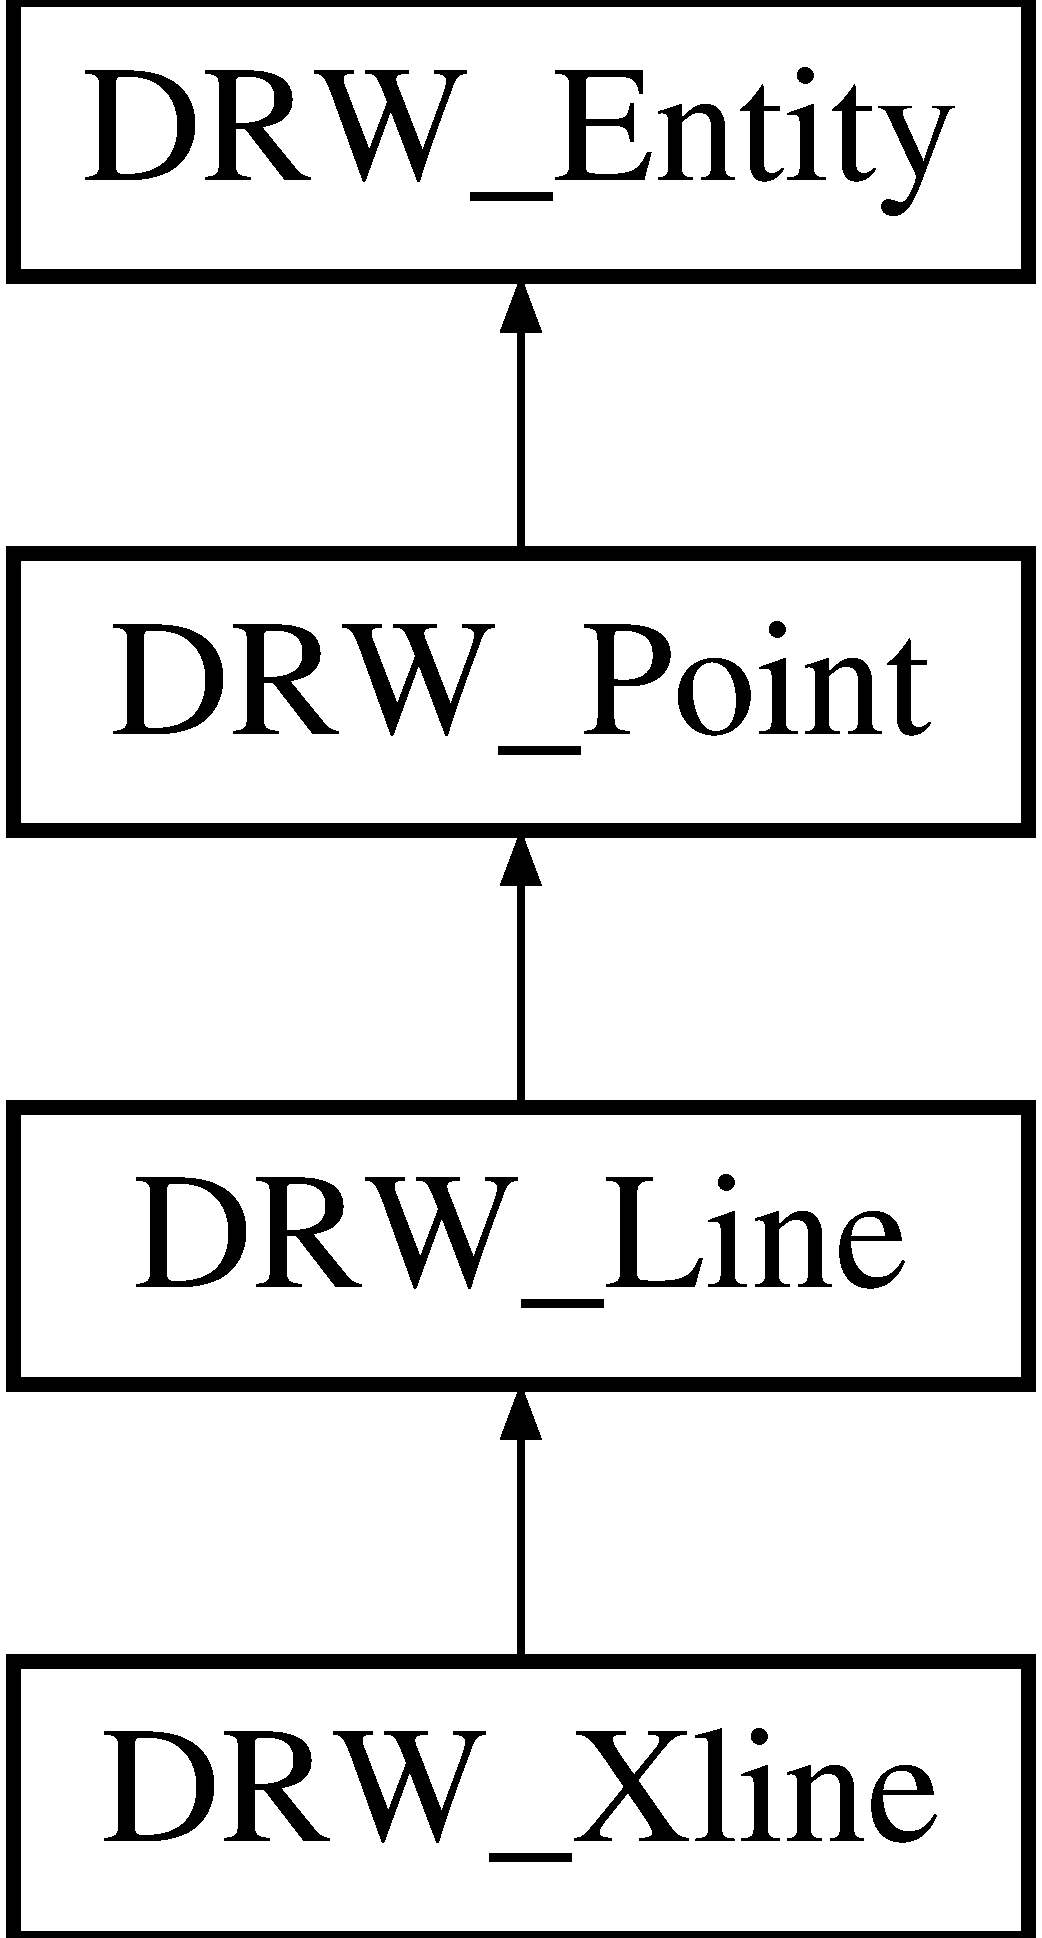
\includegraphics[height=4.000000cm]{d7/d68/class_d_r_w___xline}
\end{center}
\end{figure}
\subsection*{Additional Inherited Members}


\subsection{Detailed Description}
Class to handle xline entity. 

Class to handle xline entity \begin{DoxyAuthor}{Author}
Rallaz 
\end{DoxyAuthor}


The documentation for this class was generated from the following file\+:\begin{DoxyCompactItemize}
\item 
src/drw\+\_\+entities.\+h\end{DoxyCompactItemize}

\hypertarget{classdwg_handle}{}\section{dwg\+Handle Class Reference}
\label{classdwg_handle}\index{dwg\+Handle@{dwg\+Handle}}


Class to handle dwg handles.  




{\ttfamily \#include $<$drw\+\_\+base.\+h$>$}



\subsection{Detailed Description}
Class to handle dwg handles. 

Class to handle dwg handles \begin{DoxyAuthor}{Author}
Rallaz 
\end{DoxyAuthor}


The documentation for this class was generated from the following file\+:\begin{DoxyCompactItemize}
\item 
src/drw\+\_\+base.\+h\end{DoxyCompactItemize}

\hypertarget{classdwg_r}{}\section{dwg\+R Class Reference}
\label{classdwg_r}\index{dwg\+R@{dwg\+R}}


The documentation for this class was generated from the following files\+:\begin{DoxyCompactItemize}
\item 
src/libdwgr.\+h\item 
src/libdwgr.\+cpp\end{DoxyCompactItemize}

\hypertarget{classdxf_r_w}{}\section{dxf\+R\+W Class Reference}
\label{classdxf_r_w}\index{dxf\+R\+W@{dxf\+R\+W}}
\subsection*{Public Member Functions}
\begin{DoxyCompactItemize}
\item 
bool \hyperlink{classdxf_r_w_ab3262753c90b34d8911691cdddaf7bfa}{read} (\hyperlink{class_d_r_w___interface}{D\+R\+W\+\_\+\+Interface} $\ast$interface\+\_\+, bool ext)
\begin{DoxyCompactList}\small\item\em reads the file specified in constructor \end{DoxyCompactList}\item 
void \hyperlink{classdxf_r_w_a6eb61de3ea383636bedc049d23d7e759}{set\+Ellipse\+Parts} (int parts)
\end{DoxyCompactItemize}
\subsection*{Private Member Functions}
\begin{DoxyCompactItemize}
\item 
\hypertarget{classdxf_r_w_ab0d6afb7e2d297a292fcf2fe8af742b8}{}bool \hyperlink{classdxf_r_w_ab0d6afb7e2d297a292fcf2fe8af742b8}{process\+Dxf} ()\label{classdxf_r_w_ab0d6afb7e2d297a292fcf2fe8af742b8}

\begin{DoxyCompactList}\small\item\em used by \hyperlink{classdxf_r_w_ab3262753c90b34d8911691cdddaf7bfa}{read()} to parse the content of the file \end{DoxyCompactList}\item 
std\+::string \hyperlink{classdxf_r_w_ac8c55be7454779ae2039aca405049860}{to\+Hex\+Str} (int n)
\end{DoxyCompactItemize}
\subsection*{Private Attributes}
\begin{DoxyCompactItemize}
\item 
int \hyperlink{classdxf_r_w_aee251f0e7de9a814aa04b3cc9f2fa7a8}{el\+Parts}
\item 
std\+::vector$<$ \hyperlink{class_d_r_w___image_def}{D\+R\+W\+\_\+\+Image\+Def} $\ast$ $>$ \hyperlink{classdxf_r_w_ad90dd62fa6c58393eeb6baea1c777175}{image\+Def}
\end{DoxyCompactItemize}


\subsection{Member Function Documentation}
\hypertarget{classdxf_r_w_ab3262753c90b34d8911691cdddaf7bfa}{}\index{dxf\+R\+W@{dxf\+R\+W}!read@{read}}
\index{read@{read}!dxf\+R\+W@{dxf\+R\+W}}
\subsubsection[{read}]{\setlength{\rightskip}{0pt plus 5cm}bool dxf\+R\+W\+::read (
\begin{DoxyParamCaption}
\item[{{\bf D\+R\+W\+\_\+\+Interface} $\ast$}]{interface\+\_\+, }
\item[{bool}]{ext}
\end{DoxyParamCaption}
)}\label{classdxf_r_w_ab3262753c90b34d8911691cdddaf7bfa}


reads the file specified in constructor 

An interface must be provided. It is used by the class to signal various components being added. 
\begin{DoxyParams}{Parameters}
{\em interface\+\_\+} & the interface to use \\
\hline
{\em ext} & should the extrusion be applied to convert in 2\+D? \\
\hline
\end{DoxyParams}
\begin{DoxyReturn}{Returns}
true for success 
\end{DoxyReturn}
\hypertarget{classdxf_r_w_a6eb61de3ea383636bedc049d23d7e759}{}\index{dxf\+R\+W@{dxf\+R\+W}!set\+Ellipse\+Parts@{set\+Ellipse\+Parts}}
\index{set\+Ellipse\+Parts@{set\+Ellipse\+Parts}!dxf\+R\+W@{dxf\+R\+W}}
\subsubsection[{set\+Ellipse\+Parts}]{\setlength{\rightskip}{0pt plus 5cm}void dxf\+R\+W\+::set\+Ellipse\+Parts (
\begin{DoxyParamCaption}
\item[{int}]{parts}
\end{DoxyParamCaption}
)\hspace{0.3cm}{\ttfamily [inline]}}\label{classdxf_r_w_a6eb61de3ea383636bedc049d23d7e759}
set parts munber when convert ellipse to polyline \hypertarget{classdxf_r_w_ac8c55be7454779ae2039aca405049860}{}\index{dxf\+R\+W@{dxf\+R\+W}!to\+Hex\+Str@{to\+Hex\+Str}}
\index{to\+Hex\+Str@{to\+Hex\+Str}!dxf\+R\+W@{dxf\+R\+W}}
\subsubsection[{to\+Hex\+Str}]{\setlength{\rightskip}{0pt plus 5cm}std\+::string dxf\+R\+W\+::to\+Hex\+Str (
\begin{DoxyParamCaption}
\item[{int}]{n}
\end{DoxyParamCaption}
)\hspace{0.3cm}{\ttfamily [private]}}\label{classdxf_r_w_ac8c55be7454779ae2039aca405049860}
utility function convert a int to string in hex 

\subsection{Member Data Documentation}
\hypertarget{classdxf_r_w_aee251f0e7de9a814aa04b3cc9f2fa7a8}{}\index{dxf\+R\+W@{dxf\+R\+W}!el\+Parts@{el\+Parts}}
\index{el\+Parts@{el\+Parts}!dxf\+R\+W@{dxf\+R\+W}}
\subsubsection[{el\+Parts}]{\setlength{\rightskip}{0pt plus 5cm}int dxf\+R\+W\+::el\+Parts\hspace{0.3cm}{\ttfamily [private]}}\label{classdxf_r_w_aee251f0e7de9a814aa04b3cc9f2fa7a8}
parts munber when convert ellipse to polyline \hypertarget{classdxf_r_w_ad90dd62fa6c58393eeb6baea1c777175}{}\index{dxf\+R\+W@{dxf\+R\+W}!image\+Def@{image\+Def}}
\index{image\+Def@{image\+Def}!dxf\+R\+W@{dxf\+R\+W}}
\subsubsection[{image\+Def}]{\setlength{\rightskip}{0pt plus 5cm}std\+::vector$<${\bf D\+R\+W\+\_\+\+Image\+Def}$\ast$$>$ dxf\+R\+W\+::image\+Def\hspace{0.3cm}{\ttfamily [private]}}\label{classdxf_r_w_ad90dd62fa6c58393eeb6baea1c777175}
image\+Def list 

The documentation for this class was generated from the following files\+:\begin{DoxyCompactItemize}
\item 
src/libdxfrw.\+h\item 
src/libdxfrw.\+cpp\end{DoxyCompactItemize}

\hypertarget{struct_d_r_w_1_1_group}{}\section{D\+R\+W\+:\+:Group Struct Reference}
\label{struct_d_r_w_1_1_group}\index{D\+R\+W\+::\+Group@{D\+R\+W\+::\+Group}}


A group in dxf file.  




{\ttfamily \#include $<$drw\+\_\+base.\+h$>$}



\subsection{Detailed Description}
A group in dxf file. 

The documentation for this struct was generated from the following file\+:\begin{DoxyCompactItemize}
\item 
src/drw\+\_\+base.\+h\end{DoxyCompactItemize}

%--- End generated contents ---

% Index
\backmatter
\newpage
\phantomsection
\clearemptydoublepage
\addcontentsline{toc}{chapter}{Index}
\printindex

\end{document}
